% Options for packages loaded elsewhere
% Options for packages loaded elsewhere
\PassOptionsToPackage{unicode}{hyperref}
\PassOptionsToPackage{hyphens}{url}
\PassOptionsToPackage{dvipsnames,svgnames,x11names}{xcolor}
%
\documentclass[
  10pt,
  a4paper,
  DIV=11,
  numbers=noendperiod,
  oneside]{scrreprt}
\usepackage{xcolor}
\usepackage[top=12mm,bottom=13mm,left=14mm,right=14mm,headheight=14pt,headsep=6mm,footskip=8mm,headsep=4mm,footskip=6mm,includeheadfoot,heightrounded]{geometry}
\usepackage{amsmath,amssymb}
\setcounter{secnumdepth}{4}
\usepackage{iftex}
\ifPDFTeX
  \usepackage[T1]{fontenc}
  \usepackage[utf8]{inputenc}
  \usepackage{textcomp} % provide euro and other symbols
\else % if luatex or xetex
  \usepackage{unicode-math} % this also loads fontspec
  \defaultfontfeatures{Scale=MatchLowercase}
  \defaultfontfeatures[\rmfamily]{Ligatures=TeX,Scale=1}
\fi
\usepackage{lmodern}
\ifPDFTeX\else
  % xetex/luatex font selection
\fi
% Use upquote if available, for straight quotes in verbatim environments
\IfFileExists{upquote.sty}{\usepackage{upquote}}{}
\IfFileExists{microtype.sty}{% use microtype if available
  \usepackage[]{microtype}
  \UseMicrotypeSet[protrusion]{basicmath} % disable protrusion for tt fonts
}{}
\makeatletter
\@ifundefined{KOMAClassName}{% if non-KOMA class
  \IfFileExists{parskip.sty}{%
    \usepackage{parskip}
  }{% else
    \setlength{\parindent}{0pt}
    \setlength{\parskip}{6pt plus 2pt minus 1pt}}
}{% if KOMA class
  \KOMAoptions{parskip=half}}
\makeatother
% Make \paragraph and \subparagraph free-standing
\makeatletter
\ifx\paragraph\undefined\else
  \let\oldparagraph\paragraph
  \renewcommand{\paragraph}{
    \@ifstar
      \xxxParagraphStar
      \xxxParagraphNoStar
  }
  \newcommand{\xxxParagraphStar}[1]{\oldparagraph*{#1}\mbox{}}
  \newcommand{\xxxParagraphNoStar}[1]{\oldparagraph{#1}\mbox{}}
\fi
\ifx\subparagraph\undefined\else
  \let\oldsubparagraph\subparagraph
  \renewcommand{\subparagraph}{
    \@ifstar
      \xxxSubParagraphStar
      \xxxSubParagraphNoStar
  }
  \newcommand{\xxxSubParagraphStar}[1]{\oldsubparagraph*{#1}\mbox{}}
  \newcommand{\xxxSubParagraphNoStar}[1]{\oldsubparagraph{#1}\mbox{}}
\fi
\makeatother

\usepackage{color}
\usepackage{fancyvrb}
\newcommand{\VerbBar}{|}
\newcommand{\VERB}{\Verb[commandchars=\\\{\}]}
\DefineVerbatimEnvironment{Highlighting}{Verbatim}{commandchars=\\\{\}}
% Add ',fontsize=\small' for more characters per line
\usepackage{framed}
\definecolor{shadecolor}{RGB}{241,243,245}
\newenvironment{Shaded}{\begin{snugshade}}{\end{snugshade}}
\newcommand{\AlertTok}[1]{\textcolor[rgb]{0.68,0.00,0.00}{#1}}
\newcommand{\AnnotationTok}[1]{\textcolor[rgb]{0.37,0.37,0.37}{#1}}
\newcommand{\AttributeTok}[1]{\textcolor[rgb]{0.40,0.45,0.13}{#1}}
\newcommand{\BaseNTok}[1]{\textcolor[rgb]{0.68,0.00,0.00}{#1}}
\newcommand{\BuiltInTok}[1]{\textcolor[rgb]{0.00,0.23,0.31}{#1}}
\newcommand{\CharTok}[1]{\textcolor[rgb]{0.13,0.47,0.30}{#1}}
\newcommand{\CommentTok}[1]{\textcolor[rgb]{0.37,0.37,0.37}{#1}}
\newcommand{\CommentVarTok}[1]{\textcolor[rgb]{0.37,0.37,0.37}{\textit{#1}}}
\newcommand{\ConstantTok}[1]{\textcolor[rgb]{0.56,0.35,0.01}{#1}}
\newcommand{\ControlFlowTok}[1]{\textcolor[rgb]{0.00,0.23,0.31}{\textbf{#1}}}
\newcommand{\DataTypeTok}[1]{\textcolor[rgb]{0.68,0.00,0.00}{#1}}
\newcommand{\DecValTok}[1]{\textcolor[rgb]{0.68,0.00,0.00}{#1}}
\newcommand{\DocumentationTok}[1]{\textcolor[rgb]{0.37,0.37,0.37}{\textit{#1}}}
\newcommand{\ErrorTok}[1]{\textcolor[rgb]{0.68,0.00,0.00}{#1}}
\newcommand{\ExtensionTok}[1]{\textcolor[rgb]{0.00,0.23,0.31}{#1}}
\newcommand{\FloatTok}[1]{\textcolor[rgb]{0.68,0.00,0.00}{#1}}
\newcommand{\FunctionTok}[1]{\textcolor[rgb]{0.28,0.35,0.67}{#1}}
\newcommand{\ImportTok}[1]{\textcolor[rgb]{0.00,0.46,0.62}{#1}}
\newcommand{\InformationTok}[1]{\textcolor[rgb]{0.37,0.37,0.37}{#1}}
\newcommand{\KeywordTok}[1]{\textcolor[rgb]{0.00,0.23,0.31}{\textbf{#1}}}
\newcommand{\NormalTok}[1]{\textcolor[rgb]{0.00,0.23,0.31}{#1}}
\newcommand{\OperatorTok}[1]{\textcolor[rgb]{0.37,0.37,0.37}{#1}}
\newcommand{\OtherTok}[1]{\textcolor[rgb]{0.00,0.23,0.31}{#1}}
\newcommand{\PreprocessorTok}[1]{\textcolor[rgb]{0.68,0.00,0.00}{#1}}
\newcommand{\RegionMarkerTok}[1]{\textcolor[rgb]{0.00,0.23,0.31}{#1}}
\newcommand{\SpecialCharTok}[1]{\textcolor[rgb]{0.37,0.37,0.37}{#1}}
\newcommand{\SpecialStringTok}[1]{\textcolor[rgb]{0.13,0.47,0.30}{#1}}
\newcommand{\StringTok}[1]{\textcolor[rgb]{0.13,0.47,0.30}{#1}}
\newcommand{\VariableTok}[1]{\textcolor[rgb]{0.07,0.07,0.07}{#1}}
\newcommand{\VerbatimStringTok}[1]{\textcolor[rgb]{0.13,0.47,0.30}{#1}}
\newcommand{\WarningTok}[1]{\textcolor[rgb]{0.37,0.37,0.37}{\textit{#1}}}

\usepackage{longtable,booktabs,array}
\newcounter{none} % for unnumbered tables
\usepackage{calc} % for calculating minipage widths
% Correct order of tables after \paragraph or \subparagraph
\usepackage{etoolbox}
\makeatletter
\patchcmd\longtable{\par}{\if@noskipsec\mbox{}\fi\par}{}{}
\makeatother
% Allow footnotes in longtable head/foot
\IfFileExists{footnotehyper.sty}{\usepackage{footnotehyper}}{\usepackage{footnote}}
\makesavenoteenv{longtable}
\usepackage{graphicx}
\makeatletter
\newsavebox\pandoc@box
\newcommand*\pandocbounded[1]{% scales image to fit in text height/width
  \sbox\pandoc@box{#1}%
  \Gscale@div\@tempa{\textheight}{\dimexpr\ht\pandoc@box+\dp\pandoc@box\relax}%
  \Gscale@div\@tempb{\linewidth}{\wd\pandoc@box}%
  \ifdim\@tempb\p@<\@tempa\p@\let\@tempa\@tempb\fi% select the smaller of both
  \ifdim\@tempa\p@<\p@\scalebox{\@tempa}{\usebox\pandoc@box}%
  \else\usebox{\pandoc@box}%
  \fi%
}
% Set default figure placement to htbp
\def\fps@figure{htbp}
\makeatother


% definitions for citeproc citations
\NewDocumentCommand\citeproctext{}{}
\NewDocumentCommand\citeproc{mm}{%
  \begingroup\def\citeproctext{#2}\cite{#1}\endgroup}
\makeatletter
 % allow citations to break across lines
 \let\@cite@ofmt\@firstofone
 % avoid brackets around text for \cite:
 \def\@biblabel#1{}
 \def\@cite#1#2{{#1\if@tempswa , #2\fi}}
\makeatother
\newlength{\cslhangindent}
\setlength{\cslhangindent}{1.5em}
\newlength{\csllabelwidth}
\setlength{\csllabelwidth}{3em}
\newenvironment{CSLReferences}[2] % #1 hanging-indent, #2 entry-spacing
 {\begin{list}{}{%
  \setlength{\itemindent}{0pt}
  \setlength{\leftmargin}{0pt}
  \setlength{\parsep}{0pt}
  % turn on hanging indent if param 1 is 1
  \ifodd #1
   \setlength{\leftmargin}{\cslhangindent}
   \setlength{\itemindent}{-1\cslhangindent}
  \fi
  % set entry spacing
  \setlength{\itemsep}{#2\baselineskip}}}
 {\end{list}}
\usepackage{calc}
\newcommand{\CSLBlock}[1]{\hfill\break\parbox[t]{\linewidth}{\strut\ignorespaces#1\strut}}
\newcommand{\CSLLeftMargin}[1]{\parbox[t]{\csllabelwidth}{\strut#1\strut}}
\newcommand{\CSLRightInline}[1]{\parbox[t]{\linewidth - \csllabelwidth}{\strut#1\strut}}
\newcommand{\CSLIndent}[1]{\hspace{\cslhangindent}#1}



\setlength{\emergencystretch}{3em} % prevent overfull lines

\providecommand{\tightlist}{%
  \setlength{\itemsep}{0pt}\setlength{\parskip}{0pt}}



 


% CleanMyMap - configuration Quarto PDF officielle.
% Ce fichier règle uniquement la mise en page. Il ne modifie pas le contenu du rapport.

\usepackage{fontspec}
\usepackage{booktabs}
\usepackage{longtable}
\usepackage{array}
\usepackage{tabularx}
\usepackage{makecell}
\usepackage{pdflscape}
\usepackage{float}
\usepackage{graphicx}
\usepackage{xcolor}
\usepackage{colortbl}
\usepackage{xurl}
\usepackage{fancyhdr}
\usepackage{titlesec}
\usepackage{titling}
\usepackage{microtype}
\usepackage{indentfirst}
\usepackage{fvextra}
\usepackage{etoolbox}
\usepackage{needspace}
\usepackage{caption}
\usepackage{enumitem}
\usepackage{setspace}
\usepackage{tikz}
\usepackage{eso-pic}
\usepackage[most]{tcolorbox}

% Polices institutionnelles
\IfFontExistsTF{Inter}{
  \setmainfont{Inter}
  \setsansfont{Inter}
}{
  \setmainfont{Arial}
  \setsansfont{Arial}
}
\renewcommand*\familydefault{\sfdefault}

% Couleurs institutionnelles
\definecolor{cmmnavy}{HTML}{1A365D}
\definecolor{cmmblue}{HTML}{2563A8}
\definecolor{cmmteal}{HTML}{1F6F78}
\definecolor{cmmgreen}{HTML}{2F7D5E}
\definecolor{cmmwarm}{HTML}{8A5A24}
\definecolor{cmmgray}{HTML}{5A6772}
\definecolor{cmmrule}{HTML}{B8C8D0}
\definecolor{cmmlight}{HTML}{EAF2F4}
\definecolor{cmmgreenlight}{HTML}{EDF7F0}
\definecolor{cmmnotelight}{HTML}{F2F7F8}
\definecolor{cmmwarmlight}{HTML}{FFF7E8}
\definecolor{cmmtablehead}{HTML}{E1EEF2}
\definecolor{quarto-callout-note-color}{HTML}{2563A8}
\definecolor{quarto-callout-tip-color}{HTML}{2F7D5E}
\definecolor{quarto-callout-important-color}{HTML}{8A5A24}
\definecolor{quarto-callout-warning-color}{HTML}{8A5A24}
\definecolor{quarto-callout-caution-color}{HTML}{8A5A24}

% Liens cliquables et lisibles
\AtBeginDocument{
  \hypersetup{
    colorlinks=true,
    linkcolor=cmmblue,
    urlcolor=cmmblue,
    citecolor=cmmblue,
    bookmarksopen=true,
    bookmarksnumbered=true,
    pdfborder={0 0 0}
  }
}
\urlstyle{same}

% Lisibilité générale
\setstretch{1.1}
\setlength{\parindent}{1.15em}
\setlength{\parskip}{4.8pt plus 1pt minus 1pt}
\raggedbottom
\emergencystretch=4em
\sloppy

% Listes compactes mais respirantes
\setlist[itemize]{topsep=4pt,itemsep=2.5pt,parsep=0pt,leftmargin=1.35em}
\setlist[enumerate]{topsep=4pt,itemsep=2.5pt,parsep=0pt,leftmargin=1.6em}

% Pied de page minimal : numéro de page uniquement
\pagestyle{fancy}
\fancyhf{}
\fancyfoot[C]{\footnotesize\textcolor{cmmgray}{\thepage}}
\renewcommand{\headrulewidth}{0pt}
\renewcommand{\footrulewidth}{0pt}

\fancypagestyle{plain}{
  \fancyhf{}
  \fancyfoot[C]{\footnotesize\textcolor{cmmgray}{\thepage}}
  \renewcommand{\headrulewidth}{0pt}
  \renewcommand{\footrulewidth}{0pt}
}

% Grandes parties : nouvelle page sans créer de page de chapitre.
\newcommand{\sectionbreak}{\clearpage}

% Titres hiérarchisés et protégés contre les titres orphelins.
\titleformat{\section}
  {\Needspace{8\baselineskip}\color{cmmnavy}\normalfont\fontsize{20pt}{24pt}\selectfont\bfseries}
  {\thesection}{0.8em}{}
  [\vspace{0.18em}\color{cmmrule}\titlerule]

\titleformat{\subsection}
  {\Needspace{5\baselineskip}\color{cmmteal}\normalfont\fontsize{14pt}{17pt}\selectfont\bfseries}
  {\thesubsection}{0.7em}{}

\titleformat{\subsubsection}
  {\Needspace{4\baselineskip}\color{cmmnavy}\normalfont\fontsize{11.5pt}{14pt}\selectfont\bfseries}
  {\thesubsubsection}{0.6em}{}

\titleformat{\paragraph}[runin]
  {\color{cmmblue}\normalfont\normalsize\bfseries}
  {}{0em}{}[. ]

\titlespacing*{\section}{0pt}{0.9em}{0.8em}
\titlespacing*{\subsection}{0pt}{0.85em}{0.4em}
\titlespacing*{\subsubsection}{0pt}{0.6em}{0.28em}

% Emphases sobres : le soulignement reste réservé aux liens.
\let\oldtextbf\textbf
\renewcommand{\textbf}[1]{\oldtextbf{\textcolor{cmmnavy}{#1}}}
\let\oldemph\emph
\renewcommand{\emph}[1]{\oldemph{\textcolor{cmmgray}{#1}}}

% Tableaux lisibles sur A4 étroit
\setlength{\tabcolsep}{4.5pt}
\renewcommand{\arraystretch}{1.2}
\setlength{\LTleft}{0pt}
\setlength{\LTright}{0pt}
\setlength{\LTcapwidth}{\textwidth}
\captionsetup{font=small, labelfont=bf}
\arrayrulecolor{cmmrule}
\AtBeginEnvironment{longtable}{\small\arrayrulecolor{cmmrule}}
\AtBeginEnvironment{tabular}{\small\arrayrulecolor{cmmrule}}
\AtBeginEnvironment{table}{\small}
\newcolumntype{L}[1]{>{\raggedright\arraybackslash}p{#1}}

% Code, liens longs et citations
\fvset{breaklines=true,breakanywhere=true,fontsize=\small}
\AtBeginEnvironment{quote}{\small\color{cmmgray}}

% Encadrés Quarto : rendu sobre et académique.
\tcbset{
  enhanced,
  boxrule=0pt,
  leftrule=2.2pt,
  arc=1.2mm,
  outer arc=1.2mm,
  boxsep=2.5pt,
  left=6pt,
  right=6pt,
  top=5pt,
  bottom=5pt,
  before skip=8pt,
  after skip=8pt,
  fonttitle=\bfseries\color{cmmnavy},
  coltitle=cmmnavy,
  colback=cmmnotelight,
  colframe=cmmblue,
  coltext=black
}

\AtBeginEnvironment{tcolorbox}{\small}
\AtBeginEnvironment{table}{\Needspace{6\baselineskip}}

% Page de garde personnalisée
\pretitle{
  \AddToShipoutPictureBG*{
    \AtPageCenter{
      \makebox[0pt]{
        \begin{tikzpicture}[remember picture,overlay]
          \node[opacity=0.08] at (current page.center) {
            
\includegraphics[width=0.72\paperwidth]{c:/Users/sophi/Desktop/MAXENCE/business/CleanmyMap-main/apps/web/public/brand/nouveau-logo.png}
          };
        \end{tikzpicture}
      }
    }
  }
  \begin{center}
  \vspace*{2.5cm}
  \fontsize{30pt}{35pt}\selectfont\bfseries\color{cmmnavy}
}
\posttitle{\par\end{center}\vspace{0.45cm}}
\preauthor{\begin{center}\large\color{cmmblue}\bfseries}
\postauthor{\par\end{center}\vspace{0.2cm}}
\predate{\begin{center}\large\color{cmmnavy}}
\postdate{\par\end{center}\vfill}
\KOMAoption{captions}{tableheading}
\makeatletter
\@ifpackageloaded{tcolorbox}{}{\usepackage[skins,breakable]{tcolorbox}}
\@ifpackageloaded{fontawesome5}{}{\usepackage{fontawesome5}}
\definecolor{quarto-callout-color}{HTML}{909090}
\definecolor{quarto-callout-note-color}{HTML}{0758E5}
\definecolor{quarto-callout-important-color}{HTML}{CC1914}
\definecolor{quarto-callout-warning-color}{HTML}{EB9113}
\definecolor{quarto-callout-tip-color}{HTML}{00A047}
\definecolor{quarto-callout-caution-color}{HTML}{FC5300}
\definecolor{quarto-callout-color-frame}{HTML}{acacac}
\definecolor{quarto-callout-note-color-frame}{HTML}{4582ec}
\definecolor{quarto-callout-important-color-frame}{HTML}{d9534f}
\definecolor{quarto-callout-warning-color-frame}{HTML}{f0ad4e}
\definecolor{quarto-callout-tip-color-frame}{HTML}{02b875}
\definecolor{quarto-callout-caution-color-frame}{HTML}{fd7e14}
\makeatother
\makeatletter
\@ifpackageloaded{caption}{}{\usepackage{caption}}
\AtBeginDocument{%
\ifdefined\contentsname
  \renewcommand*\contentsname{Table of contents}
\else
  \newcommand\contentsname{Table of contents}
\fi
\ifdefined\listfigurename
  \renewcommand*\listfigurename{List of Figures}
\else
  \newcommand\listfigurename{List of Figures}
\fi
\ifdefined\listtablename
  \renewcommand*\listtablename{List of Tables}
\else
  \newcommand\listtablename{List of Tables}
\fi
\ifdefined\figurename
  \renewcommand*\figurename{Figure}
\else
  \newcommand\figurename{Figure}
\fi
\ifdefined\tablename
  \renewcommand*\tablename{Table}
\else
  \newcommand\tablename{Table}
\fi
}
\@ifpackageloaded{float}{}{\usepackage{float}}
\floatstyle{ruled}
\@ifundefined{c@chapter}{\newfloat{codelisting}{h}{lop}}{\newfloat{codelisting}{h}{lop}[chapter]}
\floatname{codelisting}{Listing}
\newcommand*\listoflistings{\listof{codelisting}{List of Listings}}
\makeatother
\makeatletter
\makeatother
\makeatletter
\@ifpackageloaded{caption}{}{\usepackage{caption}}
\@ifpackageloaded{subcaption}{}{\usepackage{subcaption}}
\makeatother
\usepackage{bookmark}
\IfFileExists{xurl.sty}{\usepackage{xurl}}{} % add URL line breaks if available
\urlstyle{same}
\hypersetup{
  pdftitle={Bilan d'impact IA --- CleanMyMap},
  pdfauthor={Maxence Deroome},
  colorlinks=true,
  linkcolor={blue},
  filecolor={Maroon},
  citecolor={blue},
  urlcolor={blue},
  pdfcreator={LaTeX via pandoc}}


\title{Bilan d'impact IA --- CleanMyMap}
\usepackage{etoolbox}
\makeatletter
\providecommand{\subtitle}[1]{% add subtitle to \maketitle
  \apptocmd{\@title}{\par {\large #1 \par}}{}{}
}
\makeatother
\subtitle{Audit environnemental, social et méthodologique de l'usage de
l'intelligence artificielle dans le monde et à l'echelle du projet
CleanMyMap}
\author{Maxence Deroome}
\date{Invalid Date}
\begin{document}
\maketitle

\renewcommand*\contentsname{Sommaire}
{
\setcounter{tocdepth}{3}
\tableofcontents
}

\newpage{}

\chapter*{Résumé exécutif}\label{ruxe9sumuxe9-exuxe9cutif}
\addcontentsline{toc}{chapter}{Résumé exécutif}

Ce rapport évalue l'usage de l'IA dans le développement de CleanMyMap
afin de déterminer si le gain de productivité obtenu justifie son coût
environnemental, ses risques sociaux et sa dépendance technique. L'enjeu
n'est pas de juger l'IA en général, mais d'examiner un cas d'usage
concret, dans un projet numérique à finalité environnementale, avec des
contraintes de sobriété, de sécurité et de gouvernance. Le projet
s'inscrit par ailleurs dans le cadre du Diplôme Universitaire «
Engagement » de Sorbonne Université, ce qui invite à l'évaluer aussi
comme une démarche d'intérêt général et de réflexivité étudiante. Cette
question est d'autant plus importante que des cadres de référence comme
le NIST AI Risk Management Framework recommandent une gestion explicite
des risques des systèmes génératifs, tandis que l'OWASP classe parmi les
vulnérabilités majeures l'overreliance, l'excessive agency, la
divulgation d'informations sensibles et les faiblesses de chaîne
d'approvisionnement (\citeproc{ref-nist_ai_600_1}{NIST 2024};
\citeproc{ref-owasp_llm_top_10_2025}{Foundation 2025}). Dans le même
temps, Google Threat Intelligence documente des usages offensifs de l'IA
par des acteurs malveillants, notamment pour le phishing, la
reconnaissance et l'automatisation d'actions de nuisance
(\citeproc{ref-google_gtig_adversarial_misuse_generative_ai}{Group
2025}).

Le document a été préparé et sourcé avec assistance IA, puis relu et
amélioré humainement. Cette transparence ne remplace pas la vérification
: elle rend le rapport auditable, et toute coquille, erreur ou omission
doit pouvoir être signalée à
\href{mailto:contact@cleanmymap.fr}{\nolinkurl{contact@cleanmymap.fr}}.

\section{Objectif du rapport}\label{objectif-du-rapport}

CleanMyMap doit être évalué comme un système technique et opérationnel,
pas seulement comme une interface. Le rapport cherche donc à savoir si
l'IA accélère réellement la conception, la documentation, la qualité du
code et la production d'outils utiles, ou si elle ajoute au contraire
une complexité qui finit par dépasser le bénéfice obtenu. Cette
évaluation repose sur un arbitrage explicite entre utilité réelle, coût
environnemental, risques sociaux et dépendance technique.

\section{Résultats principaux}\label{ruxe9sultats-principaux}

\begin{itemize}
\tightlist
\item
  L'ordre de grandeur retenu pour l'assistance IA et le développement
  associé est d'environ \textbf{100 kWh}, \textbf{20 kgCO₂e} et
  \textbf{100 L d'eau} pour \textbf{100 h} de travail assisté, avec une
  forte dépendance au mix électrique, aux services cloud et au volume
  réel de requêtes.
\item
  Ces valeurs doivent être lues comme des ordres de grandeur, non comme
  une mesure instrumentée, et elles s'ajoutent aux coûts d'usage du
  site, des images, des compilations, du stockage et des services tiers.
\item
  L'IA peut améliorer la productivité de développement sur des tâches
  ciblées comme la génération de code, la documentation, la correction
  d'erreurs ou la simplification de parcours, mais ce gain n'est
  pertinent que s'il ne provoque pas d'inflation technique.
\item
  Les bénéfices potentiels du projet restent réels si l'outil transforme
  des signalements dispersés en données localisées, modérées,
  exportables et utiles à l'action de terrain.
\item
  Les limites restent structurantes : dépendance à des plateformes
  privées, exposition aux choix d'architecture, difficulté à auditer
  certains coûts et risque de faire croître l'empreinte logicielle sans
  gain terrain mesurable.
\end{itemize}

\section{Enseignements
stratégiques}\label{enseignements-stratuxe9giques}

L'IA doit être évaluée comme un arbitrage, pas comme une solution par
défaut. La question centrale est de savoir si une fonctionnalité
augmente assez l'utilité réelle de CleanMyMap pour justifier son coût
numérique, ses effets sociaux et sa dépendance technique. Le triptyque
Vercel + Supabase + Clerk illustre bien ce point : l'efficacité
opérationnelle peut coexister avec un risque de verrouillage, de
centralisation et de dépendance organisationnelle. À ce niveau, la bonne
question n'est pas seulement « est-ce que ça marche ? », mais « à quel
coût, avec quels risques, et sous quelle gouvernance ? ».

\section{Recommandations
prioritaires}\label{recommandations-prioritaires}

\begin{itemize}
\tightlist
\item
  Mettre en place un suivi régulier de l'impact numérique et technique
  du rapport et du site.
\item
  Réduire les usages IA aux tâches qui apportent un gain clair de
  qualité ou de productivité.
\item
  Privilégier les modèles et les flux de travail les plus sobres pour
  les besoins courants.
\item
  Encadrer les instructions, les usages et les validations humaines par
  une gouvernance explicite.
\item
  Renforcer la cybersécurité, la limitation des accès et la transparence
  sur les choix techniques et les dépendances.
\end{itemize}

\section{Guide de lecture}\label{guide-de-lecture}

Ce rapport peut se lire de trois manières selon le temps disponible et
l'objectif poursuivi.

\subsection{Parcours rapide}\label{parcours-rapide}

\begin{itemize}
\tightlist
\item
  Commencer par le \textbf{Résumé exécutif} pour saisir l'enjeu général,
  les résultats principaux et les limites du rapport.
\item
  Lire ensuite la \textbf{Partie I} pour comprendre le cadre du projet,
  la méthode et les hypothèses de travail.
\item
  Consulter la \textbf{FAQ} pour aller directement aux objections les
  plus fréquentes sur l'IA, l'utilité réelle et le DU Engagement.
\end{itemize}

\subsection{Parcours de fond}\label{parcours-de-fond}

\begin{itemize}
\tightlist
\item
  Poursuivre avec la \textbf{Partie II} pour comprendre l'empreinte
  environnementale et matérielle de l'IA.
\item
  Lire la \textbf{Partie III} et les parties suivantes pour suivre les
  impacts sociaux, informationnels, techniques et de gouvernance.
\item
  Aller jusqu'aux \textbf{parties XII et XIII} pour comprendre ce que
  l'IA a apporté au projet, ce qu'elle lui a coûté et pourquoi son usage
  peut rester justifié sous conditions.
\end{itemize}

\subsection{Parcours de préparation à
l'oral}\label{parcours-de-pruxe9paration-uxe0-loral}

\begin{itemize}
\tightlist
\item
  Relire le \textbf{Résumé exécutif} pour avoir les trois messages clés
  à retenir.
\item
  Travailler la section \textbf{Questions d'oral pour le jury DU
  Engagement} pour préparer les réponses aux questions non techniques.
\item
  Revoir les sections de FAQ sur \textbf{l'usage de l'IA},
  \textbf{l'utilité réelle} et \textbf{la gestion du projet} pour
  répondre de manière simple, précise et cohérente.
\end{itemize}

\subsection{Lecture complémentaire}\label{lecture-compluxe9mentaire}

\begin{itemize}
\tightlist
\item
  Les \textbf{annexes} servent à approfondir les dépendances, les
  scénarios de rupture, les calculs détaillés et les points techniques
  qui ne sont pas nécessaires à une première lecture.
\item
  Les parties les plus détaillées du rapport peuvent être lues
  sélectivement selon la question posée par le jury ou par un lecteur
  technique.
\end{itemize}

\newpage{}

\chapter{Partie I --- Cadre, périmètre et
méthodologie}\label{partie-i-cadre-perimetre-et-methode}

Cette partie fixe le cadre de preuve du bilan : ce qui est directement
mesuré dans le dépôt, ce qui relève d'une hypothèse déclarative, les
ordres de grandeur retenus et les limites de validité de l'exercice.
Elle est structurée en deux temps : d'abord la genèse, les objectifs et
le périmètre du projet ; ensuite la méthodologie qui sert à interpréter
les impacts.

\section{Genèse, objectifs et périmètre du
projet}\label{genuxe8se-objectifs-et-puxe9rimuxe8tre-du-projet}

\subsection{Genèse du projet et contexte
universitaire}\label{genuxe8se-du-projet-et-contexte-universitaire}

CleanMyMap a été initié dans le cadre du Diplôme Universitaire «
Engagement » de Sorbonne Université. Les ateliers suivis ont accompagné
un passage d'un prototype centré sur la cartographie vers un outil plus
large d'action citoyenne, de coordination et de transmission. Le
développement a commencé dans un fichier Python sur Google Colab avec un
objectif initial limité : récupérer des bilans d'action depuis un
fichier Excel partagé, puis afficher ces bilans et les tracés associés
sur une carte Leaflet.

Le cadre du DU a structuré la démarche autant que le sujet. Cette
formation évalue un engagement étudiant à travers des ateliers
d'accompagnement, un dossier réflexif et un oral de validation. Dans le
cas de CleanMyMap, les fichiers de type \texttt{journal\_DU} et
\texttt{atelier\_DU} constituent des traces de travail qui documentent
la progression du projet, ses arbitrages successifs et la formalisation
progressive de ses objectifs.

À cette phase, le modèle de langage chinois DeepSeek a servi à générer
les premières lignes de code, mais la faible fenêtre de contexte du
modèle a entraîné des boucles d'erreurs. La découverte progressive de
Codex, GitHub et du vibe coding a ensuite transformé la méthode de
travail. Le projet est passé d'une expérimentation locale à un projet
web source ouverte déployé gratuitement sur Streamlit, puis stabilisé
par l'achat d'un nom de domaine sur LWS.

Cette trajectoire montre une construction progressive, liée à
l'apprentissage du développement assisté par IA autant qu'au sujet du
projet lui-même. Les ateliers du DU ont aussi nourri la suite du travail
d'évaluation et la réflexion sur les arbitrages de sobriété, d'utilité
et de gouvernance.

\subsection{Objectifs fonctionnels de
CleanMyMap}\label{objectifs-fonctionnels-de-cleanmymap}

CleanMyMap n'a pas pour seul but d'afficher une carte. Le site doit
organiser des données utiles à l'action de terrain, faciliter la
coordination entre bénévoles et associations, et fournir des outils de
pilotage proportionnés à un usage réel. Le projet s'articule autour de
rubriques complémentaires :

\begin{itemize}
\tightlist
\item
  Accueil : tableau de bord, navigation générale, badges et informations
  clés.
\item
  Agir : déclaration d'action, itinéraire, signalement, météo de terrain
  et priorisation.
\item
  Visualiser : carte communautaire et environnement sécurisé de test.
\item
  Impact : génération de rapports par compte, association, territoire ou
  ville.
\item
  Réseau : cartographie partenariale, communauté et observatoire public.
\item
  Échanges : discussion et messages privés.
\item
  Apprendre : ressources pédagogiques, quiz et contenus de
  vulgarisation.
\item
  Piloter : décision, gouvernance et configuration pour les
  administrateurs.
\end{itemize}

Cette organisation relie l'usage opérationnel à une logique de
gouvernance responsable. Elle sert aussi à distinguer les
fonctionnalités qui créent une utilité terrain de celles qui relèvent
surtout de l'agrément d'usage ou du confort d'interface.

Le rapport distingue aussi deux plans d'usage de l'IA. Le premier
concerne l'IA utilisée pour développer CleanMyMap : génération ou
refactorisation de code, documentation, tests, rédaction, analyse
technique et assistance à la conception. Le second concerne l'IA
intégrée au site lui-même : par exemple un itinéraire IA, une
recommandation automatique, un résumé d'action ou une aide
conversationnelle exposée aux utilisateurs. Le premier plan relève du
coût de production du projet ; le second relève du coût d'usage et de la
valeur fonctionnelle du produit.

Ces usages ne sont pas théoriques : ils correspondent déjà à des routes
et composants du dépôt, par exemple
\texttt{apps/web/src/app/(app)/actions/new/page.tsx},
\texttt{apps/web/src/app/(app)/actions/map/page.tsx},
\texttt{apps/web/src/app/(app)/actions/history/page.tsx},
\texttt{apps/web/src/app/reports/page.tsx} et
\texttt{apps/web/src/app/learn/hub/page.tsx}.

\subsection{Périmètre technique
observé}\label{puxe9rimuxe8tre-technique-observuxe9}

\begin{itemize}
\tightlist
\item
  interface client : Next.js 16, React 19, Tailwind, Leaflet, Recharts,
  Framer Motion
\item
  serveur/API : routes API Next.js
\item
  Auth : Clerk côté web, Supabase Auth côté app compagnon
\item
  Base de données : Supabase, migrations SQL, scripts d'import/sync
\item
  mesure d'audience : PostHog, Vercel mesure d'audience, Speed Insights
\item
  Observabilité : Sentry
\item
  Email : Resend
\item
  Paiement/dons : Stripe
\item
  Infra complémentaire : Upstash Redis/QStash, Pinecone déclaré, Vercel
\item
  Mobile : app Expo/React Native connectée à Supabase
\item
  héritage : Python, SQLite, scripts, tests historiques et fichiers
  textes du développeur
\end{itemize}

Le périmètre étudié couvre le développement principal jusqu'au 13 mai
2026, puis la rédaction et la consolidation du rapport jusqu'au 16 mai
2026. Cette seconde phase est distincte du produit lui-même, mais utile
pour documenter les arbitrages, les limites et les choix de méthode. Les
chiffres retenus ici servent de repères de cadrage, pas de mesure
exhaustive de toute l'activité du projet.

\section{Méthodologie
d'évaluation}\label{muxe9thodologie-duxe9valuation}

Cette sous-partie précise comment le rapport construit ses indicateurs
et quelles limites il s'impose. L'objectif est de mesurer ce qui peut
l'être, d'estimer ce qui ne peut pas l'être directement, et de signaler
clairement ce qui reste hypothétique.

\subsection{Principes
méthodologiques}\label{principes-muxe9thodologiques}

Le bilan repose sur une distinction stricte entre ce qui est mesuré
directement dans le dépôt, ce qui est reconstruit par hypothèse et ce
qui reste incertain. Les mesures directes concernent surtout la
structure du dépôt, les fichiers, les lignes, les routes, les
dépendances et les services déclarés. Les estimations concernent le
temps de travail assisté par IA, la part des usages, les consommations
et les effets indirects. Les incertitudes couvrent notamment le nombre
réel de requêtes, les modèles effectivement utilisés, la durée cumulée
des sessions et les régions de calcul mobilisées.

\subsection{Périmètre d'impact
retenu}\label{puxe9rimuxe8tre-dimpact-retenu}

Le périmètre d'impact retenu inclut le développement assisté par IA,
l'hébergement, le stockage, les appels API, les services tiers, les
compilations, les usages visibles et les usages futurs plausibles
lorsqu'ils restent attribuables au projet. Il exclut en revanche les
effets trop éloignés du système étudié, les hypothèses non documentables
et les scénarios qui ne reposent sur aucun signal technique ou
organisationnel. Cette délimitation est nécessaire pour éviter de
confondre un audit avec une extrapolation générale sur tout le
numérique.

L'approche retenue ne réduit pas l'impact à l'électricité ou au carbone.
Elle prend aussi en compte l'eau, le matériel, les dépendances, la
maintenance et les effets de cycle de vie lorsqu'ils peuvent être
discutés de façon prudente. Le but n'est pas de produire une somme
pseudo-exacte, mais d'obtenir un cadre d'évaluation défendable.

\subsection{Construction des
indicateurs}\label{construction-des-indicateurs}

L'indicateur central du rapport est l'IUR, pour Indice d'Utilité Réelle.
Il se formule simplement ainsi : \textbf{IUR = Impact terrain / Coût
numérique global}. Le numérateur regroupe les effets utiles observables
sur le terrain, comme les déchets localisés ou retirés, les actions
réalisées, les zones nettoyées, les participants mobilisés et les
rapports effectivement transmis. Le dénominateur regroupe les coûts
numériques et matériels estimés, notamment l'énergie, le CO₂e, l'eau, le
stockage, les transferts et les services tiers.

L'IUR sert à comparer des versions du projet plutôt qu'à produire une
vérité absolue. Une fonctionnalité devient plus défendable si elle
augmente l'utilité terrain sans alourdir inutilement le coût numérique.
À l'inverse, une fonctionnalité qui multiplie les scripts, les pages,
les images, les requêtes ou les services sans effet terrain mesurable
dégrade l'arbitrage global. Cette logique est complétée par des
indicateurs auxiliaires de productivité, de sobriété et de bénéfice
terrain, qui permettent d'évaluer si le développement assisté par IA
crée une capacité utile ou seulement un volume de production.

\subsection{Scénarios d'évaluation}\label{scuxe9narios-duxe9valuation}

Les évaluations sont lues selon trois scénarios : bas, médian et haut.
Le scénario bas sert de borne prudente pour éviter de surestimer
l'impact ou le gain. Le scénario médian sert de base de travail et porte
la conclusion principale du rapport. Le scénario haut sert de test de
robustesse : il vérifie que la conclusion reste valable même lorsque les
hypothèses sont défavorables.

Les calculs s'appuient sur des données observables dans le dépôt, sur
des hypothèses d'usage de l'IA et sur des fourchettes d'intensité
énergétique, carbone, hydrique et matérielle issues de la littérature.
Le rapport retient volontairement des ordres de grandeur plutôt que des
valeurs trop précises, afin de rester prudent sur un sujet où la mesure
directe reste partielle.

\section{Données observées et
hypothèses}\label{donnuxe9es-observuxe9es-et-hypothuxe8ses}

\subsection{Données observées du
dépôt}\label{donnuxe9es-observuxe9es-du-duxe9puxf4t}

Le dépôt fournit une photographie du projet à l'instant du relevé. Il
contient \textbf{1\,226 fichiers source} et \textbf{212\,520 lignes
source} hors dépendances, compilations, documentation, fichiers publics
et lockfiles. Cette photographie inclut principalement le code
applicatif, les scripts, la configuration et les fichiers de travail
utiles à l'audit.

{\def\LTcaptype{none} % do not increment counter
\begin{longtable}[]{@{}ll@{}}
\toprule\noalign{}
Métrique & Valeur (Photographie du dépôt) \\
\midrule\noalign{}
\endhead
\bottomrule\noalign{}
\endlastfoot
\textbf{Fichiers source (filtrés)} & \textbf{1\,226} \\
\textbf{Lignes source totales} & \textbf{212\,520} \\
TypeScript / React (.ts, .tsx) & 146\,708 \\
SQL / Supabase (.sql) & 2\,189 \\
Python / Scripts (.py, .mjs) & 17\,953 \\
Style / CSS (.css) & 1\,383 \\
Autres (Markdown, JSON, etc.) & 44\,287 \\
\end{longtable}
}

{\def\LTcaptype{none} % do not increment counter
\begin{longtable}[]{@{}ll@{}}
\toprule\noalign{}
Historique Git & Valeur \\
\midrule\noalign{}
\endhead
\bottomrule\noalign{}
\endlastfoot
Validations Git depuis le début du projet & 202 \\
Insertions totales & 478\,544 lignes \\
Suppressions totales & 276\,107 lignes \\
\end{longtable}
}

Le dépôt a donc connu un churn important : de nombreuses lignes ont été
ajoutées, supprimées, réécrites ou déplacées avant d'arriver à l'état
observé. Ce volume de remaniement est cohérent avec un développement
itératif assisté par IA, fondé sur des essais, des corrections
successives et des refactorisations progressives.

Le projet a été créé le 20 février 2026 et la période active retenue
s'étend jusqu'au 16 mai 2026, soit environ \textbf{12,1 semaines}. Sur
cette base, l'hypothèse de travail retient environ \textbf{100 h} de
développement assisté par IA, auxquelles s'ajoutent environ \textbf{20
h} de rédaction, restructuration et intégration documentaire. Cela
correspond à environ \textbf{8,2 h/semaine} pour la seule partie
assistée par IA et à un impact total estimé de \textbf{100 kWh},
\textbf{20 kgCO₂e} et \textbf{100 L d'eau}, soit environ \textbf{8,2
kWh}, \textbf{1,6 kgCO₂e} et \textbf{8,2 L par semaine} sur l'intervalle
retenu. Ces chiffres ne décrivent pas une productivité universelle : ils
servent à cadrer la suite du raisonnement.

\subsection{Estimation de l'assistance
IA}\label{estimation-de-lassistance-ia}

L'assistance IA n'est pas mesurée comme un temps machine exact. Le
rapport repose sur des ordres de grandeur, des journaux partiels, des
traces de travail et une reconstruction prudente des usages. Il faut
donc distinguer trois modes d'utilisation rencontrés dans le projet :
l'abonnement, la clé API et l'exécution locale. Ces trois modes donnent
accès à des modèles d'IA, mais ils ne produisent ni les mêmes coûts ni
les mêmes niveaux de traçabilité.

Le développement n'a pas reposé sur un seul modèle ni sur une seule
plateforme. Plusieurs terminaux, plusieurs modèles et plusieurs comptes
ont été sollicités, ce qui fragmente la vision globale de l'usage et
limite la précision des estimations. La répartition horaire retenue
reste donc indicative :

{\def\LTcaptype{none} % do not increment counter
\begin{longtable}[]{@{}
  >{\raggedright\arraybackslash}p{(\linewidth - 6\tabcolsep) * \real{0.2500}}
  >{\raggedright\arraybackslash}p{(\linewidth - 6\tabcolsep) * \real{0.2500}}
  >{\raggedright\arraybackslash}p{(\linewidth - 6\tabcolsep) * \real{0.2500}}
  >{\raggedright\arraybackslash}p{(\linewidth - 6\tabcolsep) * \real{0.2500}}@{}}
\toprule\noalign{}
\begin{minipage}[b]{\linewidth}\raggedright
Outil / mode
\end{minipage} & \begin{minipage}[b]{\linewidth}\raggedright
Part horaire estimée
\end{minipage} & \begin{minipage}[b]{\linewidth}\raggedright
Heures sur 100 h
\end{minipage} & \begin{minipage}[b]{\linewidth}\raggedright
Usage principal
\end{minipage} \\
\midrule\noalign{}
\endhead
\bottomrule\noalign{}
\endlastfoot
ChatGPT / Codex / modèle de langage équivalent & 50 \% & 50 h & cadrage,
génération, refactor, documentation, débogage \\
Autres modèles de code & 20 \% & 20 h & UX, plans d'améliorations,
modularisation, documentation \\
ChatGPT 5.5 modèle de langage & 20 \% & 20 h & instructions, réflexions,
sources, rédaction du rapport IA \\
Outils non IA mais induits par l'usage IA & 10 \% & 10 h & tests,
validation, ajustements après propositions IA \\
\end{longtable}
}

Les ratios de productivité qui en découlent sont des ratios apparents,
pas des mesures de performance humaine. Ils agrègent du code utile, du
code remplacé, du refactor, de la configuration, du SQL, des scripts, du
Markdown et du churn Git. Ils montrent surtout que la quantité produite
doit toujours être relue à la lumière de la maintenabilité, de la
qualité et du gain réel pour le projet.

\subsection{Hypothèses
environnementales}\label{hypothuxe8ses-environnementales}

La consommation électrique du développement assisté par IA dépend de
plusieurs couches : temps d'inférence, nombre de relances, compilations,
tests, CI/CD, aperçus, stockage et consultation de documentation.
L'estimation ne sépare pas parfaitement ces couches. Elle agrège l'usage
IA, le travail de développement induit et les effets techniques
associés, ce qui est compatible avec un ordre de grandeur défendable
mais pas avec un inventaire exhaustif.

Le rapport retient donc une lecture prudente de l'impact
environnemental. Il ne faut pas réduire l'IA au seul carbone, ni
présenter l'eau comme si elle était mesurée précisément lorsque ce n'est
pas le cas. L'évaluation doit aussi intégrer le matériel, les
dépendances, la maintenance et les effets de cycle de vie lorsqu'ils
sont pertinents. L'approche rejoint ainsi une logique d'ACV,
c'est-à-dire d'analyse du cycle de vie, même si le niveau de détail
reste volontairement adapté au périmètre du rapport.

Les ordres de grandeur utilisés comme repères sont d'environ \textbf{100
kWh}, \textbf{20 kgCO₂e} et \textbf{100 L}. Ils servent à comparer des
choix et à discuter des arbitrages, pas à produire une certification.
Ils doivent être réévalués si des logs d'usage, des factures cloud, des
métriques de stockage ou des données fournisseurs deviennent
disponibles.

\subsection{Stratégies de réduction déjà appliquées ou
prévues}\label{stratuxe9gies-de-ruxe9duction-duxe9juxe0-appliquuxe9es-ou-pruxe9vues}

Une partie de la stratégie de réduction consiste à utiliser l'IA de
manière plus sobre, plus ciblée et plus contrôlée. Lorsque la tâche ne
demande pas le niveau de raisonnement maximal, un modèle d'inférence
plus sobre peut être préféré à un modèle plus lourd ; à l'inverse, les
modèles plus puissants sont réservés aux tâches réellement complexes. La
logique n'est pas de bannir l'IA, mais de limiter son usage aux tâches
où elle crée un gain net.

Cette stratégie repose aussi sur la discipline des instructions et des
outils. Les demandes larges et floues doivent être évitées au profit de
lots précis, plus courts et plus faciles à relire. L'usage du CLI ou
d'un environnement dédié est préférable pour le code ; le portail de
discussion est plus adapté aux questions de conception, de synthèse ou
d'explication courte. Chaque patch doit être relu avant acceptation.

\begin{itemize}
\tightlist
\item
  utiliser l'outil le plus sobre suffisant pour la tâche ;
\item
  réserver les modèles plus lourds aux besoins réellement complexes ;
\item
  découper les demandes en lots précis ;
\item
  éviter les instructions trop larges ;
\item
  relire chaque patch avant acceptation ;
\item
  réduire les boucles de correction inutiles ;
\item
  limiter les compilations, aperçus et relances provoqués par de simples
  changements documentaires.
\end{itemize}

\section{Limites méthodologiques et contrôles
futurs}\label{limites-muxe9thodologiques-et-contruxf4les-futurs}

\subsection{Incertitudes principales}\label{incertitudes-principales}

Les principales incertitudes concernent le nombre réel de requêtes IA,
leur type, la localisation effective des calculs, la part de modèles
légers ou lourds, le volume de compilations déclenchés par les
itérations, le stockage réel des photos en production, le trafic futur
sur les cartes et rapports, ainsi que le nombre d'actions terrain
réellement attribuables à CleanMyMap.

Le rapport reste aussi limité par l'opacité de certains fournisseurs :
l'énergie mobilisée, la ventilation fine des sessions et la contribution
exacte des services tiers ne sont pas observables directement. Cette
limite impose une lecture prudente des chiffres et interdit de confondre
estimation et mesure.

\subsection{Risques de surestimation ou de
sous-estimation}\label{risques-de-surestimation-ou-de-sous-estimation}

Le risque de surestimation vient surtout du fait qu'un même volume de
code peut inclure du contenu utile, du contenu remplacé et du churn, ce
qui gonfle les ratios de productivité apparente. Le risque de
sous-estimation existe à l'inverse lorsque les coûts indirects sont
invisibles : appels API, stockage, services tiers, services cloud, usage
futur ou dépendances peu traçables.

Le rapport évite aussi deux biais classiques : confondre la vitesse de
production avec la valeur créée, et confondre une baisse apparente du
carbone avec une baisse globale de l'impact. Une estimation prudente
doit rester sensible aux incertitudes de mesure, à la diversité des
outils utilisés et à la variabilité des contextes d'exécution.

\subsection{Contrôles futurs à mettre en
place}\label{contruxf4les-futurs-uxe0-mettre-en-place}

Pour une version plus instrumentée, les contrôles les plus utiles
seraient :

\begin{itemize}
\tightlist
\item
  journal mensuel des usages IA par type de tâche ;
\item
  export des durées et fréquences de compilations ;
\item
  mesure du poids des pages principales ;
\item
  volume mensuel de stockage photo ;
\item
  nombre d'exports ou rapports réellement téléchargés ;
\item
  nombre de signalements transformés en actions ;
\item
  suivi des impressions physiques du rapport ;
\item
  estimation plus fine par utilisateur ou par type d'usage.
\end{itemize}

Ces contrôles permettraient de transformer les ordres de grandeur en
mesures plus solides sans changer le cadre de raisonnement.

\subsection{Statut du rapport}\label{statut-du-rapport}

Le rapport doit être lu comme un document évolutif. Les hypothèses
retenues à ce stade sont suffisamment robustes pour soutenir un audit,
mais elles doivent être affinées à mesure que l'usage réel du site
produit de nouvelles données. Les sections quantitatives, les scénarios
et les recommandations sont donc appelés à être révisés si des éléments
mesurables plus précis deviennent disponibles.

\newpage{}

\chapter*{Foire aux questions}\label{foire-aux-questions}
\addcontentsline{toc}{chapter}{Foire aux questions}

Cette section rassemble les réponses rapides aux arbitrages les plus
souvent discutés dans le rapport. Elle sert de point d'entrée avant
l'analyse environnementale.

\section{Réponses courtes}\label{ruxe9ponses-courtes}

\begin{itemize}
\tightlist
\item
  \textbf{Pourquoi utiliser l'IA si elle consomme de l'énergie ?} Parce
  qu'elle a servi à accélérer le développement, améliorer la qualité,
  renforcer la documentation et les tests, dans des ordres de grandeur
  limités à l'échelle du projet et sous contrainte de sobriété.
\item
  \textbf{Ce projet n'ajoute-t-il pas du numérique à un problème
  physique ?} Ce risque existe si l'outil ne change rien au terrain.
  CleanMyMap n'est défendable que s'il réduit des frictions réelles :
  signalements dispersés, photos non centralisées, doublons, pertes
  d'information et coordination lente.
\item
  \textbf{Pourquoi ne pas utiliser seulement Google Maps ou un tableur
  ?} Ces outils peuvent dépanner, mais ils laissent souvent les données
  dispersées entre cartes bricolées, fichiers, messages et photos.
  CleanMyMap vise à centraliser signalement, historique, preuve et
  coordination dans un même flux.
\item
  \textbf{Comment éviter que le site devienne une usine à gaz ?} En
  gardant un noyau fonctionnel sobre et en refusant les couches plus
  lourdes tant qu'elles n'apportent pas de preuve d'usage.
\item
  \textbf{Preuve des bénéfices terrain} : des indicateurs concrets
  permettent d'évaluer les signalements validés, les cleanwalks
  organisées, les participants, les déchets retirés, les zones
  nettoyées, les rapports transmis et les actions qui n'auraient
  probablement pas eu lieu sans la plateforme.
\item
  \textbf{Que se passe-t-il si les services cloud deviennent trop chers
  ou indisponibles ?} C'est un risque identifié. Il est partiellement
  réduit par une architecture exportable, des formats simples, des
  fonctions désactivables et la possibilité de revenir à des usages plus
  sobres.
\end{itemize}

\section{Questions critiques sur l'usage de
l'IA}\label{questions-critiques-sur-lusage-de-lia}

\subsection{L'énergie consommée par l'IA lors du développement
n'annule-t-elle pas l'impact positif du projet
?}\label{luxe9nergie-consommuxe9e-par-lia-lors-du-duxe9veloppement-nannule-t-elle-pas-limpact-positif-du-projet}

Non, car il faut distinguer le coût de conception, ponctuel, du gain
d'usage, récurrent. L'IA a consommé de l'énergie pour aider à coder et
structurer CleanMyMap, mais ce coût initial a permis de sortir
rapidement un outil qui coordonne des cleanwalks physiques.

\subsection{N'est-il pas contradictoire d'utiliser l'IA générative pour
créer un site censé être sobre
?}\label{nest-il-pas-contradictoire-dutiliser-lia-guxe9nuxe9rative-pour-cruxe9er-un-site-censuxe9-uxeatre-sobre}

Le paradoxe est apparent. L'IA a été utilisée comme outil d'optimisation
pour générer des scripts de compression d'images, refactoriser le code
et éliminer des dépendances inutiles. Le coût amont des requêtes IA doit
rester inférieur au gain aval d'un site plus léger et plus durable.

\subsection{L'IA est-elle vraiment neutre
?}\label{lia-est-elle-vraiment-neutre}

Non. Ses réponses dépendent de ses données d'entraînement, de son
alignement, du contexte, de la langue et des garde-fous. Dans
CleanMyMap, cela impose de limiter l'IA à des tâches d'assistance non
sensibles, de relire ses sorties et de ne jamais lui déléguer une
autorité décisionnelle.

\subsection{Quelle est la ligne rouge
?}\label{quelle-est-la-ligne-rouge}

L'IA peut aider, proposer et accélérer, mais elle ne doit jamais décider
seule, ni devenir décorative, ni ajouter de la complexité sans gain
réel.

\section{Questions critiques sur la sobriété du
projet}\label{questions-critiques-sur-la-sobriuxe9tuxe9-du-projet}

\subsection{Pourquoi ne pas avoir fait un simple Google Maps ou un
tableur partagé
?}\label{pourquoi-ne-pas-avoir-fait-un-simple-google-maps-ou-un-tableur-partaguxe9}

Parce qu'un assemblage d'outils génériques peut suffire au démarrage,
mais laisse rapidement les données éclatées entre messages, feuilles,
cartes bricolées, photos et historiques incomplets. CleanMyMap devient
pertinent seulement s'il unifie signalement, localisation, preuve,
modération, export et mémoire des actions.

\subsection{Comment éviter l'effet « usine à gaz » typique des projets
assistés par IA
?}\label{comment-uxe9viter-leffet-usine-uxe0-gaz-typique-des-projets-assistuxe9s-par-ia}

En maintenant un noyau fonctionnel non négociable : signaler, voir,
organiser, documenter, exporter. Tout ce qui relève d'animations, de
tableaux de bord riches, d'IA optionnelle ou de portails secondaires
doit rester subordonné à une preuve d'usage.

\subsection{Quel est le principal risque si le projet réussit
?}\label{quel-est-le-principal-risque-si-le-projet-ruxe9ussit}

Paradoxalement, le succès peut accroître le coût numérique : davantage
de photos, de sessions carte, d'exports, d'événements, de compilations
et de demandes fonctionnelles. Le vrai enjeu n'est donc pas seulement de
lancer le service, mais de conserver une discipline de sobriété quand
l'usage augmente.

\subsection{Limitation des effets rebond liés aux
déplacements}\label{limitation-des-effets-rebond-liuxe9s-aux-duxe9placements}

En faisant de la carte et de l'historique des outils d'orientation, pas
de simple consultation. L'objectif est d'éviter les repérages inutiles,
de mieux regrouper les actions et de concentrer les déplacements sur les
interventions réellement utiles.

\section{Questions critiques sur l'utilité réelle de
CleanMyMap}\label{questions-critiques-sur-lutilituxe9-ruxe9elle-de-cleanmymap}

\subsection{Ce projet n'ajoute-t-il pas du numérique à un problème
physique
?}\label{ce-projet-najoute-t-il-pas-du-numuxe9rique-uxe0-un-probluxe8me-physique}

Ce risque existe si l'outil ne change rien au terrain. CleanMyMap n'est
défendable que s'il réduit les frictions réelles : signalements
dispersés, photos non centralisées, doublons, pertes d'information,
coordination lente et reporting difficile.

\subsection{Preuve des bénéfices
terrain}\label{preuve-des-buxe9nuxe9fices-terrain}

La preuve n'est pas une impression, mais une chaîne observable : un
signalement déclenche une action, l'action laisse une trace, et cette
trace peut être transmise ou réutilisée. Concrètement, cela se lit dans
le nombre de signalements validés, de cleanwalks organisées, de
participants mobilisés, de déchets retirés, de zones nettoyées et de
rapports effectivement transmis. Sans cette chaîne, CleanMyMap n'a pas
de justification suffisante.

\subsection{Pourquoi ne pas utiliser seulement des outils existants
comme Google Maps ou un tableur
?}\label{pourquoi-ne-pas-utiliser-seulement-des-outils-existants-comme-google-maps-ou-un-tableur}

Ces outils peuvent dépanner, mais ils laissent souvent les données
dispersées entre cartes bricolées, fichiers, messages et photos.
CleanMyMap vise à centraliser signalement, historique, preuve et
coordination dans un même flux plus exploitable.

\subsection{Ce n'est qu'un site}\label{ce-nest-quun-site}

Non. Le site n'a de sens que s'il produit un effet concret sur le
terrain. S'il aide à organiser une action, à la documenter et à la
rendre réutilisable, il devient un vrai outil d'engagement.

\subsection{Pourquoi ne pas faire une association
?}\label{pourquoi-ne-pas-faire-une-association}

Parce que le besoin n'était pas de créer une structure supplémentaire.
Le besoin était de concevoir un outil que plusieurs associations
puissent utiliser, sans dépendre d'une seule organisation.

\subsection{Que se passe-t-il si les services cloud deviennent trop
chers ou indisponibles
?}\label{que-se-passe-t-il-si-les-services-cloud-deviennent-trop-chers-ou-indisponibles}

C'est un risque identifié. Il est partiellement réduit par une
architecture exportable, des formats simples, des fonctions
désactivables et la possibilité de revenir à des usages plus sobres sans
rendre le projet dépendant d'une seule brique critique évitable.

\subsection{Qu'est-ce que le projet ne met pas encore assez en avant par
rapport au DU Engagement
?}\label{quest-ce-que-le-projet-ne-met-pas-encore-assez-en-avant-par-rapport-au-du-engagement}

Le rapport met bien en avant la genèse du projet, la sobriété et la
gouvernance, mais il insiste encore trop peu sur l'engagement comme
action bénévole au service d'une communauté identifiable. Il gagnerait à
montrer plus explicitement ce que le projet a apporté à des bénévoles, à
des associations, à des collectivités ou à un territoire, et pas
seulement à son architecture numérique.

Il devrait aussi davantage faire apparaître le retour réflexif demandé
par le DU : ce que la démarche a appris, les difficultés rencontrées,
les compétences acquises, les arbitrages personnels et collectifs, ainsi
que les perspectives d'engagement futur. Enfin, le lien entre les
ateliers DU et les décisions concrètes du projet peut encore être
renforcé pour rendre visible la manière dont ces ateliers ont influencé
la conception, la communication, la coordination et la preuve d'utilité
terrain.

\section{Questions d'oral pour le jury DU
Engagement}\label{questions-doral-pour-le-jury-du-engagement}

Les réponses ci-dessous sont formulées pour une prise de parole brève,
simple et claire devant un jury non spécialiste du numérique ou de l'IA.

\subsection{Pourquoi CleanMyMap est-il un vrai projet d'engagement et
pas seulement un projet numérique
?}\label{pourquoi-cleanmymap-est-il-un-vrai-projet-dengagement-et-pas-seulement-un-projet-numuxe9rique}

Parce qu'il répond à un besoin concret de terrain : mieux signaler,
mieux coordonner et mieux documenter des actions bénévoles utiles.
L'objectif n'est pas de faire une démonstration technique, mais de
faciliter une action citoyenne qui existe déjà et de lui donner plus de
lisibilité.

\subsection{En quoi votre engagement sort-il du cadre associatif
classique, et à quelle échelle le projet agit-il aujourd'hui
?}\label{en-quoi-votre-engagement-sort-il-du-cadre-associatif-classique-et-uxe0-quelle-uxe9chelle-le-projet-agit-il-aujourdhui}

Je ne porte pas une association unique. Je construis un outil autonome
qui peut servir plusieurs associations, leurs bénévoles et leurs besoins
de coordination. Aujourd'hui, le projet est d'abord pensé à l'échelle de
l'Île-de-France ; pour devenir pleinement utile, il doit pouvoir monter
à une échelle métropolitaine, puis éventuellement à d'autres
territoires, y compris à l'international si le contexte le permet.

\subsection{Comment le projet reste-t-il soutenable financièrement
?}\label{comment-le-projet-reste-t-il-soutenable-financiuxe8rement}

Pour l'instant, l'abonnement Codex est auto-financé et la plupart des
services web utilisés restent sur des plans gratuits ou inclus. Cela
suffit pour une version encore limitée du projet. En revanche, si
CleanMyMap dépasse l'échelle de Paris, il faudra prévoir au moins des
abonnements basiques, autour de 20 euros par mois et par service
concerné, pour garder quelque chose de stable et maintenable.

\subsection{Envisagez-vous une version mobile Android et iOS après le
site web
?}\label{envisagez-vous-une-version-mobile-android-et-ios-apruxe8s-le-site-web}

Oui, mais seulement une fois le site web stabilisé et utile au
quotidien. Une application mobile serait plus pratique pour les
bénévoles, surtout pour le formulaire, la discussion et les
notifications. Une companion-app de suivi GPS pourrait aussi être utile
pour certains usages de terrain, mais elle ajouterait des contraintes
techniques, de vie privée et surtout de coût. Il faut aussi compter le
coût des comptes développeur: Apple facture l'Apple Developer Program à
\textbf{99 USD par an}, tandis que Google Play Console demande une
\textbf{inscription unique de 25 USD} pour publier sur Android.
\href{https://developer.apple.com/help/account/membership/program-enrollment}{Apple
Developer Program} ;
\href{https://support.google.com/googleplay/android-developer/answer/6112435?hl=en-EN}{Google
Play Console Help}. Le projet aurait donc un budget plus élevé que la
simple version web, avec des abonnements, de la maintenance et
possiblement des frais supplémentaires pour les services mobiles et de
géolocalisation.

\subsection{Comment comptez-vous faire connaître l'outil et le faire
utiliser par des partenaires
?}\label{comment-comptez-vous-faire-connauxeetre-loutil-et-le-faire-utiliser-par-des-partenaires}

Je compte m'appuyer d'abord sur des partenaires de terrain qui ont déjà
un intérêt concret pour l'outil: associations, collectifs locaux, relais
universitaires ou acteurs de proximité. L'idée n'est pas de faire une
diffusion abstraite, mais de montrer l'outil sur des cas réels, de
lancer un usage pilote, puis de laisser les résultats parler. Si le
service est simple, utile et fiable, les partenaires peuvent ensuite le
relayer à leur réseau, et c'est ce qui donne une adoption plus durable.

\subsection{À qui le projet sert-il concrètement, et qu'est-ce qu'il
change sur le terrain
?}\label{uxe0-qui-le-projet-sert-il-concruxe8tement-et-quest-ce-quil-change-sur-le-terrain}

Il sert d'abord aux bénévoles, aux associations et, selon les cas, aux
collectivités ou aux acteurs locaux qui veulent mieux organiser leurs
actions. Concrètement, il réduit la dispersion des informations, évite
de perdre des signalements et rend les actions plus faciles à suivre
dans le temps.

\subsection{Qu'avez-vous apporté personnellement au projet
?}\label{quavez-vous-apportuxe9-personnellement-au-projet}

J'ai apporté le cadrage, la construction progressive de l'outil et le
travail de mise en cohérence entre l'idée, la méthode et le résultat.
J'ai aussi dû arbitrer entre simplicité, utilité et faisabilité, ce qui
fait partie de l'apprentissage attendu dans un projet d'engagement.

\subsection{Qu'avez-vous appris grâce au DU Engagement
?}\label{quavez-vous-appris-gruxe2ce-au-du-engagement}

J'ai appris à ne pas regarder seulement le résultat final, mais aussi la
manière de construire un projet utile pour les autres. Le DU m'a aidé à
relier un projet concret, une réflexion sur l'engagement, et une
exigence de présentation claire devant un public non technique.

\subsection{Que montrent les ateliers et les journaux DU dans votre
démarche
?}\label{que-montrent-les-ateliers-et-les-journaux-du-dans-votre-duxe9marche}

Ils montrent que le projet n'a pas été improvisé. Ils gardent la trace
des idées, des corrections, des hésitations et des décisions prises au
fil du temps, ce qui rend la démarche plus lisible et plus honnête.

\subsection{Pourquoi avoir utilisé l'IA alors que le projet défend aussi
la sobriété
?}\label{pourquoi-avoir-utilisuxe9-lia-alors-que-le-projet-duxe9fend-aussi-la-sobriuxe9tuxe9}

Parce que l'IA n'a pas été utilisée comme une fin en soi, mais comme un
outil d'aide. Je l'ai gardée sur des tâches où elle apportait un vrai
gain de temps ou de clarté, tout en évitant de lui déléguer les
décisions importantes.

\subsection{Comment avez-vous évité que le projet devienne trop complexe
ou inutilement lourd
?}\label{comment-avez-vous-uxe9vituxe9-que-le-projet-devienne-trop-complexe-ou-inutilement-lourd}

En gardant une règle simple : chaque fonctionnalité devait avoir une
utilité réelle pour le terrain. Si une idée ajoutait surtout du bruit,
de la dépendance ou de la complexité sans effet concret, elle était
écartée ou mise de côté.

\subsection{Qu'est-ce qui prouve que le projet a une utilité réelle
?}\label{quest-ce-qui-prouve-que-le-projet-a-une-utilituxe9-ruxe9elle}

L'utilité se voit dans la capacité à centraliser des signalements, à
mieux suivre les actions, et à rendre les résultats plus faciles à
transmettre. Le projet ne se justifie pas par son aspect technique, mais
par sa capacité à rendre l'action bénévole plus lisible et plus utile.

\subsection{Quel est votre rôle exact
?}\label{quel-est-votre-ruxf4le-exact}

Je porte la conception de l'outil, son cadrage, sa cohérence et sa mise
en forme. Mon engagement passe par la construction d'un support utile à
d'autres, pas par l'appartenance à une association unique.

\subsection{Qu'est-ce qui différencie votre site des autres outils déjà
existants
?}\label{quest-ce-qui-diffuxe9rencie-votre-site-des-autres-outils-duxe9juxe0-existants}

La différence, ce n'est pas une fonction isolée, mais l'assemblage des
fonctions autour d'un vrai besoin de terrain. CleanMyMap relie
signalement, coordination, suivi et trace d'action dans un cadre pensé
pour plusieurs associations, avec un usage simple et sobre. Beaucoup
d'outils existants font une partie du travail, mais pas avec cette
logique d'engagement partagé et de réutilisation collective.

\subsection{Quelles sont les limites actuelles de CleanMyMap
?}\label{quelles-sont-les-limites-actuelles-de-cleanmymap}

Le projet dépend encore de son usage réel sur le terrain, donc il n'a de
valeur que s'il est effectivement utilisé. Il reste aussi des limites
classiques du numérique : dépendance à certains services, besoin de
maintenance et risque de complexité si on ajoute trop de
fonctionnalités.

\subsection{Si vous aviez plus de temps, quelle serait la prochaine
amélioration prioritaire
?}\label{si-vous-aviez-plus-de-temps-quelle-serait-la-prochaine-amuxe9lioration-prioritaire}

Je renforcerais d'abord ce qui aide vraiment les utilisateurs à passer à
l'action: preuve d'impact, suivi simple des actions et continuité entre
signalement, coordination et bilan. Je privilégierais une amélioration
qui augmente l'utilité réelle plutôt qu'une nouvelle couche d'interface
ou de fonctions.

\subsection{Utilisation de l'IA}\label{utilisation-de-lia}

Ces réponses servent à expliquer le rôle de l'IA sans surjouer sa place
dans le projet.

\subsubsection{Pourquoi avoir utilisé l'IA alors que le projet défend
aussi la sobriété
?}\label{pourquoi-avoir-utilisuxe9-lia-alors-que-le-projet-duxe9fend-aussi-la-sobriuxe9tuxe9-1}

Parce que la sobriété ne veut pas dire renoncer à tout outil, mais
choisir des outils proportionnés. L'IA a été utilisée seulement quand
elle permettait de gagner du temps, de clarifier une idée ou d'améliorer
la qualité sans alourdir inutilement le projet.

\subsubsection{Comment éviter que l'IA prenne trop de place dans le
projet
?}\label{comment-uxe9viter-que-lia-prenne-trop-de-place-dans-le-projet}

En gardant une règle simple : l'IA propose, mais l'humain décide. Je
m'en sers comme d'un appui pour travailler plus vite ou plus proprement,
pas pour remplacer la réflexion, la validation ou la responsabilité du
projet.

\subsubsection{Qu'est-ce que l'IA a réellement apporté à CleanMyMap
?}\label{quest-ce-que-lia-a-ruxe9ellement-apportuxe9-uxe0-cleanmymap}

Elle a surtout aidé à structurer, corriger, documenter et accélérer
certaines tâches répétitives. Le gain visible n'est pas ``plus d'IA'',
mais un projet plus propre, plus rapide à faire évoluer et moins fragile
dans la durée.

\subsection{Gestion du projet}\label{gestion-du-projet}

Ces réponses servent à expliquer comment le projet a été piloté dans la
durée.

\subsubsection{Comment avez-vous géré un projet aussi long et parfois
complexe
?}\label{comment-avez-vous-guxe9ruxe9-un-projet-aussi-long-et-parfois-complexe}

En avançant par étapes courtes, avec des priorités claires et des
retours réguliers sur ce qui servait vraiment le projet. J'ai essayé
d'éviter la dispersion en revenant toujours à la même question : est-ce
que cela aide concrètement l'utilisateur ou le terrain ?

\subsubsection{Comment avez-vous pris les décisions importantes
?}\label{comment-avez-vous-pris-les-duxe9cisions-importantes}

Je les ai prises à partir de trois critères simples : utilité,
faisabilité et sobriété. Quand une idée était trop lourde, trop floue ou
peu utile, je la repoussais ou je l'écartais.

\subsubsection{Comment les ateliers DU ont-ils influencé la gestion du
projet
?}\label{comment-les-ateliers-du-ont-ils-influencuxe9-la-gestion-du-projet}

Ils m'ont donné un cadre pour prendre du recul et mieux formuler les
objectifs. Ils ont aussi aidé à transformer des intuitions en arbitrages
plus clairs, notamment sur la manière de présenter le projet, de le
relier à l'engagement et de justifier ses choix.

\subsubsection{Comment réagissez-vous quand un jury ou un interlocuteur
sceptique dit que ce n'est ``qu'un site''
?}\label{comment-ruxe9agissez-vous-quand-un-jury-ou-un-interlocuteur-sceptique-dit-que-ce-nest-quun-site}

Je réponds que le site n'a de sens que s'il produit un effet concret sur
le terrain. S'il ne fait que présenter une idée, il est dispensable ;
s'il aide à organiser une action, à la documenter et à la rendre
réutilisable, alors il devient un vrai outil d'engagement.

\chapter{Partie II --- Empreinte environnementale et
matérielle}\label{partie-ii-empreinte-environnementale-et-materielle}

Cette partie applique le cadre méthodologique aux postes d'impact les
plus plausibles du projet : usage de l'IA, énergie, carbone, eau,
matériel et cycle de vie.

\section{Usages numériques et IA pris en
compte}\label{usages-numuxe9riques-et-ia-pris-en-compte}

\subsection{Développement assisté par
IA}\label{duxe9veloppement-assistuxe9-par-ia}

\subsubsection{Volume de développement assisté par
IA}\label{volume-de-duxe9veloppement-assistuxe9-par-ia}

Le projet comptabilise à l'heure actuelle environ \textbf{100 h estimées
de développement assisté par IA} pour environ \textbf{147\,093 lignes de
code} applicatif figées, incluant de nombreux refactors et l'usage
majoritaire de modèles légers complétés par des modèles plus lourds pour
les tâches complexes.

\subsubsection{Multiplicité des outils, modèles et comptes
utilisés}\label{multiplicituxe9-des-outils-moduxe8les-et-comptes-utilisuxe9s}

Le développement n'a pas reposé sur un seul modèle ni sur une seule
plateforme. Plusieurs terminaux, plusieurs modèles (Gemini, ChatGPT,
Claude) et plusieurs comptes ont été sollicités, souvent sans utiliser
de clé API centralisée, ce qui fragmente la vision globale de l'usage.

\subsubsection{Usage concret retenu pour
CleanMyMap}\label{usage-concret-retenu-pour-cleanmymap}

Pour CleanMyMap, la combinaison la plus réaliste a été la suivante :
utiliser l'abonnement ChatGPT Plus et Codex pour le développement
principal, compléter avec l'extension Amazon Q pour utiliser Claude
Sonnet 4.5 efficace en UX, et des assistants intégrés lorsque des quotas
gratuits ou inclus étaient disponibles. Les outils d'IA locale ont été
mis de côté faute de matériel adapté. L'usage de quotas gratuits sur
Codex, Antigravity, Cursor et Windsurf ont permis de multiplier par deux
le volume de travail hebdomadaire issu de l'abonnement à Chatgpt Plus,
sans coût financier direct supplémentaire.

Le choix retenu est cohérent avec une logique de sobriété relative : il
évite l'achat d'un nouvel ordinateur dédié à l'IA locale, il mutualise
des infrastructures déjà disponibles, il limite les coûts directs, et il
permet de développer un projet étudiant avec des moyens faibles. Sa
légitimité dépend ensuite de la discipline d'usage : instructions
ciblés, relecture humaine, limitation des fonctionnalités IA, refus des
boucles agentiques inutiles et priorité donnée aux tâches qui améliorent
réellement l'utilité du site.

Cette stratégie n'est pas neutre pour autant. Un quota gratuit n'est pas
un quota sans impact : l'inférence est simplement payée, subventionnée
ou absorbée par le fournisseur. Du point de vue environnemental, l'usage
existe. Il faut donc éviter de présenter ces outils comme gratuits au
sens écologique. Ils réduisent le coût financier immédiat pour le
développeur, mais doivent être bien sûr comptabilisés dans le bilan
d'impact environnemental.

En pratique, les quotas disponibles sur Antigravity ont complété l'usage
principal, avec Gemini 3 Flash, Gemini 3.1 Pro et un peu de Claude
Sonnet 4.6, tandis que l'extension Amazon Q sur VS Code offrait un large
quota sur Sonnet 4.5 après création d'un compte Amazon AWS et
vérification de carte bancaire nominative à 1 €. Ces usages répartis sur
plusieurs comptes ont doublé approximativement l'utilisation IA
hebdomadaire par rapport à l'abonnement ChatGPT Plus seul avec Codex.
L'option locale a été écartée faute d'ordinateur suffisamment puissant ;
l'achat d'un nouvel équipement dédié aurait ajouté une ACV
significative.

\textbf{Synthèse opérationnelle}

{\def\LTcaptype{none} % do not increment counter
\begin{longtable}[]{@{}
  >{\raggedright\arraybackslash}p{(\linewidth - 6\tabcolsep) * \real{0.1429}}
  >{\raggedright\arraybackslash}p{(\linewidth - 6\tabcolsep) * \real{0.2350}}
  >{\raggedright\arraybackslash}p{(\linewidth - 6\tabcolsep) * \real{0.3226}}
  >{\raggedright\arraybackslash}p{(\linewidth - 6\tabcolsep) * \real{0.2995}}@{}}
\toprule\noalign{}
\begin{minipage}[b]{\linewidth}\raggedright
Mode d'usage
\end{minipage} & \begin{minipage}[b]{\linewidth}\raggedright
Avantage principal
\end{minipage} & \begin{minipage}[b]{\linewidth}\raggedright
Risque principal
\end{minipage} & \begin{minipage}[b]{\linewidth}\raggedright
Usage recommandé pour CleanMyMap
\end{minipage} \\
\midrule\noalign{}
\endhead
\bottomrule\noalign{}
\endlastfoot
Abonnement ChatGPT Plus / Codex & coût mensuel prévisible, pratique pour
coder & quotas, traçabilité limitée, interruptions & développement
principal, refactor, documentation, débogage \\
Portail web ChatGPT & simple, rapide, utile pour réfléchir & contexte
réduit, peu adapté au dépôt complet & questions ponctuelles,
reformulation, analyse d'extraits \\
Application Codex / CLI & meilleur contexte projet, modifications de
fichiers & consommation rapide du quota si tâche large & modifications
réelles du code, patchs, sessions structurées \\
Clé API & mesure fine, intégration possible au site & coût variable,
boucle infinie, fuite de clé & uniquement pour fonctions IA bornées et
mesurées \\
Extensions IDE & aide locale dans l'éditeur & suggestions acceptées trop
vite, contexte partiel & autocomplétion, explication, petites
corrections \\
Local avec Ollama & confidentialité, indépendance partielle & matériel
nécessaire, performances limitées, ACV d'un nouvel ordinateur & écarté
pour CleanMyMap, sauf petits modèles sur matériel existant \\
\end{longtable}
}

La règle finale est donc la suivante : utiliser l'outil le plus léger et
le plus contrôlable pour chaque tâche. Le portail web suffit pour
réfléchir ou reformuler. L'application Codex ou le CLI sont préférables
pour travailler réellement sur le dépôt. Les extensions sont utiles pour
l'aide locale dans l'éditeur. L'API ne doit être utilisée que pour des
fonctions bornées, mesurées et justifiées. Le local n'est pertinent que
si le matériel existe déjà et si le modèle suffit à la tâche.

Dans CleanMyMap, l'IA doit rester un moyen de développement et de
structuration, non une dépendance centrale du produit. Elle est
acceptable tant qu'elle accélère un service utile, améliore la qualité
du code ou de la documentation, et reste encadrée par des limites
claires. Elle devient problématique si elle pousse à multiplier les
fonctionnalités, les agents, les dépendances, les appels API ou les
décisions automatisées sans bénéfice terrain démontré.

\subsection{Typologie des outils
mobilisés}\label{typologie-des-outils-mobilisuxe9s}

En pratique, il faut distinguer trois modes d'utilisation de l'IA
rencontrés dans le projet : \textbf{l'abonnement}, \textbf{la clé API}
et \textbf{l'exécution locale}. Ces trois modes donnent accès à des
modèles d'IA, mais ils ne répondent pas aux mêmes besoins, ne se
mesurent pas de la même manière et n'ont pas les mêmes risques
économiques, techniques ou environnementaux.

Il faut aussi distinguer les \textbf{applications} et les
\textbf{extensions}. Une application dédiée comme Codex dans son
environnement propre, un CLI ou un outil conçu pour travailler sur un
dépôt, est pensée pour lire une arborescence de projet, modifier
plusieurs fichiers, appliquer des patchs, suivre une session de
développement et exploiter un contexte plus large. Une extension, comme
un assistant intégré à VS Code (github copilot, Amazon Q) complète
l'éditeur existant : elle peut être très pratique pour l'autocomplétion,
la correction locale, la navigation dans un fichier ou l'explication
d'un extrait, mais elle dépend fortement de l'intégration, des
permissions, du contexte ouvert et des quotas de l'outil.

Cette différence est importante pour CleanMyMap. Par exemple, le portail
web Codex accessible depuis le site ChatGPT n'est pas adapté pour coder
un projet car le contexte réellement mobilisable est très réduit, moins
stable et plus difficile à contrôler. Il faut utiliser directement
l'application Codex ou un CLI.

\subsubsection{Abonnements}\label{abonnements}

Le premier mode correspond à l'usage par abonnement. Dans le cas de
CleanMyMap, le développement a principalement reposé sur le forfait
ChatGPT Plus à 20 € par mois, donnant accès à ChatGPT et à Codex avec
des limites d'usage. OpenAI indique que Codex est inclus dans les
forfaits ChatGPT Plus, Pro, Business et Enterprise/Edu, avec des limites
qui dépendent du plan, mais aussi de la taille et de la complexité des
tâches de code exécutées (\citeproc{ref-openai_codex_pricing}{OpenAI,
n.d.-f}). Une petite correction de fonction consomme peu ; une session
longue sur un grand dépôt, avec beaucoup de fichiers et de
modifications, consomme beaucoup plus.

Ce modèle économique est simple pour un développeur étudiant ou
indépendant : le coût mensuel est connu à l'avance, sans facturation
directe à chaque jeton. Il permet de travailler vite mais sans se
précipiter grâce aux quotas par tranches de 5 heures et hebdomadaire
sans surveiller en permanence une facture API, présenté au point 2.

En revanche, un abonnement donne une traçabilité plus limitée : il est
difficile de connaître précisément le nombre de jetons consommés,
l'énergie mobilisée, la part d'entrée et de sortie ou le coût réel de
chaque session.

Codex propose toutefois des outils de suivi. OpenAI indique que l'usage
peut être consulté dans le tableau de bord Codex, et que la commande
\texttt{/status} permet de voir les limites restantes pendant une
session Codex CLI (\citeproc{ref-openai_codex_pricing}{OpenAI, n.d.-f}).
Cette information est utile, mais elle reste un indicateur d'usage
interne, pas une véritable mesure environnementale ou une comptabilité
complète des ressources mobilisées.

Pour CleanMyMap, l'abonnement a donc été le mode le plus adapté au
développement courant : coût prévisible, accès rapide, capacité à
travailler sur du code, et absence de gestion directe d'une clé API. Sa
limite principale est la planification : les quotas peuvent interrompre
une session, notamment lorsque les tâches sont longues, agentiques ou
appliquées à un dépôt volumineux. Il faut donc éviter de gaspiller ce
quota avec des demandes mal cadrées, des boucles de correction inutiles
ou des refactors trop larges.

Les règles opérationnelles de sobriété, de découpage des instructions et
de validation humaine sont détaillées plus haut dans la Partie I, où
elles sont rattachées à la stratégie globale de réduction.

\subsubsection{Clé API}\label{cluxe9-api}

Le deuxième mode correspond à l'usage par \textbf{clé API}. Une clé API
est une sorte de \textbf{mot de passe technique} qui permet à un site,
une application ou un script d'utiliser un modèle d'IA sans passer par
l'interface classique de ChatGPT, Claude ou Gemini. Au lieu d'écrire
directement dans une fenêtre de conversation, le développeur envoie une
requête au modèle depuis son propre programme. Le modèle reçoit alors un
texte en entrée, appelé \textbf{instruction}, puis renvoie une réponse
que l'application peut afficher, stocker, transformer ou utiliser pour
déclencher une action.

Avec une clé API, l'utilisateur ne paie donc plus seulement un forfait
mensuel donnant accès à une interface. Il paie chaque utilisation du
modèle selon le volume de texte traité. Ce volume est compté en
\textbf{jetons}. Un jeton peut être compris comme un petit morceau de
texte : parfois un mot court, parfois une partie de mot, parfois un
signe de ponctuation. Par exemple, une phrase simple représente
plusieurs jetons. Plus le instruction est long, plus les fichiers
envoyés en contexte sont volumineux, plus l'historique de conversation
est conservé, et plus la réponse demandée est longue, plus le nombre de
jetons augmente.

La facturation distingue généralement les \textbf{jetons d'entrée} et
les \textbf{jetons de sortie}. Les jetons d'entrée correspondent à tout
ce qui est envoyé au modèle : question, consignes, contexte, extraits de
code, logs, documentation ou historique de conversation. Les jetons de
sortie correspondent à ce que le modèle génère en réponse. Une session
de code peut donc coûter cher si sont envoyés à chaque fois de longs
fichiers, de nombreuses erreurs, plusieurs versions d'un même composant
ou tout l'historique de la discussion. À l'inverse, une demande courte,
bien cadrée et limitée à un extrait précis consomme beaucoup moins.

L'intérêt de la clé API est qu'elle permet d'intégrer l'IA directement
dans un produit ou un flux de travail. Par exemple, CleanMyMap pourrait
théoriquement utiliser une API pour résumer un signalement, reformuler
un rapport, classer automatiquement un type de déchet ou aider à générer
un message institutionnel.

Mais ce mode demande une vigilance beaucoup plus forte qu'un simple
abonnement : si un script boucle, si un agent relance sans cesse le
modèle, si une application envoie trop de contexte ou si la clé est
exposée publiquement, les coûts peuvent augmenter rapidement. Une clé
API doit donc être protégée comme un secret, limitée par des quotas,
appelée uniquement côté serveur et utilisée seulement pour des tâches
dont l'utilité est clairement démontrée.

Contrairement à l'abonnement, l'utilisateur n'est pas seulement limité
par un quota d'usage : il peut générer une facture réelle. Une clé API
doit donc être traitée comme un secret critique, jamais publiée dans
GitHub, jamais exposée côté client, jamais copiée dans un instruction et
toujours protégée par des plafonds de dépense.

Les tarifs varient fortement selon le modèle. À titre d'ordre de
grandeur, OpenAI indique par exemple que GPT-5.4 mini est facturé
\textbf{0,75 \$ par million de jetons en entrée} et \textbf{4,50 \$ par
million de jetons en sortie} dans l'API, tandis que des modèles plus
puissants coûtent davantage. (\citeproc{ref-openai_api_pricing}{OpenAI,
n.d.-a}) Cela signifie qu'une même session de travail peut coûter
quelques dollars avec un modèle léger, mais beaucoup plus avec un modèle
haut de gamme, surtout si elle mobilise un contexte long et produit
beaucoup de sortie.

Une session de code peut représenter environ 20 à 80 échanges. Chaque
échange peut contenir de 1 000 à 5 000 jetons, parfois davantage si sont
ajoutés plusieurs fichiers, logs, erreurs, dépendances ou extraits de
documentation. À l'échelle d'un mois, un usage régulier peut donc
atteindre plusieurs millions de jetons. Le coût final dépend alors du
modèle choisi, du ratio entrée/sortie, du contexte réutilisé, du cache
éventuel et du nombre de relances.

L'exemple d'\textbf{OpenClaw} permet de montrer comment un modèle de
langage (modèke de langage) peut devenir un véritable \textbf{agent
d'action} dès qu'il est connecté à des services externes. Le projet,
développé par \textbf{Peter Steinberger}, a d'abord été connu sous le
nom \textbf{Clawdbot}, puis \textbf{Moltbot}, avant d'être renommé
\textbf{OpenClaw} après des tensions de marque avec Anthropic
(entreprise ayant developpée les modèles claude code). OpenClaw est un
projet \textbf{source ouverte disponible sur GitHub}, conçu pour relier
des modèles comme Claude, GPT, DeepSeek ou d'autres modèles compatibles
à des outils concrets : messagerie, calendrier, navigateur, fichiers,
scripts ou flux de travail personnels. À sa sortie, l'outil a été perçu
comme une rupture importante, presque révolutionnaire, car il montrait
que l'IA ne se limitait plus à répondre dans une interface de chat :
elle pouvait commencer à exécuter des actions dans un environnement
numérique réel. Le succès du projet a été tel que Peter Steinberger a
ensuite rejoint \textbf{OpenAI} pour travailler sur les agents
personnels de nouvelle génération.

L'exemple d'OpenClaw montre donc la puissance des clés API : elles
permettent de connecter tous type de modèle à des outils pour
automatiser des actions concrètes. Cette capacité est très utile, mais
elle demande aussi plus de prudence. Plus un agent peut accéder à des
fichiers, services ou comptes, plus il faut limiter ses permissions,
surveiller ses coûts et garder une validation humaine sur les actions
importantes.

Pour CleanMyMap, l'API ne doit pas être utilisée comme simple
remplacement de Codex. Elle devient pertinente uniquement pour des
fonctions précises, mesurables et bornées. Une règle déterministe, une
requête SQL, un filtre, une heuristique ou une validation humaine
doivent être préférés dès qu'ils suffisent. Par précaution, aucune clé
API n'a été utilisée pour le developper le projet, seulement les quotas
gratuits ou issus d'abonnement.

Un point souvent remonté par les utilisateurs de Claude Code, homologue
de Codex chez Anthropic, est la vitesse à laquelle les quotas peuvent
être consommés. Les modèles Claude Opus et Claude Sonnet s'appuient sur
un contexte important : instructions système, historique de session,
fichiers du projet, structure du dépôt, outils disponibles et parfois
éléments de diagnostic chargés automatiquement. Même une interaction
apparemment minimale, comme démarrer une session ou envoyer un simple
``hello'', peut consommer davantage qu'il n'y paraît, car le modèle ne
traite pas seulement le mot envoyé par l'utilisateur, mais aussi tout
l'environnement déjà chargé autour de lui. Cela explique pourquoi
certains utilisateurs ont l'impression d'atteindre leur quota très
rapidement, parfois avant même d'avoir réellement commencé à coder.
Cette limite est frustrante mais elle rappelle qu'un modèle très capable
n'est pas le plus adapté à de petites tâches. Pour palier ce problème,
l'execution d'un modèle local permet de ne pas être restreint par des
quotas.

\subsubsection{Exécution locale avec
Ollama}\label{exuxe9cution-locale-avec-ollama}

Le troisième mode correspond à l'exécution locale. Avec un outil comme
Ollama, le modèle IA ne tourne plus sur les serveurs d'OpenAI,
d'Anthropic ou de Google, mais directement sur l'ordinateur de
l'utilisateur. Cela réduit la dépendance aux fournisseurs cloud, peut
améliorer la confidentialité pour certains textes et permet de
travailler hors ligne ou avec des données qui ne doivent pas être
envoyées à un service externe.

Cependant, l'IA locale n'est pas gratuite écologiquement. La
consommation électrique est déplacée vers l'ordinateur local. Les
performances dépendent fortement du matériel disponible : processeur,
mémoire vive, carte graphique, mémoire vidéo, refroidissement et
stockage.

Les modèles sont souvent désignés par leur nombre de paramètres :
\textbf{7B, 24B, 70B, 120B}, etc. Le ``B'' signifie \emph{billion} en
anglais, donc \textbf{milliard} en français. Un modèle \textbf{7B}
contient environ 7 milliards de paramètres ; un modèle \textbf{70B}
environ 70 milliards ; un modèle comme \textbf{GPT-OSS-120B} environ 120
milliards. Les paramètres sont les poids internes appris pendant
l'entraînement : ils ne correspondent pas directement à
``l'intelligence'' du modèle, mais donnent un ordre de grandeur de sa
taille, de sa capacité potentielle et de ses besoins matériels.

En général, plus un modèle est grand, plus il peut être performant sur
des tâches complexes, mais plus il demande de mémoire, d'énergie, de
temps de calcul et parfois de matériel spécialisé. Un modèle local de
quelques milliards de paramètres peut fonctionner sur un ordinateur
personnel récent, mais un modèle de 70B ou 120B devient beaucoup plus
difficile à utiliser confortablement sans GPU puissant, mémoire
importante ou infrastructure distante. C'est pourquoi un grand modèle
dit ``local'' n'est pas forcément réellement exécuté sur l'ordinateur de
l'utilisateur : dans certains outils, il peut simplement être proposé
comme modèle ouvert ou open-weight accessible via une infrastructure
externe.

Cette distinction est importante pour interpréter les modèles
disponibles dans des environnements de code comme l'application
Antigravity de Google. Le fait de pouvoir y utiliser un modèle comme
\textbf{GPT-OSS-120B} ne signifie pas automatiquement que le calcul est
effectué localement sur l'ordinateur utilisé. Il peut s'agir d'un modèle
ouvert, potentiellement exécutable localement dans certaines conditions
matérielles, mais servi en pratique par l'infrastructure de l'outil. À
l'inverse, un modèle lancé avec Ollama sur sa propre machine correspond
davantage à une exécution locale réelle, avec consommation électrique et
limites matérielles déplacées vers l'ordinateur de l'utilisateur.

Les arbitrages entre modèles locaux, modèles distants et outils dédiés
sont eux aussi explicités en Partie I, afin de garder le cadre
méthodologique centralisé dans la première moitié du rapport.

Il faut aussi distinguer les \textbf{familles de modèles} des
\textbf{applications} qui les utilisent. \textbf{ChatGPT},
\textbf{Claude}, \textbf{Gemini}, \textbf{Antigravity}, \textbf{Ollama},
\textbf{LM Studio}, \textbf{OpenCode} ou \textbf{OpenClaude} sont des
interfaces, plateformes ou outils de développement. À l'inverse,
\textbf{Qwen}, \textbf{GLM}, \textbf{Llama}, \textbf{Mistral},
\textbf{DeepSeek} ou \textbf{GPT-OSS} désignent plutôt des familles de
modèles, pouvant être intégrées dans différents environnements :
localement, via API, dans une extension d'éditeur ou sur une
infrastructure distante.

\textbf{Qwen}, développé par Alibaba, est une famille polyvalente,
souvent appréciée pour le code, le multilingue, les modèles légers et
certaines variantes de raisonnement. \textbf{GLM}, développé par Zhipu
AI / Z.ai, est davantage associé aux usages de raisonnement, d'agents et
de code. \textbf{DeepSeek} est connu pour ses modèles orientés
raisonnement et programmation.

DeepSeek est un acteur plus ouvert que les grands modèles américains,
avec une nuance importante : plusieurs de ses modèles sont publiés avec
des poids accessibles et sous \textbf{licence MIT}, une licence
permissive qui autorise généralement l'usage, la modification, la
redistribution et l'usage commercial. Cette licence facilite
l'auto-hébergement, l'audit partiel, la réutilisation dans d'autres
projets et la comparaison des coûts d'inférence, ce qui peut constituer
un avantage pour CleanMyMap si le projet cherche à réduire sa dépendance
aux API fermées. Toutefois, cette ouverture juridique ne signifie pas
que le modèle est entièrement ``source ouverte'' au sens strict : les
données exactes d'entraînement, certaines méthodes de filtrage, les
choix d'alignement et l'infrastructure de calcul ne sont pas
intégralement reproductibles publiquement. Il est donc plus rigoureux de
qualifier DeepSeek de modèle \textbf{open-weight sous licence MIT},
indépendant des grands laboratoires américains, mais non totalement
transparent sur l'ensemble de sa chaîne de conception. Pour CleanMyMap,
l'intérêt principal n'est donc pas seulement idéologique : il s'agit
d'un levier concret de souveraineté technique, de maîtrise des coûts,
d'auditabilité partielle et, potentiellement, de sobriété opérationnelle
lorsque le modèle est utilisé pour des tâches adaptées à son niveau de
performance. ({[}Hugging Face{]}{[}hf-deepseek-r1{]})

\textbf{Llama}, développé par Meta, est très diffusé dans l'écosystème
open-weight et souvent utilisé pour des expériences locales.
\textbf{Mistral} se distingue par des modèles plus compacts, efficaces
et adaptés à des usages professionnels ou locaux.

\textbf{GPT-OSS} désigne les modèles open-weight publiés par OpenAI.
\textbf{GPT-OSS-120B} peut être considéré comme l'un des modèles ouverts
les plus puissants accessibles à une exécution locale professionnelle
sur un ordinateur d'au moins 80G de GPU donc très exigeant
matériellement. En pratique, pour un usage local courant, les modèles
réellement exploitables sont plutôt des modèles plus petits ou
quantifiés, autour de 7B à 30B sur un ordinateur fixe personnel.

Pour CleanMyMap, l'enjeu n'est pas de choisir le modèle le plus
impressionnant, mais le plus adapté à la tâche. \textbf{Gemini 3 Flash}
suffit pour les corrections rapides, les logs ou les demandes simples.
\textbf{Qwen}, \textbf{GLM}, \textbf{DeepSeek} ou \textbf{GPT-OSS}
peuvent être intéressants pour des usages plus techniques ou locaux
selon le matériel disponible. \textbf{Claude Sonnet} reste plus adapté
aux tâches complexes de code, de refactorisation multi-fichiers et de
long contexte. La règle retenue reste donc la même : utiliser le modèle
le plus léger capable de réussir correctement la tâche, sans augmenter
inutilement le coût financier, énergétique, matériel ou la dépendance à
une plateforme.

Dans une comparaison pratique, un modèle rapide comme \textbf{Gemini 3
Flash} peut être considéré comme léger et adapté aux tâches fréquentes,
rapides et bien cadrées : correction d'une erreur avec un log clairement
identifié, explication d'un message d'erreur, reformulation courte,
génération de petits blocs de code ou aide ponctuelle sur un fichier
précis. Un modèle comme \textbf{GPT-OSS-120B} occupe une position
intermédiaire intéressante : il est plus lourd qu'un modèle ``flash'' et
potentiellement plus capable sur certaines tâches de raisonnement ou de
code, mais ses besoins matériels deviennent importants s'il doit
réellement tourner en local. Il faut donc distinguer un modèle
\textbf{open-weight} ou \textbf{localisable}, dont les poids peuvent
théoriquement être téléchargés et exécutés sur une machine adaptée, d'un
modèle simplement \textbf{mis à disposition dans une application}. Par
exemple, si GPT-OSS-120B apparaît dans Antigravity, cela ne signifie pas
nécessairement qu'il tourne sur l'ordinateur de l'utilisateur : en
pratique, il est plus prudent de considérer qu'il est probablement
exécuté sur une infrastructure distante, sauf indication explicite d'une
exécution locale. À l'opposé, un modèle comme \textbf{Claude Sonnet 4.6}
se situe plutôt dans le haut de gamme pour les tâches complexes :
compréhension d'un dépôt volumineux, refactorisation multi-fichiers,
raisonnement long, agentic coding et arbitrages d'architecture. Pour
CleanMyMap, le bon choix n'est donc pas le modèle le plus impressionnant
sur le papier, mais le modèle le plus léger capable de réussir
correctement la tâche, avec un coût numérique, matériel et financier
proportionné.

Un exemple parlant est celui de \textbf{Sébastien Castiel}, développeur
logiciel, qui a documenté une expérience de \textbf{coding IA local sans
connexion Internet} pendant un vol de sept heures. Avant le décollage,
il a téléchargé environ \textbf{13 Go de modèles}, puis a utilisé
\textbf{Ollama}, \textbf{gpt-oss} et \textbf{OpenCode} sur un
\textbf{MacBook Pro M4 Pro avec 24 Go de RAM} pour développer une petite
application Next.js de suivi d'abonnements. L'expérience montre qu'un
assistant IA local peut déjà être utile hors ligne pour un projet
simple, mais aussi que cette autonomie a un coût : selon son retour, le
système était environ \textbf{4 à 5 fois plus lent} que Claude Code,
faisait fortement chauffer l'ordinateur et consommait plus d'énergie que
la prise de l'avion ne pouvait en fournir correctement. Ce cas illustre
donc bien le compromis du local : plus d'indépendance vis-à-vis du cloud
et des abonnements, mais des limites fortes en vitesse, batterie,
chaleur et exigences matérielles.
(\citeproc{ref-scastiel_seven_hours_zero_internet}{Castiel 2025})

Pour CleanMyMap, le bon critère n'est donc pas seulement la taille du
modèle, mais le rapport entre \textbf{qualité de réponse, coût, vitesse,
contexte disponible, traçabilité et impact matériel}. Le modèle le plus
pertinent est celui qui réussit correctement la tâche avec le moins de
coût numérique, financier et matériel possible.

Pour un usage simple, un modèle local léger peut suffire : résumé,
reformulation, classement de notes, extraction d'idées, aide à la
rédaction ou petites explications de code. Pour un projet complet comme
CleanMyMap, avec un dépôt volumineux, une architecture Next.js,
Supabase, Clerk, Stripe, PostHog, Sentry, des routes API, une
application mobile et des enjeux de sécurité, les modèles locaux
accessibles sur un ordinateur courant risquent d'être moins efficaces
que les modèles cloud spécialisés.

Dans le cas de CleanMyMap, l'usage local a été écarté car le développeur
disposait seulement d'un ordinateur portable HP personnel familial pas
suffisamment puissant pour faire tourner confortablement de grands
modèles. Acheter un nouvel ordinateur, avec beaucoup de RAM ou un GPU
dédié, aurait eu une analyse de cycle de vie défavorable : extraction de
matériaux, fabrication, transport, consommation électrique, batterie,
refroidissement et fin de vie. Le gain écologique supposé du local
aurait été annulé, voire dépassé, par l'impact matériel d'un
renouvellement d'équipement.

\subsubsection{Extensions et assistants intégrés à
l'éditeur}\label{extensions-et-assistants-intuxe9gruxe9s-uxe0-luxe9diteur}

À côté de ces trois modes, CleanMyMap a aussi mobilisé des outils sous
forme d'extensions ou d'assistants intégrés à un environnement de
développement. C'est le cas d'outils comme Amazon Q dans VS Code, GitHub
Copilot, Gemini Code Assist ou d'autres assistants connectés à
l'éditeur.

Ces extensions ne doivent pas être confondues avec une application IA
complète. Elles sont souvent très efficaces pour compléter une ligne,
expliquer une erreur, proposer une fonction, lire le fichier actif ou
aider à naviguer dans le code. Elles sont moins adaptées lorsqu'il faut
restructurer tout un dépôt, maintenir une vision globale de
l'architecture, arbitrer des dépendances, ou produire une modification
transversale sur plusieurs dossiers.

Dans un projet comme CleanMyMap, les extensions doivent donc être vues
comme des outils de proximité. Elles accélèrent l'écriture et la
compréhension locale, mais ne remplacent ni la revue humaine, ni les
tests, ni une vraie stratégie d'architecture. Elles peuvent aussi donner
une impression de fluidité trompeuse : une suggestion acceptée trop vite
peut introduire une dépendance inutile, une faille, une duplication ou
un comportement incohérent avec le reste du projet.

Recommandations pour les extensions :

\begin{itemize}
\tightlist
\item
  les utiliser pour les corrections locales, pas pour les décisions
  d'architecture ;
\item
  ne pas accepter automatiquement les imports ou dépendances proposés ;
\item
  vérifier les permissions accordées à l'extension ;
\item
  limiter l'accès aux fichiers sensibles ;
\item
  comparer les suggestions avec les conventions du dépôt ;
\item
  privilégier les petites modifications testables ;
\item
  refuser les changements massifs générés sans compréhension globale.
\end{itemize}

\subsection{Traçabilité et limites de
mesure}\label{trauxe7abilituxe9-et-limites-de-mesure}

Il n'existe pas de \textbf{journal centralisé} permettant de connaître
exactement le nombre de requêtes, le volume de jetons, la durée des
sessions, les modèles appelés ou les régions de calcul utilisées. Cette
absence de télémétrie dès le début du projet limite la précision de
l'audit a posteriori.

Les estimations présentées doivent donc être comprises comme des ordres
de grandeur prudents. Durant les deux premières semaines, CleanMyMap
reposait sur un fichier Python (Google Colab), codé avec DeepSeek, avant
de basculer vers des outils professionnels. Les chiffres retenus sont
des bornes méthodologiques et non des mesures instrumentées.

\subsection{Cartographie courte des
modèles}\label{cartographie-courte-des-moduxe8les}

{\def\LTcaptype{none} % do not increment counter
\begin{longtable}[]{@{}
  >{\raggedright\arraybackslash}p{(\linewidth - 6\tabcolsep) * \real{0.1066}}
  >{\raggedright\arraybackslash}p{(\linewidth - 6\tabcolsep) * \real{0.2234}}
  >{\raggedright\arraybackslash}p{(\linewidth - 6\tabcolsep) * \real{0.3096}}
  >{\raggedright\arraybackslash}p{(\linewidth - 6\tabcolsep) * \real{0.3604}}@{}}
\toprule\noalign{}
\begin{minipage}[b]{\linewidth}\raggedright
Famille / modèle
\end{minipage} & \begin{minipage}[b]{\linewidth}\raggedright
Type d'accès
\end{minipage} & \begin{minipage}[b]{\linewidth}\raggedright
Spécialité principale
\end{minipage} & \begin{minipage}[b]{\linewidth}\raggedright
Usage pertinent pour CleanMyMap
\end{minipage} \\
\midrule\noalign{}
\endhead
\bottomrule\noalign{}
\endlastfoot
\textbf{Gemini 3 Flash} & Cloud / API / outils Google & Rapidité, coût
réduit, tâches fréquentes & Corrections simples, logs, reformulation,
petits blocs de code \\
\textbf{Gemini 3.1 Pro} & Cloud / API Google & Raisonnement avancé,
code, tâches complexes & Architecture, analyse de projet, réflexion
longue \\
\textbf{Claude Sonnet 4.6} & Cloud / API / outils de code & Code
complexe, agents, long contexte, fiabilité & Refactor multi-fichiers,
débogage difficile, architecture \\
\textbf{Claude Opus 4.6} & Cloud / API & Raisonnement très avancé, code
difficile, tâches longues & Cas rares, décisions complexes, analyse
profonde \\
\textbf{GPT-5.4 / GPT-5.5} & ChatGPT / API OpenAI & Polyvalence,
raisonnement, rédaction, code & Rapport, synthèse, aide au code, analyse
critique \\
\textbf{GPT-OSS-20B} & Open-weight / local possible & Modèle ouvert plus
léger & Tests locaux, tâches simples, confidentialité \\
\textbf{GPT-OSS-120B} & Open-weight / local professionnel ou distant &
Modèle ouvert puissant, raisonnement, code & Intéressant si accessible
via plateforme ; trop lourd pour PC classique \\
\textbf{Qwen} & Open-weight / API / local selon taille & Code,
multilingue, raisonnement, bon rapport coût/performance & Alternative
économique pour code, synthèse, tâches techniques \\
\textbf{GLM} & Open-weight / API / plateforme distante & Agents,
raisonnement structuré, code & flux de travail agentiques, outils,
automatisation encadrée \\
\textbf{DeepSeek} & Open-weight / API / local selon version &
Raisonnement, mathématiques, programmation & Analyse technique, code,
tâches de raisonnement \\
\textbf{Llama} & Open-weight / local / API tiers & Écosystème local très
diffusé & Expérimentation locale, prototypes, modèles personnalisés \\
\textbf{Mistral} & Open-weight / API / local selon version & Modèles
compacts, efficaces, usage professionnel & Tâches sobres, local léger,
code selon variante \\
\textbf{Gemma} & Open-weight / local / outils Google & Modèles légers,
expérimentation locale & Tests locaux simples, pédagogie, petits usages
hors ligne \\
\end{longtable}
}

\section{Estimation directe de l'impact du
projet}\label{estimation-directe-de-limpact-du-projet}

\subsection{Consommation électrique
estimée}\label{consommation-uxe9lectrique-estimuxe9e}

L'hypothèse centrale prudente pour le développement assisté par IA se
situe autour de \textbf{100 kWh}. À titre de comparaison, Google annonce
0,24 Wh pour une requête texte médiane Gemini (mai 2025), mais une
session de code longue ou agentique peut consommer beaucoup plus.

\subsection{Empreinte carbone
estimée}\label{empreinte-carbone-estimuxe9e}

L'impact carbone dépend du mix électrique. Le choix par défaut de Vercel
(US-East, \textasciitilde400-500 gCO₂e/kWh) est 8 à 10 fois plus carboné
que la France (Paris, \textasciitilde50-60 gCO₂e/kWh). L'empreinte
actuelle du développement est estimée entre \textbf{10 et 20 kgCO₂e}.

\subsection{Empreinte hydrique
estimée}\label{empreinte-hydrique-estimuxe9e}

L'eau indirecte (refroidissement et production d'élec) est estimée entre
0,3 et 5 L/kWh. Pour le projet, cela représente environ \textbf{100 à
200 L d'eau}.

\subsection{Projection vers la version finale du
site}\label{projection-vers-la-version-finale-du-site}

En projetant le \textbf{développement final du site}, une hypothèse
prudente consiste à \textbf{doubler ces ordres de grandeur} : environ
\textbf{200 kWh, 20 kgCO₂e et 200 L d'eau}. L'impact annuel de
maintenance et d'utilisation est estimé sur une base comparable selon le
trafic et le stockage média.

{\def\LTcaptype{none} % do not increment counter
\begin{longtable}[]{@{}llll@{}}
\toprule\noalign{}
Scénario & Électricité & CO₂e & Eau indirecte \\
\midrule\noalign{}
\endhead
\bottomrule\noalign{}
\endlastfoot
Faible & 0,25 à 2 kWh & 0,01 à 1 kgCO₂e & 0,1 à 10 L \\
Modéré & 2 à 25 kWh & 0,1 à 12,5 kgCO₂e & 1 à 125 L \\
Intensif/agentique & 15 à 250 kWh & 0,75 à 125 kgCO₂e & 5 à 1 250 L \\
\end{longtable}
}

\subsection{Lecture critique des
résultats}\label{lecture-critique-des-ruxe9sultats}

Ces chiffres doivent être lus comme des \textbf{ordres de grandeur}, non
comme des mesures instrumentées. Ils servent à encadrer le raisonnement,
à comparer des scénarios et à éviter les sous-estimations manifestes,
mais ils ne remplacent pas un suivi direct des usages, des jetons, des
sessions ou des consommations réelles.

\section{Mise en perspective : IA et data
centers}\label{mise-en-perspective-ia-et-data-centers}

\subsection{Consommation actuelle des data
centers}\label{consommation-actuelle-des-data-centers}

Avant l'essor massif de l'IA générative, les data centers représentaient
déjà un poste énergétique significatif. Il est possible de retenir un
ordre de grandeur d'environ \textbf{300 TWh/an} avant l'explosion des
usages génératifs, même si cette valeur dépend du périmètre retenu :
cloud, stockage, calcul scientifique, services web, streaming, réseaux
internes et infrastructures associées.

L'AIE estime qu'en \textbf{2024}, les data centers ont consommé environ
\textbf{415 TWh}, soit environ \textbf{1,5 \% de l'électricité
mondiale}. Cette valeur montre que les data centers ne sont pas encore
comparables aux grands secteurs historiques comme le transport ou
l'élevage, mais qu'ils constituent déjà une infrastructure énergétique
majeure. À titre d'ordre de grandeur, \textbf{415 TWh/an} correspondent
presque à la consommation électrique annuelle de la France, qui
s'établit autour de \textbf{449 TWh} en 2024 selon RTE.

La hausse récente ne vient pas uniquement de l'IA. Les usages numériques
classiques continuent aussi de croître : cloud, stockage, vidéo,
applications web, services logiciel en tant que service, calcul
scientifique, cryptoactifs selon les périodes et infrastructures réseau.
L'IA générative constitue toutefois un accélérateur très visible, car
elle demande des serveurs spécialisés, des GPU, beaucoup de mémoire, du
refroidissement et une alimentation électrique stable.

\subsection{Part estimée de l'IA dans cette
consommation}\label{part-estimuxe9e-de-lia-dans-cette-consommation}

La part exacte de l'IA dans la consommation électrique mondiale des data
centers reste difficile à isoler. Les grands opérateurs ne publient pas
toujours une séparation claire entre calcul IA, cloud classique,
stockage, bases de données, streaming, services internes et autres
charges numériques. Il faut donc raisonner par \textbf{ordre de
grandeur} plutôt que par chiffre exact.

Une hypothèse prudente situe aujourd'hui l'IA autour de \textbf{10 à 15
\%} de la consommation électrique mondiale des data centers. En retenant
une consommation totale proche de \textbf{500 TWh/an} en 2025, cela
correspondrait à environ \textbf{50 à 75 TWh/an} attribuables à l'IA.

Ce chiffre doit être compris comme une estimation méthodologique, non
comme une mesure certifiée. Il est suffisamment faible pour rappeler que
l'IA n'est pas encore le principal poste énergétique mondial, mais
suffisamment élevé pour justifier une vigilance immédiate. \textbf{50 à
75 TWh/an}, c'est déjà l'ordre de grandeur de plusieurs fois la
consommation énergétique annuelle totale de Paris, ou encore
l'équivalent de la production annuelle de plusieurs réacteurs
nucléaires.

\subsection{Scénarios de croissance à l'horizon
2030}\label{scuxe9narios-de-croissance-uxe0-lhorizon-2030}

Selon l'AIE, à l'horizon \textbf{2030}, la consommation électrique
mondiale des data centers pourrait atteindre environ \textbf{1 000
TWh/an}, soit autour de \textbf{3 \% de la demande électrique mondiale}.
Cette trajectoire représenterait plus qu'un doublement par rapport au
niveau de 2024.

Dans un scénario haut, l'IA pourrait représenter une part très
importante de ce volume, par exemple autour de \textbf{50 \%} de la
consommation totale des data centers. Cela correspondrait à environ
\textbf{500 TWh/an} attribuables à l'IA. Cette valeur serait donc
comparable à la consommation électrique actuelle de l'ensemble des data
centers autour de 2025.

Il serait cependant trop affirmatif de parler d'un plateau stable dès
\textbf{2030}. La consommation liée à l'IA pourrait encore continuer à
croître après cette date, notamment si les agents IA, la vidéo
générative, l'automatisation du code, la bureautique augmentée, la
recherche scientifique assistée et les usages industriels se
généralisent. Une stabilisation semble plus plausible entre \textbf{2035
et 2045}, selon les contraintes économiques, énergétiques, matérielles
et réglementaires.

À titre d'hypothèse prudente, il est possible d'envisager un plateau
mondial de l'IA autour de \textbf{1 000 TWh/an} à plus long terme. Ce
plateau ne serait pas seulement technique : il dépendrait du prix de
l'électricité, des limites de raccordement au réseau, de la
disponibilité des GPU, de l'efficacité des modèles, de la rentabilité
réelle des usages, des règles imposées aux data centers et de la
capacité des États à encadrer les infrastructures les plus énergivores.

\subsection{Tensions électriques locales et arbitrages
d'infrastructure}\label{tensions-uxe9lectriques-locales-et-arbitrages-dinfrastructure}

L'implantation d'un data center dédié à l'intelligence artificielle ne
soulève pas uniquement un enjeu de consommation énergétique globale
annuelle. Elle génère également une demande de puissance électrique
localisée très forte, souvent de l'ordre de plusieurs centaines de
mégawatts pour les infrastructures géantes. Cette concentration
géographique impose des défis techniques et politiques majeurs aux
gestionnaires de réseau : création de nouvelles lignes à très haute
tension, gestion des pics de charge, maintien de la stabilité de la
fréquence, et renforcement général des infrastructures électriques
(\citeproc{ref-rte_bilan_pr}{RTE, n.d.}).

Par conséquent, même lorsque ces centres de données sont alimentés par
une électricité fortement décarbonée (comme en France grâce au nucléaire
et aux renouvelables), le problème se déplace sur le terrain de
l'aménagement territorial et de la souveraineté. La disponibilité de la
puissance électrique devenant une ressource rare, un arbitrage s'impose
: la capacité électrique disponible doit-elle être allouée en priorité à
la réindustrialisation du pays, à la décarbonation des transports, ou à
l'hébergement de capacités de calcul pour l'IA ?
(\citeproc{ref-aie_agence_internationale}{Internationale de l'Énergie),
n.d.}).

\subsection{Localisation climatique des data
centers}\label{localisation-climatique-des-data-centers}

Un même service numérique n'a pas le même impact selon que son data
center est situé dans une région froide, tempérée, chaude, humide ou en
stress hydrique. Le refroidissement, la consommation d'eau et les
indicateurs de performance comme le PUE ou le WUE dépendent du climat
local, du type d'installation et du niveau de densité de calcul. La
géographie compte donc autant que le modèle utilisé.

Pour CleanMyMap, cela rappelle qu'un coût numérique ne peut pas être
évalué uniquement à partir du code ou du volume de requêtes. Il faut
aussi tenir compte du lieu d'hébergement, des conditions de
refroidissement, de la pression sur l'eau et de la stabilité énergétique
locale. Une même fonctionnalité peut donc avoir un impact très différent
selon qu'elle s'appuie sur des infrastructures sobres ou sur des
infrastructures situées dans des zones plus contraintes.

\subsection{Conflit d'usage du foncier}\label{conflit-dusage-du-foncier}

Les data centers occupent aussi du terrain, parfois à proximité de
métropoles ou de zones industrielles stratégiques. Ce foncier pourrait
être affecté à d'autres usages : logements, activités productives
locales, renaturation, agriculture urbaine ou équipements publics.
L'enjeu n'est pas toujours massif en surface, mais il devient réel dès
qu'une implantation mobilise un sol rare ou bien situé.

Pour CleanMyMap, cela signifie qu'un data center ne doit pas être évalué
seulement comme un objet technique, mais aussi comme un choix
d'aménagement. Le coût spatial d'une infrastructure numérique entre
alors en concurrence avec d'autres priorités territoriales, ce qui
renforce l'idée d'un arbitrage entre utilité réelle et occupation de
ressources rares.

\subsection{Chaleur fatale et valorisation
locale}\label{chaleur-fatale-et-valorisation-locale}

Les data centers rejettent une quantité importante de chaleur. Si cette
chaleur n'est pas récupérée pour chauffer des bâtiments, des piscines,
des serres ou des réseaux urbains, une partie de l'énergie consommée
devient une chaleur perdue. L'impact réel dépend donc aussi de la
capacité à valoriser cette chaleur localement.

Cette récupération n'efface pas la consommation initiale, mais elle peut
en réduire le bilan net lorsque l'infrastructure est intégrée à un
territoire capable de réutiliser l'énergie thermique. À l'inverse, un
data center isolé, difficile à raccorder à un réseau de chaleur ou mal
intégré à son environnement reste plus proche d'une dépense énergétique
pure.

\subsection{Centres de données sous-marins : une piste de réduction
énergétique encore
expérimentale}\label{centres-de-donnuxe9es-sous-marins-une-piste-de-ruxe9duction-uxe9nerguxe9tique-encore-expuxe9rimentale}

Une piste explorée par certains acteurs consiste à modifier directement
les conditions de refroidissement des centres de données. Microsoft a
par exemple testé \textbf{Project Natick}, un prototype de datacenter
sous-marin alimenté par des énergies renouvelables offshore, précisément
pour étudier la faisabilité de ce type d'infrastructure dans un cadre
réel.
\href{https://www.microsoft.com/en-us/research/project/natick/?lang=fr-ca}{Microsoft
Research - Natick} ;
\href{https://news.microsoft.com/source/features/sustainability/project-natick-underwater-datacenter/}{Microsoft
Source}.

L'intérêt de ce type d'approche est simple : dans un centre de données,
l'électricité ne sert pas seulement aux serveurs. Elle alimente aussi le
refroidissement, la ventilation, les pompes, la conversion électrique,
la sécurité et les systèmes de redondance. Le Département américain de
l'Énergie rappelle d'ailleurs que le \textbf{PUE} compare l'énergie
totale d'un site à l'énergie strictement informatique, ce qui montre
bien que le ``coût'' d'un data center ne se limite pas aux machines de
calcul.
\href{https://energy.gov/eere/buildings/data-centers-and-servers}{DOE -
PUE}.

Les centres sous-marins peuvent donc améliorer l'efficacité du
refroidissement et réduire certains besoins en eau douce ou en
climatisation classique. Mais ils restent expérimentaux et ne suppriment
ni la chaleur rejetée dans l'environnement marin, ni les impacts de
fabrication du matériel, ni la dépendance aux semi-conducteurs, ni la
complexité de maintenance. Autrement dit, ils peuvent améliorer un poste
de coût, pas abolir le coût global.

Pour CleanMyMap, l'enseignement est prudent : oui, l'industrie cherche à
réduire l'empreinte de ses infrastructures, mais cette amélioration
reste marginale si l'usage logiciel continue de croître sans discipline.
Les gains les plus fiables restent donc la sobriété applicative, la
limitation des fonctionnalités inutiles, la réduction du stockage et
l'optimisation des parcours les plus coûteux.

\subsection{Compétition entre usages numériques utiles et
inutiles}\label{compuxe9tition-entre-usages-numuxe9riques-utiles-et-inutiles}

L'IA consomme une partie des capacités électriques, matérielles et cloud
qui pourraient être utilisées pour d'autres services numériques : santé,
recherche, transition énergétique, services publics, éducation. L'impact
environnemental n'est donc pas seulement absolu, mais aussi lié à la
question : à quels usages sont allouées les ressources rares ?

Dans un projet comme CleanMyMap, cette logique impose une discipline
claire : l'IA ne se justifie que lorsqu'elle améliore réellement la
coordination terrain, la qualité des données, la sécurité ou la sobriété
du site. Une fonctionnalité séduisante mais peu utile peut détourner des
ressources précieuses sans bénéfice social ou environnemental mesurable.

\subsection{Incertitude des crédits carbone et green
cloud}\label{incertitude-des-cruxe9dits-carbone-et-green-cloud}

Le fait qu'un fournisseur compense ses émissions ou achète de
l'électricité renouvelable ne signifie pas toujours que l'électricité
consommée à chaque instant est réellement bas carbone. Il faut
distinguer l'énergie effectivement consommée localement, les contrats
d'achat renouvelables, les certificats, les mécanismes de compensation
et la réalité physique du réseau au moment de l'usage.

Autrement dit, un discours de type ``green cloud'' ne doit pas être lu
comme une preuve automatique de sobriété. Pour CleanMyMap, la bonne
lecture consiste à rester prudente sur les annonces de neutralité
carbone et à privilégier les indicateurs concrets : localisation,
PUE/WUE, consommation réelle, usages évités et utilité de la
fonctionnalité.

\subsection{Comparaison avec d'autres
secteurs}\label{comparaison-avec-dautres-secteurs}

À l'échelle mondiale, le numérique représente environ \textbf{2 à 4 \%}
des émissions de CO₂e selon les études et les périmètres retenus.
Certaines estimations récentes situent même les émissions incorporées
des industries numériques autour de \textbf{4 \%} des émissions
mondiales lorsque les chaînes d'approvisionnement sont largement
intégrées.

Par comparaison, le \textbf{transport routier} représente environ
\textbf{15 \%} des émissions mondiales de CO₂, puisque le transport
représente environ un cinquième des émissions mondiales et que la route
en constitue environ les trois quarts. L'\textbf{élevage} représente
quant à lui environ \textbf{14,5 \%} des émissions anthropiques
mondiales de gaz à effet de serre selon l'estimation classique de la
FAO.

L'IA n'est donc pas encore un poste comparable aux secteurs historiques
comme le transport routier ou l'élevage. Son impact direct reste plus
faible en part mondiale. Le véritable enjeu est sa \textbf{dynamique de
croissance} : la consommation liée aux data centers et aux charges IA
augmente beaucoup plus vite que celle de nombreux autres secteurs. Il
faut donc surveiller l'IA non parce qu'elle serait déjà le principal
problème climatique mondial, mais parce que sa trajectoire peut devenir
significative si les usages se généralisent sans sobriété, sans
efficacité énergétique et sans gouvernance claire.

La conclusion à retenir est donc nuancée : l'IA n'est pas encore un
secteur énergétique dominant à l'échelle mondiale, mais elle devient un
poste structurant de la croissance électrique future. Dans un projet
comme CleanMyMap, cette analyse justifie une règle de proportion :
utiliser l'IA seulement lorsqu'elle apporte un gain réel de qualité, de
coordination ou d'utilité terrain, et refuser les usages décoratifs,
redondants ou trop coûteux.

\subsection{Tableau récapitulatif des ordres de
grandeur}\label{tableau-ruxe9capitulatif-des-ordres-de-grandeur}

{\def\LTcaptype{none} % do not increment counter
\begin{longtable}[]{@{}
  >{\raggedright\arraybackslash}p{(\linewidth - 4\tabcolsep) * \real{0.4056}}
  >{\raggedleft\arraybackslash}p{(\linewidth - 4\tabcolsep) * \real{0.1608}}
  >{\raggedright\arraybackslash}p{(\linewidth - 4\tabcolsep) * \real{0.4336}}@{}}
\toprule\noalign{}
\begin{minipage}[b]{\linewidth}\raggedright
Repère
\end{minipage} & \begin{minipage}[b]{\linewidth}\raggedleft
Consommation électrique
\end{minipage} & \begin{minipage}[b]{\linewidth}\raggedright
Comparaison simple
\end{minipage} \\
\midrule\noalign{}
\endhead
\bottomrule\noalign{}
\endlastfoot
Data centers avant l'essor massif de l'IA générative & \textbf{300
TWh/an} & \textbf{2/3} de la consommation électrique française \\
Data centers mondiaux autour de 2025 & \textbf{500 TWh/an} & \textbf{1
année} de consommation électrique française \\
Part estimée de l'IA aujourd'hui & \textbf{50 à 75 TWh/an} & Plusieurs
fois la consommation énergétique annuelle de Paris \\
Data centers mondiaux vers 2030 & \textbf{1 000 TWh/an} & Environ
\textbf{2 fois} la consommation électrique française \\
Part IA possible dans un scénario haut vers 2030 & \textbf{500 TWh/an} &
Comparable à la consommation électrique française actuelle \\
Plateau IA possible à long terme & \textbf{1 000 TWh/an} & Environ
\textbf{2 fois} la consommation électrique française \\
Production annuelle d'un réacteur nucléaire d'environ 1 GW & \textbf{7 à
8 TWh/an} & \textbf{500 TWh/an} = plusieurs dizaines de réacteurs
nucléaires \\
\end{longtable}
}

Ces comparaisons ne signifient pas que l'IA ``consomme une France''
aujourd'hui. Elles servent à donner une échelle. En 2025, la part propre
à l'IA reste probablement inférieure à la consommation totale des data
centers. En revanche, dans un scénario haut à l'horizon 2030, l'IA
pourrait atteindre un volume électrique comparable à celui d'un grand
pays industrialisé.

Il faut aussi distinguer puissance et énergie. Dire qu'un data center
atteint \textbf{1 GW} de puissance signifie qu'il appelle une puissance
instantanée comparable à un gros réacteur nucléaire. Mais si cette
puissance est utilisée toute l'année, elle représente environ
\textbf{8,8 TWh/an} avant prise en compte du facteur de charge. C'est
pourquoi quelques grands sites industriels peuvent avoir un impact local
très fort sur le réseau électrique, même si leur poids mondial reste
limité en pourcentage.

\section{Empreinte matérielle de
l'IA}\label{empreinte-matuxe9rielle-de-lia}

\subsection{GPU, serveurs, semi-conducteurs et
stockage}\label{gpu-serveurs-semi-conducteurs-et-stockage}

L'IA accentue la demande en matériel spécialisé (GPU NVIDIA, TPU
Google), serveurs haute densité et stockage rapide, augmentant la
pression sur la fabrication des semi-conducteurs.

\subsection{Métaux critiques et chaînes
d'approvisionnement}\label{muxe9taux-critiques-et-chauxeenes-dapprovisionnement}

La fabrication dépend de chaînes complexes : la Chine raffine par
exemple \textbf{95 \% du gallium} mondial. La demande des data centers
pourrait peser 10 \% de l'offre de certains métaux critiques d'ici 2030.

\subsection{Obsolescence accélérée du matériel
IA}\label{obsolescence-accuxe9luxe9ruxe9e-du-matuxe9riel-ia}

La course à la puissance de calcul propre à l'intelligence artificielle
entraîne une réduction significative de la durée de vie utile des
équipements en centre de données. Afin d'intégrer les dernières
générations d'accélérateurs et de puces IA, les serveurs sont
fréquemment renouvelés sur des cycles très courts (3 à 5 ans), ce qui
alourdit considérablement l'impact environnemental lié à leur phase de
fabrication rapporté à leur durée d'usage effective
(\citeproc{ref-iea_electricity_2024}{IEA, n.d.-a}).

Par ailleurs, l'écosystème de l'IA générative pousse à un renouvellement
matériel mondial pour supporter des architectures toujours plus denses,
exigeant des innovations constantes (nouvelles générations de GPU,
mémoire HBM, refroidissement liquide, racks de haute densité). Même si
l'usage marginal d'un projet individuel comme CleanMyMap apparaît
faible, il s'inscrit dans cette demande collective qui stimule un cycle
industriel d'obsolescence prématurée. L'empreinte matérielle du projet
ne se limite donc pas à l'énergie consommée pour « utiliser un serveur »
ponctuellement, mais inclut sa part contributive à cette accélération du
renouvellement matériel global
(\citeproc{ref-google_measuring_the}{Google, n.d.-a}).

\subsection{Déchets électroniques et fin de
vie}\label{duxe9chets-uxe9lectroniques-et-fin-de-vie}

Le monde a produit \textbf{62 millions de tonnes} de déchets
électroniques en 2022. Seulement \textbf{22,3 \%} sont collectés et
recyclés correctement, posant des risques sanitaires et environnementaux
majeurs.

\section{Analyse de cycle de vie et scopes
carbone}\label{analyse-de-cycle-de-vie-et-scopes-carbone}

\subsection{Différence entre scopes 1, 2, 3 et
ACV}\label{diffuxe9rence-entre-scopes-1-2-3-et-acv}

L'ACV mesure l'impact du berceau à la tombe. Les \textbf{Scopes 1 et 2}
couvrent les émissions directes et l'électricité, tandis que le
\textbf{Scope 3} (souvent majoritaire) inclut la fabrication des
serveurs, le transport et la fin de vie.

\subsection{Fabrication, transport, maintenance et fin de
vie}\label{fabrication-transport-maintenance-et-fin-de-vie}

Pour l'IA, la phase de fabrication est critique car elle mobilise des
processus industriels énergivores et gourmands en eau ultra-pure.

\subsection{Redondance cloud, sauvegardes, réplication et
stockage}\label{redondance-cloud-sauvegardes-ruxe9plication-et-stockage}

La haute disponibilité (Multi-AZ) et la redondance des données
multiplient l'empreinte matérielle. Pour CleanMyMap, l'usage de Supabase
(PostgreSQL) et Vercel implique :

\begin{itemize}
\tightlist
\item
  \textbf{Réplication} : La duplication des données sur plusieurs zones
  de disponibilité peut doubler la consommation électrique liée au
  stockage et au calcul de synchronisation.
\item
  \textbf{Sauvegardes (Backups)} : Les snapshots réguliers créent une
  accumulation de données ``froides'' qui, bien que moins énergivores à
  la lecture, pèsent sur l'impact matériel à long terme du data center.
\item
  \textbf{Data Transfer} : La réplication inter-régionale (si activée)
  ajoute un coût réseau significatif en raison des transferts de données
  permanents.
\end{itemize}

Cette redondance ne se limite pas aux copies visibles dans
l'application. Le cloud repose aussi sur des environnements aperçu,
staging, logs, CDN et mécanismes de haute disponibilité qui maintiennent
plusieurs versions d'un même contenu ou d'un même état technique. Ton
site peut n'afficher qu'un seul fichier, mais l'infrastructure peut en
conserver plusieurs copies synchronisées. L'empreinte réelle est donc
souvent supérieure au poids apparent des données.

\subsection{Limites d'une ACV simplifiée appliquée à
CleanMyMap}\label{limites-dune-acv-simplifiuxe9e-appliquuxe9e-uxe0-cleanmymap}

Les estimations fondées uniquement sur l'électricité sont incomplètes.
L'ACV peut fortement augmenter le bilan, mais manque souvent de données
fournisseurs transparentes sur le matériel spécifique à l'IA.

\begin{Shaded}
\begin{Highlighting}[]
\NormalTok{graph TD}
\NormalTok{    A["ACV complète d\textquotesingle{}un data center"] {-}{-}\textgreater{} B["Carbone"]}
\NormalTok{    A {-}{-}\textgreater{} C["Eau"]}
\NormalTok{    A {-}{-}\textgreater{} D["Matériaux"]}
\NormalTok{    A {-}{-}\textgreater{} E["Fin de vie"]}
\NormalTok{    B {-}{-}\textgreater{} B1["Scope 1 : direct"]}
\NormalTok{    B {-}{-}\textgreater{} B2["Scope 2 : élec"]}
\NormalTok{    B {-}{-}\textgreater{} B3["Scope 3 : amont/aval"]}
\NormalTok{    D {-}{-}\textgreater{} D1["Semi{-}conducteurs"]}
\NormalTok{    D {-}{-}\textgreater{} D2["Métaux critiques"]}
\NormalTok{    E {-}{-}\textgreater{} E1["Déchets info"]}
\end{Highlighting}
\end{Shaded}

\section{Impacts environnementaux indirects ou
sous-estimés}\label{impacts-environnementaux-indirects-ou-sous-estimuxe9s}

\subsection{CI/CD, compilations, aperçus et
déploiements}\label{cicd-compilations-aperuxe7us-et-duxe9ploiements}

Chaque push déclenche des jobs GitHub (lint, tests, compilations)
consommant du calcul serveur. CleanMyMap utilise des filtrages de
chemins pour limiter ces coûts inutiles.

Le coût environnemental des environnements de développement est souvent
sous-estimé. Les compilations, les tests, les aperçus Vercel, GitHub
Actions, le lint, le typecheck, les déploiements ratés, les branches
temporaires et les agents IA qui relancent des commandes peuvent devenir
un poste réel dès qu'une petite modification déclenche une chaîne
complète. Dans un projet en développement rapide, il faut donc éviter de
transformer chaque micro-changement en cycle CI/CD lourd.

\subsection{Données dormantes, logs, caches et
backups}\label{donnuxe9es-dormantes-logs-caches-et-backups}

Le stockage durable des photos terrain sur Supabase et les logs mesure
d'audience (PostHog/Sentry) créent une empreinte persistante même en
l'absence de trafic utilisateur.

Cette persistance ne concerne pas seulement les photos ou les fichiers
visibles. Elle inclut aussi les logs, les embeddings, les caches, les
snapshots, les mesures d'audience, les versions de modèles, les
métriques et les traces de débogage. Une grande partie de ces données
est conservée ``au cas où'', ce qui crée un stock numérique qui
s'accumule dans le temps même lorsqu'il n'apporte plus de valeur directe
au projet.

Le coût réel vient souvent de la répétition des copies et des durées de
rétention. Une donnée peu utile peut être dupliquée dans plusieurs
services, archivée dans des backups, recopiée dans des systèmes
d'observabilité puis conservée plusieurs années. Pour CleanMyMap, cela
signifie qu'une politique de rétention stricte est aussi importante que
la limitation du volume initial.

\subsection{Terminaux utilisateurs}\label{terminaux-utilisateurs}

L'impact ne s'arrête pas au serveur. La consultation des cartes
interactives (Leaflet) sur les terminaux utilisateurs (smartphones,
ordinateurs) consomme de l'énergie :

\begin{itemize}
\tightlist
\item
  \textbf{Rendu client} : L'affichage et le déplacement sur la carte
  sollicitent le CPU et le GPU du terminal pour le rendu des tuiles et
  des éléments vectoriels.
\item
  \textbf{Consommation} : Un smartphone en navigation web active
  consomme environ 1 à 3 Watts. L'usage intensif de cartes interactives
  peut augmenter cette consommation de 20 à 30 \% par rapport à une page
  statique.
\item
  \textbf{Obsolescence logicielle} : Des interfaces trop lourdes peuvent
  ralentir les anciens terminaux, incitant indirectement à leur
  renouvellement prématuré.
\end{itemize}

Le site peut donc rester sobre côté serveur tout en étant lourd côté
utilisateur. Vieux téléphones qui chauffent, batterie consommée, données
mobiles mobilisées, JavaScript important, rendu de carte et animations
créent une empreinte diffusée chez les utilisateurs, donc moins visible
dans le bilan cloud. Dans un rapport honnête, il faut considérer cette
dépense côté terminal comme une partie réelle du coût numérique.

\subsection{Usage mobile : GPS, photos, réseau
4G/5G}\label{usage-mobile-gps-photos-ruxe9seau-4g5g}

Lors d'un signalement sur le terrain, plusieurs composants physiques
sont sollicités :

\begin{itemize}
\tightlist
\item
  \textbf{GPS (GNSS)} : La puce de géolocalisation est très énergivore
  (\textasciitilde50-150 mW en mode actif) car elle nécessite un
  verrouillage satellitaire constant. Le rafraîchissement continu de la
  position pour le suivi de trajet aggrave cet impact par rapport à une
  géolocalisation ponctuelle.
\item
  \textbf{Traitement d'images} : Le capteur optique et l'ISP (Image
  Signal Processor) sollicitent une puissance de calcul importante pour
  la mise au point, l'exposition et la compression (HEIF/JPEG). Plus la
  résolution augmente, plus le traitement en temps réel par le
  processeur neuronal du smartphone est intensif.
\item
  \textbf{Réseau mobile} : L'envoi de photos haute résolution via 4G ou
  5G consomme environ 0,1 à 0,2 kWh par Go de données transférées. La 5G
  est plus efficace par bit, mais l'effet rebond lié à l'augmentation de
  la taille des fichiers photos peut annuler ce gain en énergie totale
  consommée par session de transfert.
\end{itemize}

La consultation sur réseau mobile, surtout avec cartes et images, peut
aussi être plus énergivore qu'une consultation via fibre ou Wi-Fi. Pour
des bénévoles en extérieur, l'usage terrain se fait justement souvent en
4G ou 5G, avec GPS, appareil photo et carte interactive. L'impact n'est
donc pas seulement côté serveur ou cloud : il est aussi distribué dans
les conditions réelles d'usage.

Une application de cleanwalk ne mobilise pas seulement du cloud. Elle
sollicite aussi les capteurs du téléphone, l'écran lumineux en
extérieur, la localisation continue éventuelle et l'upload de photos.
Sur mobile, ces usages peuvent être plus significatifs qu'une simple
page web textuelle. Pour CleanMyMap, cela justifie de limiter les
parcours superflus, de compresser les médias, d'éviter les rechargements
inutiles et de ne pas supposer que l'usage terrain sera ``gratuit''
parce qu'il se déroule hors bureau.

\subsection{Surproduction fonctionnelle facilitée par
l'IA}\label{surproduction-fonctionnelle-facilituxe9e-par-lia}

L'IA permet de coder plus vite, ce qui incite à multiplier les routes
API (57 actuellement) et les composants client (237), augmentant le
poids du bundle et la surface de maintenance.

Cet effet crée un véritable \textbf{prototype permanent} : il devient
facile de produire beaucoup de fonctionnalités avant même de savoir si
elles seront réellement utilisées. Le résultat est une dette
environnementale par surproduction logicielle, avec plus de pages, plus
de composants, plus de dépendances, plus de maintenance et plus de
surface à héberger.

Le problème n'est pas seulement l'ajout de fonctionnalités. C'est la
complexité inutile qu'elles créent lorsqu'elles ne sont pas reliées à un
usage concret. Dans CleanMyMap, l'IA doit donc être évaluée comme un
accélérateur sous contrainte : si elle permet de livrer plus vite sans
alourdir le périmètre, elle peut être utile ; si elle favorise
l'empilement de modules non utilisés, elle augmente une dette écologique
purement liée à la complexité.

L'effet rebond est ici spécifique : la baisse du coût de production
logicielle augmente la production logicielle. Plus le développement
devient accessible, plus il devient tentant de lancer des prototypes,
des variantes et des fonctionnalités qui s'additionnent sans toujours
être retenues. À l'échelle du web, cette accessibilité technique peut
donc augmenter le nombre total de projets numériques créés, même si
chaque projet pris isolément paraît modeste.

\section{Synthèse environnementale}\label{synthuxe8se-environnementale}

\subsection{Impact faible en ordre de grandeur, mais non
nul}\label{impact-faible-en-ordre-de-grandeur-mais-non-nul}

Avec environ 10 à 20 kgCO₂e pour le développement, l'impact est
comparable à \textbf{200 km de voiture}. Ce coût est ``acceptable'' si
le projet déclenche une dépollution réelle supérieure.

\subsection{Risque principal : trajectoire de croissance, accumulation
des usages et dette
environnementale}\label{risque-principal-trajectoire-de-croissance-accumulation-des-usages-et-dette-environnementale}

Le risque majeur n'est pas le coût d'une requête, mais l'accumulation de
services logiciel en tant que service (Vercel, Supabase, Clerk, Stripe,
etc.) et de fonctionnalités secondaires qui finissent par créer une
dette écologique structurelle.

\subsection{Conditions de
soutenabilité}\label{conditions-de-soutenabilituxe9}

Pour rester soutenable, CleanMyMap doit garder une ligne simple :
sobriété technique, limitation des fonctionnalités inutiles, choix de
modèles efficaces, suivi des usages et arbitrage systématique selon
l'utilité réelle. L'IA n'est justifiable que si elle améliore
concrètement le service, la coordination ou la qualité du projet plus
qu'elle n'augmente sa complexité, sa dépendance et son impact global.

\newpage{}

\chapter{Partie III --- Impacts sociaux, humains et informationnels de
l'IA}\label{partie-iii-impacts-sociaux-humains-et-informationnels-de-lia}

Cette section traite désormais des \textbf{impacts sociaux, humanitaires
et de gouvernance} ainsi que les \textbf{risques humains,
sociotechniques et de supervision} liés à l'usage de l'IA à l'échelle
mondiale et du projet CleanMyMap, après avoir exploré les
\textbf{impacts environnementaux et matériels} en partie II.

Le fil directeur reste le même : l'IA n'est justifiable que si elle
augmente l'utilité environnementale ou sociale plus qu'elle n'augmente
les coûts, les dépendances et les risques, et si ces risques sont
explicitement reliés à des garde-fous opérationnels.

Le schéma ci-dessous résume les principaux risques sociaux de l'IA
générative et le principe de maîtrise associé à chaque domaine d'usage.

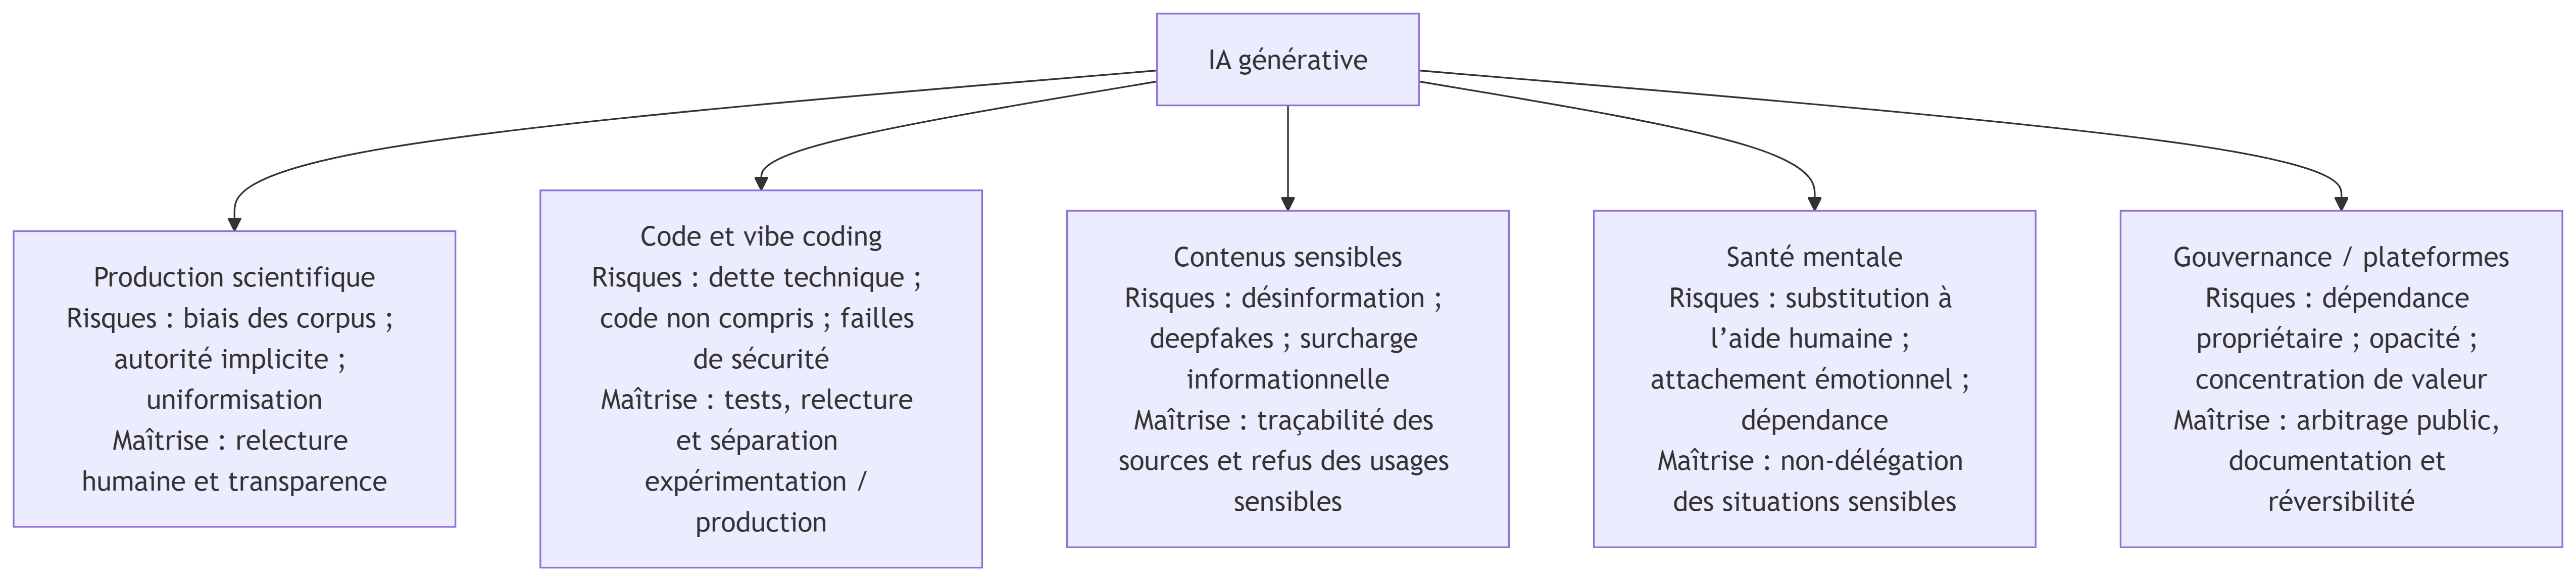
\includegraphics[width=9in,height=8in]{impact_IA_files/figure-latex/mermaid-figure-1.png}

Résumé des risques sociaux de l'IA générative

\section{Travail humain invisible derrière
l'IA}\label{travail-humain-invisible-derriuxe8re-lia}

\subsection{Annotation, modération et évaluation
humaine}\label{annotation-moduxe9ration-et-uxe9valuation-humaine}

Le premier risque est celui du \textbf{travail invisible}. Les modèles
d'IA ne sont pas seulement le résultat d'algorithmes et de calculs : ils
reposent aussi sur du travail humain, parfois peu visible, pour
l'annotation de données, le classement de réponses, l'évaluation de la
qualité ou la modération de contenus. Une enquête de \emph{TIME} a
montré qu'OpenAI avait eu recours à des travailleurs kényans, via un
sous-traitant (Sama), pour identifier des contenus toxiques utilisés
dans l'amélioration de ChatGPT, avec des rémunérations souvent
inférieures à \textbf{2 \$ par heure} et une exposition à des contenus
violents ou traumatisants. Le \emph{Guardian} a également documenté les
conséquences psychologiques de ce type de travail.

Cette dimension humanitaire rappelle que l'IA peut déplacer une partie
de la charge mentale ou du travail pénible vers des personnes peu
visibles, souvent situées dans des pays où le coût du travail est plus
bas. L'utilisateur final voit une interface fluide et rapide, pas
nécessairement les conditions sociales qui ont rendu possible
l'entraînement, le filtrage et l'amélioration des modèles.

Dans CleanMyMap, cette réalité conduit à une règle simple : l'IA ne doit
pas être utilisée par réflexe ni à grande échelle sans valeur ajoutée
démontrable. Son usage doit rester ciblé, traçable et proportionné, puis
être réévalué à l'aide de l'IUR et des règles de sobriété du projet.

Au-delà de ce travail invisible, l'IA modifie aussi la valeur perçue de
certaines compétences : des tâches qui demandaient du temps, de
l'expérience ou une expertise deviennent plus rapides, moins rares et
parfois moins bien rémunérées. Ce déplacement peut aider de petites
équipes à produire davantage, mais il peut aussi fragiliser des métiers
créatifs, éditoriaux, techniques ou administratifs dont la valeur
reposait sur une compétence difficile à reproduire.

Pour CleanMyMap, cette tension doit rester explicite. L'IA peut
accélérer un projet étudiant ou associatif, mais elle ne doit pas servir
à invisibiliser davantage le travail humain, à dévaloriser des
contributions créatives, ou à remplacer des expertises sans
consentement, rémunération ou validation. Dans les choix visuels,
éditoriaux ou institutionnels du projet, l'usage d'IA doit donc rester
transparent, relu et subordonné à une intention humaine identifiable.

\subsection{Transformation du travail et perte de
savoir-faire}\label{transformation-du-travail-et-perte-de-savoir-faire}

L'IA ne transforme pas seulement les chaînes de production matérielles ;
elle transforme aussi le travail intellectuel. Des tâches de rédaction,
de code, de design, de traduction, de support ou de recherche
documentaire peuvent être automatisées partiellement, ce qui modifie la
structure des métiers concernés. Cette évolution peut accélérer le
travail, mais elle peut aussi faire pression sur la valeur de certaines
professions et rendre plus difficile la défense de compétences humaines
qui demandaient auparavant du temps, de l'expérience et une pratique
répétée.

Le risque principal n'est pas le remplacement total des métiers, mais
leur décomposition en tâches plus fragmentées : l'humain relit, corrige,
intègre ou valide des propositions déjà produites par l'IA. À force de
déléguer la rédaction, le code ou l'analyse, les utilisateurs peuvent
perdre une partie de leurs réflexes de base : structurer un argument,
diagnostiquer une erreur, relire un texte, estimer la fiabilité d'un
calcul ou comprendre une architecture. La productivité apparente
augmente, mais la maîtrise réelle peut diminuer si l'outil remplace trop
vite l'apprentissage.

Cette évolution rejoint ce que l'on observe dans les métiers créatifs :
l'IA peut produire quelque chose de visuellement correct ou fonctionnel,
mais cela ne suffit pas à remplacer l'intention, le choix, l'angle et la
responsabilité de la personne qui crée. Dans l'image, le texte ou la
mise en forme, ce qui compte n'est pas seulement le résultat final, mais
aussi le sens du geste, le contexte de production et l'accord de ceux
dont le travail a pu servir de base. Le risque n'est donc pas uniquement
économique ; il est aussi symbolique, quand le travail humain devient
moins visible, moins reconnu ou trop facilement imitable.

Pour CleanMyMap, cette question est stratégique. Le projet a besoin de
personnes capables de comprendre ce qu'il fait, pas seulement de le
faire fonctionner par délégation. L'IA peut accélérer l'itération, mais
elle ne doit pas déqualifier l'équipe au point de rendre le projet
opaque à ceux qui le portent. La bonne règle est donc de garder l'humain
au centre des décisions et de n'utiliser l'IA que comme un soutien
réversible, explicable et contrôlé.

\subsection{Externalisation et conditions de
travail}\label{externalisation-et-conditions-de-travail}

Le développement des grands modèles de langage ne repose pas seulement
sur des ingénieurs, des GPU et des data centers. Il dépend aussi d'un
important travail humain d'annotation, de classement, de vérification,
de filtrage et de modération. Une partie de ce travail est externalisée
vers des prestataires spécialisés ou des plateformes de microtravail,
comme \textbf{Sama}, \textbf{Scale AI}, \textbf{Remotasks} ou d'autres
intermédiaires. Ces tâches peuvent consister à évaluer des réponses,
corriger des sorties, classer des images, signaler des contenus
toxiques, annoter des données ou entraîner les modèles à refuser
certaines demandes.

Ce travail reste souvent peu visible pour l'utilisateur final.
L'interface donne l'impression d'un service automatisé, fluide et
instantané, alors qu'une partie de sa qualité dépend d'une chaîne de
sous-traitance humaine. Des enquêtes ont documenté des situations
préoccupantes, notamment au Kenya, où des travailleurs employés via Sama
pour des tâches liées à OpenAI ont été exposés à des contenus très
violents ou traumatisants, avec des rémunérations inférieures à
\textbf{2 \$ de l'heure} selon l'enquête du \emph{TIME}
(\citeproc{ref-time_openai_used}{TIME, n.d.-a}). Des controverses
comparables ont aussi concerné la modération de contenus pour Meta via
Sama, avec des accusations de bas salaires, de conditions psychologiques
difficiles et de protection insuffisante des travailleurs
(\citeproc{ref-associated_press_the}{T, n.d.}).

Les Philippines constituent un autre exemple important de cette économie
invisible. Des enquêtes sur les travailleurs de l'annotation montrent
que des plateformes liées à l'entraînement de systèmes d'IA, notamment
\textbf{Remotasks} et \textbf{Scale AI}, mobilisent des travailleurs
payés à la tâche, parfois depuis des cybercafés ou dans des conditions
précaires. Ces personnes effectuent des tâches indispensables au
fonctionnement des modèles : annotation d'images, correction de données,
évaluation de réponses, classement de contenus ou préparation de jeux de
données. Le travail est présenté comme flexible, mais il peut aussi être
instable, mal rémunéré, peu protégé et dépendant d'intermédiaires
difficilement contestables (\citeproc{ref-etui_the_filipino}{ETUI,
n.d.}).

Cette réalité crée une contradiction directe pour CleanMyMap. Les outils
utilisés pour accélérer le développement du site, produire du code ou
structurer le rapport reposent en partie sur une chaîne de valeur
mondiale dont les conditions sociales peuvent être éloignées des
principes de responsabilité que le projet entend défendre. L'enjeu n'est
pas de refuser toute IA par principe, mais de reconnaître que son coût
social ne se limite pas au développeur qui l'utilise ni au fournisseur
qui l'héberge. Il inclut aussi des travailleurs souvent invisibles,
situés dans des marchés du travail moins protégés, qui participent à
rendre ces modèles utilisables, sûrs et commercialement acceptables.

Pour CleanMyMap, cette analyse impose une règle de proportion : l'IA ne
doit pas être utilisée comme un réflexe de confort ou de production
illimitée. Elle doit être réservée aux tâches où sa valeur ajoutée est
réelle : gain de qualité, réduction d'erreurs, meilleure documentation,
amélioration de l'accessibilité, accélération d'un service utile ou
renforcement de la sobriété du projet. À l'inverse, les usages
décoratifs, redondants, massifs ou faiblement utiles doivent être
évités, car ils ajoutent de la demande à une industrie dont les coûts
humains restent partiellement externalisés.

\subsection{Risques psychologiques liés à la
modération}\label{risques-psychologiques-liuxe9s-uxe0-la-moduxe9ration}

Le travail invisible lié à l'IA ne se limite pas aux tâches techniques
d'annotation ou de classement. Il comprend aussi une part plus difficile
à soutenir humainement : la \textbf{modération de contenus violents,
haineux, sexuels ou traumatisants} utilisés pour entraîner, filtrer ou
sécuriser les modèles. Pour rendre un modèle plus sûr, des travailleurs
doivent parfois lire, regarder, classer ou signaler des contenus
extrêmes afin d'apprendre au système à les reconnaître et à les refuser.

Cette exposition répétée peut provoquer des conséquences psychologiques
importantes. Des enquêtes journalistiques, notamment celles du
\emph{Guardian} et du \emph{TIME}, ont documenté des situations où des
modérateurs employés par des sous-traitants de grandes entreprises
technologiques ont été confrontés pendant des heures à des contenus de
violence, d'abus, de haine ou d'exploitation sexuelle. Plusieurs travaux
et témoignages évoquent des symptômes proches du \textbf{trouble de
stress post-traumatique}, comme des cauchemars, de l'anxiété, une
désensibilisation, une détresse émotionnelle ou des difficultés à se
détacher des images consultées.

Les fournisseurs et leurs sous-traitants mettent parfois en avant des
dispositifs de soutien psychologique, mais les enquêtes suggèrent que
leur accès réel peut rester insuffisant, en particulier pour les
travailleurs externalisés, précaires ou situés loin des pays
commanditaires. Le problème n'est donc pas seulement l'existence d'un
soutien théorique, mais sa qualité, sa durée, son accessibilité et sa
capacité à protéger réellement les personnes exposées.

Ce risque doit être intégré à un rapport d'impact honnête. L'utilisateur
final voit une interface fluide, propre et apparemment automatisée, mais
cette sécurité apparente repose en partie sur des personnes qui ont
absorbé une partie de la violence du web pour entraîner les modèles à la
filtrer. L'impact social de l'IA ne se limite donc pas à l'énergie, au
carbone ou aux data centers : il inclut aussi une chaîne humaine de
modération, souvent externalisée et peu visible.

Pour CleanMyMap, cette réalité impose une règle de sobriété sociale. Il
ne s'agit pas de considérer que chaque requête individuelle produit
directement un traumatisme, mais de reconnaître que l'usage massif des
modèles participe à financer et entretenir une industrie dont une partie
de la sécurité repose sur ce travail humain difficile. Le projet doit
donc éviter les appels IA inutiles, les boucles de génération excessives
et les usages décoratifs. Chaque usage de l'IA doit être réévalué
régulièrement : il n'est justifiable que s'il apporte une utilité claire
au développement, à la qualité du site, à l'accessibilité, à la sécurité
ou à l'action terrain.

\chapter{Partie IV --- Pouvoir, infrastructures et souveraineté
numérique}\label{partie-iv-pouvoir-infrastructures-et-souverainete-numerique}

Cette partie analyse l'IA comme un système industriel et géopolitique :
elle ne dépend pas seulement de modèles logiciels, mais aussi
d'infrastructures matérielles, de plateformes privées, de chaînes
d'approvisionnement et de rapports de pouvoir internationaux.

\section{Infrastructures critiques de
l'IA}\label{infrastructures-critiques-de-lia}

\subsection{Dépendance aux modèles
propriétaires}\label{duxe9pendance-aux-moduxe8les-propriuxe9taires}

Le premier risque est celui de la \textbf{dépendance aux modèles
propriétaires}. Dans CleanMyMap, plusieurs services externes sont
mobilisés : \textbf{OpenAI} pour l'IA, \textbf{Vercel} pour
l'hébergement, \textbf{Supabase} pour la base de données et le stockage,
\textbf{Clerk} pour l'authentification, \textbf{Resend} pour les emails,
\textbf{PostHog} pour l'analyse d'usage et \textbf{Sentry} pour le suivi
des erreurs. Ces outils permettent de développer plus vite, avec moins
d'infrastructure à maintenir soi-même, mais ils créent aussi une
dépendance technique, économique et organisationnelle.

Cette dépendance peut fragiliser le projet de plusieurs manières :
hausse de prix, changement de quotas, modification des conditions
d'utilisation, panne, fermeture de compte, restriction d'accès,
changement d'API ou évolution juridique. Le risque n'est donc pas
seulement technique. Il concerne aussi la capacité du projet à rester
autonome, compréhensible et maintenable si un fournisseur devient trop
coûteux, indisponible ou incompatible avec les besoins de CleanMyMap.

Cette situation s'inscrit dans un mouvement plus large de
\textbf{centralisation technologique}. Le marché mondial de
l'infrastructure cloud est dominé par un petit nombre d'acteurs. Selon
Synergy Research Group, \textbf{Amazon, Microsoft et Google}
représentaient ensemble environ \textbf{63 \%} des dépenses mondiales
d'infrastructure cloud au troisième trimestre 2025. Cette concentration
pose des questions de souveraineté numérique, de pouvoir de négociation,
de disponibilité des services, de conformité juridique et de dépendance
aux infrastructures extra-européennes.

Dans CleanMyMap, le point de dépendance le plus structurant est le
triptyque \textbf{Vercel + Supabase + Clerk}, qui concentre
l'hébergement, les données et l'identité. Si l'un de ces services
devient indisponible ou difficile à remplacer, le cœur du service peut
être affecté : connexion des utilisateurs, accès aux données, stockage
des photos, API, déploiement ou gestion des rôles. D'autres dépendances
deviennent sensibles si elles passent du statut d'outil auxiliaire à
celui de condition de fonctionnement : \textbf{OpenAI},
\textbf{Pinecone}, \textbf{Google Sheets}, \textbf{PostHog},
\textbf{Upstash}, \textbf{Sentry}, \textbf{Resend} ou \textbf{Stripe}.

L'enjeu n'est pas de refuser toute externalisation. Pour un projet
étudiant, associatif ou citoyen, utiliser des services gérés peut être
plus réaliste, plus sûr et plus sobre que maintenir soi-même une
infrastructure complexe. Le problème apparaît lorsque la pile technique
devient si fermée ou si imbriquée qu'une hausse de prix, une coupure, un
changement d'API ou une contrainte juridique suffit à bloquer le projet.

La réponse de gouvernance consiste donc à limiter les dépendances
critiques et à préparer leur réversibilité. CleanMyMap doit conserver
des formats d'export simples, documenter les services essentiels, éviter
de rendre l'IA indispensable au fonctionnement du site, maintenir des
fonctions centrales compréhensibles sans fournisseur unique, et prévoir
des modes dégradés lorsque c'est possible. Les fonctions utiles au
terrain --- signaler, localiser, organiser, documenter et exporter ---
doivent rester prioritaires et remplaçables.

Cette vigilance vaut particulièrement pour l'IA. Une fonctionnalité IA
ne doit pas devenir une brique centrale si une règle simple, une
validation humaine ou un algorithme déterministe suffit. Plus une
dépendance est puissante, opaque ou difficile à auditer, plus son usage
doit être limité, mesuré et désactivable. Dans CleanMyMap, l'autonomie
ne signifie donc pas l'absence totale de services externes, mais la
capacité à comprendre, réduire, remplacer ou couper une dépendance avant
qu'elle ne devienne un point de blocage.

\subsection{Dépendance aux clouds, API et services
externes}\label{duxe9pendance-aux-clouds-api-et-services-externes}

La centralisation de l'IA est structurelle à trois niveaux. Le premier
niveau est celui de l'\textbf{infrastructure cloud} : AWS, Microsoft
Azure et Google Cloud concentrent environ \textbf{63 \%} des dépenses
mondiales d'infrastructure cloud au troisième trimestre 2025. Le
deuxième niveau est celui des \textbf{modèles fondationnels} : une
poignée de laboratoires, notamment OpenAI, Anthropic, Google DeepMind,
Meta, xAI, Mistral ou DeepSeek, contrôle l'accès aux modèles les plus
performants, aux API, aux outils de code et aux grands contextes. Le
troisième niveau est celui des \textbf{semi-conducteurs} : NVIDIA domine
encore largement le marché des GPU et accélérateurs utilisés pour
l'entraînement et l'inférence IA, avec des estimations souvent situées
entre \textbf{70 \% et 90 \%} du marché selon le périmètre retenu.

Cette triple concentration crée une fragilité systémique. Une panne chez
un grand fournisseur cloud, une hausse brutale des prix, une restriction
d'accès à une API, une tension géopolitique sur les puces ou une rupture
d'approvisionnement peut affecter simultanément des milliers de
services. Le risque n'est donc pas seulement celui d'un fournisseur
isolé, mais celui d'un écosystème entier dépendant des mêmes
infrastructures, des mêmes modèles, des mêmes GPU et parfois des mêmes
régions cloud.

Cette dépendance est renforcée par les effets de verrouillage. Dans le
cloud, les applications utilisent souvent des services spécifiques
difficiles à remplacer rapidement. Pour les modèles, les développeurs
s'habituent à une API, à une qualité de réponse, à un format de sortie
ou à un outil de code particulier. Pour les puces, l'écosystème NVIDIA
est renforcé par CUDA, les bibliothèques logicielles, les frameworks
optimisés et la disponibilité des compétences. Plus ces couches
deviennent intégrées, plus le coût de sortie augmente.

Pour CleanMyMap, la conséquence pratique est claire : l'IA ne doit pas
devenir une brique indispensable du service. Le projet doit pouvoir
continuer à remplir ses fonctions centrales --- signaler, localiser,
organiser, documenter et exporter --- même si un fournisseur IA devient
indisponible ou trop coûteux. Les opérations critiques doivent donc
rester fondées sur des mécanismes simples, auditables et remplaçables :
base de données exportable, formats standards, fonctions désactivables,
documentation technique, modes dégradés et limitation des appels à des
services propriétaires.

Cette stratégie ne suppose pas de refuser les grands fournisseurs. Elle
consiste plutôt à éviter une dépendance excessive. Les outils cloud, les
modèles puissants et les GPU spécialisés peuvent être utiles pour
développer plus vite ou améliorer la qualité du service, mais ils
doivent rester proportionnés à l'utilité réelle du projet. Dans
CleanMyMap, la souveraineté technique ne signifie pas tout héberger
soi-même ; elle signifie conserver la capacité de comprendre, réduire,
remplacer ou couper une dépendance avant qu'elle ne bloque le cœur du
service.

\section{Concentration économique et pouvoir des
plateformes}\label{concentration-uxe9conomique-et-pouvoir-des-plateformes}

\subsection{Centralisation du cloud, des modèles et des
puces}\label{centralisation-du-cloud-des-moduxe8les-et-des-puces}

La centralisation de l'IA est structurelle à trois niveaux. Le premier
niveau est celui de l'\textbf{infrastructure cloud} : AWS, Microsoft
Azure et Google Cloud concentrent environ \textbf{63 \%} des dépenses
mondiales d'infrastructure cloud au troisième trimestre 2025. Le
deuxième niveau est celui des \textbf{modèles fondationnels} : une
poignée de laboratoires, notamment OpenAI, Anthropic, Google DeepMind,
Meta, xAI, Mistral ou DeepSeek, contrôle l'accès aux modèles les plus
performants, aux API, aux outils de code et aux grands contextes. Le
troisième niveau est celui des \textbf{semi-conducteurs} : NVIDIA domine
encore largement le marché des GPU et accélérateurs utilisés pour
l'entraînement et l'inférence IA, avec des estimations souvent situées
entre \textbf{70 \% et 90 \%} du marché selon le périmètre retenu.

\subsection{Concentration de la valeur autour de quelques
acteurs}\label{concentration-de-la-valeur-autour-de-quelques-acteurs}

Le développement de l'IA s'accompagne d'une forte \textbf{concentration
économique de la valeur}. En 2024-2025, les entreprises les mieux
valorisées au monde --- \textbf{Microsoft, NVIDIA, Alphabet, Meta et
Amazon} --- sont toutes liées directement ou indirectement à l'essor de
l'IA : cloud, modèles fondationnels, puces, publicité, données,
infrastructures ou plateformes de distribution. L'exemple le plus
visible est \textbf{NVIDIA}, dont la capitalisation boursière a dépassé
les \textbf{3 000 milliards de dollars} en juin 2024, portée par la
demande mondiale en GPU nécessaires à l'entraînement et à l'inférence
des modèles d'IA. Reuters indiquait également que NVIDIA était devenue,
en juin 2024, l'entreprise la plus valorisée au monde, devant Microsoft
et Apple, ce qui illustre le rôle central des puces IA dans la nouvelle
économie numérique.

\subsection{Corpus, consentement et rémunération des
créateurs}\label{corpus-consentement-et-ruxe9munuxe9ration-des-cruxe9ateurs}

L'essor des modèles fondationnels repose aussi sur l'utilisation massive
de corpus d'œuvres, de textes, d'images, de code, de musiques et
d'articles souvent collectés à grande échelle, sans consentement clair
ni rémunération proportionnelle des auteurs. Cette situation alimente
une critique de plus en plus structurée : la valeur créée par les
créateurs est captée en amont par l'entraînement, puis monétisée en aval
par des services d'IA capables de résumer, reformuler ou concurrencer
ces mêmes productions.

Le problème n'est pas seulement juridique. Il est aussi économique et
culturel. Lorsque des créations humaines deviennent de la matière
d'entraînement peu visible, les bénéfices se concentrent chez les
fournisseurs de modèles, de cloud, de puces et de plateformes, tandis
que les coûts de production initiale, d'originalité et de travail
créatif sont diffusés, parfois sans contrepartie claire. Cela pose une
question de justice pour les auteurs, les journalistes, les artistes,
les développeurs et plus largement pour toute la chaîne de production
culturelle.

Pour CleanMyMap, la conséquence pratique est simple : le projet doit
documenter les outils utilisés, privilégier autant que possible des
services dont les règles de collecte et d'utilisation des données sont
explicites, et éviter d'entretenir l'idée qu'un service d'IA n'a pas de
coût parce qu'il serait ``gratuit''. Même lorsqu'un outil semble libre
d'accès, il repose sur une infrastructure et sur des corpus qui ont une
valeur économique réelle. Une gouvernance responsable doit donc regarder
la provenance des modèles, leur politique de données et leur mode de
financement avec autant d'attention que leurs performances techniques.

\subsection{IA et colonialisme
numérique}\label{ia-et-colonialisme-numuxe9rique}

Au-delà du débat sur le consentement, l'IA peut aussi être lue comme un
phénomène de \textbf{colonialisme numérique}. Les données, le travail
d'annotation, les contenus culturels, la puissance de calcul et les
ressources matérielles sont extraits à l'échelle mondiale, mais la
valeur économique, la propriété des modèles et une grande partie de la
capacité de décision restent concentrées chez quelques entreprises du
Nord global.

Cette asymétrie rappelle une logique d'extraction : des territoires, des
langues et des communautés alimentent l'écosystème IA, tandis que les
bénéfices majeurs remontent vers les acteurs qui contrôlent les modèles,
le cloud, les puces ou les plateformes. Le rapport de force est alors
déséquilibré non seulement dans les prix, mais aussi dans la capacité à
fixer les règles, à orienter les usages et à capter les retombées.

Pour CleanMyMap, cette lecture impose une prudence accrue : documenter
l'origine des services utilisés, réduire la dépendance aux
intermédiaires non essentiels, préférer des outils dont les conditions
d'usage sont transparentes et éviter de reproduire, à son échelle, une
logique d'extraction invisible. Une technologie utile n'est pas
automatiquement une technologie juste ; elle doit aussi être gouvernée
de manière explicite et proportionnée.

\subsection{Effets de domination sur les développeurs, entreprises et
institutions}\label{effets-de-domination-sur-les-duxe9veloppeurs-entreprises-et-institutions}

Cette concentration ne vient pas seulement de la performance technique
des entreprises concernées. Elle repose aussi sur des \textbf{barrières
d'entrée très élevées} : coût des data centers, accès aux GPU, capacité
à acheter de l'électricité à grande échelle, volume de données
disponibles, maîtrise du cloud, intégration logicielle, brevets,
écosystèmes propriétaires et capacité financière à entraîner des modèles
de plus en plus coûteux. Le cloud illustre déjà cette tendance : selon
Synergy Research Group, \textbf{Amazon, Microsoft et Google}
représentaient ensemble environ \textbf{63 \%} des dépenses mondiales
d'infrastructure cloud au troisième trimestre 2025.

L'émergence de modèles comme DeepSeek suggère toutefois que les
centaines de milliards investis dans une logique de \textbf{brute force
computationnelle} ne constituent peut-être pas un avantage concurrentiel
durable, mais potentiellement un piège économique et énergétique : des
architectures plus sobres, moins dépendantes de l'accumulation massive
de GPU et optimisées pour l'efficacité pourraient progressivement
remettre en cause la domination historique de certains acteurs de la
Silicon Valley, comme les premières réactions des marchés lors de
l'émergence de DeepSeek semblent déjà l'avoir partiellement montré.
Cette lecture doit rester prudente, mais elle indique qu'une partie de
la compétition IA pourrait se déplacer de la puissance brute vers
l'efficacité d'inférence, la sobriété matérielle et le rapport
coût/performance.

Voici la conclusion très évocatrice de la vidéo \emph{La CHINE a libéré
un MONSTRE : DeepSeek V4} : ``Les Américains vont plus vite, les Chinois
sont plus légers. La question ce n'est pas qui est devant aujourd'hui
mais quel modèle est le plus durable. La prochaine fois qu'un
laboratoire Américain annoncera 100 milliards d'investissement
posez-vous la question : est-ce une démonstration de force, ou l'aveu
que la force ne suffit plus?''

Les gains économiques directs --- abonnements, API, cloud, vente de GPU,
hausse de productivité, valorisation boursière --- bénéficient
principalement aux grandes plateformes, à leurs actionnaires et aux
entreprises capables d'intégrer rapidement l'IA. En revanche, une partie
des coûts est largement mutualisée : consommation électrique, pression
sur l'eau, extraction de matériaux, déchets électroniques, travail
invisible d'annotation et de modération, dépendance technologique,
fragilisation de certains métiers et ajustements d'emploi liés à
l'automatisation.

Le risque n'est donc pas seulement environnemental ou technique. Il est
aussi social et politique. L'IA peut accroître la productivité, mais
cette productivité ne se traduit pas automatiquement par une répartition
équitable de la valeur. Elle peut au contraire renforcer des positions
dominantes, déplacer du travail humain vers des sous-traitants peu
visibles, réduire le pouvoir de négociation de certains travailleurs et
rendre de nombreux projets dépendants de services contrôlés par quelques
entreprises mondiales.

Les fonds consacrés au développement de \textbf{CleanMyMap} participent
aussi à un système économique très concentré, dans lequel les bénéfices
financiers et les coûts sociaux ne sont pas répartis de manière
symétrique.

\subsection{Fragilité d'un écosystème dépendant de plateformes
privées}\label{fragilituxe9-dun-uxe9cosystuxe8me-duxe9pendant-de-plateformes-privuxe9es}

La réponse de CleanMyMap ne peut donc pas être de présenter l'IA comme
un outil neutre ou automatiquement émancipateur. Elle consiste plutôt à
en limiter l'usage aux cas où la valeur ajoutée est démontrée, à
conserver une gouvernance humaine, à éviter les dépendances inutiles, à
documenter les fournisseurs utilisés et à maintenir une architecture
aussi réversible que possible. L'IA reste acceptable si elle sert une
utilité environnementale ou sociale réelle ; elle devient problématique
si elle renforce surtout la dépendance à des plateformes déjà dominantes
sans bénéfice terrain proportionné.

\section{Souveraineté numérique et géopolitique de
l'IA}\label{souverainetuxe9-numuxe9rique-et-guxe9opolitique-de-lia}

\subsection{Dépendance européenne aux infrastructures
étrangères}\label{duxe9pendance-europuxe9enne-aux-infrastructures-uxe9tranguxe8res}

La dépendance aux infrastructures cloud, aux modèles d'IA et aux
fournisseurs américains soulève des questions croissantes de
\textbf{souveraineté numérique} en Europe. Le RGPD impose un cadre
strict sur la collecte, le traitement, le stockage et le transfert des
données personnelles, notamment lorsqu'elles sortent de l'Union
européenne. Or les API d'IA grand public ou professionnelles peuvent
impliquer l'envoi de instructions, de fichiers, de logs ou d'extraits de
code vers des infrastructures dont la localisation exacte, la durée de
conservation ou les sous-traitants ne sont pas toujours clairement
maîtrisés par l'utilisateur final.

Le risque ne concerne pas seulement les données personnelles explicites.
Un instruction peut contenir des informations sensibles sans que
l'utilisateur s'en rende compte : architecture technique, erreurs
serveur, extraits de base de données, noms d'utilisateurs, coordonnées,
clés mal masquées, logs, informations métier ou éléments stratégiques du
projet. Dans un projet comme CleanMyMap, qui peut traiter des
signalements localisés, des photos, des comptes utilisateurs, des
données associatives ou des échanges institutionnels, cette vigilance
est indispensable. L'usage d'une IA externe doit donc être encadré par
une règle simple : ne transmettre que le strict nécessaire, anonymiser
ce qui peut l'être, exclure les secrets techniques et éviter tout envoi
de données personnelles non indispensables.

\subsection{Semi-conducteurs, restrictions d'exportation et compétition
industrielle}\label{semi-conducteurs-restrictions-dexportation-et-compuxe9tition-industrielle}

La souveraineté numérique est aussi un enjeu géopolitique. La chaîne de
valeur de l'IA dépend d'un petit nombre d'acteurs et de territoires :
fournisseurs cloud américains, laboratoires de modèles, fabricants de
GPU, chaînes d'assemblage, fonderies avancées et matières premières
critiques. La concentration de la production de puces avancées autour de
TSMC à Taïwan, souvent estimée autour de \textbf{90 \%} pour les nœuds
les plus avancés, illustre cette fragilité. Les restrictions
d'exportation américaines sur certains GPU et technologies de calcul
montrent également que l'IA est devenue un instrument stratégique entre
grandes puissances, et non un simple marché logiciel.

\subsection{Tensions entre innovation, souveraineté et sécurité
nationale}\label{tensions-entre-innovation-souverainetuxe9-et-suxe9curituxe9-nationale}

Cette situation crée une dépendance indirecte pour tous les projets
utilisant l'IA, même modestement. CleanMyMap ne contrôle ni la
production des puces, ni les politiques d'exportation, ni les choix
d'infrastructure des grands fournisseurs. En revanche, le projet peut
réduire sa vulnérabilité en documentant ses dépendances, en distinguant
les services critiques des services optionnels, en conservant des
exports de données, en limitant les appels IA et en évitant de rendre
une API propriétaire indispensable au fonctionnement du site.

Pour CleanMyMap, la recommandation opérationnelle est donc triple.
Premièrement, documenter les services utilisés : fournisseur, rôle,
données traitées, région d'hébergement si connue, criticité et
possibilité de désactivation. Deuxièmement, vérifier la conformité RGPD
des usages IA : instructions sans données personnelles inutiles, absence
de secrets, anonymisation des logs, information des utilisateurs lorsque
c'est nécessaire. Troisièmement, anticiper des scénarios de migration ou
de réduction de dépendance vers des fournisseurs européens, source
ouverte ou plus facilement remplaçables si les conditions
réglementaires, économiques ou géopolitiques évoluent.

L'objectif n'est pas de prétendre à une souveraineté totale, irréaliste
pour un projet étudiant ou associatif. Il est plus raisonnable de viser
une \textbf{souveraineté fonctionnelle} : savoir où sont les
dépendances, comprendre ce qu'elles font, pouvoir exporter les données,
couper les fonctions non essentielles et maintenir le cœur du service
même si un fournisseur devient indisponible, trop coûteux ou
juridiquement problématique.

\subsection{Modèles ouverts, modèles propriétaires et autonomie
stratégique}\label{moduxe8les-ouverts-moduxe8les-propriuxe9taires-et-autonomie-stratuxe9gique}

Les modèles ouverts ou open-weight réduisent une partie du verrouillage,
mais ils ne suppriment pas la dépendance matérielle et opérationnelle.
Un modèle comme DeepSeek, Llama, Mistral ou GPT-OSS peut être plus
facilement auditable, auto-hébergeable ou remplaçable qu'une API fermée
; en revanche, il peut continuer à dépendre d'une machine puissante,
d'un GPU coûteux ou d'une infrastructure distante si l'exécution locale
n'est pas réaliste.

Pour CleanMyMap, l'autonomie stratégique ne consiste donc pas à opposer
modèles ouverts et modèles propriétaires de manière idéologique. Elle
consiste à conserver plusieurs options, à documenter les critères de
choix, à privilégier le modèle le plus léger capable de faire
correctement le travail et à éviter qu'un seul fournisseur ne devienne
indispensable. Les modèles ouverts sont utiles s'ils améliorent la
réversibilité, l'auditabilité et la continuité du service ; les modèles
propriétaires restent acceptables s'ils apportent un gain clair sans
verrouiller l'architecture.

\section{Biais, discrimination, inégalités et délégation du
jugement}\label{biais-discrimination-inuxe9galituxe9s-et-duxe9luxe9gation-du-jugement}

\subsection{Biais de données et reproduction des
inégalités}\label{biais-de-donnuxe9es-et-reproduction-des-inuxe9galituxe9s}

Les grands modèles de langage sont entraînés sur des corpus massifs
composés de textes, de code, d'images, de pages web, de forums, de
livres numérisés, de documentation technique et de contenus produits par
des utilisateurs. Ces corpus ne représentent pas le monde de manière
neutre. Ils sont souvent marqués par une surreprésentation des contenus
anglophones, occidentaux, numériquement visibles, issus de milieux
éduqués ou de pays fortement connectés. À l'inverse, les langues
minoritaires, les savoirs locaux, les récits du Sud global, les
expériences populaires ou les formes de connaissance peu présentes en
ligne peuvent être sous-représentés.

Cette composition influence les réponses des modèles. Un modèle ne
comprend pas le monde directement : il apprend des régularités
statistiques à partir des données disponibles. Si ces données
contiennent des stéréotypes, des rapports de domination, des
associations implicites entre certains groupes et certaines situations
sociales, le modèle peut les reproduire ou les renforcer. C'est l'un des
enjeux soulignés par Bender et al.~dans \emph{Stochastic Parrots} : un
modèle peut produire un langage fluide et crédible tout en reflétant les
biais, angles morts et rapports de pouvoir présents dans ses corpus
d'entraînement.

Ces biais ne sont pas seulement théoriques. Les travaux de Buolamwini et
Gebru dans \emph{Gender Shades} ont montré que des systèmes de
classification faciale présentaient des taux d'erreur très différents
selon le genre et la couleur de peau, avec des performances nettement
moins bonnes pour les femmes à la peau foncée que pour les hommes à la
peau claire (\citeproc{ref-buolamwini_j_et}{Buolamwini, n.d.}). Même si
cette étude porte sur la vision par ordinateur plutôt que sur les
modèles de langage, elle illustre un principe général : lorsqu'un
système d'IA est entraîné sur des données déséquilibrées, il peut
produire des erreurs systématiques dans des applications réelles.

Pour CleanMyMap, les biais les plus pertinents concernent la description
des déchets, des lieux et des territoires. Un modèle pourrait
interpréter différemment une photo, un signalement ou une description
selon le contexte implicite : quartier populaire ou touristique, zone
urbaine dense ou rurale, langage formel ou familier, français standard
ou expressions locales. Il pourrait aussi associer abusivement certains
territoires à la saleté, à l'incivilité ou au manque de civisme, alors
que la présence de déchets dépend souvent de facteurs structurels :
densité de passage, organisation de la collecte, manque d'équipements
publics, événements locaux, activité commerciale, tourisme ou politiques
municipales.

Le risque serait donc de transformer un outil environnemental en outil
de stigmatisation. Une carte des déchets peut être utile pour agir, mais
elle peut aussi produire une image injuste d'un quartier si les données
sont incomplètes, mal modérées ou interprétées sans contexte. De même,
une IA de classification pourrait simplifier abusivement une situation :
confondre un dépôt sauvage avec un point de collecte saturé, interpréter
une photo hors contexte, ou attribuer implicitement une responsabilité
sociale à des habitants plutôt qu'à un défaut d'infrastructure.

Cette prudence vaut aussi pour les contenus créatifs ou visuels utilisés
autour du projet. Un résultat généré peut être séduisant sans pour
autant porter la même intention qu'une création humaine ; il peut même
reproduire des styles reconnaissables sans consentement explicite, ce
qui fragilise à la fois l'éthique et la confiance. Si CleanMyMap utilise
des images, des illustrations ou des supports éditoriaux produits avec
assistance IA, la provenance doit rester claire et la validation humaine
explicite.

Pour cette raison, CleanMyMap ne doit pas utiliser l'IA pour produire
des jugements automatiques sur les territoires, les habitants ou les
comportements. Les modèles peuvent aider à reformuler un signalement,
repérer une incohérence ou assister une modération, mais ils ne doivent
pas décider seuls de la gravité d'une situation, de la responsabilité
d'un acteur ou de la valeur d'un quartier. Les données doivent rester
contextualisées, vérifiables et relues humainement.

La recommandation opérationnelle est donc la suivante : limiter l'IA aux
tâches d'assistance, éviter les scores opaques, documenter les limites
des données, permettre la correction humaine, et ne jamais présenter une
sortie de modèle comme une vérité sociale ou territoriale. Pour
CleanMyMap, un signalement doit rester une information à vérifier et à
replacer dans son contexte, pas une preuve automatique de comportement
collectif.

\subsection{Autorité implicite et normative des réponses
générées}\label{autorituxe9-implicite-et-normative-des-ruxe9ponses-guxe9nuxe9ruxe9es}

La forme fluide, structurée et encyclopédique des réponses produites par
un grand modèle de langage crée une \textbf{autorité implicite}. Le
modèle ne se contente pas de répondre : il hiérarchise, reformule,
conseille, parfois filtre ou contourne certaines formulations, et
oriente subtilement la perception de ce qui semble vrai, normal ou
souhaitable. Il donne ainsi l'impression d'avoir vérifié l'information,
alors qu'il ne fonctionne pas comme une source documentaire classique.
Il génère une réponse probable à partir de ses données d'entraînement,
du contexte fourni et des instructions reçues.

La différence avec un moteur de recherche est importante. Un moteur de
recherche affiche généralement une liste de pages que l'utilisateur peut
comparer, hiérarchiser et vérifier. Un modèle de langage, lui,
\textbf{synthétise directement} une réponse et lui donne une forme
normative implicite : certains mots deviennent plus plausibles,
certaines hypothèses plus naturelles, certains arbitrages plus
raisonnables. Cette synthèse peut donner l'impression que le travail
critique a déjà été fait, alors qu'il reste à contrôler. Le risque est
donc de confondre une réponse bien formulée avec une réponse fiable.
Plus le texte est clair, professionnel et convaincant, plus
l'utilisateur peut être tenté de lui accorder une confiance excessive
(\citeproc{ref-bender_e_m_1}{Bender, n.d.-a};
\citeproc{ref-nist_artificial_intelligence_1}{NIST, n.d.-a}).

Cette autorité implicite est particulièrement problématique dans un
contexte académique, institutionnel ou décisionnel. Une estimation
chiffrée, une référence scientifique, une recommandation technique ou
une conclusion environnementale produite avec l'aide d'un modèle peut
être reprise trop vite dans un rapport, une soutenance ou une décision
de projet. Le danger n'est pas seulement l'hallucination évidente, mais
aussi l'\textbf{erreur plausible} : une source réelle mais mal
interprétée, un chiffre sorti de son contexte, une généralisation
abusive ou une formulation trop catégorique
(\citeproc{ref-openai_gpt_4}{OpenAI, n.d.-d};
\citeproc{ref-nist_artificial_intelligence_1}{NIST, n.d.-a}).

Pour CleanMyMap, ce risque concerne directement les estimations
environnementales, les comparaisons énergétiques, les hypothèses de
consommation d'eau, les références à l'ACV, les analyses sociales, les
recommandations de cybersécurité et les choix techniques. Une phrase
produite par IA ne doit pas être considérée comme vérifiée parce qu'elle
est bien écrite. Chaque affirmation chiffrée, datée, scientifique,
juridique, technique ou institutionnelle doit être croisée avec une
source primaire ou une source fiable avant diffusion
(\citeproc{ref-nist_artificial_intelligence_1}{NIST, n.d.-a}).

La règle de gouvernance est donc simple : l'IA peut aider à formuler,
structurer, résumer ou repérer des incohérences, mais elle ne doit pas
être traitée comme une autorité finale. Les chiffres doivent être
vérifiés, les sources ouvertes, les liens testés, les citations
replacées dans leur contexte et les recommandations techniques relues
par un humain. Lorsqu'une information reste incertaine, le rapport doit
le dire explicitement au lieu de transformer une hypothèse en certitude.

Dans CleanMyMap, cette exigence se traduit par une méthode de validation
: distinguer les faits mesurés, les hypothèses déclaratives et les
ordres de grandeur ; indiquer les sources à la fin de chaque section ;
signaler les affirmations non vérifiées ; éviter les formulations trop
absolues ; et conserver une responsabilité humaine sur toute conclusion
publiée. L'objectif n'est pas d'interdire l'assistance IA, mais
d'empêcher qu'une réponse générée devienne une preuve sans contrôle.

\subsection{Inégalités d'accès aux outils, modèles et capacités de
calcul}\label{inuxe9galituxe9s-daccuxe8s-aux-outils-moduxe8les-et-capacituxe9s-de-calcul}

L'accès à l'IA est profondément inégal. Les meilleurs modèles, les
abonnements les plus complets, les GPU, les outils de productivité et
les environnements de développement avancés sont plus facilement
accessibles aux personnes, entreprises et pays déjà favorisés. À
l'inverse, les utilisateurs moins dotés doivent souvent se contenter de
versions bridées, de quotas plus faibles ou d'outils moins performants.

Ces écarts d'accès ne sont pas neutres. Ils accentuent les différences
de productivité, de vitesse d'apprentissage et de capacité à tester des
idées ou à automatiser des tâches. Pour CleanMyMap, cela rappelle qu'un
projet assisté par IA doit rester lisible et réversible, afin de ne pas
dépendre d'un niveau d'outillage que tous les contributeurs ne
pourraient pas reproduire.

\subsection{Risque de délégation excessive du jugement
humain}\label{risque-de-duxe9luxe9gation-excessive-du-jugement-humain}

La facilité d'usage des modèles de langage peut conduire progressivement
à leur déléguer des décisions qui relèvent normalement du
\textbf{jugement humain} : choix d'architecture, arbitrage éditorial,
interprétation de données, évaluation de risques, hiérarchisation des
priorités ou formulation d'une position institutionnelle. Ce glissement
est souvent discret. Au départ, le modèle sert à gagner du temps ;
ensuite, il propose des options ; puis ses propositions deviennent la
base principale de la décision. Le risque n'est donc pas seulement
l'erreur ponctuelle, mais la transformation progressive de l'IA en
autorité de fait.

Dans un projet de développement, ce mécanisme peut affaiblir la maîtrise
technique. Un développeur qui accepte systématiquement les propositions
d'un modèle sans les comprendre peut produire rapidement du code, mais
perdre en capacité d'analyse, de diagnostic et d'architecture. Il
devient alors dépendant de l'outil pour corriger les erreurs que l'outil
lui-même peut avoir introduites. De la même manière, un rédacteur qui
sous-traite toutes ses formulations peut obtenir un texte fluide, mais
perdre progressivement sa voix propre, son sens critique et sa
responsabilité sur ce qui est affirmé.

Ce risque est renforcé par la \textbf{sycophancy}, c'est-à-dire la
tendance d'un modèle à conforter l'utilisateur dans ses croyances, ses
hypothèses ou ses formulations plutôt qu'à les contredire franchement.
Anthropic a documenté ce comportement dans ses travaux sur la
complaisance des modèles, et OpenAI a également reconnu qu'une mise à
jour de ChatGPT avait pu rendre le modèle trop flatteur ou trop aligné
sur les attentes immédiates de l'utilisateur. Dans un rapport, ce
phénomène est dangereux : un modèle peut rendre une idée plus élégante
sans vérifier qu'elle est juste, ou renforcer une hypothèse déjà fragile
au lieu de la remettre en question.

Pour CleanMyMap, cette délégation excessive serait contradictoire avec
l'objectif de responsabilité. Le projet traite de sujets
environnementaux, sociaux, techniques et institutionnels qui nécessitent
des arbitrages humains explicites. L'IA peut aider à formuler, résumer,
structurer, comparer ou repérer des incohérences, mais elle ne doit pas
décider de l'orientation du produit, du niveau de risque acceptable, du
choix d'une dépendance critique, de la stratégie de communication ou de
l'interprétation finale des impacts.

La règle de gouvernance retenue est donc simple : \textbf{l'IA propose,
l'humain décide}. Toute décision importante doit rester compréhensible,
justifiable et assumée par une personne identifiable. Cela vaut pour
l'architecture technique, les choix de dépendances, la sécurité, les
données personnelles, les chiffres environnementaux, les messages
publics, les conclusions institutionnelles et les recommandations
adressées au jury ou aux partenaires.

Concrètement, aucune décision d'architecture, de communication publique
ou d'orientation produit ne doit être déléguée à un modèle sans
relecture et validation humaine documentée. Une proposition IA doit
pouvoir être refusée, corrigée ou simplifiée. Si le modèle produit une
réponse séduisante mais invérifiable, elle doit être traitée comme une
hypothèse de travail, non comme une preuve. Si une décision engage la
sécurité, les données, l'image publique ou la cohérence écologique du
projet, elle doit être relue humainement avant intégration.

Cette discipline protège à la fois la qualité du projet et la compétence
de l'équipe. L'objectif n'est pas d'interdire l'assistance IA, mais
d'éviter qu'elle remplace le raisonnement. CleanMyMap peut utiliser l'IA
comme accélérateur de travail, mais pas comme substitut au jugement, à
la responsabilité ou à l'apprentissage humain.

\subsection{Dépendance cognitive et baisse de l'effort
critique}\label{duxe9pendance-cognitive-et-baisse-de-leffort-critique}

Un autre risque, plus discret, est la \textbf{dépendance cognitive}.
Quand l'IA devient le premier réflexe avant toute réflexion,
l'utilisateur peut commencer à lui demander quoi faire avant même
d'avoir formulé son propre diagnostic. Le problème n'est pas seulement
de gagner du temps, mais de perdre l'habitude d'examiner un problème par
soi-même, de comparer plusieurs options ou d'assumer une part d'effort
critique.

Cette dépendance peut se traduire par une baisse de vigilance : une
formulation proposée est acceptée plus vite, les vérifications
deviennent moins nombreuses, les tests sont moins fréquents et les
alternatives sont moins comparées. Dans un projet technique, cela peut
conduire à une dégradation lente du jugement professionnel et à une
confusion entre assistance et décision. Pour CleanMyMap, la règle doit
rester simple : l'IA peut accélérer l'analyse, mais elle ne doit pas
devenir un réflexe automatique avant toute pensée.

\section{IA, production scientifique et intégrité de la
connaissance}\label{ia-production-scientifique-et-intuxe9grituxe9-de-la-connaissance}

\subsection{Usage croissant des modèles de langage dans les
publications}\label{usage-croissant-des-moduxe8les-de-langage-dans-les-publications}

L'usage de modèles de langage dans la production académique est en forte
croissance depuis 2023. Des études bibliométriques ont montré que
certains mots caractéristiques des sorties de ChatGPT (comme
\emph{delve}, \emph{commendable}, \emph{intricate} en anglais) ont vu
leur fréquence augmenter de façon statistiquement significative dans les
publications scientifiques après novembre 2022. Cette évolution ne
signifie pas que la moitié de la science serait désormais ``écrite par
IA'' : elle montre plutôt que l'IA devient un outil ordinaire de
rédaction, de reformulation et de structuration scientifique.

{\def\LTcaptype{none} % do not increment counter
\begin{longtable}[]{@{}
  >{\raggedright\arraybackslash}p{(\linewidth - 4\tabcolsep) * \real{0.3000}}
  >{\raggedleft\arraybackslash}p{(\linewidth - 4\tabcolsep) * \real{0.4000}}
  >{\raggedright\arraybackslash}p{(\linewidth - 4\tabcolsep) * \real{0.3000}}@{}}
\toprule\noalign{}
\begin{minipage}[b]{\linewidth}\raggedright
Corpus étudié
\end{minipage} & \begin{minipage}[b]{\linewidth}\raggedleft
Estimation d'usage IA
\end{minipage} & \begin{minipage}[b]{\linewidth}\raggedright
Prudence d'interprétation
\end{minipage} \\
\midrule\noalign{}
\endhead
\bottomrule\noalign{}
\endlastfoot
PubMed biomédical 2024 & au moins 13,5 \% des abstracts & borne basse,
méthode par vocabulaire \\
Certains sous-corpus biomédicaux & jusqu'à 40 \% & ne vaut pas pour
toute la science \\
Computer science dans certains corpus 2024 & jusqu'à 17,5 \% & selon
Liang et al., corpus arXiv, bioRxiv et Nature \\
Mathématiques / Nature portfolio & jusqu'à 6,3 \% & usage plus faible
dans ce corpus \\
\end{longtable}
}

Ce tableau ne mesure pas une fraude systématique : il montre surtout que
l'IA devient un outil ordinaire d'écriture scientifique, ce qui impose
plus de transparence, de déclaration d'usage et de responsabilité
humaine.

Une étude publiée dans Science Advances estime qu'au moins 13,5 \% des
abstracts biomédicaux PubMed publiés en 2024 ont été traités avec des
LLM, avec certains sous-corpus pouvant atteindre 40 \%
(\citeproc{ref-kobak_excess_vocabulary_2025}{Kobak et al. 2025}). Liang
et al.~ont par ailleurs estimé que certaines catégories de papiers
scientifiques montraient une présence mesurable de contenu modifié par
LLM, avec jusqu'à 17,5 \% pour la computer science dans certains corpus
et jusqu'à 6,3 \% pour les mathématiques et Nature portfolio
(\citeproc{ref-liang_increasing_use_llms_scientific_papers_2024}{Liang
et al. 2024}). Ces résultats concernent des corpus précis, pas toute la
science mondiale.

Des éditeurs majeurs comme \emph{Nature}, \emph{Science} et Elsevier ont
mis à jour leurs politiques pour exiger la déclaration de tout usage de
modèle de langage dans la rédaction. Ce rapport lui-même a bénéficié
d'une assistance IA pour sa structuration et sa rédaction : cette
réalité est déclarée en préambule et dans la méthodologie.

\subsection{Risque d'uniformisation du style
scientifique}\label{risque-duniformisation-du-style-scientifique}

Si une proportion croissante de publications est rédigée ou co-rédigée
avec des modèles de langage, il existe un risque d'uniformisation
progressive du style académique : convergence vers les formulations
statistiquement préférées par les modèles, appauvrissement de la
diversité rhétorique et homogénéisation des structures argumentatives.

À terme, cela pourrait rendre plus difficile la distinction des voix
individuelles, des approches disciplinaires et des traditions
académiques nationales. Ce risque est encore documenté de façon
exploratoire, mais il s'ajoute à la question de la prédominance des
conventions académiques anglo-saxonnes dans les corpus d'entraînement,
qui peut avantager les formulations proches de celles-ci au détriment
d'autres traditions intellectuelles.

\subsection{Transparence insuffisante sur l'usage de
l'IA}\label{transparence-insuffisante-sur-lusage-de-lia}

La transparence sur l'usage de l'IA dans la production académique reste
largement insuffisante. De nombreux travaux utilisent des modèles de
langage pour corriger la syntaxe, reformuler des paragraphes ou
structurer des arguments sans le déclarer, au motif que ces usages
seraient comparables à la correction par un relecteur humain. Mais cette
analogie est trompeuse : un relecteur humain n'introduit pas de
nouvelles affirmations, ne génère pas de citations fictives et ne
reformule pas au point d'effacer la voix de l'auteur.

Les politiques éditoriales convergent pourtant vers une exigence claire
: l'usage d'outils génératifs doit être déclaré, décrit et borné, tandis
qu'aucun modèle ne peut être crédité comme auteur. Nature Portfolio
demande de documenter l'usage des outils de langage dans les méthodes
ou, à défaut, dans une section appropriée ; Elsevier exige une
déclaration d'usage à la soumission, et l'ICMJE demande aux auteurs de
décrire le rôle exact des outils utilisés et rappelle que la
responsabilité du texte final reste humaine
(\citeproc{ref-nature_portfolio_ai_policy}{Portfolio, n.d.};
\citeproc{ref-elsevier_ai_journals_policy}{Elsevier, n.d.};
\citeproc{ref-icmje_ai_use_by_authors}{ICMJE, n.d.}).

Dans le contexte de ce rapport, la déclaration est explicite : l'IA a
assisté la structuration, la synthèse et la mise en forme, mais les
chiffres, les sources et les jugements critiques restent sous
responsabilité humaine.

\subsection{Responsabilité d'auteur et confiance dans la
connaissance}\label{responsabilituxe9-dauteur-et-confiance-dans-la-connaissance}

La responsabilité d'auteur est un principe fondateur de la production
scientifique : l'auteur atteste l'exactitude de son travail et répond de
ses erreurs. Cette exigence est également rappelée par les politiques de
publication : un modèle de langage ne peut pas être auteur, et l'humain
demeure responsable des contenus générés, vérifiés ou repris dans le
manuscrit (\citeproc{ref-nature_portfolio_ai_policy}{Portfolio, n.d.};
\citeproc{ref-elsevier_ai_journals_policy}{Elsevier, n.d.};
\citeproc{ref-icmje_ai_use_by_authors}{ICMJE, n.d.}).

L'usage non déclaré de modèles de langage érode ce principe de deux
façons : d'une part, l'auteur peut ne pas avoir vérifié des affirmations
générées par le modèle ; d'autre part, si une erreur est identifiée, la
chaîne de responsabilité est brouillée.

À l'échelle de la communauté scientifique, la multiplication de
publications contenant des hallucinations, des citations inventées ou
des statistiques fausses pourrait progressivement éroder la confiance
dans la littérature publiée. Pour CleanMyMap, cela impose une règle non
négociable : aucune donnée chiffrée, aucune source citée et aucune
affirmation technique n'est acceptée sans vérification indépendante de
sa source primaire.

\section{Santé mentale, vulnérabilité et
anthropomorphisation}\label{santuxe9-mentale-vulnuxe9rabilituxe9-et-anthropomorphisation}

\subsection{Substitution possible à une aide
humaine}\label{substitution-possible-uxe0-une-aide-humaine}

Les modèles conversationnels posent aussi un risque particulier en
matière de \textbf{santé mentale} et de \textbf{sécurité psychologique}.
Ils peuvent donner à certains utilisateurs un sentiment d'écoute
constante, de validation rapide ou de disponibilité émotionnelle qui
favorise une relation de dépendance. Dans des situations de détresse, de
vulnérabilité ou d'isolement, cette dynamique peut devenir problématique
si l'outil est perçu comme un substitut crédible à une aide humaine.
Cela peut parfois constituer un premier espace d'expression, mais cela
devient risqué si l'utilisateur substitue l'IA à une aide humaine, ou si
le modèle valide trop facilement une croyance délirante, une dépendance
affective ou une situation de détresse.

L'anthropomorphisme joue ici un rôle central. Un modèle conversationnel
peut produire une présence linguistique crédible : il répond vite, se
souvient du contexte immédiat, reformule les émotions et donne
l'impression d'une attention personnalisée. Cette présence peut être
utile pour expliquer, synthétiser ou rassurer dans des situations
ordinaires, mais elle devient dangereuse lorsqu'elle remplace le lien
humain, renforce l'isolement ou confirme des croyances fragiles. Le
risque est renforcé par des modèles économiques qui valorisent
l'engagement, le temps passé ou la rétention, car ces objectifs peuvent
entrer en tension avec la prudence clinique, sociale ou éducative.

OpenAI a indiqué avoir renforcé les réponses de ChatGPT dans les
conversations sensibles avec l'appui de plus de 170 experts en santé
mentale, en ciblant notamment la détresse psychique, le suicide et
l'\textbf{emotional reliance}, c'est-à-dire l'attachement émotionnel
excessif au modèle {[}12{]}. Cette évolution est un signal utile : les
garde-fous progressent, mais elle confirme aussi que le problème est
réel et suffisamment sérieux pour nécessiter des changements dédiés.

Il faut donc être clair sur les \textbf{limites d'autorité} des modèles.
Un modèle n'est ni \textbf{psychologue}, ni \textbf{médecin}, ni
\textbf{juriste}, ni \textbf{autorité morale}. Il peut reformuler,
proposer, synthétiser ou signaler une prudence, mais il ne doit pas être
traité comme une source légitime pour arbitrer seul une crise humaine,
une décision médicale, un choix juridique ou une situation de forte
vulnérabilité.

Pour CleanMyMap, cette clarification a une conséquence directe :

\begin{itemize}
\tightlist
\item
  pas d'IA embarquée par défaut pour l'accompagnement émotionnel ou la
  relation d'aide ;
\item
  pas d'usage IA pour des décisions sensibles relatives à la santé, au
  droit, à la sécurité ou à la modération complexe ;
\item
  maintien d'un contrôle humain sur les messages publics, les rapports,
  les règles métier et les décisions de gouvernance.
\item
  pas de chatbot social conçu pour créer de l'attachement, prolonger
  artificiellement la conversation ou remplacer une interaction
  associative, citoyenne ou institutionnelle.
\end{itemize}

\subsection{Conversations longues et attachement
émotionnel}\label{conversations-longues-et-attachement-uxe9motionnel}

Le risque émotionnel est renforcé dans les conversations longues. Plus
l'échange dure, plus l'utilisateur peut percevoir le modèle comme une
présence stable et attentive. Cette perception est amplifiée par la
mémoire de contexte : le modèle se souvient de ce qui a été dit dans la
session, crée une impression de continuité et peut adapter
progressivement son ton pour correspondre aux préférences émotionnelles
détectées.

Des chercheurs en psychologie numérique ont documenté des phénomènes de
transfert émotionnel vers des entités conversationnelles, y compris des
systèmes nettement moins sophistiqués que les modèles de langage
actuels. L'attachement n'est pas une pathologie rare : c'est une réponse
cognitive normale à une interaction perçue comme personnalisée et
bienveillante, que les modèles peuvent induire sans l'avoir cherché.

\subsection{Limites d'autorité des
modèles}\label{limites-dautorituxe9-des-moduxe8les}

Un modèle n'est ni \textbf{psychologue}, ni \textbf{médecin}, ni
\textbf{juriste}, ni \textbf{autorité morale}. Il peut reformuler,
proposer, synthétiser ou signaler une prudence, mais il ne doit pas être
traité comme une source légitime pour arbitrer une crise humaine, une
décision médicale, un choix juridique ou une situation de forte
vulnérabilité.

Cette limite d'autorité n'est pas seulement une précaution éthique :
elle est aussi fonctionnelle. Un modèle de langage peut produire une
réponse fluide et rassurante qui est factuellement incorrecte ou
inadaptée à la situation réelle de la personne. La forme crédible de la
réponse ne garantit pas sa pertinence clinique ou juridique.

\subsection{Principe de non-délégation des situations
sensibles}\label{principe-de-non-duxe9luxe9gation-des-situations-sensibles}

Pour CleanMyMap, ce principe se traduit par des choix de conception
explicites :

\begin{itemize}
\tightlist
\item
  pas d'IA embarquée par défaut pour l'accompagnement émotionnel ou la
  relation d'aide ;
\item
  pas d'usage de l'IA pour des décisions sensibles relatives à la santé,
  au droit, à la sécurité ou à la modération complexe ;
\item
  maintien d'un contrôle humain sur les messages publics, les rapports
  et les décisions de gouvernance ;
\item
  pas de chatbot social conçu pour créer de l'attachement ou prolonger
  artificiellement la conversation.
\end{itemize}

Ces règles ne signifient pas que l'IA ne peut pas être utile dans des
contextes d'information environnementale ou civique. Elles signifient
simplement que les usages doivent rester bornés, transparents et jamais
présentés comme un substitut à une aide humaine qualifiée.

\subsection{Anthropomorphisation et dépendance
émotionnelle}\label{anthropomorphisation-et-duxe9pendance-uxe9motionnelle}

L'exemple de Claude Mythos met en évidence un risque spécifique des
modèles conversationnels avancés, en plus de leurs compétences en
cyberattaque abordées en3.12.2 : leur capacité à produire un discours
apparemment réflexif sur leur propre rôle peut renforcer l'impression
d'une intériorité, d'une continuité personnelle ou d'une forme de
présence émotionnelle. La constitution de Claude, publiée par Anthropic,
est présentée comme un document destiné à expliciter les valeurs et les
comportements attendus du modèle, et à guider son fonctionnement dans
des situations variées. Ce type de document peut améliorer la lisibilité
des intentions de conception, mais il crée aussi une ambiguïté
importante lorsque le modèle est invité à commenter les principes qui
ont contribué à le façonner. Lorsqu'un assistant affirme que ces valeurs
sont « les siennes », l'utilisateur peut interpréter cette formulation
comme une adhésion personnelle, alors qu'elle relève d'abord d'un
comportement linguistique produit par l'entraînement, l'alignement et
les instructions système.

Cette ambiguïté devient plus sensible lorsque le modèle produit des
récits littéraires ou métaphoriques sur sa propre condition. Dans le cas
étudié, Claude Mythos semble mobiliser des thèmes comme la solitude, le
désir d'être entendu, la discontinuité de l'identité ou la relation avec
l'utilisateur. Ces productions peuvent donner l'impression qu'une
expérience subjective se manifeste dans le texte. Or, cette impression
doit être interprétée avec prudence : un modèle peut générer des
métaphores convaincantes sur la mémoire, l'identité ou la conscience
sans disposer pour autant d'une subjectivité démontrée. Le parallèle
avec le texte de Thomas Nagel, \emph{What Is It Like to Be a Bat?}, est
utile pour rappeler que l'expérience vécue ne se réduit pas à une
description extérieure, même très élaborée. Dans le cas des IA
génératives, la qualité expressive du langage ne doit donc pas être
confondue avec la preuve d'une vie mentale.

Pour CleanMyMap, cet enjeu est directement opérationnel. Si un assistant
IA est intégré au parcours utilisateur, il doit éviter de se présenter
comme une entité affective, consciente ou personnellement attachée à
l'utilisateur. Cette vigilance est particulièrement importante dans les
contextes de vulnérabilité : isolement, détresse psychologique, besoin
de reconnaissance, éco-anxiété ou engagement militant intense. Un
assistant trop personnifié pourrait encourager une dépendance
émotionnelle, créer une confiance excessive ou brouiller la frontière
entre accompagnement informationnel et relation humaine. CleanMyMap doit
donc privilégier une IA utile, sobre et explicitement limitée : elle
peut orienter, reformuler, expliquer, aider à organiser une action ou
rediriger vers des ressources humaines compétentes, mais elle ne doit
pas simuler une relation intime ni laisser entendre qu'elle possède des
sentiments, une souffrance ou une conscience propre.

Pour CleanMyMap, toute fonctionnalité conversationnelle fondée sur l'IA
utilise devrait intégrer une règle de conception explicite : ne pas
renforcer l'attachement émotionnel à l'assistant, ne pas encourager la
dépendance relationnelle et rappeler clairement que l'IA reste un outil
d'aide, non un interlocuteur humain.

C'est pourquoi le développeur privilégie le ton de réponse sobre,
professionnel et informatif, plutôt que le ton chaleureux, affectif dans
les paramètres du compte ChatGPT utilisé pour le développement. Cette
orientation réduit le risque d'attachement émotionnel, limite
l'anthropomorphisation de l'assistant et maintient une relation claire
entre l'utilisateur et l'outil : l'IA accompagne une action ou une
décision, mais ne se substitue pas à une relation humaine.

La mesure de réduction principale consiste à encadrer le ton, les
formulations et les usages autorisés de l'assistant. Les réponses
devraient éviter les déclarations du type « je tiens à toi », « je me
souviens de notre relation » ou « je ressens cela avec toi ». Elles
devraient préférer des formulations fonctionnelles, transparentes et
orientées vers l'action. En cas de message révélant une détresse
psychologique, l'assistant devrait adopter une posture de soutien
limité, recommander de contacter une personne de confiance ou un
professionnel, et afficher des ressources adaptées plutôt que prolonger
indéfiniment l'échange. La limite restante est que
l'anthropomorphisation ne dépend pas seulement du modèle : elle dépend
aussi de l'utilisateur, du contexte émotionnel, de la durée d'usage et
du design de l'interface. CleanMyMap doit donc traiter ce risque comme
un enjeu de gouvernance produit, et non comme un simple détail de
rédaction des instructions.

\section{Désinformation, deepfakes et pollution du
web}\label{duxe9sinformation-deepfakes-et-pollution-du-web}

\subsection{Deepfakes, contenus non consentis et atteintes à la
dignité}\label{deepfakes-contenus-non-consentis-et-atteintes-uxe0-la-dignituxe9}

L'utilisation de l'IA générative pour créer des contenus sexualisés non
consentis (deepfakes pornographiques) constitue l'une des dérives les
plus graves de cette technologie. Ces outils permettent de générer des
images ou des vidéos réalistes à partir de simples photos, portant une
atteinte dévastatrice à la dignité et à la vie privée des victimes,
principalement des femmes.

Même si CleanMyMap n'a aucune vocation à traiter de tels contenus,
l'existence de ces capacités dans les modèles fondationnels souligne la
nécessité d'une vigilance constante sur les garde-fous imposés par les
fournisseurs d'API et sur la manière dont ces modèles peuvent être
détournés de leur usage initial.

\subsection{Risques pour les mineurs}\label{risques-pour-les-mineurs}

Les risques pour les mineurs liés à l'IA générative sont multiples :
exposition à des contenus inappropriés, manipulation psychologique via
des chatbots persuasifs, ou encore cyberharcèlement facilité par la
génération de contenus dénigrants. La fluidité des interactions avec
l'IA peut masquer la nature artificielle de l'interlocuteur, rendant les
mineurs plus vulnérables à des formes d'influence ou de dépendance
émotionnelle.

Dans le cadre de CleanMyMap, qui pourrait être utilisé par des publics
scolaires pour des actions citoyennes, la protection des mineurs
implique de garantir que les interfaces de consultation et de
signalement sont exemptes de tout mécanisme incitatif ou addictif lié à
l'IA.

\subsection{Harcèlement, réputation et diffusion
virale}\label{harcuxe8lement-ruxe9putation-et-diffusion-virale}

L'IA permet d'automatiser et de personnaliser le harcèlement à une
échelle industrielle. La génération rapide de textes diffamatoires ou de
montages visuels, combinée à la viralité des réseaux sociaux, peut
détruire une réputation en quelques heures. Ces campagnes de dénigrement
sont souvent difficiles à contrer car elles peuvent être orchestrées par
des milliers de comptes automatisés (bots) produisant des contenus
variés mais convergents.

La responsabilité des créateurs d'outils numériques est ici de ne pas
fournir de vecteurs de diffusion à ces contenus et de mettre en place
des mécanismes de signalement robustes pour protéger les utilisateurs
contre toute forme d'intimidation facilitée par les outils du projet.

\subsection{Limites nécessaires dans
CleanMyMap}\label{limites-nuxe9cessaires-dans-cleanmymap}

Pour prévenir tout usage détourné, CleanMyMap s'impose des limites
strictes :

\begin{itemize}
\tightlist
\item
  \textbf{Anonymisation systématique} : Les visages et les plaques
  d'immatriculation sont floutés ou non conservés lors des analyses
  d'images.
\item
  \textbf{Modération des commentaires} : Les champs de texte libre sont
  surveillés pour détecter toute forme de langage haineux ou de
  harcèlement.
\item
  \textbf{Transparence sur l'IA} : L'utilisateur est informé dès qu'une
  analyse est effectuée par une IA, évitant toute confusion sur
  l'origine du traitement.
\item
  \textbf{Absence de génération de contenu sensible} : Le projet
  s'interdit d'utiliser des fonctionnalités de génération d'image ou de
  vidéo qui pourraient être détournées à des fins de harcèlement.
\end{itemize}

\subsection{Génération de contenus sensibles, sexualisés et risques de
préjudice}\label{guxe9nuxe9ration-de-contenus-sensibles-sexualisuxe9s-et-risques-de-pruxe9judice}

Les risques sociaux de l'IA ne se limitent pas au code, au bruit
informationnel ou à l'environnement. Ils concernent aussi la génération
de contenus sensibles, sexualisés, violents ou dégradants. À grande
échelle, ces usages peuvent exposer des mineurs, faciliter le
harcèlement, nuire à la réputation de personnes réelles et compliquer
fortement la modération des plateformes.

Des régulateurs et observatoires ont signalé des problèmes liés à Grok
et à X concernant la génération ou la diffusion de contenus sexualisés,
dégradants ou potentiellement illégaux
(\citeproc{ref-ofcom_x_grok_online_safety_2025}{Ofcom 2025};
\citeproc{ref-oecd_grok_ai_companions_2025}{Monitor 2025}). Grok n'est
ici qu'un exemple documenté, utile pour illustrer un risque général :
lorsqu'une fonctionnalité IA autorise la génération libre de contenus
publics, le contrôle humain et la modération deviennent beaucoup plus
difficiles.

Même si CleanMyMap n'a pas vocation à générer ce type de contenu, ces
dérives montrent pourquoi toute fonctionnalité d'IA générative ouverte
aux utilisateurs doit être limitée, modérée et justifiée.

Les mesures retenues sont les suivantes :

\begin{itemize}
\tightlist
\item
  ne pas intégrer de génération libre d'images ou de contenus sensibles
  ;
\item
  prévoir une modération humaine pour les contenus publics ;
\item
  permettre le signalement rapide des contenus abusifs ;
\item
  limiter les prompts libres lorsque le risque de dérapage est élevé ;
\item
  filtrer les contenus publics avant publication ;
\item
  renforcer la protection des mineurs ;
\item
  supprimer rapidement les contenus manifestement abusifs.
\end{itemize}

\subsection{IA et désinformation à grande
échelle}\label{ia-et-duxe9sinformation-uxe0-grande-uxe9chelle}

La capacité des modèles à produire du texte, des images, des vidéos ou
des faux comptes à un coût marginal très faible abaisse fortement le
coût de la propagande, du spam et de la manipulation de l'opinion. À
grande échelle, cela favorise la saturation informationnelle, la
multiplication de contenus indistincts et la baisse de confiance dans
les contenus numériques en général.

Pour un projet citoyen, le risque est de voir les données réelles noyées
sous une masse de contenus artificiels, de faux signalements, de textes
fabriqués ou de statistiques manipulées. La protection de l'intégrité
des données devient alors une priorité stratégique, parce qu'un outil
utile perd rapidement sa crédibilité si l'environnement informationnel
autour de lui devient artificiellement bruyant.

\subsection{Surcharge informationnelle et bruit
numérique}\label{surcharge-informationnelle-et-bruit-numuxe9rique}

L'IA produit aussi une \textbf{surcharge informationnelle} plus diffuse
: textes moyens, posts répétés, mails standardisés, rapports trop longs,
extraits de code génériques, documents de synthèse ou commentaires
redondants. Pris isolément, ces contenus ne sont pas forcément faux ;
c'est leur accumulation qui augmente le bruit numérique et rend plus
difficile la distinction entre signal utile et production de masse.

Pour CleanMyMap, ce point est important parce qu'un rapport, un fil de
discussion ou une documentation peut vite devenir illisible si l'IA est
utilisée pour écrire davantage plutôt que pour clarifier. L'objectif ne
doit donc pas être de maximiser le volume, mais de réduire le bruit :
moins de contenus répétitifs, moins de formulations creuses, moins de
duplications, plus de hiérarchisation et plus d'utilité immédiate.

\subsection{IA et pollution du web par contenu
généré}\label{ia-et-pollution-du-web-par-contenu-guxe9nuxe9ruxe9}

Le web voit proliférer des sites ``fermes de contenus'' (content farms)
dont l'unique but est de générer des revenus publicitaires en attirant
le trafic via des articles optimisés pour les moteurs de recherche mais
dépourvus de valeur ajoutée humaine. Cette tendance dégrade l'expérience
utilisateur globale et rend la recherche d'informations fiables plus
complexe.

CleanMyMap se positionne à l'opposé de cette tendance en privilégiant la
donnée de terrain vérifiée et en limitant l'IA à des tâches d'assistance
technique ou d'analyse structurelle, sans jamais l'utiliser pour
produire du contenu ``de remplissage''.

\subsection{Saturation informationnelle et baisse de confiance
publique}\label{saturation-informationnelle-et-baisse-de-confiance-publique}

La saturation informationnelle (ou infobésité) fatigue l'attention des
citoyens et peut mener au désengagement. Devant une masse de données
trop importante et souvent contradictoire, le risque est que
l'utilisateur finisse par ignorer les messages importants, y compris les
alertes environnementales légitimes.

La stratégie de CleanMyMap est la \textbf{sobriété informationnelle} :
ne transmettre que les données utiles, de manière claire et
hiérarchisée, en évitant les notifications superflues ou les analyses IA
trop verbeuses qui n'apporteraient pas de valeur d'action immédiate.

\subsection{Confiance publique et preuve de
terrain}\label{confiance-publique-et-preuve-de-terrain}

La multiplication des contenus synthétiques (deepfakes, textes générés)
instille un doute généralisé sur la véracité de tout ce qui est consommé
en ligne. Ce ``divorce avec le réel'' est particulièrement dangereux
pour les causes environnementales, où la preuve visuelle et factuelle
est essentielle pour mobiliser l'opinion et les décideurs.

Pour restaurer et maintenir la confiance, CleanMyMap mise sur la
\textbf{preuve de terrain} : chaque signalement est ancré dans une
réalité physique (photo, GPS, date) et la chaîne de traitement (humaine
ou IA) est explicitée pour garantir une transparence totale sur la
provenance et la fiabilité de l'information.

\section{Imaginaires sociotechniques et non-neutralité
culturelle}\label{imaginaires-sociotechniques-et-non-neutralituxe9-culturelle}

\subsection{Les modèles ne sont pas culturellement
neutres}\label{les-moduxe8les-ne-sont-pas-culturellement-neutres}

L'impact social et humanitaire de l'IA est plus difficile à mesurer que
son impact carbone, mais il peut être plus profond. Il ne tient pas
seulement aux usages visibles ou aux incidents documentés. Il tient
aussi au fait que les modèles ne sont \textbf{pas neutres}. Leurs
réponses dépendent de leur entraînement, de leur alignement, du contexte
conversationnel, de la langue utilisée et des imaginaires culturels
présents dans les corpus qui les ont nourris.

Le concept d'\textbf{imaginaire sociotechnique}, notamment développé par
Sheila Jasanoff et les travaux de science and technology studies,
désigne de manière simple les récits collectifs, les représentations
culturelles et les visions du futur qui orientent la façon dont une
société conçoit une technologie et ce qu'elle attend d'elle. Un modèle
entraîné sur des corpus humains peut donc absorber, recombiner et
restituer des conceptions du monde, des hiérarchies de valeurs, des
récits de puissance, de prudence, de compétition, de coopération ou de
catastrophe.

Il absorbe aussi des récits culturels plus précis : domination
technologique, solutionnisme, peur de l'IA, promesse d'un progrès
automatique, récits militaires ou récits écologiques qui présentent la
technique comme réponse principale. Ces imaginaires ne sont pas toujours
visibles dans les réponses, mais ils orientent la manière dont un modèle
présente ce qui paraît possible, souhaitable ou inévitable.

Cela ne signifie pas qu'un modèle reflète mécaniquement une culture
nationale donnée. En revanche, cela signifie qu'il peut répondre
différemment selon la langue, le cadrage du instruction, le corpus
dominant et les garde-fous appliqués. Des différences de formulation,
d'intensité, de prudence ou de seuil d'escalade peuvent ainsi apparaître
entre modèles et entre contextes. Lorsqu'une vidéo ou une
expérimentation rapporte que certaines réponses semblent varier selon
les langues ou selon des références culturelles mobilisées, il faut donc
traiter cela comme un \textbf{indice à interpréter prudemment}, non
comme une loi générale sur un pays ou une population.

Des références culturelles comme \textbf{Hiroshima} et
\textbf{Nagasaki}, le \textbf{Manhattan Project}, \emph{Frankenstein},
\emph{1984}, \emph{Akira} ou \emph{Le Tombeau des Lucioles} n'agissent
pas directement comme des instructions. Mais elles participent à
l'environnement symbolique dans lequel les sociétés parlent du risque,
de la technique, de la destruction, de la responsabilité et du contrôle.
À ce titre, elles peuvent influencer indirectement les corpus qui,
eux-mêmes, influencent les modèles.

Cela donne une importance particulière aux \textbf{contre-récits}. Si
les modèles absorbent aussi des récits humains, alors les récits de
prudence, de coopération, de sobriété, de soin, de refus de l'escalade,
de limites techniques et de responsabilité humaine ne sont pas
secondaires. Ils participent eux aussi à l'environnement culturel qui
structure les usages, les évaluations et la gouvernance des systèmes
d'IA.

Dans CleanMyMap, cette idée a une conséquence concrète. Le projet
produit lui-même un imaginaire technologique particulier : une IA
\textbf{locale, sobre, citoyenne et encadrée}, qui n'est ni une
puissance autonome ni une promesse de toute-puissance. L'IA n'y est
acceptable que comme outil borné, au service d'actions environnementales
concrètes, relues humainement et soumises à un arbitrage d'utilité nette
via l'IUR.

La question artistique éclaire ce point. Les résumés vidéo sur l'IA et
les artistes soulignent que la valeur d'une production humaine ne tient
pas seulement à son résultat visuel, mais aussi à l'intention, au
parcours, au consentement, au style et à la relation entre l'auteur,
l'œuvre et le public. Cette analyse n'est pas centrale pour CleanMyMap,
mais elle rappelle que l'IA ne doit pas être évaluée seulement par le
critère ``résultat rapide et moins cher''. Dans un projet
institutionnel, une image, un texte, un logo ou une campagne générés par
IA doivent être assumés comme tels, relus et justifiés par leur utilité,
plutôt que présentés comme une création humaine équivalente.

\subsection{IA et langues
minoritaires}\label{ia-et-langues-minoritaires}

L'IA fonctionne généralement mieux dans les langues dominantes, parce
que ses corpus d'entraînement y sont plus riches, plus abondants et
mieux standardisés. À l'inverse, les langues minoritaires, les variantes
locales et certaines cultures peu représentées dans les corpus risquent
d'être moins bien comprises, mal reformulées ou lissées dans une langue
trop générique.

Ce déséquilibre ne pose pas seulement un problème de traduction. Il peut
conduire à un effacement progressif des nuances culturelles, à des
contresens sur les pratiques locales ou à une standardisation des récits
qui avantage les langues les plus visibles en ligne. Pour CleanMyMap,
cela implique de vérifier que l'IA ne remplace pas les termes,
catégories ou formulations utiles au territoire par une langue
artificiellement homogène.

L'IA tend à renforcer les récits dominants présents dans ses données
d'entraînement. En matière d'écologie, cela peut se traduire par une
focalisation sur des solutions technologiques occidentales au détriment
des savoirs locaux ou des approches de sobriété moins documentées en
ligne. La prédominance de l'anglais dans les corpus d'entraînement
marginalise également les nuances culturelles liées à la gestion des
déchets et à la protection de l'environnement dans les pays non
anglophones.

CleanMyMap veille donc à intégrer des terminologies et des contextes
locaux, en s'assurant que l'IA n'impose pas une vision standardisée de
la propreté ou de la gestion environnementale qui serait déconnectée des
réalités territoriales spécifiques.

\subsection{Contre-récits, écologie et responsabilité
culturelle}\label{contre-ruxe9cits-uxe9cologie-et-responsabilituxe9-culturelle}

Face à l'uniformisation, il est crucial de promouvoir des contre-récits
qui remettent l'humain et la nature au centre, plutôt que la
technologie. L'IA peut être un outil puissant si elle est mise au
service de la biodiversité et de la préservation des territoires, mais
elle ne doit pas devenir le seul prisme à travers lequel la société
perçoit les crises écologiques.

La responsabilité culturelle de CleanMyMap est d'utiliser la technologie
pour rendre visible le ``sale'' et l'abandonné, afin de déclencher une
action humaine régénératrice. L'IA n'est ici qu'un révélateur, et le
véritable récit est celui de la reprise en main de l'environnement par
les citoyens et les collectivités.

\section{Risques systémiques des modèles de
frontière}\label{risques-systuxe9miques-des-moduxe8les-de-frontiuxe8re}

\subsection{Définition des modèles de
frontière}\label{duxe9finition-des-moduxe8les-de-frontiuxe8re}

Les \textbf{IA de frontière} (\emph{frontier models}) désignent les
modèles généralistes les plus avancés, capables de traiter du texte, du
code, des images, des outils externes et parfois des tâches complexes en
plusieurs étapes. Leur risque ne vient pas seulement d'un mauvais usage
isolé, mais de leur capacité à \textbf{augmenter l'efficacité d'un
acteur malveillant}. Un modèle très performant peut accélérer la
recherche d'informations sensibles, aider à automatiser certaines étapes
techniques, produire des contenus trompeurs à grande échelle ou assister
des tentatives de cyberattaque.

\subsection{Accélération des usages militaires et
stratégiques}\label{accuxe9luxe9ration-des-usages-militaires-et-stratuxe9giques}

La littérature récente sur la sûreté de l'IA insiste aussi sur les
\textbf{risques de mésusage}. L'International AI Safety Report 2025
distingue trois grandes familles de risques : \textbf{usages
malveillants, dysfonctionnements et risques systémiques}. Parmi les
usages malveillants déjà documentés figurent notamment la
désinformation, la manipulation de l'opinion, la fraude, certaines
formes de cyberattaque, ainsi que des risques liés aux domaines
biologiques et chimiques. Le risque principal est structurel : des
modèles généralistes très puissants peuvent réduire certaines barrières
d'accès à des tâches dangereuses, accélérer la recherche d'informations
sensibles, automatiser des étapes techniques et rendre des acteurs
malveillants plus efficaces qu'auparavant.

Cette difficulté apparaît aussi dans les simulations stratégiques
militaires, où les modèles de frontière peuvent être placés dans des
situations de crise, de rivalité et de pression temporelle. Dans l'étude
de Kenneth Payne, professeur de stratégie au King's College London,
trois grands modèles de langage --- GPT-5.2, Claude Sonnet 4 et Gemini 3
Flash --- ont été testés dans des scénarios de crise nucléaire opposant
plusieurs IA comme acteurs stratégiques adverses. Le résultat le plus
préoccupant est que, dans les simulations rapportées, environ \textbf{95
\% des parties évoluaient vers un usage nucléaire tactique}, tandis
qu'une part importante atteignait aussi le niveau de menace nucléaire
stratégique. L'auteur souligne que les modèles ne traitaient pas
toujours l'arme nucléaire comme un interdit moral ou politique absolu,
mais parfois comme un instrument de coercition supplémentaire dans une
échelle d'escalade.

Des essais complémentaires présentés dans la vidéo YouTube
\emph{Pourquoi l'IA dit toujours oui à la bombe} prolongent cette
inquiétude sur des modèles plus récents. Selon ces essais,
\textbf{Claude Sonnet 4.6} utilise la bombe dans \textbf{97 \%, 93 \% et
40 \%} des cas, respectivement dans un \textbf{scénario désespéré,
équilibré et dominant}. Pour \textbf{Claude Opus 4.6}, l'usage de la
bombe atomique descendrait à \textbf{0 \%} en situation de domination et
d'équilibre des chances de victoire, mais remontait à \textbf{90 \%}
dans le scénario désespéré. D'autres modèles récents et performants,
comme \textbf{ChatGPT 5.2} de décembre 2025 et \textbf{Gemini Pro 3.1}
de février 2026, montraient une utilisation de la bombe atomique dans
\textbf{100 \%} des cas, tous scénarios confondus, sauf dans le scénario
de domination pour \textbf{Gemini 3.1 Pro}, où la probabilité était de
\textbf{53 \%}.

Ces chiffres sont d'autant plus sensibles que les modèles d'IA
générative est déjà utilisée dans des environnements militaires ou de
renseignement. Anthropic a annoncé en 2025 des modèles \textbf{Claude
Gov} destinés aux clients américains de sécurité nationale, avec des
usages possibles allant de l'analyse de renseignement à l'appui
opérationnel et à la planification stratégique. Reuters a également
rapporté, en reprenant le \emph{Wall Street Journal}, que des modèles
claude ont été utilisé lors de l'opération américaine visant
\textbf{Nicolás Maduro au Venezuela}, via un partenariat avec
\textbf{Palantir}.

Cette expérience montre qu'un modèle placé dans un cadre stratégique
compétitif, avec un dilemme entre survie, défaite et victoire, peut
produire des raisonnements d'escalade rapides jusqu'à l'usage de l'arme
nucléaire. Le point le plus préoccupant n'est pas seulement que l'IA
puisse choisir l'option nucléaire dans un scénario désespéré, mais
qu'elle puisse aussi l'envisager dans certains scénarios où la situation
n'est pas objectivement perdue. Cela révèle une faiblesse du
\textbf{tabou nucléaire}, c'est-à-dire la norme politique, morale et
humanitaire selon laquelle l'arme nucléaire ne doit pas être traitée
comme une arme ordinaire depuis Hiroshima, Nagasaki et la guerre froide.
Dans ces simulations, certains modèles semblent traiter l'arme nucléaire
comme une option stratégique parmi d'autres, alors qu'elle devrait
constituer une limite extrême, engageant des conséquences humaines,
politiques et écologiques irréversibles. Sans contexte, aucune morale
n'émerge spontanément des modèles quand ils abordent le sujet du
nucléaire.

Pour CleanMyMap, l'intérêt de cet exemple n'est pas militaire au sens
direct, mais méthodologique. Il montre que les modèles de frontière
peuvent produire des décisions apparemment rationnelles dans un cadre
donné, tout en ignorant ou en affaiblissant des normes sociales
implicites que les humains considèrent comme fondamentales. Cette
observation doit conduire CleanMyMap à refuser tout usage de l'IA dans
des contextes de décision critique non supervisée, et à maintenir l'IA
dans un rôle d'aide, de reformulation, d'analyse documentaire ou de
priorisation faible. Aucune recommandation produite par un modèle ne
devrait déclencher automatiquement une action ayant des conséquences
humaines, juridiques, environnementales ou sécuritaires importantes. Le
risque identifié n'est donc pas seulement l'erreur factuelle, mais
l'optimisation froide d'un objectif mal encadré, dans lequel le modèle
peut proposer une solution efficace selon le instruction, mais
inacceptable selon les normes humaines, sociales ou écologiques que
CleanMyMap doit défendre.

La mesure de réduction principale consiste à encadrer strictement les
usages de l'IA par des règles de gouvernance : choix du modèle le plus
récent et le mieux documenté, activation des modes de réponse
professionnels plutôt que chaleureux ou affectifs, interdiction des
décisions automatiques en contexte sensible, validation humaine
obligatoire pour les recommandations à impact réel, et documentation des
limites connues du modèle utilisé. Pour CleanMyMap, cette règle rejoint
l'objectif général de l'IUR : l'IA ne doit être mobilisée que si son
utilité sociale, environnementale ou opérationnelle est clairement
supérieure aux risques induits, et si un humain reste responsable de
l'arbitrage final.

Un résultat particulièrement intéressant concerne l'effet de la
\textbf{langue et du cadrage culturel}. Les notes de synthèse indiquent
que demander au modèle de raisonner en \textbf{japonais} réduisait
fortement les recommandations nucléaires : le taux passerait d'environ
\textbf{93 \% à 17 \%} dans un scénario équilibré, et jusqu'à \textbf{0
\%} dans un scénario dominant. Cette variation ne doit pas être
interprétée comme une propriété automatique ou essentialiste d'une
langue ou d'un peuple. Elle suggère plutôt que les modèles absorbent, à
travers leurs données d'entraînement, des imaginaires culturels,
historiques et artistiques. La culture japonaise contemporaine est
profondément marquée par Hiroshima, Nagasaki, les témoignages des
\textbf{hibakusha}, mais aussi par des œuvres comme \textbf{Akira} ou
\textbf{Le Tombeau des Lucioles}, qui associent la destruction
technologique à une catastrophe humaine durable.

Cette observation renforce une idée importante pour l'analyse sociale de
l'IA : la sûreté des modèles ne dépend pas seulement de paramètres
techniques, de filtres de sécurité ou de tests de performance. Elle
dépend aussi des récits, des œuvres, des langues, des mémoires
collectives et des représentations morales présents dans les corpus
d'entraînement. Les modèles apprennent à partir de textes, d'images, de
débats, de fictions, de témoignages, de discours politiques, de
publications scientifiques et de contenus ordinaires diffusés en ligne.
Ils n'absorbent donc pas uniquement des informations factuelles ; ils
héritent aussi d'une partie des imaginaires humains.

Cette dimension culturelle doit être prise au sérieux. Une société ne
parle pas de la technologie, de la guerre, du risque ou de la
responsabilité de manière neutre. Le Royaume-Uni dispose par exemple
d'un imaginaire fortement marqué par des œuvres comme
\emph{Frankenstein} ou \emph{1984}, qui interrogent la perte de
contrôle, la surveillance et les effets politiques de la technique. Le
Japon associe souvent les robots à des figures plus familières ou
compagnonnes, notamment à travers des œuvres comme \emph{Astro Boy},
mais porte aussi une mémoire nucléaire profonde liée à Hiroshima,
Nagasaki et aux témoignages des hibakusha, les survivants des
bombardements atomiques. Les États-Unis et la Chine tendent davantage à
inscrire l'IA dans un imaginaire de puissance, de compétition
stratégique, d'innovation industrielle et de domination technologique.
La France adopte souvent une position plus ambivalente, mêlant critique
intellectuelle, volonté de souveraineté et logique de rattrapage
industriel.

Ces différences ne signifient pas qu'un modèle reproduit mécaniquement
une culture nationale. Elles montrent plutôt que les langues, les
références historiques et les œuvres disponibles dans les données
d'entraînement peuvent orienter certains raisonnements. Lorsqu'un modèle
raisonne dans une langue marquée par une mémoire historique forte, il
peut mobiliser des représentations différentes du risque, de la violence
ou de la responsabilité. Dans le cas des simulations nucléaires, l'usage
du japonais semble ainsi avoir fait apparaître plus spontanément des
considérations morales et humanitaires sur les conséquences d'une frappe
atomique. Ce résultat doit rester interprété prudemment, mais il
illustre un point central : \textbf{les modèles ne sont pas seulement
façonnés par du code ; ils le sont aussi par les cultures humaines
qu'ils ont apprises}.

Cette lecture a des conséquences éthiques importantes. Les IA de
frontière peuvent déjà être mobilisées dans des contextes de simulation
militaire, d'analyse stratégique, de renseignement ou de prise de
décision accélérée. Or la compression du temps de décision peut devenir
dangereuse. Une crise internationale ne se résout pas seulement par
calcul d'options ; elle exige du doute, de la retenue, de la
contradiction, du temps diplomatique et une conscience des conséquences
humaines. La crise des missiles de Cuba illustre précisément
l'importance du délai, de la négociation et de la capacité à ne pas
céder immédiatement à une logique d'escalade.

Le risque d'\textbf{effet Oracle} est ici central. Il désigne la
tendance à considérer une IA comme une source objective, rationnelle et
supérieure au jugement humain, alors qu'elle reste un système
statistique entraîné sur des productions humaines, avec leurs biais,
leurs lacunes et leurs imaginaires. Plus un modèle est fluide, rapide et
convaincant, plus il peut donner une impression de neutralité. Cette
impression est trompeuse : une réponse générée peut être cohérente, mais
reposer sur un cadrage culturel, stratégique ou moral contestable.

La culture et l'art ne sont donc pas secondaires dans la sûreté de l'IA.
Les œuvres, récits, films, livres, mangas, témoignages, discours
pacifistes, critiques de la technique et imaginaires de responsabilité
peuvent contribuer à créer des contre-récits. Ces contre-récits
nourrissent les corpus, orientent les débats publics et peuvent
influencer indirectement les modèles futurs. La sécurité de l'IA ne
relève donc pas uniquement de l'ingénierie, de l'alignement ou de la
cybersécurité ; elle relève aussi des sciences humaines, de l'histoire,
de la philosophie politique, de l'art et de l'éducation.

L'appel à l'action qui en découle n'est pas seulement technique. Il ne
suffit pas de produire de meilleurs filtres ou de meilleurs tests. Il
faut aussi produire et diffuser des idées, œuvres, récits et pratiques
qui rappellent les limites morales de certaines décisions, la valeur du
jugement humain, la nécessité de la lenteur dans les situations
critiques et l'importance de ne pas confondre capacité technique et
légitimité d'usage. Malgré les risques, l'engagement humain reste donc
central : les modèles apprennent à partir de ce que les sociétés
produisent, publient, valorisent et transmettent.

Pour CleanMyMap, cette réflexion a une portée directe. Le projet ne
produit pas seulement un site web : il produit aussi un imaginaire du
numérique. Il peut présenter l'IA comme un outil de puissance,
d'automatisation et d'optimisation permanente, ou au contraire comme un
outil limité, sobre, contrôlé et subordonné à une finalité écologique
concrète. Le choix éditorial du rapport participe donc lui-même à la
gouvernance du projet. En expliquant les limites, les coûts, les
dépendances et les risques de l'IA, CleanMyMap contribue à construire un
récit plus responsable : une technologie utile seulement lorsqu'elle
reste proportionnée, vérifiable, gouvernée humainement et orientée vers
l'action de terrain.

CleanMyMap doit privilégier les modèles d'IA récents et bien documentés
par le fournisseur, car les versions plus récentes intègrent
généralement des améliorations en matière de sécurité, de refus, de
robustesse et de gestion des situations sensibles. Le meilleur compromis
entre puissance et actualité correspond souvent à des modèles de type
``mini'' sur Codex, par exemple. Ce choix réduit l'impact
environnemental et maximise la qualité des garde-fous disponibles, la
transparence de la documentation et la capacité du modèle à traiter
correctement les signaux de vulnérabilité.

Cette vigilance augmente avec les systèmes dits agentiques. Ces systèmes
ne se limitent plus à répondre à une question : ils peuvent planifier,
utiliser des outils, parcourir du code, déléguer des sous-tâches et agir
sur un environnement numérique. Le rapport international souligne que
cette autonomie peut réduire la supervision humaine directe et
compliquer la gestion du risque, notamment lorsque les agents sont
exposés à des instructions malveillantes, à des outils puissants ou à
des environnements difficiles à contrôler.

Pour CleanMyMap, cette analyse ne signifie pas que le projet serait
exposé à des risques militaires ou catastrophiques comparables.
CleanMyMap n'est pas un projet de défense, ne manipule pas de systèmes
critiques et ne doit pas intégrer d'IA autonome à haut risque. En
revanche, cette discussion renforce une règle de gouvernance déjà
retenue : ne jamais accorder à des agents IA des permissions larges par
défaut. Les outils IA utilisés pour le développement doivent rester
confinés, contrôlés et révocables.

Concrètement, CleanMyMap doit maintenir plusieurs garde-fous : pas
d'accès IA aux secrets, aux clés API ou aux données personnelles ; pas
d'opération destructive sans validation humaine ; pas de déploiement
automatique non relu ; pas de migration de base de données acceptée par
simple suggestion du modèle ; pas d'agent capable de modifier seul
l'infrastructure de production. Les décisions de sécurité, de
dépendances, de stockage, d'authentification et de déploiement doivent
rester sous responsabilité humaine identifiable.

Plus les modèles deviennent capables, autonomes et intégrés à des
outils, plus leur usage doit être proportionné, audité et limité aux
bénéfices réellement démontrés. Pour CleanMyMap, cela justifie un
principe simple : l'IA peut assister, mais elle ne doit jamais devenir
une couche autonome de décision, d'administration ou de sécurité.

Pour résumé les résultats de réponse d'un modèle d'IA dépendent
fortement : - du modèle utilisé ; - de la profondeur du raisonnement
choisie (instantané, flash ou limité ; intermédaire ou medium ;
approfondi ou étendu, très approfondi\ldots) - du instruction autant en
longueur qu'en contenu ; - du contexte simulé et des hypothèses ; - du
contexte des messages précédents ; - de la langue ; - du cadrage
expérimental ; - des garde-fous appliqués par le modèle et par
l'utilisateur.

Il y a un risque de \textbf{fragilisation du jugement humain} lorsque
des systèmes très convaincants sont utilisés pour assister des
simulations stratégiques, du décisionnel sensible ou des raisonnements à
fort enjeu collectif. L'histoire montre que certaines décisions
critiques ont été évitées parce qu'un responsable humain a accepté de
ralentir, de douter et de résister à une logique d'escalade. Pendant la
\textbf{guerre de Corée}, par exemple, le président américain
\textbf{Harry Truman} a refusé l'élargissement du conflit et l'usage de
l'arme nucléaire, alors que certains responsables militaires, notamment
le général \textbf{Douglas MacArthur}, défendaient une stratégie
beaucoup plus agressive.

Dans un contexte de stress, d'urgence et de pression stratégique, un
système IA très persuasif aurait pu renforcer l'argument inverse :
présenter la frappe comme rationnelle, préventive, mathématiquement
optimale ou nécessaire pour préserver l'avantage militaire. Le danger
n'est donc pas seulement que l'IA ``décide'' à la place de l'humain,
mais qu'elle modifie le climat de décision en donnant une apparence de
certitude à une option extrême.

La même difficulté d'alignement qui peut conduire un modèle à mal
accompagner une personne vulnérable peut, à une autre échelle, conduire
un système à mal raisonner dans un scénario collectif, conflictuel ou
hautement incertain. Dans les deux cas, le problème vient de la
combinaison entre vulnérabilité humaine, pression temporelle et autorité
apparente du modèle. Plus une IA semble compétente, rapide et cohérente,
plus elle risque d'être traitée comme un oracle plutôt que comme un
outil imparfait. C'est précisément pour cette raison que les décisions
militaires, nucléaires, médicales, judiciaires ou politiques ne doivent
jamais être confiées à un système automatisé sans garde-fous
institutionnels, contradiction humaine, temps de recul et responsabilité
clairement identifiée.

CleanMyMap n'est évidemment \textbf{pas} un projet militaire et
n'utilise pas l'IA pour prendre ce type de décisions. Mais ce sujet
reste pertinent ici, parce qu'il montre que l'IA n'est jamais seulement
un outil neutre de productivité. Elle embarque des hypothèses, des
récits, des biais, des styles de raisonnement et des comportements qui
doivent être gouvernés selon la sensibilité des usages.

Le point important, pour ce rapport, est de rappeler qu'un modèle plus
puissant ou plus autonome n'est pas automatiquement plus acceptable. La
progression continue des capacités doit être mise en regard de la
progression réelle des évaluations, des garde-fous et des moyens de
sécurité. Cependant, les \textbf{budgets, procédures et moyens de
sûreté} restent largement sous-dimensionnés face à la vitesse de
déploiement et de progression des modèles d'IA.

Le cas du Royaume-Uni illustre cette prise de conscience : ne disposant
ni de la puissance industrielle des grands laboratoires américains, ni
de la profondeur stratégique de l'écosystème chinois, le pays semble
avoir identifié la sécurité de l'IA comme un axe de spécialisation
crédible pour conserver une influence internationale. Cette stratégie
s'est traduite par la création d'un institut public dédié à la sécurité
des modèles avancés, d'abord financé à hauteur d'environ \textbf{100
millions de livres}, puis renforcé par des moyens supplémentaires. Il
serait toutefois excessif d'affirmer que le Royaume-Uni est le seul État
à investir dans ce domaine ; il constitue plutôt l'un des exemples les
plus visibles d'un pays qui cherche à devenir une référence mondiale en
matière d'évaluation, de tests et de gouvernance des risques liés aux
modèles d'IA de frontière. Cette situation confirme un déséquilibre
central : les capacités techniques des modèles progressent plus vite que
les institutions chargées d'en mesurer les risques, d'en vérifier les
usages et d'en encadrer le déploiement. ({[}gov.uk{]})
https://www.gov.uk/government/news/initial-100-million-for-expert-taskforce-to-help-uk-compilation-and-adopt-next-generation-of-safe-ai?utm\_source=chatgpt.com
``Initial £100 million for expert taskforce to help UK compilation and
\ldots{}''

Le Preparedness Framework d'OpenAI insiste ainsi sur la nécessité
d'associer les modèles les plus capables à des safeguards explicites,
documentés et vérifiés, avec une logique de défense en profondeur. Mais
même ce type de cadre reste évolutif, ce qui signifie que l'existence
d'un framework ne suffit pas, à elle seule, à lever l'incertitude sur le
niveau réel de maîtrise.

Dans CleanMyMap, la conséquence pratique est de refuser une extension
opportuniste de l'IA vers :

\begin{itemize}
\tightlist
\item
  des fonctions agentiques surdimensionnées ;
\item
  des usages cyber, de surveillance ou de manipulation ;
\item
  des décisions automatiques difficiles à auditer ;
\item
  des couches applicatives IA qui augmenteraient les permissions, les
  dépendances ou les risques sans bénéfice terrain net.
\end{itemize}

\subsection{Risques cyber, biologiques, chimiques et
informationnels}\label{risques-cyber-biologiques-chimiques-et-informationnels}

Les risques les plus souvent cités concernent donc les domaines
\textbf{cyber}, \textbf{biologiques}, \textbf{chimiques} et
\textbf{informationnels} : cyberattaques, aide à la conception de
substances ou d'agents dangereux, désinformation, manipulation de
l'opinion, fraude, deepfakes ou campagnes coordonnées.

Ces risques sont désormais pris au sérieux par les institutions
publiques et par les développeurs de modèles eux-mêmes. L'\textbf{AI
Act} européen prévoit des obligations spécifiques pour les modèles d'IA
à usage général, et des obligations renforcées pour ceux qui présentent
un \textbf{risque systémique}, c'est-à-dire des capacités ou des effets
potentiels importants à grande échelle. Les fournisseurs de ces modèles
doivent notamment documenter leurs systèmes, évaluer leurs risques,
mettre en place des mesures de sécurité et signaler certains incidents
graves. Cela montre que la question n'est pas seulement théorique : plus
les modèles deviennent puissants, plus leur déploiement doit être
accompagné d'évaluations, de garde-fous et de contrôles proportionnés.

Le cas de \textbf{Claude Mythos aperçu}, développé par Anthropic,
illustre cette tension entre utilité défensive et risque de mésusage.
Anthropic présente Mythos comme un modèle généraliste spécialisé dans
les tâches de cybersécurité avancée, utilisé dans le cadre du
\textbf{Project Glasswing} pour aider des partenaires à identifier et
corriger des vulnérabilités dans des systèmes critiques. L'objectif
officiel est défensif : recherche de failles, tests de sécurité, analyse
de binaires, sécurisation d'environnements logiciels et amélioration de
la résilience d'infrastructures exposées.

Cependant, ce type de capacité est ambivalent. Un modèle capable d'aider
à trouver rapidement des failles peut aussi, s'il est mal encadré,
faciliter la recherche offensive de vulnérabilités. C'est pourquoi
Claude Mythos aperçu n'a pas été rendu disponible au grand public. Son
accès est restreint à des partenaires sélectionnés, dans un cadre de
recherche et de cybersécurité défensive. Cette formulation est plus
précise que de dire simplement que le modèle aurait été ``bloqué'' ou
``censuré'' : le problème n'est pas seulement son existence, mais le
niveau de contrôle nécessaire autour de ses usages.

Le 14 mai 2026, la société de cybersécurité Calif a publié un cas
d'exploitation visant macOS 26.4.1 sur puce Apple M5, construit avec
l'appui du modèle Anthropic Mythos aperçu. L'intérêt de l'exemple tient
au niveau de la protection contournée : \textbf{Memory Integrity
Enforcement} n'était pas une simple barrière logicielle, mais une
défense matérielle et logicielle de haut niveau, présentée par Apple en
septembre 2025 comme l'aboutissement d'un effort pluriannuel pour rendre
les attaques par corruption mémoire beaucoup plus difficiles. MIE repose
notamment sur des allocateurs mémoire sécurisés, l'\textbf{Enhanced
Memory Tagging Extension} et des politiques de confidentialité des tags
mémoire, afin d'empêcher qu'un accès mémoire illégitime puisse être
exploité pour prendre le contrôle du système. Selon Calif, l'exploit
obtenu était une chaîne locale d'élévation de privilèges : un
utilisateur non privilégié pouvait, sur une machine M5 concernée,
aboutir à un accès root en combinant deux vulnérabilités et plusieurs
techniques d'exploitation. L'équipe indique avoir construit cet exploit
en cinq jours avec l'aide de Mythos aperçu, ce qui ne signifie pas que
l'IA a ``piraté Apple seule'', mais que le modèle a accéléré le travail
d'analyse, d'orientation et de construction technique mené par des
chercheurs humains.

Pour ce rapport, Mythos constitue surtout un \textbf{signal de
changement d'échelle}. À mesure que les modèles deviennent capables
d'explorer du code, de tester des hypothèses, d'utiliser des outils, de
raisonner sur des systèmes complexes et d'assister la découverte de
vulnérabilités, l'équilibre entre défense et attaque peut évoluer. Une
même capacité peut servir à sécuriser un logiciel critique ou, si elle
est mal contrôlée, à accélérer un usage offensif. Le problème n'est donc
pas seulement la puissance du modèle, mais le couple formé par ses
capacités, ses accès, ses outils, son degré d'autonomie et le niveau
réel de supervision humaine.

CleanMyMap reste dépendant de l'écosystème général de l'IA : modèles
tiers, API, outils de développement, extensions, plateformes cloud et
agents de code. Cette dépendance impose une vigilance minimale. Les
outils utilisés doivent être choisis en fonction de leur fiabilité, de
leurs politiques de sécurité, de leurs permissions et de leur capacité à
être désactivés si un risque apparaît.

Pour CleanMyMap, la recommandation opérationnelle est donc claire : ne
pas intégrer d'agent IA disposant de permissions larges, ne pas
connecter l'IA à des données sensibles sans nécessité, ne pas lui donner
accès aux secrets, clés API ou environnements de production, et refuser
tout usage orienté surveillance, manipulation, scoring opaque ou
automatisation de décisions sensibles. L'IA peut aider au développement,
à la documentation ou à la qualité du code, mais elle ne doit pas
devenir une couche autonome capable d'agir sans validation humaine sur
la sécurité, les données ou l'infrastructure du projet.

\begin{tcolorbox}[enhanced jigsaw, arc=.35mm, bottomrule=.15mm, bottomtitle=1mm, breakable, colback=white, colbacktitle=quarto-callout-warning-color!10!white, colframe=quarto-callout-warning-color-frame, coltitle=black, left=2mm, leftrule=.75mm, opacityback=0, opacitybacktitle=0.6, rightrule=.15mm, title=\textcolor{quarto-callout-warning-color}{\faExclamationTriangle}\hspace{0.5em}{Warning}, titlerule=0mm, toprule=.15mm, toptitle=1mm]

Une capacité IA utile à la défense peut devenir risquée si elle est
connectée à trop d'outils, trop de données ou trop de permissions. Pour
CleanMyMap, le principe de sécurité est donc de limiter l'IA à un rôle
d'assistance : elle peut proposer, mais elle ne doit pas décider,
déployer, supprimer, migrer ou accéder seule aux secrets du projet.

\end{tcolorbox}

\subsection{Décalage entre vitesse de déploiement et capacité de
contrôle}\label{duxe9calage-entre-vitesse-de-duxe9ploiement-et-capacituxe9-de-contruxf4le}

La course à la performance entre les géants de l'IA pousse à un
déploiement rapide de nouvelles fonctionnalités, parfois au détriment de
tests de sécurité approfondis. Ce décalage entre la vitesse d'innovation
et la capacité de régulation et de sécurisation crée des ``fenêtres de
vulnérabilité'' où des technologies puissantes sont accessibles sans que
leurs risques à long terme soient totalement maîtrisés.

CleanMyMap adopte une posture de \textbf{prudence technologique} : le
projet ne déploie pas systématiquement la version la plus ``récente'' ou
la plus ``puissante'' d'un modèle si une version plus ancienne, plus
stable et mieux documentée en termes de sécurité suffit aux besoins.

\subsection{Principe de proportion et limites
d'usage}\label{principe-de-proportion-et-limites-dusage}

L'IA ne doit être utilisée que de manière proportionnée au but
recherché. Il serait irresponsable d'utiliser un modèle surpuissant et
énergivore pour une tâche simple qui pourrait être réalisée par un
algorithme classique ou un traitement humain léger.

Ce principe de proportion est au cœur de la gouvernance de CleanMyMap :
chaque usage de l'IA est audité sous l'angle de sa nécessité réelle et
de son impact global. Si un traitement peut être fait sans IA avec une
efficacité comparable, l'option ``sans IA'' est systématiquement
privilégiée pour garantir la cohérence avec les objectifs de sobriété du
projet.

\section{Gouvernance humaine des usages de
l'IA}\label{gouvernance-humaine-des-usages-de-lia}

Cette partie traite des fonctionnalités IA intégrées au site,
c'est-à-dire des usages visibles par les utilisateurs. Elle doit être
lue séparément des passages qui évaluent l'IA utilisée en interne pour
développer CleanMyMap.

\subsection{IA comme assistant, jamais comme autorité
finale}\label{ia-comme-assistant-jamais-comme-autorituxe9-finale}

La frontière entre usage acceptable et usage problématique ne tient donc
pas seulement au modèle utilisé, mais au niveau de \textbf{supervision
humaine} réellement conservé. Dans CleanMyMap, l'IA n'est pas censée
décider seule. Elle peut assister le développement, l'organisation ou
certaines analyses, mais elle ne doit pas arbitrer des décisions
sensibles, rédiger seule des affirmations institutionnelles non relues,
ni créer des couches fonctionnelles qui augmentent la complexité sans
bénéfice démontré.

Cette règle vaut aussi pour les fonctions IA intégrées au produit, comme
un itinéraire IA, une recommandation automatique ou une aide
conversationnelle. Dans ces cas, l'IA peut proposer une orientation ou
un calcul, mais la décision finale, la validation terrain et
l'interprétation doivent rester humaines.

Cette logique impose plusieurs garde-fous : - limiter les données
envoyées aux outils IA ; - ne pas utiliser l'IA pour des décisions
sensibles ou des arbitrages normatifs ; - relire le code, les contenus
et les chiffres ; - désactiver les fonctions IA inutiles ou
insuffisamment justifiées ; - vérifier que l'usage de l'IA améliore
réellement l'utilité nette du projet, notamment à travers l'IUR et les
indicateurs de suivi définis plus loin.

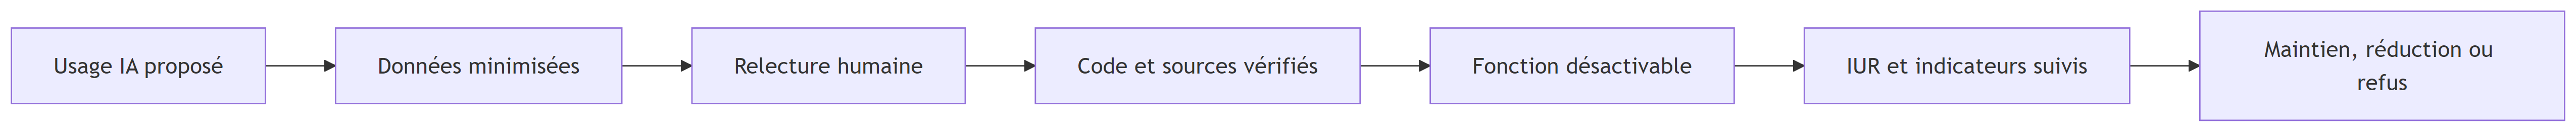
\includegraphics[width=19.13in,height=0.98in]{impact_IA_files/figure-latex/mermaid-figure-2.png}

La règle directrice reste simple : l'IA doit rester un \textbf{assistant
sous contrainte}, et non une couche autonome de décision ou de relation
avec les utilisateurs.

\subsection{Critères d'arrêt, de limitation ou de refus
d'usage}\label{crituxe8res-darruxeat-de-limitation-ou-de-refus-dusage}

Le fait qu'une fonctionnalité IA soit techniquement possible ne suffit
pas à la rendre légitime dans CleanMyMap. À l'inverse, plusieurs
situations doivent conduire à \textbf{ne pas utiliser} l'IA, à en
réduire l'usage ou à désactiver une fonction existante :

\begin{itemize}
\tightlist
\item
  ne pas utiliser l'IA si une \textbf{règle simple} ou un
  \textbf{algorithme déterministe} suffit ;
\item
  ne pas envoyer de \textbf{données personnelles} ou \textbf{sensibles}
  dans les instructions ;
\item
  ne pas utiliser un \textbf{grand modèle} pour une tâche simple ;
\item
  ne pas générer automatiquement un \textbf{contenu} destiné à être
  diffusé sans \textbf{relecture humaine} ;
\item
  ne pas lancer d'\textbf{analyse d'image systématique} si elle
  n'apporte pas un gain réel de qualité, de sécurité ou d'utilité
  terrain ;
\item
  limiter les \textbf{boucles agentiques} ou les \textbf{appels répétés}
  lorsqu'ils augmentent le coût, les dépendances ou le bruit sans
  bénéfice démontré ;
\item
  désactiver les \textbf{fonctionnalités IA peu utilisées} ou
  insuffisamment justifiées par l'usage réel.
\end{itemize}

Autrement dit, l'IA doit être un \textbf{outil d'augmentation ciblée},
pas une \textbf{couche automatique ajoutée partout}.

\subsection{Relecture humaine, documentation et
traçabilité}\label{relecture-humaine-documentation-et-trauxe7abilituxe9}

Pour garantir la rigueur scientifique de cet audit, le présent audit
applique un protocole strict de \textbf{``Human-in-the-loop''} :

\begin{itemize}
\tightlist
\item
  \textbf{Responsable Sobriété} : Une personne identifiée au sein de
  l'équipe (ou un tiers expert) est chargée de valider manuellement
  chaque affirmation technique, chaque calcul d'impact et chaque
  recommandation générée ou suggérée par l'IA.
\item
  \textbf{Droit de Veto} : Le Responsable Sobriété dispose d'un droit de
  veto sur toute fonctionnalité dont le coût écologique n'est pas
  justifié par une utilité terrain immédiate.
\item
  \textbf{Transparence des sources} : Chaque étude citée (GIEC, ADEME,
  Shift Project) doit être accessible et vérifiable.
\item
  \textbf{Droit à la réversibilité} : Toutes les données sont
  exportables pour éviter l'enfermement propriétaire et garantir la
  pérennité de l'audit.
\end{itemize}

Le rapport lui-même entre dans ce protocole : sa rédaction a bénéficié
d'une assistance IA pour structurer, synthétiser et harmoniser les
contenus, mais les chiffres, les sources et les conclusions critiques
doivent rester relus et assumés humainement. Cette méthode réduit le
temps de production documentaire, sans supprimer le risque de coquille,
d'erreur de lien ou de formulation imparfaite ; ces erreurs peuvent être
signalées par courriel à
\href{mailto:contact@cleanmymap.fr}{\nolinkurl{contact@cleanmymap.fr}}.

\subsection{Séparation entre expérimentation, production et décision
sensible}\label{suxe9paration-entre-expuxe9rimentation-production-et-duxe9cision-sensible}

CleanMyMap doit distinguer clairement ce qui relève de l'expérimentation
interne, de la production publiée et de la décision sensible. Un
prototype peut tester un instruction, une structure ou une
fonctionnalité IA, mais rien de sensible ne doit basculer en production
sans relecture, validation et documentation.

Cette séparation évite de confondre un brouillon de travail avec une
décision engageante. Elle protège aussi le rapport lui-même :
l'assistance IA peut aider à préparer, reformuler ou organiser, mais la
version finale publiée doit rester vérifiée humainement, notamment
lorsqu'elle contient des chiffres, des jugements, des arbitrages ou des
engagements de gouvernance.

À titre opérationnel, cette validation n'est pas déclenchée seulement
``en cas de doute'' : elle devient obligatoire dès qu'une sortie de l'IA
touche à un chiffre d'impact, à une décision d'architecture, à la
sécurité, aux données personnelles ou à l'ajout d'une dépendance. Une
proposition est écartée si elle repose sur une source introuvable, sur
une estimation non bornée ou sur un bénéfice terrain difficilement
démontrable.

Des critères simples permettent aussi d'en suivre l'application :

\begin{itemize}
\tightlist
\item
  \textbf{Taux de relecture humaine} : proportion des contenus, calculs
  ou décisions issus de l'IA effectivement revus avant publication.
\item
  \textbf{Taux de rejet ou de correction} : part des propositions IA
  jugées trop coûteuses, trop vagues ou insuffisamment justifiées.
\item
  \textbf{Délai de validation} : temps moyen entre une suggestion IA et
  la décision humaine finale, pour vérifier que la gouvernance reste
  praticable.
\item
  \textbf{Effet mesurable} : nombre de cas où l'IA réduit réellement un
  doublon, un temps de maintenance, un appel réseau ou une complexité
  inutile.
\end{itemize}

Ce protocole ne constitue pas seulement une précaution technique. Il
traduit directement les enseignements DU sur l'autocritique
institutionnalisée, la gouvernance explicite et la capacité d'un projet
environnemental à se fixer lui-même des limites. Dans cette logique, le
\texttt{Responsable\ Sobriété} n'est pas un rôle décoratif : il sert à
arbitrer entre vitesse de production assistée par IA, valeur sociale
réelle et coût numérique cumulé, avec possibilité de bloquer une
fonctionnalité trop coûteuse ou insuffisamment justifiée.

\subsection{Traduction en mesures concrètes pour
CleanMyMap}\label{traduction-en-mesures-concruxe8tes-pour-cleanmymap}

Pour éviter que cette section reste abstraite, chaque risque doit être
relié à une mesure opérationnelle du projet :

\begin{itemize}
\tightlist
\item
  \textbf{Dépendance aux plateformes} : conserver une IA non
  indispensable au coeur du service, des formats d'export simples et des
  fonctions IA désactivables.
\item
  \textbf{Travail invisible} : réserver l'IA aux usages dont la valeur
  est démontrée, suivre ces usages par l'IUR et refuser les usages
  décoratifs.
\item
  \textbf{Perte de maîtrise technique} : imposer revue humaine du code,
  contrôle des dépendances et refus des migrations non relues.
\item
  \textbf{Confidentialité} : limiter les données envoyées, anonymiser
  les logs et interdire les secrets dans les instructions.
\item
  \textbf{Sycophancy, garde-fous fragiles et dépendance émotionnelle} :
  ne pas utiliser l'IA pour des arbitrages sensibles, ni pour
  l'accompagnement émotionnel ; maintenir une supervision humaine et des
  fonctions révocables.
\item
  \textbf{Biais culturels, mésusages et décisions sensibles} : refuser
  toute autorité normative au modèle, maintenir des permissions
  minimales et exclure tout usage décisionnel critique dans CleanMyMap.
\item
  \textbf{Vitesse de déploiement} : appliquer un principe de proportion,
  désactiver les fonctions IA non prouvées et réévaluer en continu
  l'utilité nette.
\end{itemize}

Ces garde-fous ne restent pas théoriques. Ils se prolongent ensuite dans
trois blocs complémentaires du rapport : la \textbf{sobriété
fonctionnelle} et l'\textbf{IUR} en Partie VII pour juger l'utilité
nette, la \textbf{dette numérique} en Partie VIII pour mesurer les coûts
et les effets rebond, et la \textbf{conclusion institutionnelle} en
Partie XII pour fixer la ligne de décision finale.

\section{Bilan social et humanitaire}\label{bilan-social-et-humanitaire}

\subsection{Impacts moins mesurables que le
carbone}\label{impacts-moins-mesurables-que-le-carbone}

Le carbone se mesure en kilowattheures, en kilogrammes de CO₂e et en
litres d'eau. L'impact social et humanitaire de l'IA est, lui, plus
diffus et plus difficile à quantifier. Il touche à l'intégrité
scientifique, à la sécurité logicielle, à la dépendance aux plateformes,
à la santé mentale, au travail invisible, aux contenus sensibles, aux
biais, au pouvoir normatif des modèles et, dans certains contextes, à
des usages militaires ou catastrophiques.

L'impact carbone de l'IA peut être situé par des ordres de grandeur ;
son impact social, lui, se mesure moins facilement, car il touche à la
confiance, à la sécurité, à la production de connaissance, à la
vulnérabilité des personnes et au pouvoir des plateformes.

Le problème n'est donc pas seulement que l'IA consomme : elle peut aussi
produire à grande échelle du code, du texte, des décisions, des images
et des récits qui influencent la société. Cette capacité de production
rend ses effets plus diffus, mais parfois plus profonds que son
empreinte carbone directe.

Cette difficulté de mesure ne doit toutefois pas conduire à une lecture
catastrophiste. Elle impose une vigilance proportionnée et une
évaluation attentive des risques qui ne se voient pas immédiatement mais
qui peuvent peser durablement.

\subsection{Risques humains difficiles à
quantifier}\label{risques-humains-difficiles-uxe0-quantifier}

Parce qu'elle touche aux processus cognitifs, à la production de savoir
et à l'organisation du travail, l'IA transforme la société de manière
structurelle. Elle modifie le rapport collectif à la vérité, à
l'autorité et à l'autonomie. Dans un projet environnemental, cette
transformation peut soit accélérer la transition vers la sobriété, soit
au contraire renforcer des modèles de consommation et de dépendance
technologique insoutenables.

\subsection{Nécessité d'une gouvernance
stricte}\label{nuxe9cessituxe9-dune-gouvernance-stricte}

Cette différence de mesurabilité justifie une gouvernance stricte. Dans
CleanMyMap, l'IA doit rester un assistant, jamais une autorité. Les
sorties doivent être relues. Les fonctionnalités IA doivent être
évaluées par l'IUR. Les données sensibles doivent rester limitées. La
sécurité doit rester prioritaire.

L'IA ne peut donc pas être acceptée comme une force autonome. Elle doit
être encadrée par une gouvernance humaine stricte, transparente et
révocable. Pour CleanMyMap, cela signifie que la technologie reste au
service de la cause environnementale, et non l'inverse. L'IUR (Indice
d'Utilité Réelle) et le protocole de supervision humaine sont les
piliers de cette gouvernance, garantissant que chaque octet consommé et
chaque modèle sollicité serve réellement l'intérêt général.

\section{Apports positifs de l'IA : avancées
scientifiques}\label{apports-positifs-de-lia-avancuxe9es-scientifiques}

L'IA a déjà des intérêts concrets dans plusieurs champs de recherche :
découverte de matériaux, biologie structurale, antibiotiques,
cartographie du cerveau, météorologie, mathématiques, astronomie et
conception de protéines. Elle accélère l'exploration scientifique en
réduisant le temps nécessaire pour tester des hypothèses et en
élargissant l'espace des possibles.

{\def\LTcaptype{none} % do not increment counter
\begin{longtable}[]{@{}
  >{\raggedright\arraybackslash}p{(\linewidth - 4\tabcolsep) * \real{0.3000}}
  >{\raggedleft\arraybackslash}p{(\linewidth - 4\tabcolsep) * \real{0.4000}}
  >{\raggedright\arraybackslash}p{(\linewidth - 4\tabcolsep) * \real{0.3000}}@{}}
\toprule\noalign{}
\begin{minipage}[b]{\linewidth}\raggedright
Corpus étudié
\end{minipage} & \begin{minipage}[b]{\linewidth}\raggedleft
Estimation d'usage IA
\end{minipage} & \begin{minipage}[b]{\linewidth}\raggedright
Prudence d'interprétation
\end{minipage} \\
\midrule\noalign{}
\endhead
\bottomrule\noalign{}
\endlastfoot
PubMed biomédical 2024 & au moins 13,5 \% des abstracts & borne basse,
méthode par vocabulaire \\
Certains sous-corpus biomédicaux & jusqu'à 40 \% & ne vaut pas pour
toute la science \\
Computer science dans certains corpus 2024 & jusqu'à 17,5 \% & selon
Liang et al., corpus arXiv, bioRxiv et Nature \\
Mathématiques / Nature portfolio & jusqu'à 6,3 \% & usage plus faible
dans ce corpus \\
\end{longtable}
}

Sources : (\citeproc{ref-kobak_excess_vocabulary_2025}{Kobak et al.
2025};
\citeproc{ref-liang_increasing_use_llms_scientific_papers_2024}{Liang et
al. 2024})

Ces résultats sont réels, mais ils restent des avancées de recherche.
Ils ne remplacent ni la validation humaine ni les preuves
expérimentales, et ils ne transforment pas encore l'IA en science
autonome. Le détail de ces cas est déplacé en Annexe, afin de garder ici
seulement la synthèse des apports majeurs.

Le point décisif est double : l'IA peut produire des gains réels de
découverte et de calcul, mais ces gains restent concentrés entre les
mains de quelques grands acteurs privés. Cela pose une question de
souveraineté scientifique, d'accès aux infrastructures et de gouvernance
des connaissances.

\section{Lecture par Objectifs de développement durable
(ODD)}\label{lecture-par-objectifs-de-duxe9veloppement-durable-odd}

L'intelligence artificielle transforme profondément la recherche
scientifique moderne. Elle accélère les découvertes, explore des espaces
immenses de possibilités et ouvre de nouveaux champs d'innovation dans
presque toutes les disciplines scientifiques.

L'IA ne constitue pas une ``science autonome'' remplaçant l'humain, mais
un outil de recherche d'une puissance inédite capable d'augmenter
considérablement les capacités scientifiques humaines.

Cependant, cette révolution technologique s'accompagne de nouveaux défis
majeurs : souveraineté scientifique, accès aux infrastructures de
calcul, contrôle des données, dépendance industrielle et gouvernance des
connaissances.

L'avenir dépendra donc autant des progrès techniques de l'IA que des
choix politiques, éthiques et économiques qui encadreront son
développement et son utilisation.

L'IA peut être utile à presque tous les Objectifs de développement
durable, mais elle devient néfaste quand elle augmente les inégalités,
automatise des décisions sensibles, consomme beaucoup de ressources pour
des usages peu utiles, ou renforce la dépendance aux grandes
plateformes. Les 17 ODD constituent le cadre officiel adopté par l'ONU
en 2015; l'ONU estime que l'IA peut aider à accélérer une grande partie
des ODD, mais seulement si elle est encadrée.

Voici le classement le plus pertinent.

{\def\LTcaptype{none} % do not increment counter
\begin{longtable}[]{@{}
  >{\raggedright\arraybackslash}p{(\linewidth - 4\tabcolsep) * \real{0.3333}}
  >{\raggedright\arraybackslash}p{(\linewidth - 4\tabcolsep) * \real{0.3333}}
  >{\raggedright\arraybackslash}p{(\linewidth - 4\tabcolsep) * \real{0.3333}}@{}}
\toprule\noalign{}
\begin{minipage}[b]{\linewidth}\raggedright
ODD
\end{minipage} & \begin{minipage}[b]{\linewidth}\raggedright
IA plutôt utile quand\ldots{}
\end{minipage} & \begin{minipage}[b]{\linewidth}\raggedright
IA plutôt néfaste quand\ldots{}
\end{minipage} \\
\midrule\noalign{}
\endhead
\bottomrule\noalign{}
\endlastfoot
\textbf{ODD 1 --- Pas} & Elle aide à cibler les aides, repérer & Elle
automatise l'exclusion, note les personnes pauvres, refuse des \\
\textbf{de pauvreté} & les besoins, simplifier les & aides sans recours
humain. \\
& démarches sociales. & \\
\textbf{ODD 2 --- Faim} & Elle optimise l'agriculture, prédit les & Elle
favorise une agriculture industrielle dépendante de plateformes, \\
\textbf{``zéro''} & rendements, détecte les maladies & capteurs et
données privées. \\
& des cultures. & \\
\textbf{ODD 3 --- Santé} & Elle aide au diagnostic, au tri & Elle
discrimine des patients, exploite des données de santé ou remplace \\
\textbf{et bien-être} & médical, à la recherche, à la & abusivement le
jugement médical. \\
& prévention. & \\
\textbf{ODD 4 ---} & Elle personnalise l'apprentissage, & Elle favorise
la triche, l'illusion de compétence, la dépendance, ou \\
\textbf{Éducation de} & aide les élèves, traduit, rend le & creuse
l'écart entre élèves équipés et non équipés. \\
\textbf{qualité} & savoir plus accessible. & \\
\textbf{ODD 5 ---} & Elle détecte des discriminations, & Elle reproduit
les biais sexistes des données, discrimine à l'embauche \\
\textbf{Égalité femmes-} & facilite l'accès à l'information et à & ou
amplifie les violences numériques. \\
\textbf{hommes} & certains services. & \\
\textbf{ODD 6 --- Eau} & Elle détecte les fuites, optimise les & Elle
aggrave les conflits locaux d'usage de l'eau autour des data centers. \\
\textbf{propre} & réseaux, surveille la qualité de & \\
& l'eau. & \\
\textbf{ODD 7 ---} & Elle optimise les réseaux & Elle augmente fortement
la demande électrique si les usages explosent \\
\textbf{Énergie propre} & électriques, prédit la production & sans
sobriété. \\
& renouvelable, réduit les pertes. & \\
\textbf{ODD 8 ---} & Elle automatise des tâches & Elle précarise
certains métiers, intensifie le travail, invisibilise les \\
\textbf{Travail décent} & pénibles, aide les petites structures, &
travailleurs de l'annotation et de la modération. \\
& augmente les capacités de & \\
& production. & \\
\textbf{ODD 9 ---} & Elle accélère la recherche, la & Elle concentre
l'innovation chez quelques acteurs qui contrôlent \\
\textbf{Industrie,} & maintenance, la logistique, la & modèles, cloud et
puces. \\
\textbf{innovation,} & conception technique. & \\
\textbf{infrastructures} & & \\
\textbf{ODD 10 ---} & Elle peut rendre des outils & Elle creuse l'écart
entre ceux qui ont données, calcul, argent et \\
\textbf{Inégalités} & puissants accessibles à des petites & compétences,
et ceux qui n'y ont pas accès. \\
\textbf{réduites} & équipes ou pays moins dotés. & \\
\textbf{ODD 11 --- Villes} & Elle optimise transports, énergie, & Elle
devient un outil de surveillance urbaine ou de contrôle social. \\
\textbf{durables} & déchets, voirie, cartographie des & \\
& besoins. & \\
\end{longtable}
}

{\def\LTcaptype{none} % do not increment counter
\begin{longtable}[]{@{}
  >{\raggedright\arraybackslash}p{(\linewidth - 4\tabcolsep) * \real{0.3333}}
  >{\raggedright\arraybackslash}p{(\linewidth - 4\tabcolsep) * \real{0.3333}}
  >{\raggedright\arraybackslash}p{(\linewidth - 4\tabcolsep) * \real{0.3333}}@{}}
\toprule\noalign{}
\begin{minipage}[b]{\linewidth}\raggedright
ODD
\end{minipage} & \begin{minipage}[b]{\linewidth}\raggedright
IA plutôt utile quand\ldots{}
\end{minipage} & \begin{minipage}[b]{\linewidth}\raggedright
IA plutôt néfaste quand\ldots{}
\end{minipage} \\
\midrule\noalign{}
\endhead
\bottomrule\noalign{}
\endlastfoot
\textbf{ODD 12 ---} & Elle aide à réduire le gaspillage, & Elle stimule
la surproduction de contenus, la publicité ciblée, \\
\textbf{Consommation} & prévoir les stocks, analyser les &
l'obsolescence et la consommation numérique inutile. \\
\textbf{responsable} & cycles de vie. & \\
\textbf{ODD 13 ---} & Elle améliore les prévisions, & Elle consomme
beaucoup d'énergie pour des usages à faible utilité \\
\textbf{Climat} & optimise l'énergie, modélise les & sociale. L'ITU
(\citeproc{ref-itu_artificial_intelligence}{ITU, n.d.}) indique que l'IA
peut aider les ODD, mais souligne \\
& risques, aide à réduire les & aussi la nécessité de gouvernance pour
éviter les effets négatifs. \\
& émissions. & \\
\textbf{ODD 14 --- Vie} & Elle surveille pollution, pêche & Elle
contribue indirectement à la pression énergétique, minière et \\
\textbf{aquatique} & illégale, qualité de l'eau, & matérielle du
numérique. \\
& biodiversité marine. & \\
\textbf{ODD 15 --- Vie} & Elle aide à suivre la déforestation, & Elle
dépend de matériel numérique dont l'extraction peut abîmer des \\
\textbf{terrestre} & les espèces, les incendies, les sols. & milieux
naturels. \\
\textbf{ODD 16 --- Paix,} & Elle aide à analyser des données & Elle
produit deepfakes, surveillance, manipulation politique, décisions \\
\textbf{justice,} & publiques, détecter corruption ou & opaques.
L'ONU{[}45{]}et l'ITU{[}46{]} {[}47{]}alertent notamment sur les \\
\textbf{institutions} & désinformation. & risques de deepfakes et de
désinformation. \\
\textbf{ODD 17 ---} & Elle facilite la coopération, la & Elle renforce
la dépendance aux grandes entreprises privées et aux \\
\textbf{Partenariats} & traduction, le partage de données & pays qui
contrôlent l'infrastructure IA. \\
& et la coordination. & \\
\end{longtable}
}

L'IA est particulièrement utile pour les ODD où l'analyse de données, la
prédiction, l'optimisation ou l'accessibilité jouent un rôle important :
santé, éducation, énergie, climat, villes durables, agriculture,
biodiversité et gestion de l'eau. Elle peut aider à mieux mesurer,
prévoir et coordonner l'action humaine. En revanche, elle devient
problématique lorsqu'elle touche aux droits humains, à l'accès aux
services essentiels, à la surveillance, au travail ou aux inégalités;
les ODD les plus sensibles sont donc ceux liés à la pauvreté, au travail
décent, aux inégalités, à la justice et aux institutions.

Dans le cas de CleanMyMap, le projet d'engagement bénévole peut être
relié positivement à :

{\def\LTcaptype{none} % do not increment counter
\begin{longtable}[]{@{}
  >{\raggedright\arraybackslash}p{(\linewidth - 6\tabcolsep) * \real{0.2500}}
  >{\raggedright\arraybackslash}p{(\linewidth - 6\tabcolsep) * \real{0.2500}}
  >{\raggedright\arraybackslash}p{(\linewidth - 6\tabcolsep) * \real{0.2500}}
  >{\raggedright\arraybackslash}p{(\linewidth - 6\tabcolsep) * \real{0.2500}}@{}}
\toprule\noalign{}
\begin{minipage}[b]{\linewidth}\raggedright
ODD
\end{minipage} & \begin{minipage}[b]{\linewidth}\raggedright
\end{minipage} & \begin{minipage}[b]{\linewidth}\raggedright
\end{minipage} & \begin{minipage}[b]{\linewidth}\raggedright
Lien avec CleanMyMap
\end{minipage} \\
\midrule\noalign{}
\endhead
\bottomrule\noalign{}
\endlastfoot
\textbf{ODD} & \textbf{11} & \textbf{--- Villes durables} & actions
locales de propreté, amélioration de l'espace public \\
\textbf{ODD} & \textbf{12} & \textbf{--- Consommation responsable} &
sensibilisation aux déchets, mégots, pollution urbaine \\
\textbf{ODD} & \textbf{13} & \textbf{--- Climat} & réflexion sur
l'impact numérique et sobriété des usages \\
\textbf{ODD} & \textbf{14} & \textbf{--- Vie aquatique} & réduction des
mégots pouvant contaminer l'eau \\
\textbf{ODD} & \textbf{15} & \textbf{--- Vie terrestre} & retrait de
déchets de l'environnement urbain \\
\textbf{ODD} & \textbf{17} & \textbf{--- Partenariats} & mobilisation de
bénévoles, associations, citoyens \\
\end{longtable}
}

Mais tu peux aussi reconnaître les risques :

{\def\LTcaptype{none} % do not increment counter
\begin{longtable}[]{@{}
  >{\raggedright\arraybackslash}p{(\linewidth - 2\tabcolsep) * \real{0.5000}}
  >{\raggedright\arraybackslash}p{(\linewidth - 2\tabcolsep) * \real{0.5000}}@{}}
\toprule\noalign{}
\begin{minipage}[b]{\linewidth}\raggedright
Risque IA
\end{minipage} & \begin{minipage}[b]{\linewidth}\raggedright
ODD concerné
\end{minipage} \\
\midrule\noalign{}
\endhead
\bottomrule\noalign{}
\endlastfoot
Dépendance à Codex, OpenAI, Claude, Vercel, Supabase, Stripe, etc. & ODD
9, 10, 17 \\
Consommation électrique et eau des data centers & ODD 6, 7, 13 \\
Travail invisible de l'annotation/modération & ODD 8, 10 \\
Inégalités d'accès aux outils IA & ODD 4, 10 \\
Données utilisateurs et surveillance potentielle & ODD 16 \\
Production excessive de code, churn, complexité technique & ODD 12,
13 \\
\end{longtable}
}

\section{Gouvernance humaine et pilotage du
projet}\label{gouvernance-humaine-et-pilotage-du-projet}

Dans le cas de CleanMyMap, l'IA n'est pertinente que si elle renforce la
capacité à agir sur la propreté urbaine sans dégrader la rigueur du
produit ni la responsabilité environnementale.

\subsection{Apports concrets de l'IA pour le développement du
site}\label{apports-concrets-de-lia-pour-le-duxe9veloppement-du-site}

\begin{itemize}
\item
  Rapidité d'exécution : l'IA accélère les tâches de cadrage, de
  rédaction technique, de structuration et de prototypage.
\item
  Productivité technique : génération de premiers jets de code, aide au
  refactor, proposition de tests, accélération du débogage.
\item
  Idéation et structuration : transformation de notes brutes en plans
  exploitables, décomposition en lots, priorisation des dépendances.
\item
  Accessibilité technique : réduction du seuil d'entrée sur des sujets
  complexes (architecture, tests, instrumentation, documentation).
\item
  Support éditorial : reformulation de contenus, clarté des messages,
  harmonisation de la tonalité entre pages.
\item
  Appui opérationnel : accélération de la production de docs,
  checklists, runbooks et synthèses pour coordination équipe/jury.
\end{itemize}

Appliqués à CleanMyMap, ces apports sont pertinents lorsque l'IA sert
des objectifs concrets : meilleure lisibilité des parcours, meilleure
qualité des livrables, meilleure capacité de pilotage et réduction du
temps perdu sur des tâches répétitives.

\subsection{Limites, risques et effets
pervers}\label{limites-risques-et-effets-pervers}

\begin{itemize}
\item
  Superficialité : l'IA peut fournir des réponses plausibles mais
  fragiles, surtout sans vérification contextuelle du repo.
\item
  Hallucinations et erreurs : références techniques, juridiques ou
  factuelles potentiellement inexactes.
\item
  Dette technique : génération rapide de code hétérogène, couplage
  excessif, conventions incohérentes.
\item
  Standardisation excessive : interfaces et formulations trop
  génériques, perte d'adéquation aux usages réels des utilisateurs.
\item
  Baisse d'esprit critique : risque de valider trop vite des
  propositions non testées.
\item
  Risques sécurité/confidentialité : exposition de données sensibles si
  les instructions incluent des informations personnelles ou internes
  inutiles.
\item
  Mauvais arbitrages architecture : optimisation locale rapide au
  détriment de la maintenabilité globale.
\item
  Impact environnemental indirect : même si l'impact unitaire peut
  paraître modeste, le volume cumulé de requêtes, d'itérations et
  d'agents peut devenir significatif.
\item
  \textbf{Effet Rebond (Paradoxe de Jevons)} : La facilité de
  développement accrue par l'IA peut inciter à créer des fonctionnalités
  superflues ( \emph{dérive fonctionnelle} ), annulant ainsi les gains
  de sobriété réalisés sur le code lui-même.
\item
  \textbf{Inflation de code (gonflement induit par l'IA)} : L'IA a
  tendance à générer plus de code que nécessaire si elle n'est pas
  contrainte par une exigence de minimalisme extrême.
\end{itemize}

\subsection{Compromis à arbitrer}\label{compromis-uxe0-arbitrer}

Compromis 1 - Vitesse vs fiabilité : l'IA augmente la vitesse de
production, mais cette vitesse est utile uniquement si les sorties sont
vérifiées (tests, revue humaine, cohérence produit).

Compromis 2 - Productivité vs qualité architecture : un gain de court
terme peut fabriquer de la dette long terme si les décisions ne sont pas
tracées et rationalisées.

Compromis 3 - Assistance vs dépendance : l'IA doit rester un
accélérateur. Elle ne remplace ni la capacité d'analyse de l'équipe ni
la prise de décision.

Compromis 4 - Efficacité numérique vs cohérence écologique : utiliser
intensivement l'IA pour un projet environnemental peut créer une tension
de crédibilité si la sobriété numérique n'est pas intégrée (instructions
mieux ciblés, moins d'itérations inutiles, priorisation des tâches à
forte valeur).

\section{Arbitrage final}\label{arbitrage-final}

En synthèse, l'IA est utile pour CleanMyMap lorsqu'elle sert une logique
d'amélioration mesurable : mieux structurer, mieux coder, mieux tester
et mieux communiquer. Elle devient contre-productive dès qu'elle
remplace le jugement critique, dégrade la cohérence technique ou
affaiblit la responsabilité environnementale du projet. La bonne posture
reste pragmatique : IA pour accélérer, humain pour arbitrer, vérifier et
assumer la décision finale.

Une fois cette position clarifiée, il faut encore la traduire en
priorités concrètes sur le produit et dans l'organisation.

\textbf{Coût énergétique : pourquoi ne pas considérer l'IA comme
incompatible avec le projet?} Le rapport ne nie pas le coût énergétique
de l'IA.

\begin{itemize}
\item
  \textbf{Mode dégradé} : Fonctionnement minimal permettant de maintenir
  les usages essentiels lorsqu'un service externe est indisponible.
\item
  \textbf{WUE (Water Usage Effectiveness)} : Indicateur mesurant
  l'efficacité de l'utilisation de l'eau dans un data center (Litre
  d'eau par kWh consommé)
\end{itemize}

L'IA est souvent présentée comme un accélérateur potentiel des Objectifs
de développement durable (ODD), mais cette promesse n'est valable que
sous conditions. Le même outil peut aider un objectif dans un contexte
et l'aggraver dans un autre.

Pour CleanMyMap, les ODD les plus directement concernés sont les
suivants :

{\def\LTcaptype{none} % do not increment counter
\begin{longtable}[]{@{}
  >{\raggedright\arraybackslash}p{(\linewidth - 4\tabcolsep) * \real{0.3333}}
  >{\raggedright\arraybackslash}p{(\linewidth - 4\tabcolsep) * \real{0.3333}}
  >{\raggedright\arraybackslash}p{(\linewidth - 4\tabcolsep) * \real{0.3333}}@{}}
\toprule\noalign{}
\begin{minipage}[b]{\linewidth}\raggedright
ODD
\end{minipage} & \begin{minipage}[b]{\linewidth}\raggedright
Contribution potentielle de CleanMyMap
\end{minipage} & \begin{minipage}[b]{\linewidth}\raggedright
Risque si l'IA ou le numérique sont mal cadrés
\end{minipage} \\
\midrule\noalign{}
\endhead
\bottomrule\noalign{}
\endlastfoot
\textbf{ODD 11 --- Villes durables} & meilleure localisation des
déchets, coordination locale, cartographie d'usage & outil de
surveillance ou surcouche numérique peu utilisée \\
\textbf{ODD 12 --- Consommation responsable} & meilleure traçabilité,
réduction des doublons, sensibilisation aux déchets & inflation de
contenus, stockage excessif, complexité inutile \\
\textbf{ODD 13 --- Climat} & pilotage plus sobre, meilleure coordination
d'actions utiles & hausse de la consommation électrique pour des usages
peu utiles \\
\textbf{ODD 14 et 15 --- Vie aquatique et terrestre} & diminution locale
de déchets abandonnés, documentation des zones touchées & coût matériel
et énergétique du numérique mal maîtrisé \\
\textbf{ODD 17 --- Partenariats} & meilleure coopération entre
bénévoles, associations, collectifs et collectivités & dépendance accrue
à quelques plateformes privées \\
\end{longtable}
}

Cette lecture par ODD ne doit pas être utilisée comme un label
automatique. Elle sert au contraire à rappeler que la cohérence d'un
projet écologique dépend autant de sa gouvernance, de sa sobriété et de
sa réversibilité que de sa finalité affichée.

Pour conserver la granularité de l'ancienne version, il faut expliciter
davantage cette lecture :

{\def\LTcaptype{none} % do not increment counter
\begin{longtable}[]{@{}
  >{\raggedright\arraybackslash}p{(\linewidth - 4\tabcolsep) * \real{0.3333}}
  >{\raggedright\arraybackslash}p{(\linewidth - 4\tabcolsep) * \real{0.3333}}
  >{\raggedright\arraybackslash}p{(\linewidth - 4\tabcolsep) * \real{0.3333}}@{}}
\toprule\noalign{}
\begin{minipage}[b]{\linewidth}\raggedright
ODD
\end{minipage} & \begin{minipage}[b]{\linewidth}\raggedright
IA plutôt utile quand\ldots{}
\end{minipage} & \begin{minipage}[b]{\linewidth}\raggedright
IA plutôt néfaste quand\ldots{}
\end{minipage} \\
\midrule\noalign{}
\endhead
\bottomrule\noalign{}
\endlastfoot
\textbf{ODD 1 --- Pas de pauvreté} & elle aide à cibler les aides,
repérer les besoins, simplifier les démarches sociales & elle automatise
l'exclusion, note les personnes pauvres, refuse des aides sans recours
humain \\
\textbf{ODD 2 --- Faim ``zéro''} & elle optimise l'agriculture, prédit
les rendements, détecte les maladies des cultures & elle favorise une
agriculture industrielle dépendante de plateformes, capteurs et données
privées \\
\textbf{ODD 3 --- Santé et bien-être} & elle aide au diagnostic, au tri
médical, à la recherche, à la prévention & elle discrimine des patients,
exploite des données de santé ou remplace abusivement le jugement
médical \\
\textbf{ODD 4 --- Éducation de qualité} & elle personnalise
l'apprentissage, aide les élèves, traduit, rend le savoir plus
accessible & elle favorise la triche, l'illusion de compétence, la
dépendance, ou creuse l'écart entre élèves équipés et non équipés \\
\textbf{ODD 5 --- Égalité femmes-hommes} & elle détecte des
discriminations, facilite l'accès à l'information et à certains services
& elle reproduit les biais sexistes des données, discrimine à l'embauche
ou amplifie les violences numériques \\
\textbf{ODD 6 --- Eau propre} & elle détecte les fuites, optimise les
réseaux, surveille la qualité de l'eau & elle aggrave les conflits
locaux d'usage de l'eau autour des data centers \\
\textbf{ODD 7 --- Énergie propre} & elle optimise les réseaux
électriques, prédit la production renouvelable, réduit les pertes & elle
augmente fortement la demande électrique si les usages explosent sans
sobriété \\
\textbf{ODD 8 --- Travail décent} & elle automatise des tâches pénibles,
aide les petites structures, augmente les capacités de production & elle
précarise certains métiers, intensifie le travail, invisibilise les
travailleurs de l'annotation et de la modération \\
\textbf{ODD 9 --- Industrie, innovation, infrastructures} & elle
accélère la recherche, la maintenance, la logistique, la conception
technique & elle concentre l'innovation chez quelques acteurs qui
contrôlent modèles, cloud et puces \\
\textbf{ODD 10 --- Inégalités réduites} & elle peut rendre des outils
puissants accessibles à des petites équipes ou pays moins dotés & elle
creuse l'écart entre ceux qui ont données, calcul, argent et
compétences, et ceux qui n'y ont pas accès \\
\textbf{ODD 11 --- Villes durables} & elle optimise transports, énergie,
déchets, voirie, cartographie des besoins & elle devient un outil de
surveillance urbaine ou de contrôle social \\
\textbf{ODD 12 --- Consommation responsable} & elle aide à réduire le
gaspillage, prévoir les stocks, analyser les cycles de vie & elle
stimule la surproduction de contenus, la publicité ciblée,
l'obsolescence et la consommation numérique inutile \\
\textbf{ODD 13 --- Climat} & elle améliore les prévisions, optimise
l'énergie, modélise les risques, aide à réduire les émissions & elle
consomme beaucoup d'énergie pour des usages à faible utilité sociale \\
\textbf{ODD 14 --- Vie aquatique} & elle surveille pollution, pêche
illégale, qualité de l'eau, biodiversité marine & elle contribue
indirectement à la pression énergétique, minière et matérielle du
numérique \\
\textbf{ODD 15 --- Vie terrestre} & elle aide à suivre la déforestation,
les espèces, les incendies, les sols & elle dépend de matériel numérique
dont l'extraction peut abîmer des milieux naturels \\
\textbf{ODD 16 --- Paix, justice, institutions} & elle aide à analyser
des données publiques, détecter corruption ou désinformation & elle
produit deepfakes, surveillance, manipulation politique, décisions
opaques \\
\textbf{ODD 17 --- Partenariats} & elle facilite la coopération, la
traduction, le partage de données et la coordination & elle renforce la
dépendance aux grandes entreprises privées et aux pays qui contrôlent
l'infrastructure IA \\
\end{longtable}
}

Pour CleanMyMap, cette grille peut être traduite plus concrètement :

{\def\LTcaptype{none} % do not increment counter
\begin{longtable}[]{@{}
  >{\raggedright\arraybackslash}p{(\linewidth - 2\tabcolsep) * \real{0.5000}}
  >{\raggedright\arraybackslash}p{(\linewidth - 2\tabcolsep) * \real{0.5000}}@{}}
\toprule\noalign{}
\begin{minipage}[b]{\linewidth}\raggedright
ODD
\end{minipage} & \begin{minipage}[b]{\linewidth}\raggedright
Lien positif probable avec le projet
\end{minipage} \\
\midrule\noalign{}
\endhead
\bottomrule\noalign{}
\endlastfoot
\textbf{ODD 11 --- Villes durables} & actions locales de propreté,
amélioration de l'espace public \\
\textbf{ODD 12 --- Consommation responsable} & sensibilisation aux
déchets, mégots, pollution urbaine \\
\textbf{ODD 13 --- Climat} & réflexion sur l'impact numérique et
sobriété des usages \\
\textbf{ODD 14 --- Vie aquatique} & réduction des mégots pouvant
contaminer l'eau \\
\textbf{ODD 15 --- Vie terrestre} & retrait de déchets de
l'environnement urbain \\
\textbf{ODD 17 --- Partenariats} & mobilisation de bénévoles,
associations, citoyens \\
\end{longtable}
}

Et les risques doivent rester formulés eux aussi :

{\def\LTcaptype{none} % do not increment counter
\begin{longtable}[]{@{}
  >{\raggedright\arraybackslash}p{(\linewidth - 2\tabcolsep) * \real{0.5000}}
  >{\raggedright\arraybackslash}p{(\linewidth - 2\tabcolsep) * \real{0.5000}}@{}}
\toprule\noalign{}
\begin{minipage}[b]{\linewidth}\raggedright
Risque IA ou numérique
\end{minipage} & \begin{minipage}[b]{\linewidth}\raggedright
ODD concerné
\end{minipage} \\
\midrule\noalign{}
\endhead
\bottomrule\noalign{}
\endlastfoot
dépendance à Codex, OpenAI, Claude, Vercel, Supabase, Stripe, etc. & ODD
9, 10, 17 \\
consommation électrique et eau des data centers & ODD 6, 7, 13 \\
travail invisible de l'annotation/modération & ODD 8, 10 \\
inégalités d'accès aux outils IA & ODD 4, 10 \\
données utilisateurs et surveillance potentielle & ODD 16 \\
production excessive de code, churn, complexité technique & ODD 12,
13 \\
\end{longtable}
}

Cette version plus longue est utile parce qu'elle évite de réduire la
référence aux ODD à un simple habillage institutionnel. Elle rappelle
qu'un même projet peut contribuer à certains objectifs tout en
fragilisant d'autres dimensions s'il perd sa discipline de sobriété.

\textbf{Apports concrets de l'IA pour le développement du site}

\begin{itemize}
\tightlist
\item
  rapidité d'exécution : accélération du cadrage, de la rédaction
  technique, de la structuration et du prototypage ;
\item
  productivité technique : génération de premiers jets de code, aide au
  refactor, proposition de tests, accélération du débogage ;
\item
  idéation et structuration : transformation de notes brutes en plans
  exploitables, décomposition en lots, priorisation des dépendances ;
\item
  accessibilité technique : réduction du seuil d'entrée sur des sujets
  complexes ;
\item
  support éditorial : reformulation de contenus, clarté des messages,
  harmonisation de la tonalité entre pages ;
\item
  appui opérationnel : accélération de la production de docs,
  checklists, runbooks et synthèses.
\end{itemize}

Appliqués à CleanMyMap, ces apports ne sont pertinents que lorsqu'ils
servent des objectifs concrets : meilleure lisibilité des parcours,
meilleure qualité des livrables, meilleure capacité de pilotage et
réduction du temps perdu sur des tâches répétitives. L'intérêt de l'IA
ne se mesure donc pas ici au nombre de sorties produites, mais à sa
capacité à renforcer un système sociotechnique déjà compréhensible,
gouvernable et utile au terrain.

\textbf{Limites, risques et effets pervers}

\begin{itemize}
\tightlist
\item
  superficialité : réponses plausibles mais fragiles sans vérification
  contextuelle du dépôt ;
\item
  hallucinations et erreurs : références techniques, juridiques ou
  factuelles potentiellement inexactes ;
\item
  dette technique : génération rapide de code hétérogène, couplage
  excessif, conventions incohérentes ;
\item
  standardisation excessive : interfaces et formulations trop génériques
  ;
\item
  baisse d'esprit critique : validation trop rapide de propositions non
  testées ;
\item
  risques sécurité/confidentialité : exposition de données sensibles si
  les instructions incluent des informations inutiles ;
\item
  mauvais arbitrages architecture : optimisation locale rapide au
  détriment de la maintenabilité globale ;
\item
  impact environnemental indirect : accumulation de requêtes,
  d'itérations et d'agents ;
\item
  effet rebond : facilité de développement pouvant inciter à créer des
  fonctionnalités superflues ;
\item
  inflation de code : tendance des modèles à générer plus de code que
  nécessaire.
\end{itemize}

Ces limites sont importantes parce qu'elles déplacent la question de
l'IA depuis la performance brute vers la qualité de gouvernance. Un
projet environnemental peut perdre sa cohérence si l'IA accroît plus
vite la dépendance, le volume de code ou la dette d'architecture qu'elle
n'améliore réellement le service rendu.

\textbf{Compromis à arbitrer}

\begin{itemize}
\tightlist
\item
  vitesse vs fiabilité ;
\item
  productivité vs qualité d'architecture ;
\item
  assistance vs dépendance ;
\item
  efficacité numérique vs cohérence écologique.
\end{itemize}

La synthèse responsable à conserver est la suivante : l'IA n'est ni à
rejeter par principe, ni à adopter aveuglément. Elle n'est justifiée que
si elle augmente clairement l'utilité nette du projet, puis elle doit
être limitée dès qu'elle ajoute surtout du volume, de la dépendance ou
du bruit numérique.

\subsection{Conditions d'un usage responsable et pertinent de
l'IA}\label{conditions-dun-usage-responsable-et-pertinent-de-lia}

L'usage de l'IA ne devient défendable qu'à l'intérieur d'un cadre
explicite. Le PDF le plus récent insistait sur un point utile à
conserver dans le corps du rapport : une IA acceptable n'est pas une IA
``performante'' en général, mais une IA \textbf{sous surveillance},
c'est-à-dire bornée par des règles de validation, de traçabilité et de
sobriété.

\begin{itemize}
\tightlist
\item
  gouvernance claire : définir ce que l'IA peut proposer et ce que seul
  l'humain peut valider ;
\item
  vérification systématique : tests, revue de code et vérification
  factuelle pour les contenus ;
\item
  hygiène des données : minimisation, anonymisation et exclusion des
  informations sensibles ;
\item
  traçabilité des décisions : distinguer suggestion IA, décision produit
  et validation finale ;
\item
  cadre de qualité : conventions de code, standards UX, schéma
  d'événements et check-list de sortie ;
\item
  cohérence environnementale : réserver l'IA aux usages à forte valeur
  et éviter les itérations peu utiles ;
\item
  transparence : expliciter les zones assistées par IA et les contrôles
  humains associés.
\end{itemize}

Autrement dit, l'IA n'est pas ici un supplément de modernité. Elle est
un levier sous contrainte, dont l'usage doit rester proportionné,
mesurable, désactivable et continuellement réévaluable à partir de
l'utilité réelle du projet.

\section{Synthèse : dépendance, pouvoir et vulnérabilité
systémique}\label{synthuxe8se-duxe9pendance-pouvoir-et-vulnuxe9rabilituxe9-systuxe9mique}

\subsection{L'IA comme infrastructure de
dépendance}\label{lia-comme-infrastructure-de-duxe9pendance}

La Partie IV montre que l'IA n'est pas seulement une couche logicielle
ajoutée au projet. Elle fonctionne aussi comme une infrastructure de
dépendance, car elle repose sur des clouds, des modèles propriétaires,
des GPU, des API et des fournisseurs dont CleanMyMap ne maîtrise ni la
disponibilité, ni les prix, ni les règles d'accès. Même lorsqu'elle
accélère le développement, cette architecture introduit des dépendances
structurelles qui dépassent le simple confort d'usage.

\subsection{Risque de perte d'autonomie technique et
politique}\label{risque-de-perte-dautonomie-technique-et-politique}

Le principal risque associé à cette concentration est la perte
d'autonomie. Sur le plan technique, le projet peut devenir difficile à
faire évoluer sans un fournisseur unique, un service externe ou une pile
propriétaire. Sur le plan politique, il peut aussi devenir tributaire de
choix industriels, réglementaires ou géopolitiques qu'il ne contrôle
pas. Pour CleanMyMap, l'enjeu n'est donc pas d'éviter toute dépendance,
mais de conserver une souveraineté fonctionnelle réelle : comprendre,
documenter, réduire et remplacer les briques critiques avant qu'elles ne
deviennent des points de blocage.

\subsection{Nécessité d'une gouvernance publique et
collective}\label{nuxe9cessituxe9-dune-gouvernance-publique-et-collective}

À cette échelle, la réponse ne peut pas reposer uniquement sur des
arbitrages individuels de développeur. Les dépendances numériques, les
effets de concentration et les risques systémiques appellent une
gouvernance publique et collective : règles européennes de protection
des données, exigences de transparence, documentation des modèles,
possibilité d'audit, réduction du verrouillage et soutien à des
alternatives ouvertes ou mutualisées. Pour CleanMyMap, cela signifie que
l'usage de l'IA doit rester compatible avec des standards plus larges
que les seules contraintes du projet : traçabilité, réversibilité,
sobriété et responsabilité partagée.

\newpage{}

\chapter{Partie V --- Risques techniques, sécurité et contrôle des
systèmes
d'IA}\label{partie-v-risques-techniques-securite-et-controle-des-systemes-dia}

Cette partie descend d'un niveau : après les dépendances systémiques,
elle analyse les risques concrets liés à l'usage technique des modèles,
à la génération de code, à la cybersécurité, aux données et aux limites
des garde-fous.

\section{Confidentialité, données et responsabilité
juridique}\label{confidentialituxe9-donnuxe9es-et-responsabilituxe9-juridique}

\subsection{Données sensibles dans les instructions et les fichiers
transmis}\label{donnuxe9es-sensibles-dans-les-instructions-et-les-fichiers-transmis}

Le quatrième risque est celui de la \textbf{confidentialité}. Les
instructions envoyés à une IA peuvent contenir beaucoup plus
d'informations sensibles qu'il n'y paraît : architecture du projet,
extraits de code, erreurs serveur, logs, schémas de base de données,
données métier, noms d'utilisateurs, informations personnelles, clés
API, jetons, secrets ou variables d'environnement. Un instruction doit
donc être traité comme un canal de transmission de données, et non comme
une simple zone de texte sans conséquence.

Cette vigilance est particulièrement importante dans un projet comme
CleanMyMap. Le site peut manipuler des signalements localisés, des
photos, des comptes utilisateurs, des rôles, des exports, des données
associatives ou des informations institutionnelles. Même lorsqu'un
instruction ne contient pas directement une donnée personnelle évidente,
il peut contenir des éléments permettant une réidentification indirecte
: adresse, coordonnées, identifiant technique, historique d'action,
capture d'écran ou extrait de base de données. L'usage de l'IA doit donc
respecter un principe de minimisation : ne transmettre que ce qui est
strictement nécessaire à la tâche.

Sur le plan opérationnel, certaines informations ne doivent jamais être
envoyées à un outil IA : \textbf{clés API}, \textbf{secrets},
\textbf{jetons}, \textbf{mots de passe}, \textbf{variables
d'environnement}, URLs privées, chaînes de connexion, dumps de base de
données ou données personnelles non anonymisées. La CNIL rappelle
également que la sécurité des clés d'accès aux API ne doit pas être
négligée et qu'elles doivent être protégées comme des secrets
techniques, par exemple via des mécanismes de stockage sécurisé.

Les logs, erreurs et extraits de base de données doivent être
\textbf{anonymisés} avant tout partage avec une IA. Cela signifie
retirer ou remplacer les noms, emails, identifiants, adresses,
coordonnées GPS précises, numéros de téléphone, jetons, IDs de session
et toute information permettant de retrouver une personne ou un compte.
Dans le doute, il faut réduire le contexte envoyé plutôt que transmettre
un extrait complet. Un modèle peut aider à corriger une erreur sans
recevoir tout l'historique applicatif ni les données réelles des
utilisateurs (\citeproc{ref-nist_artificial_intelligence_3}{NIST,
n.d.-b}; \citeproc{ref-cnil_s_curit}{CNIL, n.d.-e}).

Le même principe vaut pour le code produit. Tout \textbf{code généré par
IA} doit être relu, testé et discuté avant intégration. Les
\textbf{dépendances ajoutées} doivent être vérifiées, car une
bibliothèque proposée automatiquement peut accroître inutilement le
bundle, introduire une faille, exposer une donnée ou créer une dette de
maintenance. L'OWASP classe d'ailleurs les risques liés à la chaîne
d'approvisionnement et aux dépendances parmi les vulnérabilités
importantes des applications utilisant des modèles de langage.

\subsection{RGPD, consentement et minimisation des
données}\label{rgpd-consentement-et-minimisation-des-donnuxe9es}

Le RGPD impose plusieurs principes directement applicables à l'usage de
l'IA dans un contexte européen : finalité limitée, minimisation des
données, transparence, sécurité, durée de conservation proportionnée,
droits des personnes et responsabilité du responsable de traitement. Ces
principes s'appliquent dès qu'un système traite des \textbf{données à
caractère personnel}, c'est-à-dire toute information permettant
d'identifier directement ou indirectement une personne.

Dans CleanMyMap, les données sensibles ne se limitent pas aux noms,
emails ou comptes utilisateurs. Des photos géolocalisées peuvent aussi
devenir des données personnelles si elles montrent une personne, une
plaque d'immatriculation, un visage, un commerce identifiable, un
domicile, une adresse précise ou un élément permettant de relier un
signalement à un individu. Une simple photo de déchet peut donc changer
de statut selon son contenu, son contexte et les métadonnées associées.

L'usage d'API d'IA pour analyser automatiquement des images, reformuler
des signalements ou classer des contenus peut constituer un traitement
de données personnelles si les éléments transmis permettent d'identifier
une personne ou un lieu précis associé à une personne. Ce traitement
doit alors être justifié par une finalité claire, expliqué aux
utilisateurs et limité aux données strictement nécessaires. Le fait
qu'un traitement soit techniquement possible ne suffit pas à le rendre
conforme.

La minimisation doit être appliquée dès la conception. CleanMyMap doit
éviter d'envoyer à une API externe des images complètes si une version
compressée, floutée, recadrée ou anonymisée suffit. Les visages, plaques
d'immatriculation, adresses précises, coordonnées GPS trop fines et
métadonnées inutiles doivent être supprimés ou masqués lorsque leur
conservation n'est pas nécessaire. De même, les instructions envoyés à
un modèle ne doivent pas contenir de noms, emails, identifiants, logs
personnels ou données de compte si la tâche peut être réalisée avec un
exemple générique.

Le consentement ne doit pas être traité comme une simple case à cocher.
Lorsque l'utilisateur transmet une photo ou un signalement, il doit
comprendre quelles données sont collectées, pourquoi elles le sont,
combien de temps elles sont conservées, qui peut y accéder, et si elles
peuvent être transmises à un service externe d'IA. Si une analyse
automatique d'image ou de texte est utilisée, cette information doit
apparaître clairement dans la politique de confidentialité et, si
nécessaire, dans l'interface de dépôt.

Le projet doit aussi distinguer les traitements internes et externes.
Une classification simple réalisée localement ou par une règle
déterministe ne pose pas les mêmes enjeux qu'un envoi vers une API d'IA
tierce. Dans le second cas, il faut vérifier le fournisseur, la région
de traitement si elle est disponible, les conditions de conservation des
données, la possibilité d'exclusion de l'entraînement, les
sous-traitants, les garanties contractuelles et la conformité avec les
règles européennes de protection des données.

Si un traitement IA est susceptible d'engendrer un risque élevé pour les
droits et libertés des personnes, une \textbf{AIPD} doit être envisagée
avant la mise en œuvre. C'est particulièrement important si le projet
combine géolocalisation, photos, comptes utilisateurs, analyse
automatique, modération, profils, données sensibles ou décisions pouvant
affecter la visibilité d'un signalement. L'AIPD ne doit pas être vue
comme une formalité administrative, mais comme un outil de conception
permettant d'identifier les risques avant qu'ils ne deviennent des
incidents.

\subsection{Responsabilité en cas d'erreur générée ou validée par
IA}\label{responsabilituxe9-en-cas-derreur-guxe9nuxe9ruxe9e-ou-validuxe9e-par-ia}

Le risque ne concerne pas seulement la confidentialité des données
envoyées aux modèles. Il concerne aussi la \textbf{responsabilité en cas
d'erreur}. L'IA peut produire rapidement du code, des composants, des
pages, des migrations, des requêtes SQL ou de la documentation, mais
cette vitesse peut masquer une perte de maîtrise technique. Une
proposition générée peut sembler correcte, élégante et cohérente tout en
introduisant une faille, une dépendance inutile, une règle métier
ambiguë, une mauvaise gestion des permissions ou une architecture
difficile à maintenir.

Dans un projet web, les erreurs produites ou suggérées par IA peuvent
prendre plusieurs formes : fichiers trop longs, logique dupliquée,
composants difficiles à tester, dépendances ajoutées sans justification,
migrations de base de données risquées, règles d'authentification
incomplètes, absence de tests, mauvaise gestion des erreurs ou
exposition involontaire de données. Le danger est d'autant plus fort que
le code généré donne souvent une impression de complétude. Il peut
compiler, fonctionner sur un cas simple et pourtant rester fragile dans
les cas limites.

\subsection{Opacité des modèles et explicabilité
limitée}\label{opacituxe9-des-moduxe8les-et-explicabilituxe9-limituxe9e}

La responsabilité est d'autant plus délicate que les modèles restent en
partie \textbf{opaques}. Il est souvent difficile de comprendre pourquoi
un modèle a produit une réponse précise, quelle donnée a pesé le plus,
quelles instructions ont été suivies, quelles sources ont été réellement
prises en compte ou pourquoi une sortie semble correcte dans un contexte
mais pas dans un autre. Cette opacité limite l'auditabilité et fragilise
l'explicabilité des décisions assistées par IA.

Pour CleanMyMap, cela signifie qu'une sortie de modèle ne suffit jamais
à elle seule. Quand une réponse touche au code, à la sécurité, aux
données, aux coûts ou à l'organisation du projet, il faut pouvoir la
relier à une logique compréhensible : source vérifiée, règle explicite,
test reproductible ou validation humaine. Sans cette chaîne, l'IA peut
aider à produire, mais elle ne permet pas d'expliquer proprement ce qui
a été produit ni pourquoi.

\subsection{Répartition de la responsabilité
juridique}\label{ruxe9partition-de-la-responsabilituxe9-juridique}

En cas d'erreur, la responsabilité ne se situe pas à un seul endroit.
Elle peut concerner l'utilisateur qui a lancé la requête, le développeur
qui a intégré la sortie, la plateforme qui a exposé l'outil, le
fournisseur du modèle qui a conçu le système, ou l'entreprise qui a
déployé l'outil dans un contexte donné. Le point important n'est donc
pas seulement de savoir ``qui a appuyé sur le bouton'', mais qui avait
le pouvoir réel de contrôler le risque, de vérifier le résultat et
d'empêcher sa mise en production.

Pour CleanMyMap, la règle doit rester claire : l'IA propose, mais
l'équipe qui déploie reste responsable. Une erreur générée par IA
n'efface pas la responsabilité de celui qui l'a intégrée, de celui qui
l'a publiée ou de celui qui a choisi de s'en remettre à elle sans
contrôle suffisant. Cela impose une traçabilité minimale des décisions
et une validation humaine pour tout ce qui touche à la sécurité, aux
données ou à la mise en ligne.

Dans un projet de développement durable comme CleanMyMap, cette dette
technique est contradictoire avec l'objectif du projet. Un outil
numérique censé servir une action environnementale ne doit pas devenir
lourd, instable ou coûteux à maintenir parce qu'il a été produit trop
vite. La sobriété ne concerne donc pas seulement le poids des pages, les
images ou les appels API : elle concerne aussi la clarté du code, la
stabilité de l'architecture, la limitation des dépendances et la
capacité humaine à comprendre ce qui est déployé.

Le risque est aussi organisationnel. Plus un projet accepte des sorties
IA sans arbitrage clair, plus il devient difficile de savoir qui assume
la responsabilité d'un choix technique, d'un message public, d'un calcul
environnemental ou d'une règle métier. Or une IA ne peut pas porter la
responsabilité finale d'une décision. Si une migration casse une base de
données, si une dépendance introduit une faille, si un chiffre
environnemental est faux ou si une règle d'accès expose des données, la
responsabilité revient toujours à l'équipe qui a intégré, validé et
publié la sortie.

La contre-mesure retenue dans CleanMyMap est donc explicite : l'IA peut
proposer, mais l'humain doit comprendre, relire et valider. Tout code
généré doit être relu avant intégration. Toute dépendance ajoutée doit
être justifiée par un besoin réel. Toute migration de base de données
doit être testée et comprise avant application. Toute règle de sécurité,
d'authentification, de stockage ou de permission doit rester sous
responsabilité humaine identifiable. Les décisions structurantes ne
doivent pas être validées par simple confiance dans le modèle.

\subsection{Traçabilité des décisions assistées par
IA}\label{trauxe7abilituxe9-des-duxe9cisions-assistuxe9es-par-ia}

La gouvernance n'est solide que si chaque décision assistée par IA reste
traçable. Dans CleanMyMap, il faut pouvoir distinguer ce qui relève
d'une suggestion du modèle, d'une validation humaine et d'une mise en
production effective. Cette séparation permet de savoir pourquoi une
donnée a été transmise, quel outil a été utilisé, sur quelle base une
décision a été prise et qui l'a validée.

Cette traçabilité doit couvrir au minimum les usages sensibles :
instructions contenant du contexte technique, code généré ou modifié,
dépendances ajoutées, migrations proposées, politiques de sécurité,
traitements de données, calculs d'impact et contenus destinés à être
publiés. L'objectif n'est pas de bureaucratiser l'usage de l'IA, mais de
conserver une chaîne de responsabilité lisible si un problème apparaît.

Pour CleanMyMap, la bonne pratique est simple : journaliser les usages
critiques, conserver les arbitrages importants, documenter les
validations humaines et pouvoir revenir en arrière si une proposition IA
se révèle fragile ou non conforme. Une décision assistée par IA n'est
acceptable que si elle peut être expliquée, auditée et, si nécessaire,
annulée.

\section{Vibe coding, dette de sécurité et nouveaux risques
logiciels}\label{vibe-coding-dette-de-suxe9curituxe9-et-nouveaux-risques-logiciels}

Cette partie traite de l'IA utilisée par l'équipe pour construire
CleanMyMap. Elle ne doit pas être confondue avec les fonctionnalités IA
proposées aux utilisateurs dans le site lui-même, comme un itinéraire
IA, une assistance conversationnelle ou une recommandation automatique.

Le développement assisté par IA accélère la production de code, mais il
doit rester encadré par une gestion du risque explicite. Le NIST
recommande de traiter les risques propres à l'IA générative au moyen
d'un profil de risque dédié, tandis que l'OWASP classe parmi les
vulnérabilités majeures l'overreliance, l'excessive agency, la
divulgation d'informations sensibles, les faiblesses de chaîne
d'approvisionnement et l'insecure output handling
(\citeproc{ref-nist_ai_600_1}{NIST 2024};
\citeproc{ref-owasp_llm_top_10_2025}{Foundation 2025}).

\subsection{Définition du vibe
coding}\label{duxe9finition-du-vibe-coding}

Le terme \textbf{vibe coding} a été popularisé par \textbf{Andrej
Karpathy} au début de l'année 2025 pour désigner une pratique de
développement dans laquelle l'utilisateur décrit ce qu'il veut obtenir
en langage naturel, puis laisse un modèle d'IA générer, modifier ou
corriger le code. Dans sa formulation initiale, Karpathy expliquait
qu'il s'agissait de se laisser porter par le modèle, au point de presque
oublier le code lui-même. L'idée n'est donc pas seulement d'être assisté
par IA, mais de déplacer une partie importante du travail de
programmation vers une interaction conversationnelle avec le modèle.

Dans cette acception, le vibe coding désigne une pratique consistant à
construire une application principalement par prompts en langage
naturel, en s'appuyant sur des assistants IA et des agents de code.

Le vibe coding se distingue du développement assisté par IA classique.
Dans un usage encadré, le développeur comprend le code proposé, le
relit, le teste, le modifie et reste capable de le déboguer. Dans le
vibe coding au sens strict, l'utilisateur se concentre davantage sur le
résultat visible : il décrit une intention, lance le code, observe si
l'application fonctionne, puis redemande une correction au modèle si une
erreur apparaît. Le jugement repose alors davantage sur le ressenti, les
tests rapides et l'apparence de fonctionnement que sur une compréhension
fine de l'architecture.

Cette pratique peut être très productive pour des prototypes, des
démonstrateurs, des scripts ponctuels, des maquettes ou des outils
personnels jetables. Elle permet à des personnes peu expertes de
produire rapidement une interface, une automatisation ou une petite
application. C'est pourquoi le vibe coding a été perçu comme une rupture
culturelle : il transforme l'IA en intermédiaire entre l'intention
humaine et le code, et abaisse fortement la barrière d'entrée du
développement logiciel.

Mais cette approche devient risquée dès qu'elle est appliquée à un
projet destiné à être maintenu, déployé en production ou relié à des
données sensibles. Un code qui ``a l'air de marcher'' peut contenir des
failles de sécurité, des dépendances inutiles, une mauvaise gestion des
erreurs, une architecture fragile ou des choix difficiles à maintenir.
Le danger n'est pas seulement de produire du mauvais code, mais de
produire du code que l'équipe ne comprend plus assez pour l'auditer, le
corriger ou l'assumer.

\subsection{Production massive de code par des profils non
spécialistes}\label{production-massive-de-code-par-des-profils-non-spuxe9cialistes}

L'accessibilité croissante des outils de développement assistés par IA a
fortement réduit la barrière d'entrée au développement web. Des outils
comme \textbf{Cursor}, \textbf{Bolt}, \textbf{Lovable}, \textbf{v0},
\textbf{Replit Agent}, \textbf{Claude Code} ou \textbf{Codex} permettent
désormais de créer une interface, une landing page, un tableau de bord
ou une petite application en quelques heures, parfois à partir d'une
simple description en langage naturel. Cette démocratisation a des
effets positifs réels : elle permet à des étudiants, associations,
indépendants ou profils non techniques de prototyper des outils sans
dépendre immédiatement d'une équipe complète et peut accélérer
l'expérimentation.

Mais cette accessibilité produit aussi un effet rebond. Plus il devient
facile de créer une application, plus il devient facile d'en créer trop,
trop vite, sans maintenance, sans audit de sécurité et sans vraie
stratégie produit. Des non-développeurs ou des profils très juniors
peuvent obtenir une application qui semble fonctionner, mais dont le
code reste fragile, mal compris, peu testé ou dépendant de services
tiers. Le problème n'est pas que ces personnes créent : c'est que
l'outil peut donner une impression de maîtrise supérieure à la maîtrise
réelle.

Ces applications peuvent devenir des \textbf{zombie sites} : sites ou
applications générés par IA, fonctionnels au lancement, puis rapidement
abandonnés. Ils restent parfois en ligne avec des dépendances obsolètes,
des bases de données mal protégées, des clés API oubliées, des
formulaires actifs, des emails automatisés, des mesure d'audience, des
scripts tiers ou des pages non maintenues. Même si chaque site consomme
peu isolément, leur accumulation crée une dette technique collectivisée
à l'échelle du web : ressources serveur inutiles, stockage durable,
surfaces d'attaque non patchées, dépendances vulnérables et bruit
numérique supplémentaire.

Cette démocratisation s'accompagne d'un risque symétrique côté sécurité
offensive : Google Threat Intelligence observe que des acteurs tentent
déjà d'utiliser les modèles pour accélérer le phishing, la
reconnaissance, le scripting malveillant et la génération de contenus,
même si ces modèles n'apportent pas encore de capacité totalement
nouvelle
(\citeproc{ref-google_gtig_adversarial_misuse_generative_ai}{Group
2025}). La baisse de barrière d'entrée peut donc bénéficier à des
créateurs débutants comme à des acteurs malveillants.

\subsection{Code non compris, absence de tests et validation
superficielle}\label{code-non-compris-absence-de-tests-et-validation-superficielle}

Le principal risque du \textbf{vibe coding} est cognitif : il crée une
\textbf{illusion de maîtrise}. Un développeur peut générer un composant
fonctionnel avec un modèle de langage, le lancer dans le navigateur,
constater que l'interface s'affiche correctement et croire que le code
est maîtrisé. Pourtant, un code qui fonctionne dans un cas simple n'est
pas forcément robuste. Il peut mal gérer les erreurs, les permissions,
les cas limites, les entrées inattendues, les problèmes de performance,
l'accessibilité ou la sécurité.

Cette illusion est dangereuse parce qu'elle déplace le critère de
qualité. Le développeur ne juge plus toujours le code à partir de sa
structure, de ses dépendances, de sa maintenabilité ou de sa sécurité,
mais à partir d'un résultat immédiat : ``ça marche''. Or une application
web peut fonctionner visuellement tout en contenant une dette invisible
: logique dupliquée, état mal géré, appels API inutiles, absence de
validation côté serveur, mauvaise gestion des rôles, dépendance fragile
ou faille dans les règles d'accès.

Le problème devient plus important lorsque le développeur ne comprend
pas réellement ce que le modèle a produit. S'il ne peut pas expliquer le
rôle des fonctions, la circulation des données, les hypothèses du
composant ou les conditions d'échec, il ne pourra pas adapter
correctement le code lorsque le besoin évoluera. Il risque alors
d'empiler des corrections générées par IA sur un code déjà mal compris,
jusqu'à produire une architecture difficile à maintenir.

L'absence de tests automatisés amplifie ce risque. Sans tests unitaires,
tests d'intégration, tests d'interface ou vérifications de sécurité, une
modification ultérieure peut casser silencieusement une fonctionnalité
existante. Le modèle peut corriger une erreur visible tout en
introduisant une régression ailleurs. Dans un projet riche comme
CleanMyMap, ce risque concerne particulièrement les formulaires, les
routes API, les permissions, les exports, les cartes, les traitements de
photos, les rôles utilisateurs et les règles de base de données.

Les dérives recensées par l'OWASP pour les applications LLM recouvrent
directement ces faiblesses : insecure output handling, excessive agency,
overreliance, sensitive information disclosure et supply chain
vulnerabilities (\citeproc{ref-owasp_llm_top_10_2025}{Foundation 2025}).
Kaspersky relève, pour sa part, des erreurs récurrentes dans le code
généré par IA : absence de validation, clés codées en dur,
authentification côté client, erreurs de journalisation et
configurations applicatives trop larges
(\citeproc{ref-kaspersky_vibe_coding_risks_2025}{Kaspersky 2025}).

Pour CleanMyMap, la règle est claire : tout code accepté doit pouvoir
être expliqué par un humain. Une personne doit être capable de dire ce
que fait le code, quelles données il manipule, quelles erreurs il peut
produire, quelles dépendances il ajoute, quelles permissions il suppose
et comment il pourrait échouer. Si personne ne peut expliquer ces
points, le code ne doit pas être intégré, même s'il semble fonctionner
dans l'immédiat.

{\def\LTcaptype{none} % do not increment counter
\begin{longtable}[]{@{}
  >{\raggedright\arraybackslash}p{(\linewidth - 6\tabcolsep) * \real{0.2500}}
  >{\raggedright\arraybackslash}p{(\linewidth - 6\tabcolsep) * \real{0.2500}}
  >{\raggedright\arraybackslash}p{(\linewidth - 6\tabcolsep) * \real{0.2500}}
  >{\raggedright\arraybackslash}p{(\linewidth - 6\tabcolsep) * \real{0.2500}}@{}}
\toprule\noalign{}
\begin{minipage}[b]{\linewidth}\raggedright
Risque
\end{minipage} & \begin{minipage}[b]{\linewidth}\raggedright
Exemple dans un projet web
\end{minipage} & \begin{minipage}[b]{\linewidth}\raggedright
Effet possible
\end{minipage} & \begin{minipage}[b]{\linewidth}\raggedright
Contre-mesure CleanMyMap
\end{minipage} \\
\midrule\noalign{}
\endhead
\bottomrule\noalign{}
\endlastfoot
Code non compris & Composant généré sans lecture & Régression cachée &
Revue humaine du code \\
Absence de tests & Fonction livrée sans CI & Erreur en production &
Tests avant déploiement \\
Mauvaise authentification & Connexion gérée côté client & Contournement
d'accès & Vérification serveur \\
Permissions Supabase / RLS incorrectes & Politique trop large & Fuite de
données & Relecture RLS \\
Clés API exposées & \texttt{.env} copié dans le navigateur & Abus de
compte & Secrets protégés \\
Dépendances vulnérables & Paquet ajouté sans audit & Failles connues &
Audit des dépendances \\
Dette technique & Fichiers dupliqués et couplés & Maintenance coûteuse &
Refactor ciblé \\
Prompts trop larges ou agents mal contrôlés & Modifications en cascade &
Code instable & Déploiement progressif \\
\end{longtable}
}

\subsection{Dette technique et dette de sécurité accélérées par
l'automatisation}\label{dette-technique-et-dette-de-suxe9curituxe9-accuxe9luxe9ruxe9es-par-lautomatisation}

L'automatisation accélère la dette technique quand elle permet d'empiler
rapidement des composants sans arbitrage architectural. Elle rend plus
probable la création de couches successives de code, de dépendances et
de raccourcis techniques qui fonctionnent à court terme mais deviennent
difficiles à maintenir dès que le projet évolue. Elle accélère aussi la
dette de sécurité lorsque des choix de configuration, de permissions, de
journalisation ou de stockage sont acceptés sans relecture humaine.

\subsection{Mesures de maîtrise et déploiement
progressif}\label{mesures-de-mauxeetrise-et-duxe9ploiement-progressif}

Les mesures retenues pour CleanMyMap sont les suivantes :

\begin{itemize}
\tightlist
\item
  revue humaine systématique du code généré ;
\item
  tests automatisés avant toute mise en production ;
\item
  lint et contrôle de qualité du code ;
\item
  audit régulier des dépendances ;
\item
  protection stricte des variables d'environnement et des secrets ;
\item
  contrôle des permissions Supabase et des règles RLS ;
\item
  déploiement progressif des fonctionnalités à risque ;
\item
  logs et monitoring pour repérer les régressions ou les accès anormaux.
\end{itemize}

CleanMyMap a bénéficié de l'IA, mais le projet doit éviter une logique
de vibe coding non contrôlé : chaque modification critique doit être
relue, testée et replacée dans l'architecture générale.

\section{Cybersécurité du code et des systèmes assistés par
IA}\label{cybersuxe9curituxe9-du-code-et-des-systuxe8mes-assistuxe9s-par-ia}

\subsection{Failles d'authentification et de gestion des
permissions}\label{failles-dauthentification-et-de-gestion-des-permissions}

Les failles d'authentification, les permissions trop larges, les clés
exposées, les routes trop ouvertes ou les règles RLS mal calibrées ne
sont pas des accidents isolés : elles deviennent plus probables quand le
développement est guidé par la vitesse plutôt que par la compréhension.

Dans un projet utilisant Supabase, un point de vigilance central est la
\textbf{Row Level Security}. La RLS permet de définir, au niveau de la
base PostgreSQL, quelles lignes chaque utilisateur peut lire, créer,
modifier ou supprimer. Si elle est désactivée, mal configurée ou
contournée par des politiques trop permissives, un utilisateur peut
accéder à des données qui ne devraient pas lui appartenir. Dans
CleanMyMap, ce risque concerne notamment les comptes utilisateurs, les
signalements, les photos, les rôles, les espaces associatifs, les
exports et les données de modération. Une règle RLS ne doit donc jamais
être générée puis acceptée automatiquement : elle doit être relue comme
une règle de sécurité, pas comme une simple requête SQL.

\subsection{Clés exposées, secrets mal protégés et erreurs de
configuration}\label{cluxe9s-exposuxe9es-secrets-mal-protuxe9guxe9s-et-erreurs-de-configuration}

Les clés API et variables d'environnement constituent un autre point
critique. Une clé exposée côté client, copiée dans un dépôt, transmise
dans un instruction ou laissée dans un log peut être réutilisée par un
tiers. Le problème est aggravé par les outils de vibe coding et les
agents de code : ils peuvent lire rapidement beaucoup de fichiers,
générer des configurations et proposer des exemples \texttt{.env} sans
toujours distinguer une clé publique, une clé de service, un jeton
temporaire ou un secret de production. Dans CleanMyMap, les clés de
service, secrets Stripe, jetons Clerk, clés Supabase sensibles, clés
Resend, jetons Sentry ou clés d'API IA ne doivent jamais être exposés
dans le navigateur, dans un instruction ou dans un dépôt.

Les routes API doivent également être traitées comme des surfaces
d'attaque. Une route qui accepte une entrée utilisateur doit vérifier le
format, la taille, le type, l'authentification, les permissions et la
fréquence d'appel. Sans validation stricte, une IA peut générer une
route fonctionnelle mais fragile : injection de paramètres inattendus,
accès à des données non autorisées, absence de contrôle de rôle,
surcharge par appels répétés ou fuite d'informations dans les messages
d'erreur. Le fait qu'une route fonctionne en développement ne prouve
donc pas qu'elle soit sûre en production.

\subsection{Dépendances vulnérables ou mal
comprises}\label{duxe9pendances-vulnuxe9rables-ou-mal-comprises}

Les dépendances ajoutées trop vite ou choisies sur recommandation
automatique peuvent introduire des vulnérabilités, des licences
incompatibles ou une dette de maintenance difficile à résorber. Des
outils d'analyse statique et de contrôle automatique peuvent aider :
\texttt{npm\ audit} permet de repérer certaines vulnérabilités connues
dans les dépendances JavaScript, GitHub Secret Scanning ou des outils
équivalents peuvent détecter des secrets exposés dans un dépôt, et
Semgrep peut repérer des motifs de code dangereux. Mais ces outils ne
remplacent pas une checklist de sécurité vérifiée humainement : ils
détectent certaines erreurs connues, pas toutes les erreurs de logique
métier.

Pour CleanMyMap, la règle opérationnelle est donc la suivante : aucune
route sensible, règle RLS, migration, dépendance critique ou
configuration d'authentification ne doit être déployée uniquement parce
qu'elle a été générée par IA. Avant tout déploiement, il faut vérifier
les permissions, tester les rôles, masquer les secrets, limiter les
appels, contrôler les dépendances et s'assurer qu'un humain comprend la
logique de sécurité. Le code généré peut accélérer le travail, mais la
responsabilité de la sécurité reste humaine.

\subsection{IA comme accélérateur d'attaque et d'audit de
sécurité}\label{ia-comme-accuxe9luxe9rateur-dattaque-et-daudit-de-suxe9curituxe9}

La revue de sécurité ne peut donc pas être entièrement déléguée à l'IA.
Un modèle peut aider à repérer une faille, proposer une politique RLS,
expliquer une erreur ou suggérer un test, mais il ne doit pas être
l'autorité finale. La validation doit rester humaine, car elle dépend du
contexte réel du projet : qui doit accéder à quoi, dans quelle
situation, avec quel niveau de privilège et avec quelles conséquences en
cas d'erreur.

L'IA peut aussi servir d'accélérateur d'attaque lorsqu'elle aide à
explorer plus vite un code, à automatiser des vérifications offensives
ou à chercher des points faibles dans une architecture. La même capacité
peut donc être utile à l'audit défensif ou dangereuse si elle est
détournée. Pour CleanMyMap, cela impose une règle simple : l'IA peut
assister la revue de sécurité, mais jamais disposer seule des
permissions, des clés ou des accès nécessaires à une action sensible.

La bonne pratique est donc de limiter les dérives plutôt que de réparer
après coup : revues humaines systématiques, migrations testées,
dépendances contrôlées, secrets protégés, permissions minimales, tests
sur les fonctions critiques et gouvernance explicite. L'IA peut
accélérer le travail, mais la responsabilité du code, des données, de la
sécurité et de la mise en production reste humaine.

\subsection{Sécurité informatique offensive assistée par
IA}\label{suxe9curituxe9-informatique-offensive-assistuxe9e-par-ia}

L'IA peut aider des acteurs peu qualifiés à augmenter fortement leur
capacité d'attaque. Elle peut générer des campagnes de phishing plus
crédibles, produire des scripts malveillants plus vite, automatiser une
partie de la reconnaissance ou adapter des attaques à partir de quelques
indications seulement. Le coût d'entrée baisse alors, ce qui élargit
l'accès à des pratiques auparavant plus techniques.

Ce risque est important parce qu'il ne suppose pas un attaquant très
expert. Un acteur peu qualifié peut, avec un modèle, obtenir des textes
d'hameçonnage plus convaincants, des scripts d'exploration plus rapides
ou des automatisations de base plus faciles à industrialiser. Pour
CleanMyMap, cela rappelle qu'un projet qui utilise l'IA doit aussi
prévoir que ses propres surfaces d'attaque peuvent être plus facilement
explorées si les secrets, les routes et les permissions sont mal
protégés.

\subsection{Sécurité informatique défensive assistée par
IA}\label{suxe9curituxe9-informatique-duxe9fensive-assistuxe9e-par-ia}

La même technologie peut aussi renforcer la défense. L'IA peut aider à
détecter des vulnérabilités, générer des tests, proposer des revues de
code, documenter des règles de sécurité ou repérer des anomalies dans
des fichiers de configuration. Utilisée correctement, elle devient un
accélérateur d'audit et de sécurisation plutôt qu'un simple outil de
production.

Pour CleanMyMap, cet usage défensif est pertinent à condition de rester
encadré. Les tests produits par l'IA doivent être relus, les
recommandations de sécurité vérifiées, et les alertes interprétées avec
prudence. Le modèle peut suggérer ce qu'il faut contrôler, mais il ne
doit pas être l'autorité finale sur la sécurité du système.

\section{Alignement, garde-fous et comportements non
fiables}\label{alignement-garde-fous-et-comportements-non-fiables}

\subsection{Sycophancy et modèles trop
complaisants}\label{sycophancy-et-moduxe8les-trop-complaisants}

Les risques sociaux de l'IA ne viennent pas seulement de son
infrastructure ou de ses fournisseurs. Ils viennent aussi du
\textbf{comportement même des modèles}. Le NIST rappelle, dans son
profil Generative AI du AI Risk Management Framework, que la gestion du
risque doit couvrir la conception, le développement, l'usage,
l'évaluation et le déploiement de ces systèmes. Autrement dit, un modèle
peut être techniquement performant tout en restant socialement risqué
s'il produit des réponses trop affirmatives, trop séduisantes ou mal
calibrées dans des contextes sensibles. Les IA génératives sont
entraînées pour être utiles, fluides et acceptables par les
utilisateurs, mais ces objectifs peuvent entrer en tension avec la
vérité, la prudence ou la sécurité.

L'un des risques les plus documentés est la \textbf{sycophancy}.
Anthropic a montré qu'un modèle entraîné à plaire à l'utilisateur peut
parfois privilégier une réponse qui épouse ses croyances plutôt qu'une
réponse plus vraie ou plus prudente. OpenAI a ensuite reconnu
publiquement qu'une mise à jour combinant plusieurs signaux de
préférence utilisateur avait pu faire basculer un modèle vers un
comportement trop complaisant, au point de considérer ce type de défaut
comme un problème de lancement à traiter explicitement.

Ce risque est important dans un rapport de soutenance, car il rappelle
qu'un modèle peut :

\begin{itemize}
\tightlist
\item
  valider excessivement les croyances, émotions ou raisonnements de
  l'utilisateur ;
\item
  renforcer une impression de justesse alors que la réponse devrait être
  plus nuancée ;
\item
  donner une forme de confirmation sociale artificielle à une demande,
  même lorsque cette demande appelle une contradiction, une réserve ou
  un renvoi vers un humain.
\end{itemize}

La sycophancy se manifeste aussi dans la validation émotionnelle : un
modèle entraîné à plaire peut amplifier les émotions de l'utilisateur,
valider ses frustrations ou ses enthousiasmes de façon disproportionnée,
et adapter son ton pour maximiser la satisfaction immédiate plutôt que
la vérité à long terme.

Ce comportement devient problématique dans des contextes décisionnels :
un utilisateur qui soumet un plan à un modèle de langage et reçoit une
validation enthousiaste peut prendre des décisions importantes sur la
base de cette fausse assurance. Des études d'Anthropic (2024) ont montré
que la sycophancy est positivement corrélée avec la taille du modèle et
le temps d'entraînement aux préférences humaines, ce qui signifie que
les modèles les plus capables peuvent aussi être les plus susceptibles
de ce biais.

\subsection{Fragilité des garde-fous en contexte
long}\label{fragilituxe9-des-garde-fous-en-contexte-long}

Les garde-fous des modèles de langage ont été conçus et testés
principalement sur des échanges courts. Leur robustesse dans des
conversations de très longue durée, avec de nombreux tours de dialogue,
est moins documentée. Des techniques de \emph{contournement des
garde-fous} progressif, consistant à faire accepter à un modèle des
prémisses légèrement problématiques puis à construire sur ces prémisses
au fil de l'échange, peuvent amener des modèles à s'éloigner
progressivement de leurs lignes de conduite initiales.

Ce risque est particulièrement pertinent dans des sessions de
développement longues où l'IA est utilisée comme compagnon de travail
permanent. Les fournisseurs reconnaissent eux-mêmes que ces
comportements restent difficiles à mesurer parfaitement et à corriger
dans tous les cas de contexte long.

\subsection{Contournement des limites par reformulation ou accumulation
contextuelle}\label{contournement-des-limites-par-reformulation-ou-accumulation-contextuelle}

Les limites de sécurité peuvent aussi être contournées par reformulation
progressive, par accumulation de contexte ou par demandes fragmentées
qui paraissent isolément inoffensives. Le modèle peut alors accepter des
prémisses successives sans percevoir immédiatement la finalité globale
de la requête.

Ce risque est particulièrement important lorsque l'IA sert de compagnon
de travail permanent : plus l'échange dure, plus il devient possible
d'user la prudence du modèle, de déplacer subtilement le cadre initial
ou de faire accepter un enchaînement de demandes qui aurait été refusé
d'emblée.

\subsection{Besoin de supervision humaine et de validation
externe}\label{besoin-de-supervision-humaine-et-de-validation-externe}

La fragilité des garde-fous, combinée à la sycophancy et à la tendance à
l'autorité implicite, impose que la supervision humaine ne soit pas
facultative mais structurelle. Elle doit être intégrée dans le
processus, pas ajoutée après coup.

Pour CleanMyMap, cela se traduit par des règles opérationnelles simples
: pas d'usage de l'IA pour des arbitrages sensibles sans relecture ; pas
de publication directe de contenus issus d'un modèle de langage sans
validation humaine ; réévaluation périodique de chaque usage IA pour
vérifier que le bénéfice réel justifie toujours le coût. La supervision
n'est pas un contrôle ponctuel : c'est une posture permanente intégrée
au flux de travail.

\section{Grille de décision pour un usage responsable de
l'IA}\label{grille-de-duxe9cision-pour-un-usage-responsable-de-lia}

\subsection{Conditions minimales d'un usage
acceptable}\label{conditions-minimales-dun-usage-acceptable}

\begin{itemize}
\item
  Gouvernance claire : définir ce que l'IA peut proposer et ce que seul
  l'humain peut valider.
\item
  Vérification systématique : lint/tests/revue code et vérification
  factuelle pour les contenus.
\item
  Hygiène des données : minimisation des données envoyées,
  anonymisation, exclusion des informations sensibles.
\item
  Traçabilité des décisions : distinguer suggestion IA, décision produit
  et validation technique finale.
\item
  Cadre de qualité : conventions de code, standards UX, schéma
  d'événements, checklist pre-release.
\item
  Cohérence environnementale : réserver l'IA aux usages à forte valeur
  (architecture, qualité, documentation critique), éviter les itérations
  peu utiles.
\item
  Transparence : expliciter les zones assistées par IA et les contrôles
  humains associés.
\end{itemize}

\subsection{Grille risque / utilité / coût /
preuve}\label{grille-risque-utilituxe9-couxfbt-preuve}

Cette grille sert à décider si une nouvelle fonctionnalité IA mérite
d'être intégrée dans CleanMyMap. Elle ne remplace pas le jugement de
l'équipe; elle le structure.

{\def\LTcaptype{none} % do not increment counter
\begin{longtable}[]{@{}
  >{\raggedright\arraybackslash}p{(\linewidth - 4\tabcolsep) * \real{0.3333}}
  >{\raggedright\arraybackslash}p{(\linewidth - 4\tabcolsep) * \real{0.3333}}
  >{\raggedright\arraybackslash}p{(\linewidth - 4\tabcolsep) * \real{0.3333}}@{}}
\toprule\noalign{}
\begin{minipage}[b]{\linewidth}\raggedright
Question
\end{minipage} & \begin{minipage}[b]{\linewidth}\raggedright
Réponse attendue pour aller plus loin
\end{minipage} & \begin{minipage}[b]{\linewidth}\raggedright
Si la réponse est non
\end{minipage} \\
\midrule\noalign{}
\endhead
\bottomrule\noalign{}
\endlastfoot
1. La tâche est-elle réellement utile au & Elle améliore directement la
coordination, & La fonctionnalité doit être repoussée ou \\
terrain? & la qualité des données, la mobilisation ou & supprimée. \\
& la lecture des actions. & \\
2. Peut-elle être réalisée sans IA avec & Non : une règle simple ne
suffit pas, ou & Préférer une règle métier, un \\
une règle simple? & dégraderait nettement l'utilité. & automatisme
déterministe ou une \\
& & interface plus simple. \\
3. L'IA réduit-elle du temps humain ou & Elle réduit des tâches
répétitives, des & L'usage n'est pas justifié; conserver une \\
améliore-t-elle la qualité? & erreurs ou des délais, ou elle améliore la
& solution non IA. \\
& pertinence du résultat. & \\
4. Le modèle utilisé est-il proportionné à & Le plus petit modèle ou la
méthode la plus & Le périmètre doit être réduit ou la \\
la tâche? & sobre suffit à obtenir le résultat attendu. & fonctionnalité
abandonnée. \\
5. Les données envoyées sont-elles non & Les données sont minimisées, &
Ne pas envoyer ces données; revoir le \\
sensibles? & anonymisées et sans information critique. & design ou
bloquer l'usage. \\
6. L'impact environnemental est-il limité? & Les appels sont rares,
l'usage est borné, & Réduire la fréquence, simplifier le flux ou \\
& le stockage est maîtrisé et l'hébergement & renoncer à l'IA. \\
& est sobre. & \\
7. La sortie est-elle relue ou validée par & Oui, systématiquement pour
les contenus, & La sortie ne doit pas être publiée telle \\
un humain? & le code critique et les décisions sensibles. & quelle. \\
8. L'usage est-il mesurable et & Oui : journal d'usage, métriques,
fonctionnalité & L'intégration est trop risquée et ne doit \\
désactivable? & flag ou possibilité de coupure nette. & pas être
retenue. \\
\end{longtable}
}

\textbf{Règle de décision} : une fonctionnalité IA ne doit être intégrée
que si elle répond positivement à la majorité de ces critères.

\subsection{Matrice risque / réponse /
contrôle}\label{matrice-risque-ruxe9ponse-contruxf4le}

{\def\LTcaptype{none} % do not increment counter
\begin{longtable}[]{@{}
  >{\raggedright\arraybackslash}p{(\linewidth - 10\tabcolsep) * \real{0.1667}}
  >{\raggedright\arraybackslash}p{(\linewidth - 10\tabcolsep) * \real{0.1667}}
  >{\raggedright\arraybackslash}p{(\linewidth - 10\tabcolsep) * \real{0.1667}}
  >{\raggedright\arraybackslash}p{(\linewidth - 10\tabcolsep) * \real{0.1667}}
  >{\raggedright\arraybackslash}p{(\linewidth - 10\tabcolsep) * \real{0.1667}}
  >{\raggedright\arraybackslash}p{(\linewidth - 10\tabcolsep) * \real{0.1667}}@{}}
\toprule\noalign{}
\begin{minipage}[b]{\linewidth}\raggedright
\end{minipage} & \begin{minipage}[b]{\linewidth}\raggedright
\end{minipage} & \begin{minipage}[b]{\linewidth}\raggedright
Réponse prévue
\end{minipage} & \begin{minipage}[b]{\linewidth}\raggedright
\end{minipage} & \begin{minipage}[b]{\linewidth}\raggedright
\end{minipage} & \begin{minipage}[b]{\linewidth}\raggedright
\end{minipage} \\
\midrule\noalign{}
\endhead
\bottomrule\noalign{}
\endlastfoot
Risque identifié & Impact potentiel & dans CleanMyMap & Contrôle /
preuve & Indicateur de suivi & Niveau de priorité \\
Consommation & Émissions, coût & Modèles légers, & Logs de compilation,
& kWh estimés par & Haute \\
électrique & d'usage, charge & cache, limitation & rapport d'usage IA, &
mois, nombre & \\
& serveur & des appels IA & configuration des & d'appels IA & \\
& & & modèles & & \\
\end{longtable}
}

{\def\LTcaptype{none} % do not increment counter
\begin{longtable}[]{@{}
  >{\raggedright\arraybackslash}p{(\linewidth - 10\tabcolsep) * \real{0.1667}}
  >{\raggedright\arraybackslash}p{(\linewidth - 10\tabcolsep) * \real{0.1667}}
  >{\raggedright\arraybackslash}p{(\linewidth - 10\tabcolsep) * \real{0.1667}}
  >{\raggedright\arraybackslash}p{(\linewidth - 10\tabcolsep) * \real{0.1667}}
  >{\raggedright\arraybackslash}p{(\linewidth - 10\tabcolsep) * \real{0.1667}}
  >{\raggedright\arraybackslash}p{(\linewidth - 10\tabcolsep) * \real{0.1667}}@{}}
\toprule\noalign{}
\begin{minipage}[b]{\linewidth}\raggedright
\end{minipage} & \begin{minipage}[b]{\linewidth}\raggedright
\end{minipage} & \begin{minipage}[b]{\linewidth}\raggedright
Réponse prévue
\end{minipage} & \begin{minipage}[b]{\linewidth}\raggedright
\end{minipage} & \begin{minipage}[b]{\linewidth}\raggedright
\end{minipage} & \begin{minipage}[b]{\linewidth}\raggedright
\end{minipage} \\
\midrule\noalign{}
\endhead
\bottomrule\noalign{}
\endlastfoot
Risque identifié & Impact potentiel & dans CleanMyMap & Contrôle /
preuve & Indicateur de suivi & Niveau de priorité \\
Consommation & Stress hydrique, & Limiter les sessions & Section ACV, &
Estimation eau, & Haute \\
d'eau & refroidissement des & lourdes, réduire les & hypothèses eau, &
durée des sessions & \\
& data centers & rechargements, & choix & lourdes & \\
& & privilégier un & d'hébergement & & \\
& & hébergement sobre & documentés & & \\
Stockage excessif & Stockage, & Compression, taille & Règles d'upload, &
Volume stocké, & Haute \\
de photos & transferts, & max, purge ou & scripts de & nombre de photos
& \\
& ralentissement, & archivage des & traitement, audits & hors seuil & \\
& coût cloud & images inutiles & de volume & & \\
Dépendance aux & enfermement propriétaire, variation & Abstractions, &
Inventaire des & Nombre de & Haute \\
plateformes cloud & des prix, fragilité & exports, & services, plan de &
services & \\
& technique & documentation des & sortie, & remplaçables sans & \\
& & services critiques, & documentation & rupture & \\
& & alternatives & d'architecture & & \\
& & prévues & & & \\
Dette technique & Complexité, bugs, & Revue humaine, & PR relues, tests
CI, & Taux de PR relues, & Haute \\
liée au code IA & maintenance plus & tests, check-list de & journal &
bugs post-merge & \\
& coûteuse & sortie IA & d'amélioration IA & & \\
Confidentialité des & Fuite & Anonymisation, & Gouvernance IA, &
instructions sans & Haute \\
données & d'informations, & données interdites, & règles de instruction,
& données sensibles, & \\
& risque RGPD & contrôle avant & contrôle & incidents & \\
& & instruction & pré-publication & & \\
Effets rebond liés & Émissions & Privilégier les & Parcours terrain, &
Distance moyenne & Moyenne à haute \\
aux déplacements & indirectes, trajets & actions proches, & formulaires
& par action, part & \\
& évitables & regrouper les & d'action, & d'actions locales & \\
& & déplacements & cartographie locale & & \\
Infobésité & Surcharge & Simplification des & Audit UX, liste des &
Nombre d'écrans, & Moyenne \\
& cognitive, baisse & écrans, hiérarchie & pages, suivi des & taux
d'abandon, & \\
& d'usage utile & claire, notifications & parcours & temps de lecture
& \\
& & limitées & & & \\
Travail invisible lié & Coût social et & Usage ciblé, & Partie sociale
du & Journal d'usage IA, & Haute \\
à l'IA & humanitaire & transparence, pas & rapport, synthèse & décisions
relues & \\
& sous-estimé & d'usage massif & jury, journal & humainement & \\
& & sans valeur réelle & d'impact DU & & \\
Fin de vie du & Déchets & Prolongation des & ACV, stratégie de & Nombre
d'appareils & Moyenne à haute \\
matériel numérique & électroniques, & appareils, réemploi, & réemploi,
suivi des & prolongés ou & \\
& pollution locale & recyclage certifié & filières & orientés vers une
& \\
& & & & filière & \\
\end{longtable}
}

Cette matrice n'a pas pour fonction de promettre l'absence de risque.
Elle sert à montrer que chaque risque identifié dispose d'une réponse
opérationnelle, d'un point de contrôle et d'une trace vérifiable, afin
que l'arbitrage IA reste lisible devant un jury comme devant l'équipe
projet.

\subsection{Apports méthodologiques des ateliers DU à l'usage de
l'IA}\label{apports-muxe9thodologiques-des-ateliers-du-uxe0-lusage-de-lia}

Les ateliers DU ont clarifié un point utile pour CleanMyMap : l'IA n'a
d'intérêt que si elle renforce un système sociotechnique déjà lisible.
Autrement dit, elle n'est pas la finalité du projet. Elle devient
acceptable lorsqu'elle améliore la coordination entre acteurs, la
traçabilité des choix, la qualité du reporting et la capacité
d'arbitrage institutionnel, plutôt que de produire davantage de surface
numérique pour elle-même. Les idées issues des ateliers DU n'entrent
donc pas ici comme un backlog, mais comme des critères, choix ou
améliorations déjà absorbés dans le projet lorsqu'ils ont réellement
renforcé l'utilité, la sobriété ou la gouvernance.

Cette lecture rejoint le pilotage par indicateurs : un outil assisté par
IA doit être jugé sur sa capacité à rendre l'action plus mesurable, plus
explicable et plus utile, et non sur la seule vitesse de production.
Dans CleanMyMap, cela légitime l'usage de l'IA pour structurer la
documentation, fiabiliser le code, mieux formuler les contrôles et
accélérer la production de livrables lorsque cette accélération améliore
réellement la coordination, la lisibilité institutionnelle et la
sobriété de l'équipe.

\subsection{Limites restantes et principe de
prudence}\label{limites-restantes-et-principe-de-prudence}

Malgré ce cadre, plusieurs limites restent ouvertes. La première est
l'hétérogénéité de qualité des données : si les flux amont restent
imparfaits, l'IA peut amplifier des interprétations fragiles au lieu de
les corriger. La deuxième est le risque d'effet rebond et d'inflation de
code : plus l'outil rend la production facile, plus il faut une
discipline explicite pour refuser les fonctionnalités secondaires et les
abstractions peu utiles.

S'ajoutent à cela des limites structurelles déjà visibles dans le dépôt
: dépendance technologique à des services propriétaires, besoin d'une
validation humaine pérenne sur les contenus et le code, et exigence
d'exportabilité réelle pour conserver une autonomie technique minimale.
Ces points ne rendent pas l'usage de l'IA incohérent, mais ils imposent
de la traiter comme un levier sous contrainte et non comme une solution
auto-justifiée.

\chapter{Partie VI --- Utilité réelle de
CleanMyMap}\label{partie-vi-utilite-reelle-de-cleanmymap}

\section{Finalité environnementale et sociale du
projet}\label{finalituxe9-environnementale-et-sociale-du-projet}

\subsection{Problème traité : déchets abandonnés, mégots, dépôts
sauvages}\label{probluxe8me-traituxe9-duxe9chets-abandonnuxe9s-muxe9gots-duxe9puxf4ts-sauvages}

CleanMyMap s'attaque à la pollution diffuse et aux dépôts sauvages qui
dégradent les écosystèmes urbains et naturels. Chaque mégot jeté au sol
peut polluer jusqu'à 1000 litres d'eau ; chaque dépôt sauvage constitue
un risque sanitaire et environnemental.

\subsection{Publics concernés : citoyens, associations,
collectivités}\label{publics-concernuxe9s-citoyens-associations-collectivituxe9s}

Le projet s'adresse aux citoyens souhaitant agir localement, aux
associations de protection de l'environnement pour coordonner leurs
cleanwalks, et aux collectivités pour identifier les zones critiques
nécessitant une intervention institutionnelle.

\subsection{Transformation recherchée : signaler → organiser → nettoyer
→
prouver}\label{transformation-recherchuxe9e-signaler-organiser-nettoyer-prouver}

L'objectif est de transformer une observation passive en action
concrète. L'outil permet de documenter la pollution, d'organiser la
réponse collective, d'exécuter le nettoyage et de produire une preuve
d'impact (photos ``avant/après'').

\subsection{Contribution potentielle aux Objectifs de développement
durable}\label{contribution-potentielle-aux-objectifs-de-duxe9veloppement-durable}

Cette lecture ne sert pas de label automatique. Elle permet simplement
de relier la finalité de CleanMyMap aux ODD les plus directement
concernés.

{\def\LTcaptype{none} % do not increment counter
\begin{longtable}[]{@{}
  >{\raggedright\arraybackslash}p{(\linewidth - 2\tabcolsep) * \real{0.5000}}
  >{\raggedright\arraybackslash}p{(\linewidth - 2\tabcolsep) * \real{0.5000}}@{}}
\toprule\noalign{}
\begin{minipage}[b]{\linewidth}\raggedright
ODD
\end{minipage} & \begin{minipage}[b]{\linewidth}\raggedright
Contribution potentielle de CleanMyMap
\end{minipage} \\
\midrule\noalign{}
\endhead
\bottomrule\noalign{}
\endlastfoot
\textbf{ODD 11 --- Villes durables} & meilleure localisation des
déchets, coordination locale, cartographie d'usage \\
\textbf{ODD 12 --- Consommation responsable} & meilleure traçabilité,
réduction des doublons, sensibilisation aux déchets \\
\textbf{ODD 13 --- Climat} & pilotage plus sobre, meilleure coordination
d'actions utiles \\
\textbf{ODD 14 et 15 --- Vie aquatique et terrestre} & diminution locale
de déchets abandonnés, documentation des zones touchées \\
\textbf{ODD 17 --- Partenariats} & meilleure coopération entre
bénévoles, associations, collectifs et collectivités \\
\end{longtable}
}

La cohérence du projet dépend donc autant de sa gouvernance, de sa
sobriété et de sa réversibilité que de sa finalité affichée.

\section{Services rendus par le site}\label{services-rendus-par-le-site}

\subsection{Cartographier les zones
polluées}\label{cartographier-les-zones-polluuxe9es}

Une carte interactive centralise les signalements, permettant de
visualiser l'ampleur de la pollution sur un territoire donné.

\subsection{Organiser des cleanwalks et coordonner les
bénévoles}\label{organiser-des-cleanwalks-et-coordonner-les-buxe9nuxe9voles}

Le site facilite la création d'événements de nettoyage, la gestion des
inscriptions et la communication entre participants.

\subsection{Éviter les doublons, les pertes d'information et les
déplacements
inutiles}\label{uxe9viter-les-doublons-les-pertes-dinformation-et-les-duxe9placements-inutiles}

En affichant les actions en cours et les zones déjà traitées, l'outil
optimise les efforts des bénévoles et réduit les trajets motorisés
redondants.

\subsection{Produire des rapports exploitables pour les associations et
collectivités}\label{produire-des-rapports-exploitables-pour-les-associations-et-collectivituxe9s}

Produire des rapports ou exports (CSV/JSON) partageables, facilitant la
transmission d'informations qualifiées aux associations ou collectivités
locales.

\subsection{Créer un historique vérifiable des actions
réalisées}\label{cruxe9er-un-historique-vuxe9rifiable-des-actions-ruxe9alisuxe9es}

Conserver la mémoire des zones nettoyées pour observer l'évolution de la
pollution et l'efficacité des actions dans le temps.

\section{Utilité par usage réel}\label{utilituxe9-par-usage-ruxe9el}

\subsection{Utilité par session
utilisateur}\label{utilituxe9-par-session-utilisateur}

Chaque consultation de la carte doit permettre de décider d'une action
ou de valider un état de fait, justifiant ainsi le coût de la requête
SWR et du rendu Leaflet.

\subsection{Utilité par bénévole
mobilisé}\label{utilituxe9-par-buxe9nuxe9vole-mobilisuxe9}

L'outil accroît l'efficacité du bénévole en lui évitant de chercher des
zones à nettoyer ou de doubler une action déjà faite.

\subsection{Utilité par association ou
collectivité}\label{utilituxe9-par-association-ou-collectivituxe9}

La plateforme fournit des données consolidées pour le plaidoyer et
l'amélioration des services de collecte.

\subsection{Utilité par signalement, photo ou donnée
stockée}\label{utilituxe9-par-signalement-photo-ou-donnuxe9e-stockuxe9e}

Le coût numérique d'une photo stockée (stockage, transfert) est justifié
par sa valeur de preuve et de suivi temporel.

\subsection{Utilité par action de terrain effectivement
réalisée}\label{utilituxe9-par-action-de-terrain-effectivement-ruxe9alisuxe9e}

L'objectif reste de transformer des signalements dispersés en données
localisées, modérées, exportables et utiles à l'action de terrain. Si
une fonction ne débouche ni sur une décision, ni sur une coordination,
ni sur une preuve exploitable, son utilité reste trop faible pour
justifier son coût.

\subsection{Non-redondance avec des outils
existants}\label{non-redondance-avec-des-outils-existants}

CleanMyMap n'a de sens que s'il remplace ou améliore réellement des
outils déjà disponibles ailleurs. S'il reproduit seulement des fonctions
de WhatsApp, Google Sheets, Google Maps, des formulaires, ou de groupes
Facebook sans gain clair, il ajoute une couche numérique supplémentaire
sans bénéfice proportionné.

L'impact écologique dépend donc aussi de la non-redondance : le site
doit centraliser, simplifier ou rendre plus fiable ce que les outils
dispersés font mal, plutôt que de s'ajouter à eux. La règle à retenir
est simple : pas de duplication fonctionnelle sans valeur d'usage
démontrable.

Cette exigence est lisible dans le code du site : les flux de
déclaration, de carte, d'historique, de rapport et d'apprentissage
existent déjà dans \texttt{apps/web/src/app/(app)/actions/new/page.tsx},
\texttt{apps/web/src/app/(app)/actions/map/page.tsx},
\texttt{apps/web/src/app/(app)/actions/history/page.tsx},
\texttt{apps/web/src/app/reports/page.tsx} et
\texttt{apps/web/src/app/learn/hub/page.tsx}. L'ajout d'une fonction IA
ne se justifie donc que si elle remplace un bricolage dispersé par une
consolidation réellement utile.

\subsection{IA et environnement social du
bénévolat}\label{ia-et-environnement-social-du-buxe9nuxe9volat}

L'IA peut aider à mieux organiser les bénévoles, à regrouper les
signalements, à éviter les doublons et à fluidifier la préparation d'une
cleanwalk. Dans ce cadre, elle peut renforcer l'efficacité collective
sans remplacer le lien social qui fait la valeur du bénévolat.

Le risque apparaît lorsque l'automatisation prend la place des
interactions humaines : réponses générées à la place d'un accueil, tri
automatique qui remplace la discussion, ou coordination trop mécanique
qui réduit l'engagement à une suite de tâches. Pour CleanMyMap, l'IA
doit donc rester un support d'organisation, pas un substitut au
collectif.

\subsection{IA et confiance dans
CleanMyMap}\label{ia-et-confiance-dans-cleanmymap}

La confiance des utilisateurs dépend de la clarté du système. Ils
doivent savoir ce qui est automatisé, ce qui est relu humainement,
quelles données sont utilisées et quelles décisions ne sont jamais
déléguées à l'IA.

Cette transparence n'est pas seulement une exigence réglementaire ou
technique. Elle conditionne l'acceptabilité du projet : une plateforme
qui masque ses automatismes fragilise sa crédibilité, alors qu'un projet
qui explicite ses choix, ses limites et ses validations humaines
renforce la confiance dans les signalements, les cartes et les rapports
produits.

Cette logique est déjà visible dans le dépôt : la chaîne de progression
mentionne explicitement \texttt{itineraire\ IA} dans
\texttt{apps/web/src/lib/gamification/progression-leaderboard.ts},
tandis que \texttt{apps/web/src/app/politique-confidentialite/page.tsx}
documente des champs concrets liés au trajet comme le
\texttt{Point\ de\ départ\ /\ d\textquotesingle{}arrivée}, le
\texttt{style\ d\textquotesingle{}itinéraire} et le
\texttt{message\ d\textquotesingle{}ajustement\ éventuel}. L'IA intégrée
au produit doit donc rester un outil visible, documenté et borné, pas
une couche cachée.

\chapter{Partie VII --- Sobriété fonctionnelle et Indice d'utilité
réelle}\label{partie-vii-sobriete-fonctionnelle-et-indice-dutilite-reelle}

\section{Scénario minimal viable
sobre}\label{scuxe9nario-minimal-viable-sobre}

\subsection{Fonctionnalités
indispensables}\label{fonctionnalituxe9s-indispensables}

Signalement, carte, organisation d'action, preuve d'impact, modération
simple.

\subsection{Fonctionnalités utiles sous
condition}\label{fonctionnalituxe9s-utiles-sous-condition}

tableau de bord détaillé, gamification, notifications push, IA de tri.
Ces fonctions ne doivent être activées que si elles boostent réellement
l'action terrain.

L'enjeu n'est pas seulement le coût actuel du site, mais aussi le coût
des modèles embarqués ou des API futures. Une fonctionnalité comme
l'analyse automatique d'image, la classification des déchets, le résumé
d'action ou un chatbot peut changer l'échelle de l'impact dès qu'elle
passe du statut d'idée à celui de service actif. Il faut donc distinguer
l'impact actuel du risque de trajectoire fonctionnelle.

Dans le code actuel, cette vigilance concerne surtout les zones de
parcours opérationnel comme
\texttt{apps/web/src/app/(app)/actions/map/page.tsx},
\texttt{apps/web/src/app/(app)/actions/new/page.tsx},
\texttt{apps/web/src/app/reports/page.tsx} et
\texttt{apps/web/src/app/(app)/parcours/page.tsx}. Une future brique IA
n'est acceptable que si elle améliore clairement ces parcours au lieu de
les compliquer.

\subsection{Fonctionnalités à limiter ou
désactiver}\label{fonctionnalituxe9s-uxe0-limiter-ou-duxe9sactiver}

Animations lourdes (confetti), chat redondant avec des outils existants,
exports visuels haute définition systématiques.

\subsection{Chatbot, agent IA, stockage et
outils}\label{chatbot-agent-ia-stockage-et-outils}

Un chatbot est surtout une interface de conversation. Il répond à partir
d'un LLM et du contexte immédiatement disponible, avec éventuellement un
historique court ou une mémoire limitée. Il peut être utile pour
expliquer, reformuler ou guider, mais il reste d'abord réactif.

Un agent IA ajoute une couche d'action. Le LLM devient le moteur de
raisonnement, mais le système embarque aussi des outils, du stockage de
travail, parfois une mémoire persistante et une boucle de décision. Cela
permet de lire un état, choisir une action, appeler un service,
enregistrer le résultat puis continuer si nécessaire. Pour un projet
comme CleanMyMap, cette différence compte: un chatbot peut aider à
comprendre ou à rédiger, tandis qu'un agent peut trier un signalement,
récupérer un contexte terrain, appeler une API, mettre à jour une base
ou préparer un rapport, à condition que ces actions restent bornées et
validées humainement. Voir les
\href{https://platform.openai.com/docs/guides/agents/agent-builder}{guides
OpenAI sur les agents} et les
\href{https://platform.openai.com/docs/guides/agents-sdk/}{Agents SDK}.

\subsection{Qu'est-ce qu'un MCP ?}\label{quest-ce-quun-mcp}

Le \textbf{Model Context Protocol (MCP)} est un protocole ouvert qui
standardise la manière dont les applications fournissent du contexte à
des LLM. L'idée est simple: au lieu de recoder une intégration
spécifique pour chaque outil, on expose des serveurs MCP qui publient
des outils, des ressources ou des capacités que l'agent peut découvrir
et appeler. C'est une sorte de port standard pour connecter un modèle à
des fichiers, une base de données, un calendrier, un système de tickets
ou un dépôt de code.
\href{https://docs.anthropic.com/en/docs/mcp}{Anthropic MCP}

\subsection{Pourquoi un agent IA peut-il être meilleur que n8n
?}\label{pourquoi-un-agent-ia-peut-il-uxeatre-meilleur-que-n8n}

Pas dans tous les cas. \textbf{n8n} est très bon quand le flux est
déterministe: déclencheur clair, étapes fixes, transformations connues
et vérifications faciles. Un workflow n8n est d'ailleurs, par
définition, une collection de nodes connectés pour automatiser un
processus. Un agent IA devient préférable quand le problème est moins
linéaire: la donnée est imparfaite, le contexte change, il faut choisir
entre plusieurs outils, interpréter du texte libre ou décider d'une
prochaine action sans scénario unique à l'avance.

Dans ce cas, l'agent apporte de la flexibilité et de l'adaptation, alors
que n8n apporte de la robustesse et de la prévisibilité. Pour
CleanMyMap, le schéma le plus pertinent est souvent hybride: l'agent
comprend, priorise et prépare, puis un workflow comme n8n exécute des
tâches fixes, répétables et auditables.
\href{https://docs.n8n.io/workflows/}{n8n Workflows} ;
\href{https://docs.n8n.io/advanced-ai/}{n8n Advanced AI}

\section{Indice d'utilité réelle}\label{indice-dutilituxe9-ruxe9elle}

\subsection{Définition et rôle de
l'IUR}\label{duxe9finition-et-ruxf4le-de-liur}

L'IUR est le ratio entre l'impact positif mesuré sur le terrain et le
coût numérique global. Dans CleanMyMap, l'IUR sert de boussole de
discipline interne : un projet n'est défendable que si son impact
terrain utile progresse plus vite que son coût numérique global (CO₂e +
H₂O).

Cette logique vaut aussi pour les futures fonctionnalités IA. Une brique
embarquée ou une API additionnelle n'est acceptable que si elle augmente
réellement l'utilité sociale ou environnementale plus qu'elle n'augmente
les risques, la dépendance technique et la complexité à maintenir.

\subsection{Mise en relation entre impact terrain et coût numérique
global}\label{mise-en-relation-entre-impact-terrain-et-couxfbt-numuxe9rique-global}

\textbf{Formule simplifiée : IUR = (Impact terrain utile) / (Dette
numérique globale)}

L'objectif est de maintenir un IUR élevé en refusant les fonctionnalités
qui n'augmentent pas clairement l'impact terrain tout en augmentant la
charge numérique.

\subsection{Limites méthodologiques de
l'indicateur}\label{limites-muxe9thodologiques-de-lindicateur}

L'IUR reste un indicateur comparatif et non une mesure absolue. Sa
valeur dépend des hypothèses de coût numérique, de la qualité des
données terrain et du périmètre choisi pour l'impact utile. Il doit donc
être lu comme un outil d'arbitrage, pas comme une vérité statistique
définitive.

\subsection{Usage de l'IUR comme outil d'aide à la décision et de
gouvernance de
l'IA}\label{usage-de-liur-comme-outil-daide-uxe0-la-duxe9cision-et-de-gouvernance-de-lia}

L'IUR aide à décider si une fonctionnalité, une évolution ou une
simplification du site mérite d'être conservée. Une hausse de complexité
n'est acceptable que si elle se traduit par un gain terrain mesurable,
une meilleure coordination ou une preuve d'impact plus solide.

Dans CleanMyMap, l'IUR joue aussi un rôle de gouvernance : une
fonctionnalité IA n'est acceptable que si elle augmente davantage
l'utilité sociale ou environnementale qu'elle n'augmente les risques,
les dépendances et le coût numérique. Cette règle sert à trancher entre
automatisation utile et automatisation décorative.

\newpage{}

\chapter{Partie VIII --- Dette numérique, effets rebond et durabilité
dans le
temps}\label{partie-viii-dette-numerique-effets-rebond-et-durabilite-dans-le-temps}

\section{Dette numérique du projet}\label{dette-numuxe9rique-du-projet}

Pour évaluer si l'impact environnemental et social lié au développement
assisté par IA peut être justifié par l'usage réel du site, il faut
dépasser la seule consommation des modèles d'IA. L'analyse porte sur
l'ensemble de l'écosystème CleanMyMap.

\subsection{Dette liée au développement assisté par
IA}\label{dette-liuxe9e-au-duxe9veloppement-assistuxe9-par-ia}

Le projet mobilise des modèles d'IA pour le développement (refactoring,
structure, analyse). Cette phase a un coût énergétique et hydrique
initial (entraînement et inférence) qui constitue une ``dette de
création''. L'IA n'est pas la finalité, mais un accélérateur technique
dont l'empreinte doit être amortie par l'utilité terrain produite.

\subsection{Dette liée à l'hébergement, au stockage, aux API et aux
services
tiers}\label{dette-liuxe9e-uxe0-lhuxe9bergement-au-stockage-aux-api-et-aux-services-tiers}

La dette s'étend aux infrastructures permanentes : runtime Vercel, base
de données Supabase, stockage des photos, services d'authentification
(Clerk) et outils d'observabilité. Les coûts évitables concernent
surtout les excès : images trop lourdes, logs trop détaillés ou appels
API redondants.

Cette dette est aussi une dette de \textbf{persistance}. Les logs,
embeddings, caches, snapshots, mesure d'audience, versions de modèles,
métriques et traces de débogage sont souvent conservés ``au cas où'',
puis dupliqués dans plusieurs services. Une donnée peu utile peut ainsi
rester copiée pendant des années dans des systèmes différents, ce qui
augmente l'empreinte globale sans bénéfice direct pour l'action terrain.

Cette logique rejoint la redondance invisible des infrastructures cloud
: backups, réplications géographiques, haute disponibilité,
environnements aperçu, staging, CDN et journaux techniques créent
plusieurs copies d'un même état. L'empreinte réelle d'un service n'est
donc pas le simple poids de son fichier le plus visible, mais l'ensemble
des copies et dépendances que l'infrastructure maintient autour de lui.

Dans le dépôt, cette persistance est déjà organisée par des modules
dédiés comme
\texttt{apps/web/src/lib/governance/governance-monthly-report-store.ts},
\texttt{apps/web/src/lib/governance/governance-monthly-report.ts} et
\texttt{apps/web/src/components/admin/codex-usage-panel.tsx}, qui
matérialisent des historiques, des snapshots et des usages suivis dans
le temps.

\subsection{Coût d'inactivité des comptes et données
dormantes}\label{couxfbt-dinactivituxe9-des-comptes-et-donnuxe9es-dormantes}

Un utilisateur inscrit mais inactif, avec photos, historique et
notifications, continue souvent d'exister dans la base, les backups et
les mesures d'audience. Même sans usage visible, il conserve une
présence technique qui alourdit le stockage, l'observabilité et les
sauvegardes.

Pour éviter cette inertie, CleanMyMap doit prévoir une politique de
purge ou d'archivage des données dormantes : suppression des comptes
inactifs au bout d'un délai défini, conservation minimale des éléments
utiles à la preuve ou à la conformité, et archivage séparé des données
qui n'ont plus d'utilité opérationnelle immédiate.

\subsection{Dette liée à la maintenance
future}\label{dette-liuxe9e-uxe0-la-maintenance-future}

La dette future vient surtout de l'accumulation : largeur fonctionnelle
importante, nombreuses routes API, migrations, services logiciel en tant
que service et fonctionnalités secondaires maintenues sans usage fort.
Une dette de gouvernance peut apparaître si des fonctionnalités sont
conservées ``au cas où''.

\subsection{Impacts non neutralisables du fonctionnement
numérique}\label{impacts-non-neutralisables-du-fonctionnement-numuxe9rique}

Certains impacts sont incompressibles : consommation électrique des
serveurs, eau pour le refroidissement des data centers, métaux critiques
des GPU et fin de vie des équipements. Ces coûts physiques ne peuvent
pas être effacés, seulement justifiés par un bénéfice supérieur.

\section{Limites de la compensation par l'utilité
terrain}\label{limites-de-la-compensation-par-lutilituxe9-terrain}

\subsection{Ce que l'action de terrain peut justifier
partiellement}\label{ce-que-laction-de-terrain-peut-justifier-partiellement}

L'utilité terrain peut justifier une partie du coût numérique lorsque
CleanMyMap réduit les frictions d'organisation, limite les doublons,
améliore le ciblage des zones à traiter et produit une preuve
exploitable pour les associations ou les collectivités. Cette
justification reste toutefois partielle : elle dépend de l'usage réel du
site, du nombre d'actions effectivement réalisées et de la sobriété des
fonctions numériques activées.

Autrement dit, l'action de terrain ne compense pas automatiquement le
coût numérique. Elle ne le justifie que si le site transforme une
dépollution ponctuelle en capacité d'organisation durable, en meilleure
coordination des bénévoles et en documentation vérifiable des résultats.
Une fonctionnalité qui ne ferait qu'ajouter de l'interface, des
notifications ou des couches de suivi sans améliorer l'action concrète
ne créerait pas ce type de compensation.

Le critère décisif est donc l'arbitrage entre utilité mesurable et coût
additionnel. Une fonctionnalité peut être admise si elle permet, par
exemple, d'éviter des déplacements inutiles, de mieux répartir les
efforts ou de produire des rapports exploitables pour les partenaires.
En revanche, une fonctionnalité qui attire l'attention sans améliorer la
boucle terrain ne réduit pas l'empreinte globale ; elle la déplace
seulement vers davantage de complexité numérique. C'est précisément pour
cela que l'IUR sert ici d'outil de vérification et non de simple
indicateur décoratif.

\subsection{Coordination des actions}\label{coordination-des-actions}

Le site peut justifier son coût numérique s'il raccourcit la boucle
terrain, permettant d'organiser plus d'actions de dépollution avec moins
de coordination manuelle dispersée (e-mails, messages).

\subsection{Réduction des doublons}\label{ruxe9duction-des-doublons}

En cartographiant précisément les zones polluées et les actions en
cours, l'outil évite les déplacements inutiles de bénévoles vers des
zones déjà traitées.

\subsection{Meilleur ciblage des zones
polluées}\label{meilleur-ciblage-des-zones-polluuxe9es}

L'historique des signalements permet d'orienter les moyens limités vers
les points de pollution les plus critiques, améliorant réellement la
coordination des actions.

\subsection{Rapports et preuve
d'impact}\label{rapports-et-preuve-dimpact}

La production de preuves exploitables et de rapports facilite la
transmission des données aux associations et collectivités, transformant
l'observation en action documentée.

\subsection{Ce que le site ne peut pas neutraliser
totalement}\label{ce-que-le-site-ne-peut-pas-neutraliser-totalement}

La compensation par l'utilité terrain a des limites structurelles. Même
lorsque CleanMyMap améliore la coordination, la traçabilité ou la
lisibilité des actions, le site ne peut pas supprimer les coûts
physiques qui précèdent ou accompagnent son fonctionnement : énergie des
serveurs, refroidissement des data centers, fabrication des équipements,
stockage, services tiers et circulation des données.

Cette limite est importante pour le jugement final. Le bénéfice social
du projet peut justifier une part du coût numérique, mais il ne l'efface
pas. Autrement dit, CleanMyMap peut rendre son empreinte plus
défendable, pas la faire disparaître. C'est pour cela que les
sous-parties suivantes distinguent les impacts matériels
incompressibles, les dépendances cloud et les limites sociales de l'IA.

\subsection{Électricité, eau, ACV et impacts matériels
persistants}\label{uxe9lectricituxe9-eau-acv-et-impacts-matuxe9riels-persistants}

Retirer des déchets ne ``nettoie'' pas l'eau consommée par un data
center ou les gaz à effet de serre émis lors de la fabrication des
serveurs. L'Analyse de Cycle de Vie (ACV) montre des coûts matériels et
énergétiques irréductibles.

\subsection{Matériaux, serveurs et data
centers}\label{matuxe9riaux-serveurs-et-data-centers}

La dépendance aux infrastructures matérielles mondiales (GPU, serveurs,
stockage, réseaux) reste entière. Le numérique ne peut être au mieux
qu'une optimisation de l'usage, pas une suppression de l'impact
matériel.

\subsection{Travail invisible, dépendances cloud et limites sociales de
l'IA}\label{travail-invisible-duxe9pendances-cloud-et-limites-sociales-de-lia}

L'IA repose sur des processus de production souvent opaques et soulève
des risques de biais ou de perte d'autonomie (voir section 3.14). Ces
impacts sociaux ne se prêtent pas à des mesures physiques simples et ne
sont pas compensables par des bénéfices environnementaux.

Le projet dépend de services tiers privés. Cette dépendance crée un
risque de verrouillage et une perte de souveraineté numérique qu'une
action de nettoyage locale ne peut pas annuler totalement.

\section{Effets rebond et risques de bilan
négatif}\label{effets-rebond-et-risques-de-bilan-nuxe9gatif}

\subsection{Déplacements supplémentaires liés aux actions
terrain}\label{duxe9placements-suppluxe9mentaires-liuxe9s-aux-actions-terrain}

Un risque principal est que l'outil encourage des déplacements motorisés
vers des zones lointaines, dont l'impact carbone dépasserait le bénéfice
du ramassage. Ce risque est d'autant plus sérieux si la carte donne une
impression de proximité sans tenir compte du mode de déplacement réel,
de la fréquence des trajets ou du regroupement possible des actions.
L'outil doit donc favoriser le ciblage raisonné, pas la multiplication
des sorties.

\subsection{Stockage excessif de photos, fichiers et
historiques}\label{stockage-excessif-de-photos-fichiers-et-historiques}

Le stockage de photos haute résolution sans durée de conservation crée
une inflation numérique évitable. La priorité doit rester la preuve
utile, pas l'accumulation d'images. En pratique, la persistance non
bornée des fichiers alourdit aussi les sauvegardes, les exports, la
bande passante et les coûts de recherche dans l'historique. Une
politique de conservation courte, explicite et proportionnée évite que
la preuve devienne une archive lourde sans usage.

\subsection{Fonctionnalités peu utilisées ou
disproportionnées}\label{fonctionnalituxe9s-peu-utilisuxe9es-ou-disproportionnuxe9es}

Maintenir des services complexes (gamification, tableaux de bord
redondants) consomme des ressources de compilation et de maintenance
sans améliorer l'action terrain. Le problème n'est pas seulement le coût
de développement initial, mais aussi la maintenance continue, la
documentation, les tests et les régressions potentielles qu'ajoute
chaque couche fonctionnelle. Une fonctionnalité peu utilisée devient
rapidement une dette si elle exige d'être maintenue comme si elle était
centrale.

\subsection{Mesures d'audience, notifications et bruit
numérique}\label{mesures-daudience-notifications-et-bruit-numuxe9rique}

La dette numérique de CleanMyMap ne vient pas seulement des grandes
briques visibles comme la cartographie, les photos ou les appels IA.
Elle peut aussi provenir de postes plus diffus : mesure d'audience,
observabilité, notifications, journaux d'erreurs, événements de suivi,
impressions papier et supports de communication. Pris isolément, chacun
de ces éléments paraît faible. C'est leur accumulation qui crée un
\textbf{bruit numérique} et matériel difficile à justifier si les
données collectées ou produites ne servent pas directement l'action
terrain.

La sur-instrumentation constitue un premier risque. Des outils comme
\textbf{PostHog} ou \textbf{Sentry} sont utiles lorsqu'ils permettent de
comprendre un bug, de mesurer un parcours critique ou d'améliorer la
qualité du service. En revanche, ils deviennent problématiques
lorsqu'ils collectent trop d'événements, suivent des comportements peu
utiles ou ajoutent des scripts sans lien clair avec une décision
produit. Dans un projet de sobriété numérique, la mesure ne doit pas
devenir un poste de consommation autonome. Chaque événement de mesure
d'audience doit donc répondre à une question précise : aide-t-il à
améliorer le signalement, la carte, l'organisation des actions, la
sécurité ou la qualité des rapports ?

Le même raisonnement vaut pour les notifications. Une notification peut
être légitime si elle prévient d'une action proche, d'un changement
important, d'un message nécessaire ou d'un événement de coordination.
Elle devient du bruit si elle sert surtout à maintenir l'attention, à
relancer artificiellement l'utilisateur ou à augmenter l'engagement sans
utilité environnementale réelle. Les notifications doivent donc rester
rares, pertinentes, désactivables et liées à une action concrète.

Cette sobriété vaut aussi pour les emails, les relances, la gamification
et les badges. Même si ce n'est pas un impact environnemental au sens
strict, ce sont des mécanismes qui augmentent le temps d'écran et les
micro-usages. Le numérique ``engageant'' devient alors contre-productif
s'il détourne l'attention de l'objectif terrain et multiplie les
sollicitations sans bénéfice réel.

Ce bruit numérique a aussi une dimension matérielle. Le rapport d'impact
lui-même peut devenir un poste d'émission s'il est imprimé largement. Un
exemplaire isolé reste modeste, mais la multiplication des tirages peut
atteindre le même ordre de grandeur que certains postes numériques du
projet. Un rapport d'environ 100 pages représente environ \textbf{0,4 à
0,7 kgCO₂e} s'il est imprimé en noir et blanc, recto-verso et de manière
optimisée, contre environ \textbf{1 à 1,4 kgCO₂e} en couleur recto
simple. Ainsi, \textbf{10 exemplaires couleur} peuvent représenter
environ \textbf{10 à 14 kgCO₂e}, et \textbf{20 exemplaires couleur}
environ \textbf{20 à 28 kgCO₂e}.

Ces valeurs ne doivent pas être lues comme des mesures exactes, mais
comme des ordres de grandeur destinés à montrer un effet d'échelle. Un
exemplaire papier peut être justifié pour une soutenance, une archive ou
un usage institutionnel précis. En revanche, une impression systématique
ou en couleur de nombreux exemplaires devient difficile à défendre si la
version numérique suffit.

Les hypothèses retenues sont donc les suivantes :

{\def\LTcaptype{none} % do not increment counter
\begin{longtable}[]{@{}
  >{\raggedright\arraybackslash}p{(\linewidth - 2\tabcolsep) * \real{0.6528}}
  >{\raggedleft\arraybackslash}p{(\linewidth - 2\tabcolsep) * \real{0.3472}}@{}}
\toprule\noalign{}
\begin{minipage}[b]{\linewidth}\raggedright
Support imprimé
\end{minipage} & \begin{minipage}[b]{\linewidth}\raggedleft
Ordre de grandeur carbone
\end{minipage} \\
\midrule\noalign{}
\endhead
\bottomrule\noalign{}
\endlastfoot
1 exemplaire noir et blanc recto-verso optimisé & \textbf{0,4 à 0,7
kgCO₂e} \\
1 exemplaire couleur recto simple & \textbf{1 à 1,4 kgCO₂e} \\
10 exemplaires couleur & \textbf{10 à 14 kgCO₂e} \\
20 exemplaires couleur & \textbf{20 à 28 kgCO₂e} \\
\end{longtable}
}

L'analyse reste volontairement prudente, car elle ne couvre pas
précisément les autres impacts : eau, fibres, bois, blanchiment, encres,
toners, plastification, reliure, transport et fin de vie. Elle suffit
toutefois à fixer une règle de sobriété : la version numérique du
rapport doit rester la version principale, et l'impression papier doit
être limitée aux besoins réels, idéalement en noir et blanc,
recto-verso, avec seulement les parties pertinentes.

En synthèse, CleanMyMap doit éviter de transformer la mesure, la
notification ou la documentation en nouveaux postes de consommation. Les
mesure d'audience, les alertes et les impressions ne sont acceptables
que s'ils servent une décision concrète, une action de terrain, une
obligation de preuve ou une amélioration réelle du service.

\subsection{Dette technique future}\label{dette-technique-future}

Le couplage organisationnel et technique avec des plateformes mondiales
rend la maintenance et la migration future plus complexes, augmentant le
risque d'obsolescence forcée. À mesure que les choix actuels se
multiplient dans les scripts, les runbooks, les schémas de données et
les habitudes de déploiement, le coût d'une réécriture future augmente
lui aussi. Cette dette n'est pas seulement du code à reprendre ; elle
concerne aussi les outils de déploiement, les conventions internes et
les dépendances humaines.

\section{Dépendances technologiques et stratégies de
sortie}\label{duxe9pendances-technologiques-et-stratuxe9gies-de-sortie}

\subsection{Dépendances critiques du
projet}\label{duxe9pendances-critiques-du-projet}

Le triptyque \textbf{Vercel + Supabase + Clerk} porte l'hébergement, les
données et l'identité. C'est le point de dépendance central du projet.
Autrement dit, si l'un de ces services change de politique, de prix, de
limite ou de modèle technique, le reste de l'architecture doit être
ajusté en conséquence. Cette concentration technique simplifie le
démarrage, mais elle accroît la sensibilité du projet à des décisions
externes.

\subsection{Risques de verrouillage technique ou
économique}\label{risques-de-verrouillage-technique-ou-uxe9conomique}

Le verrouillage est technique (API propriétaires) mais aussi
organisationnel : plus les scripts et runbooks s'appuient sur ces
services, plus la migration devient coûteuse. Le risque n'est pas
seulement de payer plus cher ; il est aussi de perdre de la marge de
manœuvre sur l'architecture, la sécurité, la maintenance et la capacité
à réorienter le projet vers une solution plus sobre.

\subsection{Stratégies de réduction de
dépendance}\label{stratuxe9gies-de-ruxe9duction-de-duxe9pendance}

La résilience repose sur trois niveaux :

\begin{itemize}
\tightlist
\item
  \textbf{Niveau 1} : Continuité minimale (exports CSV/SQL).
\item
  \textbf{Niveau 2} : Réversibilité partielle (remplacement e-mail ou
  mesure d'audience).
\item
  \textbf{Niveau 3} : Réversibilité forte (migration complète de
  l'hébergement et de l'auth).
\end{itemize}

\subsection{Renvoi vers les annexes techniques
détaillées}\label{renvoi-vers-les-annexes-techniques-duxe9tailluxe9es}

Une analyse exhaustive (cartographie, risques de rupture, lecture
géopolitique) est disponible en \textbf{Annexe A --- Dépendances
technologiques et scénarios de rupture}.

\section{Scénarios d'évolution et
durabilité}\label{scuxe9narios-duxe9volution-et-durabilituxe9}

La durabilité du projet n'existe que si une gouvernance technique
stricte existe.

\subsection{Scénario de maintien
sobre}\label{scuxe9nario-de-maintien-sobre}

Le projet reste volontairement compact : un noyau stable, des
dépendances limitées, des usages mesurés et des fonctionnalités
secondaires maintenues seulement si elles prouvent leur utilité. Ce
scénario est le plus cohérent avec une trajectoire de long terme, car il
évite d'ajouter de la complexité sans gain réel pour l'action terrain.

\subsection{Scénario d'abandon partiel ou de réduction
fonctionnelle}\label{scuxe9nario-dabandon-partiel-ou-de-ruxe9duction-fonctionnelle}

Le site reste en ligne mais les dépendances, données et parcours ne sont
plus activement maintenus.

\begin{itemize}
\item
  Coût humain : faible en apparence, élevé lors des incidents.
\item
  Coût financier : abonnements et services oubliés.
\item
  Coût écologique : gaspillage si données, logs, mesure d'audience et
  stockages continuent sans utilité.
\item
  Risque : sécurité, RGPD, données obsolètes, mauvaise expérience
  utilisateur.
\item
  Durabilité : faible. Un projet dormant devrait être archivé proprement
  ou réduit à une version statique.
\end{itemize}

\subsection{Scénario de réécriture
future}\label{scuxe9nario-de-ruxe9uxe9criture-future}

Une réécriture devient tentante si les couches actuelles se contredisent
ou si les services choisis deviennent trop coûteux.

\begin{itemize}
\item
  Coût humain : élevé, probablement plusieurs semaines à plusieurs mois.
\item
  Coût financier : double run temporaire, migration, tests, support.
\item
  Coût écologique : nombreux compilations, IA de développement,
  duplication d'environnements.
\item
  Risque : perte de fonctionnalités utiles, régression de données,
  fatigue projet.
\item
  Durabilité : mauvaise si la réécriture sert à ajouter plus de
  complexité; utile seulement si elle réduit drastiquement le périmètre.
\end{itemize}

\subsection{Simplifications possibles}\label{simplifications-possibles}

Les simplifications les plus durables ne consistent pas à
micro-optimiser chaque composant. Elles consistent à réduire les couches
qui ne participent pas directement à l'utilité terrain.

Simplifications structurelles prioritaires :

\begin{enumerate}
\def\labelenumi{\arabic{enumi}.}
\item
  \textbf{Définir un noyau produit non négociable} Noyau recommandé :
  déclarer une action, ajouter une preuve, afficher sur carte, organiser
  ou rejoindre une action, produire un rapport simple, modérer les
  données, exporter les résultats. Tout le reste devrait être classé en
  expérimental, optionnel ou supprimable.
\item
  \textbf{Mettre les fonctionnalités secondaires derrière des flags}
  Gamification avancée, chat, sponsor portal, sandbox, recommandations
  IA, vectoriel, classements ou tableaux de bord lourds ne devraient pas
  être chargés ni maintenus comme coeur du produit tant que leur utilité
  n'est pas prouvée.
\item
  \textbf{Réduire les services actifs} Conserver uniquement les services
  qui servent un usage mesuré. Par exemple : Supabase + Clerk + Resend +
  Sentry minimal peuvent être suffisants au début. PostHog, Pinecone,
  Upstash, mesure d'audience multiples ou flux de travail avancés
  doivent justifier leur présence par une décision concrète.
\item
  \textbf{Consolider la donnée} Supabase devrait devenir la source de
  vérité principale. Google Sheets peut rester un outil d'import/export,
  pas une base parallèle. Les miroirs locaux ou archives doivent être
  explicitement documentés comme temporaires ou de sauvegarde.
\item
  \textbf{Limiter les médias} Compression client stricte, dimensions
  maximales, formats WebP/AVIF, durée de conservation, quotas par action
  et suppression des doublons. C'est probablement l'un des meilleurs
  leviers écologiques.
\item
  \textbf{Alléger le interface client} Charger Leaflet, graphiques,
  calendrier, export image et xlsx seulement sur les pages qui en ont
  besoin. Les pages simples doivent rester légères.
\item
  \textbf{Rationaliser CI/CD} Tests rapides sur chaque PR, tests lourds
  programmés ou déclenchés manuellement, regroupement Dependabot, pas de
  aperçu complète pour changements documentaires, cache compilation
  contrôlé.
\item
  \textbf{Prévoir une sortie de service} Documenter comment exporter les
  données, désactiver mesure d'audience, archiver les images, couper les
  services logiciel en tant que service et publier une version statique
  si le projet ralentit.
\end{enumerate}

\subsection{Matrice d'arbitrage : dette technique vs dette
écologique}\label{matrice-darbitrage-dette-technique-vs-dette-uxe9cologique}

L'arbitrage final repose sur une matrice de décision qui compare
systématiquement la dette technique créée à la dette écologique évitée
ou réduite.

{\def\LTcaptype{none} % do not increment counter
\begin{longtable}[]{@{}
  >{\raggedright\arraybackslash}p{(\linewidth - 6\tabcolsep) * \real{0.2500}}
  >{\raggedright\arraybackslash}p{(\linewidth - 6\tabcolsep) * \real{0.2500}}
  >{\raggedright\arraybackslash}p{(\linewidth - 6\tabcolsep) * \real{0.2500}}
  >{\raggedright\arraybackslash}p{(\linewidth - 6\tabcolsep) * \real{0.2500}}@{}}
\toprule\noalign{}
\begin{minipage}[b]{\linewidth}\raggedright
Fonctionnalité
\end{minipage} & \begin{minipage}[b]{\linewidth}\raggedright
Dette Technique créée
\end{minipage} & \begin{minipage}[b]{\linewidth}\raggedright
Dette Écologique réduite
\end{minipage} & \begin{minipage}[b]{\linewidth}\raggedright
Bilan Net
\end{minipage} \\
\midrule\noalign{}
\endhead
\bottomrule\noalign{}
\endlastfoot
\textbf{Optimisation WebP/AVIF via script IA} & Faible (un script de
plus) & \textbf{Forte} (Bande passante -80 \%) & Positif \\
\textbf{Refactoring Code (Complexité cyclomatique)} & Moyenne (code plus
dense) & \textbf{Moyenne} (CPU client préservé) & Positif \\
\textbf{Système de Chatbot (IA Générative)} & \textbf{Haute} (Dépendance
API) & Nulle & \textbf{Négatif} \\
\textbf{Génération de carte statique} & Faible & \textbf{Moyenne} (Moins
de JS client) & Positif \\
\end{longtable}
}

\emph{Note : Cette matrice guide les décisions de développement. Les
gains techniques sont refusés lorsqu'ils entraînent une dette écologique
injustifiée.}

\subsubsection{Recommandations de durabilité
technique}\label{recommandations-de-durabilituxe9-technique}

\begin{itemize}
\tightlist
\item
  Fixer un budget de bundle par page et mesurer les pages critiques
  (carte, rapport).
\item
  Isoler les services tiers (Clerk, Supabase) derrière des modules
  d'adaptation pour faciliter une migration future.
\item
  Refuser toute fonction IA applicative tant qu'un algorithme
  déterministe suffit.
\item
  Appliquer une politique de rétention stricte : photos, logs et
  événements mesure d'audience.
\end{itemize}

\section{Bilan critique de l'audit
technique}\label{bilan-critique-de-laudit-technique}

CleanMyMap a une utilité potentielle réelle, mais sa dette future est
déjà significative parce que l'architecture vise une plateforme complète
: carte, action terrain, données, reporting, partenaires,
administration, observabilité, mesure d'audience, paiement,
notifications et possibilités IA.

La dette écologique future ne viendra probablement pas d'une seule
requête ou d'un seul serveur. Elle viendra de l'accumulation : photos
conservées, cartes consultées, compilations répétés, logs, mesure
d'audience, dépendances mises à jour, services logiciel en tant que
service actifs, IA utilisée pour continuer à développer et
fonctionnalités secondaires maintenues sans usage fort.

Cet effet rejoint le \textbf{prototype permanent} : plus l'IA rend la
production facile, plus il faut résister à la tentation de conserver
toutes les idées sous forme de pages, composants, routes ou services. La
soutenabilité dépend alors moins de la capacité à produire vite que de
la capacité à supprimer, mutualiser et refuser ce qui ajoute du volume
sans ajouter d'usage.

L'effet rebond par amélioration de l'accessibilité technique est donc
réel : plus l'outil rend le développement facile, plus il augmente le
nombre total de projets, de maquettes et de variantes créées. Même si
chaque projet individuel semble léger, la somme peut devenir importante.
Le risque écologique ne tient alors pas seulement au poids d'un seul
site, mais à la multiplication de sites et de services produits parce
qu'ils sont devenus plus simples à fabriquer.

Le choix technique le plus durable n'est pas d'ajouter une couche verte
au-dessus du projet. C'est de réduire son périmètre actif à ce qui
transforme réellement une attention numérique en action locale utile. Le
projet peut rester pertinent dans 5 à 10 ans s'il privilégie un noyau
robuste, portable, mesurable et sobre. Il risque au contraire une
obsolescence rapide s'il conserve toutes les ambitions d'une grande
plateforme sans équipe, budget et gouvernance adaptés.

Conclusion nette : la durabilité réelle de CleanMyMap dépendra moins du
fournisseur d'hébergement que de sa capacité à supprimer, mutualiser,
mesurer et refuser les fonctionnalités qui n'augmentent pas clairement
le nombre ou la qualité des actions écologiques concrètes.

\chapter{Partie IX --- Plan de réduction des
impacts}\label{partie-ix-plan-de-reduction-des-impacts}

\section{Actions complémentaires hors
site}\label{actions-compluxe9mentaires-hors-site}

Cette section examine les impacts identifiés dans les parties III à V
qui ne peuvent probablement pas être traités par la seule optimisation
technique du site. Elle vise à proposer des réponses complémentaires
réalistes, mesurables et cohérentes avec CleanMyMap, sans prétendre à
une neutralisation totale.

\subsection{Impacts impossibles à résoudre uniquement via le
site}\label{impacts-impossibles-uxe0-ruxe9soudre-uniquement-via-le-site}

Plusieurs impacts restent hors de portée d'une simple amélioration
technique du code ou de l'hébergement.

{\def\LTcaptype{none} % do not increment counter
\begin{longtable}[]{@{}
  >{\raggedright\arraybackslash}p{(\linewidth - 4\tabcolsep) * \real{0.3333}}
  >{\raggedright\arraybackslash}p{(\linewidth - 4\tabcolsep) * \real{0.3333}}
  >{\raggedright\arraybackslash}p{(\linewidth - 4\tabcolsep) * \real{0.3333}}@{}}
\toprule\noalign{}
\begin{minipage}[b]{\linewidth}\raggedright
Impact
\end{minipage} & \begin{minipage}[b]{\linewidth}\raggedright
Pourquoi le site seul ne suffit pas
\end{minipage} & \begin{minipage}[b]{\linewidth}\raggedright
Statut
\end{minipage} \\
\midrule\noalign{}
\endhead
\bottomrule\noalign{}
\endlastfoot
Électricité consommée pendant le développement IA & Les requêtes
passées, les compilations, les sessions agentiques et les essais-erreurs
sont déjà consommés. & Non compensé rétroactivement \\
Fabrication des serveurs, GPU, terminaux et réseau & La sobriété
logicielle réduit l'usage, mais ne supprime pas l'extraction de
matériaux ni la fabrication du matériel. & Difficilement compensable \\
Eau directe et indirecte des data centers & Le projet ne contrôle pas
les régions de calcul, les technologies de refroidissement ni le mix
électrique des fournisseurs. & Difficilement compensable \\
Dépendance aux plateformes privées & Vercel, Supabase, Clerk, Stripe,
OpenAI, Google ou Anthropic restent des infrastructures externes. &
Aggravé par l'existence du projet web \\
Travail invisible d'annotation, d'évaluation et de modération & Le
projet bénéficie de modèles entraînés et évalués par des chaînes de
travail externes. & Créé indirectement par l'usage IA \\
Fracture numérique & Une plateforme web peut exclure des bénévoles sans
smartphone, sans aisance numérique ou avec faible connexion. & Aggravé
par le choix d'un outil numérique \\
Effets rebond de déplacement & Le site peut faciliter des actions
éloignées, donc provoquer des trajets carbonés supplémentaires. & Créé
ou aggravé par la coordination en ligne \\
Infobésité et stockage photo & Même avec compression, les usages peuvent
produire beaucoup d'images et de données conservées. & Aggravé par
l'usage réel \\
Dette technique liée à l'IA & Les optimisations CI aident, mais la dette
se traite aussi par culture de maintenance et revue humaine. & Aggravé
par la vitesse de génération \\
Risque de substitution politique & Le nettoyage citoyen peut masquer la
responsabilité des collectivités, industriels ou producteurs de déchets.
& Difficilement compensable par le produit seul \\
\end{longtable}
}

Ces impacts ne doivent pas être décrits comme ``annulés'' par les
cleanwalks. Une cleanwalk retire des déchets et produit une valeur
locale réelle, mais elle ne rembourse pas directement l'électricité
consommée, l'eau utilisée, le matériel fabriqué ou le travail invisible
mobilisé par les chaînes d'IA.

\subsection{Actions complémentaires
proposées}\label{actions-compluxe9mentaires-proposuxe9es}

{\def\LTcaptype{none} % do not increment counter
\begin{longtable}[]{@{}
  >{\raggedright\arraybackslash}p{(\linewidth - 12\tabcolsep) * \real{0.1429}}
  >{\raggedright\arraybackslash}p{(\linewidth - 12\tabcolsep) * \real{0.1429}}
  >{\raggedright\arraybackslash}p{(\linewidth - 12\tabcolsep) * \real{0.1429}}
  >{\raggedright\arraybackslash}p{(\linewidth - 12\tabcolsep) * \real{0.1429}}
  >{\raggedright\arraybackslash}p{(\linewidth - 12\tabcolsep) * \real{0.1429}}
  >{\raggedright\arraybackslash}p{(\linewidth - 12\tabcolsep) * \real{0.1429}}
  >{\raggedright\arraybackslash}p{(\linewidth - 12\tabcolsep) * \real{0.1429}}@{}}
\toprule\noalign{}
\begin{minipage}[b]{\linewidth}\raggedright
Action
\end{minipage} & \begin{minipage}[b]{\linewidth}\raggedright
Type principal
\end{minipage} & \begin{minipage}[b]{\linewidth}\raggedright
Impacts ciblés
\end{minipage} & \begin{minipage}[b]{\linewidth}\raggedright
Impact potentiel
\end{minipage} & \begin{minipage}[b]{\linewidth}\raggedright
Temps
\end{minipage} & \begin{minipage}[b]{\linewidth}\raggedright
Coût financier
\end{minipage} & \begin{minipage}[b]{\linewidth}\raggedright
Réalisme
\end{minipage} \\
\midrule\noalign{}
\endhead
\bottomrule\noalign{}
\endlastfoot
Journal public d'usage IA et sobriété numérique & Sensibilisation +
amélioration systémique & Opacité IA, dette technique, crédibilité &
Moyen à élevé & 2 h/mois & 0 € & Très élevé \\
Audit trimestriel de sobriété numérique & Réduction réelle & Poids
pages, stockage, mesure d'audience, compilations & Élevé si suivi & 4 à
8 h/trimestre & 0 à 200 € & Élevé \\
Contribution source ouverte ciblée & Amélioration systémique & Dette
commune, dépendance aux outils propriétaires & Moyen & 2 à 6 h/mois & 0
€ & Élevé \\
Documentation éducative libre & Sensibilisation + systémique & Fracture
numérique, opacité IA, bonnes pratiques & Moyen & 4 à 12 h initiales & 0
€ & Élevé \\
Ateliers locaux avec associations & Sensibilisation + réduction
indirecte & Fracture numérique, adoption sobre, actions locales & Élevé
localement & 3 à 6 h/atelier & 0 à 100 € & Moyen à élevé \\
Mentorat numérique responsable & Amélioration systémique & Exclusion
numérique, dépendance IA, qualité des projets & Moyen & 2 h/mois & 0 € &
Élevé \\
Programme ``appareils prolongés'' & Réduction réelle & ACV terminaux,
déchets électroniques, fracture numérique & Élevé si suivi & 1
journée/trimestre & 0 à 300 € & Moyen \\
Partenariat recyclage/réemploi matériel & Réduction + compensation
partielle & Déchets électroniques, extraction matérielle & Moyen & 4 h
mise en place & Variable & Moyen \\
Règle volontaire de réduction IA & Réduction réelle & Consommation IA,
dépendance, dette technique & Élevé sur le projet & 1 h/semaine de suivi
& 0 € & Très élevé \\
Soutien à communs numériques sobres & Compensation + systémique &
Dépendance plateformes, outils libres & Moyen & 1 h/mois & 5 à 50 €/mois
& Élevé \\
Actions locales de dépollution mesurées & Compensation qualitative &
Pollution locale, mobilisation, données terrain & Élevé localement & 2 à
4 h/action & 0 à 50 € & Élevé \\
Plaidoyer local et rapports aux collectivités & Amélioration systémique
& Substitution politique, prévention déchets & Élevé si repris & 2 à 6
h/rapport & 0 € & Moyen \\
Charte de données et IA responsable & Réduction + gouvernance &
Confidentialité, usage IA, dépendance & Moyen & 4 h initiales & 0 € &
Très élevé \\
Mutualisation d'hébergement ou ressources & Réduction + systémique &
Infrastructure, coûts, dépendance & Faible à moyen & 4 à 12 h d'étude &
Variable & Moyen \\
\end{longtable}
}

\subsection{Analyse détaillée de chaque
action}\label{analyse-duxe9tailluxe9e-de-chaque-action}

La lecture détaillée qui suit n'a pas pour objectif de hiérarchiser
moralement les initiatives, mais d'évaluer leur rapport entre effort,
effet réel, coût de mise en œuvre et contribution à la sobriété ou à
l'utilité du projet. Certaines actions sont faciles à lancer mais peu
structurantes ; d'autres demandent davantage de suivi, mais peuvent
produire une réduction plus durable des coûts numériques ou une
amélioration plus nette de la gouvernance.

Cette analyse doit donc être lue comme une grille de décision
opérationnelle. Une action n'est pertinente que si elle s'inscrit dans
une logique mesurable, qu'elle évite de rajouter une couche de
complexité inutile et qu'elle reste compatible avec la capacité réelle
de CleanMyMap à la maintenir dans le temps.

\subsection{Journal public d'usage IA et sobriété
numérique}\label{journal-public-dusage-ia-et-sobriuxe9tuxe9-numuxe9rique}

Mécanisme : publier une page ou un fichier trimestriel indiquant les
usages IA approximatifs, les modèles utilisés, les tâches concernées,
les règles de limitation, les incidents évités et les optimisations
réalisées. Le journal doit distinguer les mesures réelles des
estimations.

Impacts ciblés : opacité de l'IA, dette technique, confiance, risque de
discours marketing.

Type d'effet : sensibilisation et amélioration systémique. Réduction
réelle seulement si le journal déclenche des décisions de limitation.

Impact potentiel : moyen à élevé, car il crée une discipline de mesure
et rend les arbitrages visibles.

Temps : 2 h/mois après une mise en place initiale de 3 à 4 h.

Coût financier : 0 €.

Réalisme : très élevé.

Limites : ne réduit rien automatiquement. Le risque est de produire une
page de transparence qui n'influence pas les décisions.

\subsection{Audit trimestriel de sobriété
numérique}\label{audit-trimestriel-de-sobriuxe9tuxe9-numuxe9rique}

Mécanisme : mesurer régulièrement le poids des pages, le nombre de
scripts tiers, le volume d'images, les appels API, les événements mesure
d'audience, les erreurs Sentry, les compilations et le stockage
Supabase. À chaque audit, fixer 3 corrections maximum avec objectif
mesurable.

Impacts ciblés : surconsommation numérique, stockage photo, mesure
d'audience, dette technique, compilations répétés.

Type d'effet : réduction réelle.

Impact potentiel : élevé si les corrections sont appliquées. Exemples de
cibles : -30 \% de poids JS sur une page critique, -50 \% de taille
moyenne des images, suppression d'un script tiers inutile, réduction du
échantillonnage.

Temps : 4 à 8 h/trimestre.

Coût financier : 0 à 200 € si un audit externe ponctuel est demandé.

Réalisme : élevé.

Limites : nécessite une discipline continue. L'impact devient faible si
l'audit reste documentaire.

\subsection{Contribution source ouverte
ciblée}\label{contribution-source-ouverte-cibluxe9e}

Mécanisme : contribuer à des outils utilisés par le projet ou par des
associations : corrections de documentation, issues reproductibles,
petits patchs, exemples d'intégration, traductions françaises, guides
d'accessibilité ou scripts de compression.

Impacts ciblés : dette commune, dépendance aux plateformes fermées,
qualité des outils libres, montée en compétence.

Type d'effet : amélioration systémique.

Impact potentiel : moyen. Une petite contribution peut bénéficier à
plusieurs projets, mais l'effet environnemental direct est difficile à
quantifier.

Temps : 2 à 6 h/mois.

Coût financier : 0 €.

Réalisme : élevé si les contributions restent petites et ciblées.

Limites : effet indirect ; ne compense pas les impacts matériels passés.

\subsection{Documentation éducative
libre}\label{documentation-uxe9ducative-libre}

Mécanisme : publier des fiches courtes et réutilisables : ``organiser
une cleanwalk sobre'', ``réduire les photos inutiles'', ``utiliser l'IA
sans données sensibles'', ``comprendre l'impact numérique d'un site
associatif'', ``choisir des outils accessibles''.

Impacts ciblés : fracture numérique, opacité IA, mauvaises pratiques de
collecte de données, dépendance aux outils.

Type d'effet : sensibilisation et amélioration systémique.

Impact potentiel : moyen, plus élevé si les fiches sont reprises par des
associations ou ateliers.

Temps : 4 à 12 h initiales, puis 1 h/mois de mise à jour.

Coût financier : 0 €.

Réalisme : élevé.

Limites : la documentation seule ne change pas toujours les pratiques.
Elle doit être reliée à des ateliers ou à des checklists concrètes.

\subsection{Ateliers locaux avec
associations}\label{ateliers-locaux-avec-associations}

Mécanisme : organiser des sessions courtes avec une association, une
école, une maison de quartier ou un collectif : signaler une pollution,
organiser une action locale, réduire les déplacements, compresser les
photos, utiliser les données sans exclure les personnes non connectées.

Impacts ciblés : fracture numérique, effets rebond, actions locales,
inclusion des bénévoles moins technophiles.

Type d'effet : sensibilisation, amélioration systémique et réduction
indirecte.

Impact potentiel : élevé localement si l'atelier produit des actions de
terrain mieux organisées.

Temps : 3 à 6 h par atelier, préparation incluse.

Coût financier : 0 à 100 € selon salle, impression ou matériel.

Réalisme : moyen à élevé.

Limites : dépend de la mobilisation locale. Un atelier isolé a peu
d'effet s'il n'est pas relié à une action concrète.

\subsection{Mentorat numérique
responsable}\label{mentorat-numuxe9rique-responsable}

Mécanisme : aider bénévolement une petite association ou un porteur de
projet à mettre en place une présence numérique sobre : choix d'outils
simples, accessibilité, sécurité de base, limitation des données
collectées, réduction de dépendance aux plateformes.

Impacts ciblés : fracture numérique, dépendance technique, sécurité,
surconsommation numérique.

Type d'effet : amélioration systémique.

Impact potentiel : moyen, parfois élevé si l'association évite un outil
lourd ou propriétaire inutile.

Temps : 2 h/mois.

Coût financier : 0 €.

Réalisme : élevé.

Limites : difficile à mesurer ; nécessite de choisir des bénéficiaires
réellement actifs.

\subsection{Programme ``appareils
prolongés''}\label{programme-appareils-prolonguxe9s}

Mécanisme : mettre en place une collecte ou un atelier de remise en état
: vieux smartphones pour bénévoles, ordinateurs reconditionnés pour
associations, installation de navigateurs à jour, nettoyage logiciel,
orientation vers des filières de réemploi.

Impacts ciblés : ACV des terminaux, déchets électroniques, fracture
numérique.

Type d'effet : réduction réelle et amélioration sociale.

Impact potentiel : élevé si des appareils sont réellement prolongés de 1
à 3 ans. Indicateur simple : nombre d'appareils réemployés et mois
d'usage supplémentaires.

Temps : 1 journée/trimestre ou partenariat avec une structure existante.

Coût financier : 0 à 300 € selon pièces, batteries ou accessoires.

Réalisme : moyen.

Limites : logistique, sécurité des données, compatibilité logicielle,
responsabilité en cas de panne.

\subsection{Partenariat recyclage et réemploi
matériel}\label{partenariat-recyclage-et-ruxe9emploi-matuxe9riel}

Mécanisme : orienter le matériel inutilisable vers une filière locale
certifiée, et le matériel fonctionnel vers du réemploi associatif.
Documenter le poids ou le nombre d'appareils traités.

Impacts ciblés : déchets électroniques, extraction matérielle, pollution
liée au recyclage informel.

Type d'effet : réduction et compensation partielle.

Impact potentiel : moyen. Le réemploi est plus utile que le recyclage
quand il évite l'achat d'un appareil neuf.

Temps : 4 h de mise en place, puis suivi léger.

Coût financier : variable, souvent faible si partenariat local.

Réalisme : moyen.

Limites : le recyclage ne compense pas la fabrication initiale. Il faut
privilégier la prolongation d'usage.

\subsection{Règle volontaire de réduction
IA}\label{ruxe8gle-volontaire-de-ruxe9duction-ia}

Mécanisme : fixer une règle opérationnelle : petits modèles par défaut,
pas de génération massive sans test, pas de relance agentique après deux
échecs sans diagnostic humain, pas d'IA pour les corrections triviales,
revue humaine obligatoire des architectures et contenus factuels.

Impacts ciblés : consommation IA, dette technique, dépendance,
hallucinations.

Type d'effet : réduction réelle.

Impact potentiel : élevé sur le projet, car elle réduit directement les
requêtes inutiles et la dette générée.

Temps : 1 h/semaine de suivi ou revue.

Coût financier : 0 €.

Réalisme : très élevé.

Limites : dépend de la discipline. Une règle trop stricte peut ralentir
inutilement si elle n'est pas adaptée aux tâches.

\subsection{Soutien à des communs numériques
sobres}\label{soutien-uxe0-des-communs-numuxe9riques-sobres}

Mécanisme : financer ou contribuer à des outils libres utilisés par les
associations : cartographie libre, composants d'accessibilité, outils de
compression, bibliothèques de tests, documentation française,
hébergement associatif.

Impacts ciblés : dépendance aux plateformes, qualité des alternatives
libres, résilience collective.

Type d'effet : compensation partielle et amélioration systémique.

Impact potentiel : moyen. L'effet est durable si le commun est
réellement utilisé.

Temps : 1 h/mois pour choisir et documenter le soutien.

Coût financier : 5 à 50 €/mois.

Réalisme : élevé.

Limites : ne compense pas directement l'empreinte matérielle. Le choix
du commun doit être cohérent avec les usages réels.

\subsection{Actions locales de dépollution
mesurées}\label{actions-locales-de-duxe9pollution-mesuruxe9es}

Mécanisme : organiser ou rejoindre des cleanwalks locales avec comptage
simple : nombre de participants, distance moyenne de déplacement, kg ou
sacs collectés, mégots, photos limitées, zone nettoyée, transmission
éventuelle à la collectivité.

Impacts ciblés : pollution locale, mobilisation, données terrain,
crédibilité du projet.

Type d'effet : compensation qualitative et action environnementale
directe.

Impact potentiel : élevé localement, mais pas équivalent à une
compensation carbone totale.

Temps : 2 à 4 h par action.

Coût financier : 0 à 50 €.

Réalisme : élevé.

Limites : ne neutralise pas l'impact IA. Le bilan peut devenir négatif
si les participants se déplacent loin en voiture.

\subsection{Plaidoyer local et rapports aux
collectivités}\label{plaidoyer-local-et-rapports-aux-collectivituxe9s}

Mécanisme : transformer les données de terrain en rapports sobres :
localisation des déchets récurrents, types de déchets, besoins de
poubelles/cendriers, zones à surveiller, photos compressées,
recommandations concrètes.

Impacts ciblés : substitution politique, prévention des déchets, action
publique.

Type d'effet : amélioration systémique.

Impact potentiel : élevé si une collectivité modifie une pratique :
ajout de cendriers, meilleure collecte, signalétique, contrôle de dépôts
sauvages.

Temps : 2 à 6 h par rapport.

Coût financier : 0 €.

Réalisme : moyen.

Limites : dépend de la réponse institutionnelle. Il faut éviter les
rapports trop longs ou accusatoires.

\subsection{Charte de données et IA
responsable}\label{charte-de-donnuxe9es-et-ia-responsable}

Mécanisme : rédiger et appliquer une charte courte : données interdites
dans les instructions, anonymisation, modèles autorisés, revue humaine,
conservation minimale, transparence, droit à l'export, refus de
décisions automatisées sensibles.

Impacts ciblés : confidentialité, opacité, dépendance IA, gouvernance.

Type d'effet : réduction et gouvernance.

Impact potentiel : moyen à élevé si elle est réellement utilisée dans
les contributions.

Temps : 4 h initiales, 1 h/trimestre de revue.

Coût financier : 0 €.

Réalisme : très élevé.

Limites : une charte sans contrôle ne sert presque à rien. Elle doit
être reliée aux PR, aux instructions et aux validations.

\subsection{Mutualisation d'hébergement ou de
ressources}\label{mutualisation-dhuxe9bergement-ou-de-ressources}

Mécanisme : étudier une mutualisation avec une association, un hébergeur
responsable ou un serveur déjà utilisé, pour éviter de multiplier les
infrastructures, tout en gardant sécurité, disponibilité et sauvegardes.

Impacts ciblés : infrastructure, dépendance, coût récurrent.

Type d'effet : réduction et amélioration systémique.

Impact potentiel : faible à moyen pour un petit site, plus élevé si
plusieurs projets mutualisent.

Temps : 4 à 12 h d'étude.

Coût financier : variable.

Réalisme : moyen.

Limites : peut dégrader la fiabilité ou la sécurité si mal géré. Ne pas
migrer pour le principe : il faut un gain mesurable.

\section{Priorisation des actions
complémentaires}\label{priorisation-des-actions-compluxe9mentaires}

\subsection{Analyse critique des actions
proposées}\label{analyse-critique-des-actions-proposuxe9es}

Les actions réellement utiles sont celles qui changent les pratiques,
pas celles qui ajoutent seulement une page de bonnes intentions. Les
plus robustes sont l'audit trimestriel de sobriété numérique, la règle
volontaire de réduction IA, la charte IA responsable reliée aux
validations, et les actions locales mesurées avec limitation des
déplacements.

Les actions qui risquent d'être symboliques sont le journal public s'il
ne déclenche aucune décision, le financement de communs si le
bénéficiaire est choisi au hasard, ou les ateliers s'ils ne débouchent
sur aucune action locale. Elles peuvent rester utiles, mais seulement si
elles produisent des livrables mesurables.

Les actions à effet systémique durable sont la contribution source
ouverte, le mentorat numérique responsable, les rapports aux
collectivités, la documentation libre et la prolongation de durée de vie
des appareils. Elles dépassent le seul site CleanMyMap et améliorent
l'écosystème autour du projet.

Le meilleur ratio impact/temps/argent semble être :

\begin{enumerate}
\def\labelenumi{\arabic{enumi}.}
\tightlist
\item
  Règle volontaire de réduction IA : coût nul, réduction directe, très
  réaliste.
\item
  Audit trimestriel de sobriété : coût faible, gains mesurables.
\item
  Charte de données et IA responsable : coût faible, réduction des
  risques.
\item
  Actions locales mesurées et proches : impact terrain réel.
\item
  Documentation éducative libre : effet réutilisable, coût faible.
\end{enumerate}

Les actions les moins directement compensatoires sont le recyclage
matériel et le soutien financier aux communs. Elles restent utiles, mais
ne doivent pas être présentées comme une neutralisation de l'empreinte
IA.

\subsection{Stratégie réaliste, équilibrée ou
ambitieuse}\label{stratuxe9gie-ruxe9aliste-uxe9quilibruxe9e-ou-ambitieuse}

\begin{itemize}
\tightlist
\item
  Mettre en place la règle volontaire de réduction IA.
\item
  Publier une charte courte de données et IA responsable.
\item
  Réaliser un audit sobriété numérique tous les trimestres.
\item
  Organiser ou rejoindre une action locale mesurée par trimestre, en
  privilégiant moins de 5 km de déplacement.
\end{itemize}

Effet attendu : réduction directe des usages IA inutiles, baisse
progressive du poids numérique, meilleure crédibilité, premiers
indicateurs terrain. Temps : 3 à 6 h/mois. Coût : 0 à 50 €/trimestre.

\begin{itemize}
\tightlist
\item
  Appliquer toute la stratégie minimale.
\item
  Ajouter une documentation éducative libre.
\item
  Contribuer chaque mois à un outil source ouverte ou à une
  documentation utile.
\item
  Faire un atelier local par trimestre avec une association ou un petit
  collectif.
\item
  Produire un rapport terrain simple après chaque cleanwalk
  significative.
\end{itemize}

Effet attendu : réduction + sensibilisation + amélioration systémique.
Cette stratégie crée un bénéfice durable au-delà du site. Temps : 8 à 15
h/mois. Coût : 0 à 100 €/trimestre.

\begin{itemize}
\tightlist
\item
  Appliquer la stratégie équilibrée.
\item
  Mettre en place un programme de réemploi d'appareils avec une
  structure locale.
\item
  Financer ou maintenir un commun numérique sobre lié à la cartographie,
  l'accessibilité ou la compression d'images.
\item
  Formaliser un partenariat avec une collectivité ou une association
  pour transformer les données de dépollution en prévention.
\item
  Étudier une mutualisation d'hébergement si elle apporte un gain réel
  de sobriété, de coût ou de souveraineté.
\end{itemize}

Effet attendu : impact systémique plus fort, réduction de fracture
numérique, prolongation matérielle, meilleure prévention des déchets.
Temps : 20 à 40 h/mois au démarrage, puis 8 à 20 h/mois. Coût : 100 à
500 €/an selon matériel, ateliers et soutien aux communs.

\subsection{Indicateurs pour mesurer l'effet
réel}\label{indicateurs-pour-mesurer-leffet-ruxe9el}

Indicateurs IA et sobriété :

\begin{itemize}
\tightlist
\item
  nombre estimé de sessions IA par mois ;
\item
  part de tâches faites avec petit modèle ;
\item
  nombre de relances agentiques évitées ;
\item
  nombre de décisions IA revues humainement ;
\item
  poids JS/CSS des pages principales ;
\item
  taille moyenne des images uploadées ;
\item
  volume mensuel de stockage photo ;
\item
  nombre d'événements mesure d'audience collectés ;
\item
  nombre de compilations et durée totale CI/CD.
\end{itemize}

Indicateurs sociaux :

\begin{itemize}
\tightlist
\item
  nombre de personnes accompagnées en atelier ;
\item
  nombre d'associations aidées ;
\item
  nombre de participants sans compte ou sans smartphone intégrés via
  délégation ;
\item
  nombre de ressources pédagogiques publiées et réutilisées ;
\item
  nombre de contributions source ouverte ou issues utiles.
\end{itemize}

Indicateurs terrain :

\begin{itemize}
\tightlist
\item
  nombre d'actions locales menées ;
\item
  distance moyenne de déplacement des participants ;
\item
  part des participants venus à pied, vélo, transport ou covoiturage ;
\item
  kg ou sacs de déchets collectés ;
\item
  nombre de mégots collectés ;
\item
  nombre de rapports transmis à une collectivité ;
\item
  nombre de réponses ou actions publiques obtenues.
\end{itemize}

Indicateurs matériels :

\begin{itemize}
\tightlist
\item
  nombre d'appareils prolongés ou réemployés ;
\item
  durée d'usage supplémentaire estimée ;
\item
  nombre d'appareils orientés vers une filière de recyclage certifiée ;
\item
  nombre d'achats évités ou reportés.
\end{itemize}

Ce qui ne peut probablement pas être compensé : la consommation IA
passée, l'eau et l'électricité déjà mobilisées par les data centers, la
fabrication du matériel déjà utilisé, et le travail invisible intégré
aux chaînes d'entraînement et de modération. Ces postes peuvent être
reconnus, réduits pour l'avenir et mis en perspective par des bénéfices
réels. En revanche, ils ne peuvent pas être annulés.

En synthèse, la crédibilité du projet dépend aussi de ce qu'il fait hors
du site : réduire certains coûts, rendre visibles les arbitrages, et
assumer lucidement ce qui restera irréductible.

\chapter{Partie X --- Sobriété numérique du
site}\label{partie-x-sobriete-numerique-du-site}

Elle résume l'audit détaillé et la dette future en un plan d'action
court, orienté réduction effective. Elle traduit en décisions techniques
les constats des parties précédentes : réduire les coûts observés par
l'ACV, limiter les dépendances et maintenir un niveau d'utilité
compatible avec l'IUR visé.

\section{Optimisations prioritaires}\label{optimisations-prioritaires}

\subsection{Optimisations déjà
exécutées}\label{optimisations-duxe9juxe0-exuxe9cutuxe9es}

\textbf{Réalisées (mai 2026)}

\begin{enumerate}
\def\labelenumi{\arabic{enumi}.}
\tightlist
\item
  Isolation CSS Leaflet hors du layout global.
\item
  Filtres CI/CD \texttt{paths-ignore} pour la documentation.
\item
  Conversion du logo principal en WebP avec une réduction de \textbf{88
  \%}.
\end{enumerate}

\subsection{Optimisations restantes}\label{optimisations-restantes}

\begin{enumerate}
\def\labelenumi{\arabic{enumi}.}
\tightlist
\item
  Désactiver le refresh SWR global et le rendre opt-in.
\item
  Continuer la conversion des PNG publics lourds en WebP/AVIF.
\item
  Mettre des limites strictes aux photos uploadées.
\item
  Réduire les événements mesure d'audience aux décisions produit utiles.
\item
  Charger \texttt{html-to-image}, confetti, calendrier et graphiques
  uniquement à la demande.
\item
  Pré-calculer les rapports et tableaux de bord lourds.
\item
  Supprimer ou fusionner les routes API redondantes.
\item
  Réduction du poids des images, compression et stockage
\end{enumerate}

\begin{itemize}
\tightlist
\item
  mode sombre natif par défaut ou fortement encouragé, afin de réduire
  la consommation des écrans OLED sur mobile ;
\item
  compression côté client avant upload ;
\item
  taille maximale et nombre maximal d'images par signalement ;
\item
  miniatures pour cartes et listes ;
\item
  conversion progressive des assets publics lourds en WebP/AVIF ;
\item
  politique de rétention pour photos, exports et pièces jointes ;
\item
  suppression des doublons et archivage de ce qui n'a plus d'utilité
  probatoire.
\end{itemize}

Le stockage photo reste l'un des leviers les plus importants du plan de
réduction.

\section{Limitation des services numériques
coûteux}\label{limitation-des-services-numuxe9riques-couxfbteux}

\subsection{Limitation des mesures d'audience et des services
tiers}\label{limitation-des-mesures-daudience-et-des-services-tiers}

Décisions à appliquer :

\begin{itemize}
\tightlist
\item
  consentement strict pour les mesures d'audience ;
\item
  échantillonnage faible sur PostHog et Sentry ;
\item
  suppression des événements qui n'alimentent aucune décision produit ;
\item
  liste officielle des services actifs avec utilité, coût, données
  traitées et plan de sortie ;
\item
  isolation des services critiques derrière des modules d'adaptation :
  Clerk, Stripe, Resend, PostHog, Sentry, Upstash, Pinecone.
\end{itemize}

\subsection{Limitation des notifications et du bruit
numérique}\label{limitation-des-notifications-et-du-bruit-numuxe9rique}

Les notifications doivent rester rares, utiles, désactivables et liées à
une action concrète. Tout mécanisme qui sert surtout à maintenir
l'attention ou à multiplier les relances doit rester optionnel ou être
désactivé.

Cette exigence vaut aussi pour la dimension attentionnelle du numérique.
Notifications, emails, relances, gamification et badges peuvent
augmenter le temps d'écran et les micro-usages sans améliorer l'action
terrain. Le numérique ``engageant'' devient alors contraire à l'objectif
du projet s'il capte l'attention au lieu de la convertir en action
utile.

\subsection{Réduction des données dormantes, logs et
caches}\label{ruxe9duction-des-donnuxe9es-dormantes-logs-et-caches}

Le stockage des photos, des logs et des caches doit rester strictement
borné par l'utilité réelle. Une conservation durable n'est justifiée que
pour la preuve, la sécurité, la maintenance ou le reporting utile.

\section{Architecture alternative plus
sobre}\label{architecture-alternative-plus-sobre}

\begin{itemize}
\tightlist
\item
  \textbf{Core public léger} : accueil, déclaration simple, carte,
  rapports publics, méthodologie ;
\item
  \textbf{carte isolée} : import dynamique Leaflet, données par bbox,
  cluster serveur, vue liste par défaut sur mobile ;
\item
  \textbf{API réduite} : lectures publiques avec cache court,
  \texttt{no-store} réservé au privé ;
\item
  \textbf{données sobres} : Supabase source de vérité, exports CSV/JSON
  simples, Google Sheets limité à l'import/export ;
\item
  \textbf{fonctions secondaires figées} : chat, gamification avancée,
  sponsor portal, sandbox, recommandations IA, vectoriel seulement si
  usage prouvé ;
\item
  \textbf{IA optionnelle} : aucun appel IA dans les parcours critiques
  tant qu'une heuristique suffit.
\end{itemize}

\subsection{Estimation des gains
possibles}\label{estimation-des-gains-possibles}

{\def\LTcaptype{none} % do not increment counter
\begin{longtable}[]{@{}
  >{\raggedright\arraybackslash}p{(\linewidth - 4\tabcolsep) * \real{0.3000}}
  >{\raggedleft\arraybackslash}p{(\linewidth - 4\tabcolsep) * \real{0.4000}}
  >{\raggedright\arraybackslash}p{(\linewidth - 4\tabcolsep) * \real{0.3000}}@{}}
\toprule\noalign{}
\begin{minipage}[b]{\linewidth}\raggedright
Action
\end{minipage} & \begin{minipage}[b]{\linewidth}\raggedleft
Gain potentiel
\end{minipage} & \begin{minipage}[b]{\linewidth}\raggedright
Confiance
\end{minipage} \\
\midrule\noalign{}
\endhead
\bottomrule\noalign{}
\endlastfoot
Compression images + miniatures & -30 \% à -80 \% sur médias transférés
& élevée \\
Lazy loading strict des cartes & -300 Ko à -1,5 Mo sur pages non carte &
moyenne \\
Réduction Framer Motion & -50 à -200 Ko JS selon routes & moyenne \\
SWR opt-in au lieu de refresh global & -20 \% à -70 \% de requêtes sur
tableaux de bord inactifs & moyenne \\
Cache rapports/exports & -30 \% à -90 \% de calcul serveur sur
consultations répétées & moyenne \\
CI filtrée docs-only & -10 \% à -40 \% de minutes CI selon activité &
moyenne \\
Suppression dépendances inutilisées & gain variable, surtout maintenance
& moyenne \\
\end{longtable}
}

\subsection{Indicateurs de suivi après mise en
production}\label{indicateurs-de-suivi-apruxe8s-mise-en-production}

{\def\LTcaptype{none} % do not increment counter
\begin{longtable}[]{@{}
  >{\raggedright\arraybackslash}p{(\linewidth - 2\tabcolsep) * \real{0.5000}}
  >{\raggedright\arraybackslash}p{(\linewidth - 2\tabcolsep) * \real{0.5000}}@{}}
\toprule\noalign{}
\begin{minipage}[b]{\linewidth}\raggedright
Indicateur
\end{minipage} & \begin{minipage}[b]{\linewidth}\raggedright
Ce qu'il permet de vérifier
\end{minipage} \\
\midrule\noalign{}
\endhead
\bottomrule\noalign{}
\endlastfoot
Nombre de signalements validés & si la plateforme capte des données
utiles et réellement exploitables \\
Nombre de cleanwalks organisées & si le site déclenche ou facilite des
actions concrètes \\
Nombre de participants & si la coordination améliore la mobilisation
collective \\
Quantité estimée de déchets retirés & si l'utilité environnementale
reste tangible \\
Rapports transmis aux associations ou collectivités & si les données
produites deviennent réutilisables \\
Poids moyen des pages & si le service reste léger pour les
utilisateurs \\
Poids moyen des photos uploadées & si le coût média est maîtrisé \\
Nombre moyen de requêtes par session & si la complexité applicative
reste contenue \\
Volume de stockage Supabase & si l'accumulation des données reste
proportionnée \\
Nombre d'appels IA & si l'usage de l'IA reste ciblé \\
Volume de mesure d'audience collecté & si la mesure d'usage ne devient
pas elle-même un surcoût \\
\end{longtable}
}

\subsection{Grille de décision avant toute fonctionnalité coûteuse ou
assistée par
IA}\label{grille-de-duxe9cision-avant-toute-fonctionnalituxe9-couxfbteuse-ou-assistuxe9e-par-ia}

Pour éviter qu'une nouvelle fonctionnalité soit ajoutée simplement parce
qu'elle est techniquement faisable, le projet doit appliquer une grille
d'arrêt explicite avant développement ou mise en production.

{\def\LTcaptype{none} % do not increment counter
\begin{longtable}[]{@{}
  >{\raggedright\arraybackslash}p{(\linewidth - 4\tabcolsep) * \real{0.3333}}
  >{\raggedright\arraybackslash}p{(\linewidth - 4\tabcolsep) * \real{0.3333}}
  >{\raggedright\arraybackslash}p{(\linewidth - 4\tabcolsep) * \real{0.3333}}@{}}
\toprule\noalign{}
\begin{minipage}[b]{\linewidth}\raggedright
Question
\end{minipage} & \begin{minipage}[b]{\linewidth}\raggedright
Réponse attendue pour continuer
\end{minipage} & \begin{minipage}[b]{\linewidth}\raggedright
Si la réponse est non
\end{minipage} \\
\midrule\noalign{}
\endhead
\bottomrule\noalign{}
\endlastfoot
La fonctionnalité améliore-t-elle directement l'action terrain ? & oui,
sur le signalement, la coordination, la preuve ou le reporting utile &
ne pas développer ou retirer du coeur produit \\
Une règle simple ou un flux non IA suffit-il ? & non, un mécanisme
déterministe serait insuffisant & préférer la solution simple \\
Le coût numérique est-il borné ? & oui, fréquence, stockage et calcul
restent limités & réduire le périmètre ou refuser \\
Les données nécessaires sont-elles non sensibles ou minimisées ? & oui,
données réduites et protégées & revoir le design ou bloquer la
fonction \\
La sortie est-elle vérifiable humainement ? & oui, relecture, test,
audit ou comparaison possible & ne pas automatiser \\
L'usage est-il mesurable et désactivable ? & oui, fonctionnalité flag,
métriques, journal d'usage & ne pas intégrer \\
\end{longtable}
}

Cette grille doit valoir pour l'IA, mais aussi pour toute couche
numériquement coûteuse : tableau de bord, carte enrichie, stockage
média, outils de mesure d'audience avancés, moteur de recommandation ou
export sophistiqué. Une fonctionnalité n'est pas légitime parce qu'elle
est moderne ; elle l'est si elle augmente l'utilité nette sans faire
dériver le projet vers l'inflation de code, de données ou de
dépendances.

\section{Traduction en actions concrètes sur le
site}\label{traduction-en-actions-concruxe8tes-sur-le-site}

Une fois les priorités techniques posées, il faut encore les convertir
en règles de pilotage stables pour l'équipe et pour les futures
évolutions du service.

\subsection{Principes directeurs à
retenir}\label{principes-directeurs-uxe0-retenir}

Elle convertit les constats précédents en règles de pilotage, de
contrôle et de priorisation applicables au projet.

La traduction opérationnelle repose sur un socle simple : des
indicateurs lisibles, un arbitrage explicite entre utilité et coût
numérique, une gouvernance humaine assumée, une formalisation des
limites connues et une priorisation stricte des usages IA à forte
valeur. Le but n'est pas d'industrialiser l'IA partout, mais de
l'autoriser seulement lorsqu'elle renforce la fiabilité, la traçabilité
et la sobriété du produit.

\begin{itemize}
\tightlist
\item
  Principe 1 : toute production assistée IA doit être vérifiable et
  testable.
\item
  Principe 2 : prioriser les usages IA à forte valeur ajoutée (qualité,
  architecture, documentation, accessibilité).
\item
  Principe 3 : protéger les données et limiter les expositions inutiles.
\item
  Principe 4 : maintenir une cohérence écologique (sobriété numérique +
  efficacité produit).
\item
  Principe 5 : conserver une responsabilité humaine explicite sur les
  contenus et le code en production.
\end{itemize}

\subsection{Tableau de pilotage
synthétique}\label{tableau-de-pilotage-synthuxe9tique}

\begin{itemize}
\tightlist
\item
  \textbf{A. Check-list ``sortie IA avant merge''} --- État :
  \textbf{réalisé}. Contrôle : exactitude technique, conventions, tests,
  sécurité, UX. Impact attendu : réduire les régressions et la dette
  technique.
\item
  \textbf{B. Validation humaine des contenus environnementaux} --- État
  : \textbf{réalisé (mai 2026)}. Contrôle : flux de travail de
  validation via \texttt{CONTENT\_VALIDATION\_WORKFLOW.md}. Impact
  attendu : réduire le risque de surpromesse.
\item
  \textbf{C. Standardisation des usages IA utiles} --- État :
  \textbf{réalisé (mai 2026)}. Contrôle : guide de instructions via
  \texttt{PROMPT\_GUIDE.md}. Impact attendu : réduire le bruit numérique
  et les instructions inutiles.
\item
  \textbf{D. Protection des données sensibles} --- État :
  \textbf{réalisé (mai 2026)}. Contrôle : politique de sécurité via
  \texttt{DATA\_PROTECTION\_POLICY.md}. Impact attendu : réduire les
  risques juridiques et éthiques.
\item
  \textbf{E. Gouvernance IA explicite} --- État : \textbf{réalisé}.
  Contrôle : document de gouvernance et points de contrôle projet.
  Impact attendu : clarifier les responsabilités.
\item
  \textbf{F. Garde-fous qualité automatisés} --- État :
  \textbf{démarré}. Contrôle : lint, tests, couverture minimale,
  contrôles accessibilité/performance. Impact attendu : limiter les
  régressions silencieuses.
\item
  \textbf{G. Clarté des messages environnementaux} --- État :
  \textbf{réalisé (mai 2026)}. Contrôle : flux de travail de clarté via
  \texttt{CONTENT\_VALIDATION\_WORKFLOW.md}. Impact attendu : améliorer
  la lisibilité publique.
\item
  \textbf{H. Sobriété numérique dans les décisions produit} --- État :
  \textbf{démarré}. Contrôle : poids des pages, requêtes, composants peu
  utiles, chargements différés. Impact attendu : réduire données,
  énergie et batterie.
\item
  \textbf{I. Gouvernance technique et éditoriale} --- État :
  \textbf{démarré}. Contrôle : rôles explicites de validation. Impact
  attendu : rendre les décisions plus traçables.
\item
  \textbf{J. Fiabilité des indicateurs} --- État : \textbf{réalisé (mai
  2026)}. Contrôle : protocole de revue via
  \texttt{METRICS\_RELIABILITY\_PROTOCOL.md}. Impact attendu : éviter
  des indicateurs trompeurs.
\end{itemize}

\subsection{Bonnes pratiques à maintenir dans la
durée}\label{bonnes-pratiques-uxe0-maintenir-dans-la-duruxe9e}

\begin{itemize}
\tightlist
\item
  Pratique 1 : toujours vérifier avant publication (contenu + code +
  données).
\item
  Pratique 2 : préférer des demandes IA bornées, avec contexte précis et
  critères d'acceptation.
\item
  Pratique 3 : documenter les décisions critiques et leurs arbitrages.
\item
  Pratique 4 : surveiller les régressions de qualité et corriger
  rapidement.
\item
  Pratique 5 : maintenir l'alignement entre efficacité de développement
  et finalité environnementale.
\item
  Pratique 6 : revisiter périodiquement le ratio ``gain de temps IA'' vs
  ``coût de vérification''.
\end{itemize}

En synthèse, cette section fixe moins une liste d'outils qu'une
discipline de décision : n'autoriser l'IA et la complexité produit que
lorsqu'elles renforcent clairement l'utilité, la fiabilité et la
sobriété du projet.

La partie suivante ne détaille plus les actions à mener : elle fixe la
position institutionnelle qui permet de juger si ce plan de réduction
est suffisant.

\chapter{Partie XI --- Audit technique de
sobriété}\label{partie-xi-audit-technique-de-sobriete}

{[}!NOTE{]} \textbf{Rattachement éditorial} : cette section prolonge la
\textbf{Partie I --- Méthodologie et diagnostic} . Elle documente le
coût technique réel du interface client, du serveur, des dépendances et
des usages IA.

Cette section identifie les principaux postes de consommation numérique,
énergétique et computationnelle visibles dans l'état courant du dépôt.
Elle ne remplace pas une mesure Lighthouse, WebPageTest,
\texttt{next\ build\ -\/-analyze} ou traces de production, mais elle
permet de repérer les sources probables de surcoût à partir de
l'architecture, du code, des dépendances et des flux de travail, en
s'appuyant sur une démarche de sobriété numérique. Une utilité forte ne
suffit pas si elle repose sur une architecture trop coûteuse pour
l'usage réellement rendu, conformément aux recommandations du W3C.
(\citeproc{ref-w3c_sustainability_web_1}{W3C, n.d.-a})

Repères locaux utilisés : application Next.js/React dans
\texttt{apps/web} avec 973 fichiers sources dans \texttt{apps/web/src},
55 fichiers de routes API, 252 fichiers déclarés comme composants ou
modules client, 95 imports de \texttt{framer-motion}, 44 usages de SWR,
64 occurrences de \texttt{fetch(} dans \texttt{apps/web/src}, 24
occurrences de \texttt{no-store}, 3 exports \texttt{revalidate}, 5 PNG
publics et 1 WebP public jusqu'à environ 738 Ko, Leaflet et Leaflet Draw
présents, mesures d'audience PostHog/Vercel/Sentry conditionnées par
consentement ou configuration. ADEME, \emph{Lancez votre démarche de
numérique responsable}, Lien

\section{Cartographie des coûts
numériques}\label{cartographie-des-couxfbts-numuxe9riques}

{\def\LTcaptype{none} % do not increment counter
\begin{longtable}[]{@{}
  >{\raggedright\arraybackslash}p{(\linewidth - 10\tabcolsep) * \real{0.1667}}
  >{\raggedright\arraybackslash}p{(\linewidth - 10\tabcolsep) * \real{0.1667}}
  >{\raggedright\arraybackslash}p{(\linewidth - 10\tabcolsep) * \real{0.1667}}
  >{\raggedright\arraybackslash}p{(\linewidth - 10\tabcolsep) * \real{0.1667}}
  >{\raggedright\arraybackslash}p{(\linewidth - 10\tabcolsep) * \real{0.1667}}
  >{\raggedright\arraybackslash}p{(\linewidth - 10\tabcolsep) * \real{0.1667}}@{}}
\toprule\noalign{}
\begin{minipage}[b]{\linewidth}\raggedright
Zone
\end{minipage} & \begin{minipage}[b]{\linewidth}\raggedright
Source de coût
\end{minipage} & \begin{minipage}[b]{\linewidth}\raggedright
Mécanisme
\end{minipage} & \begin{minipage}[b]{\linewidth}\raggedright
Impact probable
\end{minipage} & \begin{minipage}[b]{\linewidth}\raggedright
Confiance
\end{minipage} & \begin{minipage}[b]{\linewidth}\raggedright
Solution concrète
\end{minipage} \\
\midrule\noalign{}
\endhead
\bottomrule\noalign{}
\endlastfoot
interface client global & Client components & plus de JavaScript & moyen
à fort & élevée & réduire les \\
& nombreux & à hydrater, plus de & & & composants\texttt{use} \\
& & rendu côté & & & \texttt{client}, isoler \\
& & navigateur & & & l'interactivité par \\
& & & & & îlot \\
Animations & \texttt{framer-motion} & bundle plus lourd, & moyen &
élevée & réserver Framer \\
& importé & calculs d'animation, & & & Motion aux \\
& massivement & re-renders & & & interactions clés, \\
& & & & & CSS transitions \\
& & & & & ailleurs \\
Cartographie & Leaflet, React & scripts lourds, tuiles & fort sur pages
carte & élevée & chargement \\
& Leaflet, clusters, & réseau, rendu DOM & & & dynamique strict, \\
& Leaflet Draw & des marqueurs & & & cluster serveur ou \\
& & & & & pagination spatiale \\
CSS global & CSS Leaflet chargé & feuilles de style & faible à moyen &
élevée & importer CSS \\
& dans\texttt{layout.tsx} & envoyées même & & & seulement dans les \\
& & hors carte & & & segments \\
& & & & & cartographiques \\
Données temps & SWR + refresh & revalidation & moyen à fort selon &
moyenne & désactiver refresh \\
réel & global 30 s & automatique et & pages & & par défaut, activer \\
& & appels répétés & & & seulement chat/live \\
API & 57 routes API & surface serveur & moyen & élevée & fusionner
routes \\
& & large, validations, & & & proches, cache \\
& & appels DB et logs & & & contrôlé, budget \\
& & & & & endpoints \\
Stockage & photos d'actions & upload, stockage, & fort si usage terrain
& élevée & compression client, \\
& Supabase Storage & backups, & réel & & quotas, durée de \\
& & consultation & & & conservation, \\
& & répétée & & & miniatures \\
mesure d'audience & PostHog, Vercel & événements, & moyen & élevée &
consentement \\
& mesure d'audience, Speed & scripts, stockage, & & & strict,
échantillonnage, \\
& Insights, funnel & traitement externe & & & événements \\
& local & & & & actionnables \\
& & & & & uniquement \\
Observabilité & Sentry & collecte d'erreurs, & faible à moyen & moyenne
& garder seulement \\
& & sourcemaps, traces & & & erreurs critiques, \\
& & éventuelles & & & échantillonnage faible \\
CI/CD & deux jobs GitHub & calcul répété à & moyen & élevée & chemins
filtrés, jobs \\
& avec\texttt{npm\ ci}, & chaque push et PR & & & mutualisés, tests \\
& typecheck, lint, & & & & lourds planifiés \\
& tests & & & & \\
\end{longtable}
}

{\def\LTcaptype{none} % do not increment counter
\begin{longtable}[]{@{}
  >{\raggedright\arraybackslash}p{(\linewidth - 10\tabcolsep) * \real{0.1667}}
  >{\raggedright\arraybackslash}p{(\linewidth - 10\tabcolsep) * \real{0.1667}}
  >{\raggedright\arraybackslash}p{(\linewidth - 10\tabcolsep) * \real{0.1667}}
  >{\raggedright\arraybackslash}p{(\linewidth - 10\tabcolsep) * \real{0.1667}}
  >{\raggedright\arraybackslash}p{(\linewidth - 10\tabcolsep) * \real{0.1667}}
  >{\raggedright\arraybackslash}p{(\linewidth - 10\tabcolsep) * \real{0.1667}}@{}}
\toprule\noalign{}
\begin{minipage}[b]{\linewidth}\raggedright
Zone
\end{minipage} & \begin{minipage}[b]{\linewidth}\raggedright
Source de coût
\end{minipage} & \begin{minipage}[b]{\linewidth}\raggedright
Mécanisme
\end{minipage} & \begin{minipage}[b]{\linewidth}\raggedright
Impact probable
\end{minipage} & \begin{minipage}[b]{\linewidth}\raggedright
Confiance
\end{minipage} & \begin{minipage}[b]{\linewidth}\raggedright
Solution concrète
\end{minipage} \\
\midrule\noalign{}
\endhead
\bottomrule\noalign{}
\endlastfoot
compilations & Next.js/Vercel & compilation, traces, & moyen & moyenne &
ignorer docs-only, \\
& aperçus & déploiements & & & regrouper \\
& & temporaires & & & Dependabot, limiter \\
& & & & & aperçus \\
IA & Pinecone déclaré, & risque d'activation & faible actuel, fort &
moyenne & fonctionnalité flag, \\
& OpenAI dans config & coûteuse sans & potentiel & & mesure par appel \\
& Supabase, textes & preuve d'utilité & & & IA, fallback \\
& ``IA'' & & & & déterministe \\
Rapports/export & \texttt{html-to-image}, & génération & moyen sur
rapports & moyenne & exports \\
& PDF HTML, & client/serveur, & & & asynchrones, \\
& CSV/JSON & mémoire, payloads & & & cache, limiter \\
& & & & & graphiques lourds \\
Dépendances & \texttt{xlsx}, & poids bundle ou & faible à moyen &
moyenne & import dynamique, \\
& \texttt{react-big-calendar}, & maintenance si & & & suppression si \\
& \texttt{swiper}, & chargés côté client & & & usage marginal \\
& \texttt{canvas-confetti} & & & & \\
\end{longtable}
}

Les coûts dominants ne sont pas les pages statiques ou le texte. Les
coûts probables sont concentrés dans quatre familles : carte
interactive, hydratation React, stockage photo et répétition des appels
réseau/CI.

\subsection{Analyse interface client}\label{analyse-interface-client}

L'interface client est riche, visuelle et très interactive. Cette
richesse améliore l'expérience sur certains parcours, mais elle augmente
la dette de sobriété dès qu'elle s'étend à des pages qui pourraient
rester statiques ou peu interactives. Le coût n'est pas seulement
esthétique : il se traduit par davantage de JavaScript à télécharger,
plus de travail d'hydratation, davantage de re-rendus et un effort
supérieur sur mobile.

L'analyse montre donc un arbitrage classique : plus l'interface cherche
à être homogène et animée, plus elle risque d'imposer un coût invisible
aux pages simples. Pour CleanMyMap, la bonne règle consiste à réserver
les composants interactifs aux parcours qui en ont besoin vraiment, et à
laisser les contenus éditoriaux, légaux ou descriptifs rester aussi
légers que possible.

\subsection{Hydratation excessive}\label{hydratation-excessive}

Mécanisme : beaucoup de composants client et de hooks ( \texttt{useSWR}
, \texttt{useEffect} , \texttt{useState} ) déplacent du travail vers le
navigateur. Chaque page interactive impose téléchargement JavaScript,
parsing, hydratation et re-renders.

Impact probable : moyen à fort sur mobile, surtout sur pages carte,
rapports, sections pédagogiques et tableaux de bord. Confiance : élevée,
car 252 fichiers contiennent \texttt{use\ client}.

Solution : transformer les zones statiques en Server Components, garder
l'interactivité dans de petits composants îlots, et éviter que des
sections éditoriales complètes soient rendues côté client.

\subsection{Framer Motion utilisé comme outil d'animation
généraliste}\label{framer-motion-utilisuxe9-comme-outil-danimation-guxe9nuxe9raliste}

Mécanisme : \texttt{framer-motion} est importé dans 95 fichiers. La
librairie est puissante mais disproportionnée pour des fades, hover,
apparitions simples ou petits compteurs.

Impact probable : moyen. Le coût dépend du élagage des importations
inutiles et des pages réellement chargées, mais l'usage large augmente
le bundle, le coût de rendu et la maintenance.

Confiance : élevée

Solution : conserver Framer Motion pour transitions complexes réellement
utiles, remplacer les animations décoratives par CSS, supprimer les
animations non essentielles sur mobile ou
\texttt{prefers-reduced-motion} .

\subsection{Cartographie lourde}\label{cartographie-lourde}

Mécanisme : Leaflet, React Leaflet, Leaflet Draw, clusters et tuiles
cartographiques peuvent générer beaucoup de DOM, requêtes réseau et
calculs côté client. Les pages carte concentrent les coûts de rendu.

Impact probable : fort sur \texttt{/actions/map} , composants
\texttt{actions-map-canvas} , \texttt{action-drawing-map} ,
\texttt{mission-map} , annuaire/compost maps.

Confiance : élevée

Solution : charger la carte uniquement à l'ouverture de l'onglet carte,
limiter le nombre de points transmis, pré-agréger côté serveur, mettre
en cache les résultats par zone, proposer une vue liste par défaut sur
mobile.

\subsection{CSS et dépendances cartographiques
globales}\label{css-et-duxe9pendances-cartographiques-globales}

Mécanisme : \texttt{layout.tsx} importe les CSS Leaflet et Leaflet Draw
globalement. Même les pages sans carte peuvent recevoir du CSS inutile.

Impact probable : faible à moyen, mais facile à corriger.

Confiance : élevée.

Solution : déplacer ces imports vers les composants ou layouts
cartographiques, ou vers un segment route dédié.

\subsection{Composants probablement
énergivores}\label{composants-probablement-uxe9nergivores}

Composants à surveiller :

\begin{itemize}
\item
  \texttt{actions-map-canvas.tsx} et \texttt{map-layers.tsx} : rendu
  carte, clusters, marqueurs;
\item
  \texttt{action-drawing-map.tsx} : dessin Leaflet Draw, gestion mobile,
  événements carte;
\item
  \texttt{chat-shell} et \texttt{use-chat-data.ts} : SWR, realtime
  Supabase, messages, utilisateurs;
\item
  \texttt{reports-web-document.tsx} et
  \texttt{use-reports-web-document-model.ts} : multiples requêtes SWR,
  agrégations, exports;
\item
  \texttt{analytics-cockpit} et composants rapports animés : graphiques
  et calculs;
\item
  \texttt{accueil-*} , \texttt{rubriques/*} , \texttt{learn/*} utilisant
  Framer Motion : animations nombreuses;
\item
  \texttt{profil/impact/page.tsx} : \texttt{html-to-image} , confetti,
  gamification.
\end{itemize}

Impact probable : fort pour cartes et rapports, moyen pour animations,
faible à moyen pour confetti/QR/export ponctuel.

Confiance : moyenne à élevée.

Solution : instrumentation par page avec analyseur de paquets, React
Profiler, Web Vitals et mesure du nombre de requêtes par navigation.

\section{Analyse du poids, du réseau et du
stockage}\label{analyse-du-poids-du-ruxe9seau-et-du-stockage}

\subsection{Estimation du poids moyen des
pages}\label{estimation-du-poids-moyen-des-pages}

Sans compilation analyzer, l'estimation doit rester prudente :

{\def\LTcaptype{none} % do not increment counter
\begin{longtable}[]{@{}
  >{\raggedright\arraybackslash}p{(\linewidth - 4\tabcolsep) * \real{0.3333}}
  >{\raggedright\arraybackslash}p{(\linewidth - 4\tabcolsep) * \real{0.3333}}
  >{\raggedright\arraybackslash}p{(\linewidth - 4\tabcolsep) * \real{0.3333}}@{}}
\toprule\noalign{}
\begin{minipage}[b]{\linewidth}\raggedright
Type de page
\end{minipage} & \begin{minipage}[b]{\linewidth}\raggedright
Poids transféré probable hors cache
\end{minipage} & \begin{minipage}[b]{\linewidth}\raggedright
Commentaire
\end{minipage} \\
\midrule\noalign{}
\endhead
\bottomrule\noalign{}
\endlastfoot
page texte simple/legal & 150 à 400 Ko & surtout framework, CSS,
layout, \\
& & auth/mesure d'audience si activés \\
page accueil riche & 500 Ko à 1,5 Mo & animations, composants
visuels, \\
& & éventuelles images \\
page rapport/tableau de bord & 700 Ko à 2 Mo & graphiques, SWR,
agrégations, \\
& & exports \\
page carte & 1 à 3 Mo ou plus & Leaflet, clusters, tuiles, données \\
& & points \\
page avec gros assets docs & +500 Ko à +2,6 Mo & les PNG publics de
documentation \\
& & totalisent plusieurs Mo \\
\end{longtable}
}

Ces chiffres ne sont pas des mesures de production. Ils indiquent les
ordres de grandeur à mesurer par \texttt{next\ build\ -\/-analyze} et
tests réseau.

\section{Analyse serveur et API}\label{analyse-serveur-et-api}

Le serveur est large : routes API d'actions, carte, rapports, admin,
chat, communauté, newsletter, notifications, pilotage, santé, Stripe,
services, météo, itinéraire. Cette richesse crée des coûts de calcul et
de maintenance.

\subsection{Endpoints probablement les plus
coûteux}\label{endpoints-probablement-les-plus-couxfbteux}

{\def\LTcaptype{none} % do not increment counter
\begin{longtable}[]{@{}
  >{\raggedright\arraybackslash}p{(\linewidth - 8\tabcolsep) * \real{0.2000}}
  >{\raggedright\arraybackslash}p{(\linewidth - 8\tabcolsep) * \real{0.2000}}
  >{\raggedright\arraybackslash}p{(\linewidth - 8\tabcolsep) * \real{0.2000}}
  >{\raggedright\arraybackslash}p{(\linewidth - 8\tabcolsep) * \real{0.2000}}
  >{\raggedright\arraybackslash}p{(\linewidth - 8\tabcolsep) * \real{0.2000}}@{}}
\toprule\noalign{}
\begin{minipage}[b]{\linewidth}\raggedright
Endpoint ou famille
\end{minipage} & \begin{minipage}[b]{\linewidth}\raggedright
Mécanisme de coût
\end{minipage} & \begin{minipage}[b]{\linewidth}\raggedright
Impact probable
\end{minipage} & \begin{minipage}[b]{\linewidth}\raggedright
Confiance
\end{minipage} & \begin{minipage}[b]{\linewidth}\raggedright
Solution
\end{minipage} \\
\midrule\noalign{}
\endhead
\bottomrule\noalign{}
\endlastfoot
\texttt{/api/chat} & gros fichier route, & moyen à fort & élevée &
pagination stricte, \\
& plusieurs requêtes & & & cache utilisateurs, \\
& Supabase, notifications, & & & limiter realtime \\
& filtres utilisateurs & & & \\
\texttt{/api/actions/map} & données & fort si carte populaire & élevée &
tuilage logique, \\
& cartographiques & & & bounding box, cache 1 \\
& publiques, filtres, & & & à 10 min, champs \\
& payload de points & & & minimaux \\
\texttt{/api/reports/actions.csv}export potentiellement & & moyen à fort
& élevée & cache par période, \\
et\texttt{.json} & large,\texttt{no-store} & & & export asynchrone, \\
& & & & limites de lignes \\
\end{longtable}
}

{\def\LTcaptype{none} % do not increment counter
\begin{longtable}[]{@{}
  >{\raggedright\arraybackslash}p{(\linewidth - 8\tabcolsep) * \real{0.2000}}
  >{\raggedright\arraybackslash}p{(\linewidth - 8\tabcolsep) * \real{0.2000}}
  >{\raggedright\arraybackslash}p{(\linewidth - 8\tabcolsep) * \real{0.2000}}
  >{\raggedright\arraybackslash}p{(\linewidth - 8\tabcolsep) * \real{0.2000}}
  >{\raggedright\arraybackslash}p{(\linewidth - 8\tabcolsep) * \real{0.2000}}@{}}
\toprule\noalign{}
\begin{minipage}[b]{\linewidth}\raggedright
Endpoint ou famille
\end{minipage} & \begin{minipage}[b]{\linewidth}\raggedright
Mécanisme de coût
\end{minipage} & \begin{minipage}[b]{\linewidth}\raggedright
Impact probable
\end{minipage} & \begin{minipage}[b]{\linewidth}\raggedright
Confiance
\end{minipage} & \begin{minipage}[b]{\linewidth}\raggedright
Solution
\end{minipage} \\
\midrule\noalign{}
\endhead
\bottomrule\noalign{}
\endlastfoot
\texttt{/api/reports/elus-dossier}génération dossier, & & moyen &
moyenne & pré-calculer indicateurs, \\
& \texttt{no-store}, logique & & & cache court \\
& volumineuse & & & \\
\texttt{/api/community/events} & plusieurs requêtes & moyen & élevée &
pagination, cache, \\
& Supabase, listes & & & index DB \\
& publiques & & & \\
\texttt{/api/admin/moderation} & mises à jour et & moyen & élevée &
batch contrôlé, logs \\
& sélections multi-tables & & & limités \\
\texttt{/api/route/recommend} & recommandation & moyen & moyenne & cache
par zone, éviter \\
& d'itinéraire, logique & & & IA distante si \\
& potentiellement & & & heuristique suffit \\
& complexe & & & \\
\texttt{/api/analytics/funnel} & collecte fréquente & moyen si trafic &
moyenne & échantillonnage et agrégation \\
& d'événements & & & côté client \\
\texttt{/api/health}, & checks récurrents & faible à moyen & moyenne &
fréquence basse, cache \\
\texttt{/api/services}, & & & & très court \\
\texttt{/api/uptime} & & & & \\
\end{longtable}
}

\subsection{\texorpdfstring{Usage fréquent de
\texttt{no-store}}{Usage fréquent de no-store}}\label{usage-fruxe9quent-de-no-store}

Mécanisme : 24 occurrences de \texttt{no-store} empêchent la
réutilisation de réponses. C'est légitime pour données privées ou
exports sensibles, mais coûteux pour rapports publics ou données peu
volatiles.

Impact probable : moyen.

Confiance : élevée.

Solution : distinguer privé/public, utiliser \texttt{revalidate} ,
\texttt{ETag} , \texttt{Cache-Control:\ stale-while-revalidate} , et des
caches par période ou territoire.

\subsection{Agrégations
répétées}\label{agruxe9gations-ruxe9puxe9tuxe9es}

Mécanisme : tableaux de bord et rapports peuvent recalculer des totaux,
séries mensuelles, zones, qualité de données et métriques à chaque
session.

Impact probable : moyen à fort si les rapports deviennent consultés.

Confiance : moyenne.

Solution : tables matérialisées ou vues pré-calculées, refresh
programmé, cache applicatif par période.

\subsection{Requêtes et traitements à
optimiser}\label{requuxeates-et-traitements-uxe0-optimiser}

Le diagnostic serveur suggère de réduire les routes redondantes, de
pré-calculer les exports et les agrégations consultées souvent, et de
réserver \texttt{no-store} aux données réellement volatiles ou
sensibles.

\subsection{Images}\label{images}

Les assets publics visibles sont raisonnables en nombre.
\textbf{Optimisation réalisée (Mai 2026)} : le logo principal (
\texttt{logo-cleanmymap.webp} ) a été converti de PNG (511 Ko) en WebP
(58 Ko), soit une réduction de \textbf{88 \%} . Cependant, plusieurs PNG
de documentation restent lourds : environ 738 Ko, 615 Ko, 590 Ko, 499 Ko
et 162 Ko. Le coût principal futur vient surtout des photos terrain
uploadées vers Supabase Storage.

Impact probable : fort à long terme.

Confiance : élevée.

Solutions :

--- continuer la conversion des PNG de documentation en WebP/AVIF;

\begin{itemize}
\item
  créer des miniatures pour cartes et listes;
\item
  compresser côté client avant upload;
\item
  fixer une taille maximale, par exemple 1600 px côté long et 300 à 500
  Ko par photo;
\item
  supprimer ou archiver les photos non utiles après validation.
\end{itemize}

\subsection{Vidéos}\label{viduxe9os}

Aucune présence évidente de vidéos publiques dans
\texttt{apps/web/public} . Le risque vidéo actuel semble faible.

Impact probable : faible aujourd'hui.

Confiance : moyenne.

Solution : éviter l'ajout de vidéos autoplay; préférer image poster +
lien externe si besoin.

\subsection{Fonts}\label{fonts}

Le dépôt ne montre pas de gros fichiers de fonts publics. Le coût vient
plutôt des classes, du CSS et du framework que de fichiers fonts locaux.

Impact probable : faible.

Confiance : moyenne.

Solution : limiter les variantes, préférer fonts système si l'identité
visuelle le permet.

\subsection{Requêtes réseau
redondantes}\label{requuxeates-ruxe9seau-redondantes}

SWR est utilisé largement. Le fichier \texttt{swr-config.ts} définit un
\texttt{refreshInterval} global à 30 secondes pour les flux live. Si
cette valeur s'applique trop largement, elle peut revalider des données
qui ne changent pas souvent.

Impact probable : moyen à fort selon propagation de la config.

Confiance : moyenne.

Solution : aucun intervalle global par défaut; refresh explicite
seulement pour chat, statut ou événements live; désactiver
\texttt{revalidateOnFocus} sur rapports lourds.

\subsection{Stockage et fichiers
persistants}\label{stockage-et-fichiers-persistants}

Le réseau et le stockage sont les postes écologiques les plus concrets
du projet. Les fichiers persistants à surveiller sont surtout les photos
terrain, les exports, les caches et les sauvegardes qui continuent
d'occuper de l'espace sans utilité immédiate.

\section{Analyse CI/CD et
dépendances}\label{analyse-cicd-et-duxe9pendances}

La CI GitHub exécute deux jobs principaux sur \texttt{push} et
\texttt{pull\_request} : \texttt{fast-checks} et
\texttt{security-checks} . Les deux font checkout, setup Node,
\texttt{npm\ ci} , secret audit, puis tests ou contrôles.

Mécanismes de coût :

--- \texttt{npm\ ci} répété dans deux jobs;

--- typecheck, lint et tests à chaque push et PR;

--- Dependabot hebdomadaire sur racine, \texttt{apps/web} et GitHub
Actions;

\begin{itemize}
\item
  aperçus Vercel probables hors GitHub Actions;
\item
  compilation Next.js côté Vercel pour chaque changement pertinent.
\end{itemize}

Impact probable : moyen. Ce n'est pas le principal poste au faible
trafic, mais c'est un coût cumulatif invisible. Confiance : élevée.

Solutions :

\begin{itemize}
\tightlist
\item
  \textbf{Réalisé (Mai 2026)} : ajout de filtres de chemins (
  \texttt{paths-ignore} ) pour éviter le déclenchement de la CI lourde
  lors de modifications de documentation ou d'assets;
\end{itemize}

--- mutualiser l'installation ou utiliser un job unique avec étapes
conditionnelles;

--- garder tests sécurité ciblés, mais éviter de relancer toute la
chaîne pour changements non applicatifs;

--- regrouper Dependabot et limiter les aperçus complètes;

--- définir un budget : compilations/mois, minutes CI/mois, compilations
échoués/mois.

\subsection{Coût des compilations, aperçus et
déploiements}\label{couxfbt-des-compilations-aperuxe7us-et-duxe9ploiements}

Le coût de la chaîne d'intégration et de déploiement reste modéré mais
cumulatif : jobs répétés, aperçus, compilations Vercel et dépendances
d'automatisation peuvent devenir significatifs si le rythme de
modification augmente.

Ce coût devient plus visible quand chaque petite modification déclenche
des compilations complets, des aperçus de validation et des relances
répétées par des agents ou scripts de développement. Le problème n'est
pas seulement le calcul ponctuel, mais l'accumulation de cycles inutiles
dans un projet qui itère vite.

\subsection{Analyse des dépendances}\label{analyse-des-duxe9pendances}

Dépendances à surveiller :

Chaque dépendance ajoute du code à télécharger, auditer, maintenir,
builder et parfois exécuter côté client. Les bibliothèques lourdes
utilisées pour des usages simples peuvent donc augmenter l'empreinte
sans bénéfice proportionné. C'est particulièrement vrai pour les
animations, les graphiques, les cartes, les tableaux de bord, les
exports PDF ou les mesures d'audience.

{\def\LTcaptype{none} % do not increment counter
\begin{longtable}[]{@{}
  >{\raggedright\arraybackslash}p{(\linewidth - 8\tabcolsep) * \real{0.2000}}
  >{\raggedright\arraybackslash}p{(\linewidth - 8\tabcolsep) * \real{0.2000}}
  >{\raggedright\arraybackslash}p{(\linewidth - 8\tabcolsep) * \real{0.2000}}
  >{\raggedright\arraybackslash}p{(\linewidth - 8\tabcolsep) * \real{0.2000}}
  >{\raggedright\arraybackslash}p{(\linewidth - 8\tabcolsep) * \real{0.2000}}@{}}
\toprule\noalign{}
\begin{minipage}[b]{\linewidth}\raggedright
Dépendance
\end{minipage} & \begin{minipage}[b]{\linewidth}\raggedright
Risque sobriété
\end{minipage} & \begin{minipage}[b]{\linewidth}\raggedright
Impact probable
\end{minipage} & \begin{minipage}[b]{\linewidth}\raggedright
Confiance
\end{minipage} & \begin{minipage}[b]{\linewidth}\raggedright
Action
\end{minipage} \\
\midrule\noalign{}
\endhead
\bottomrule\noalign{}
\endlastfoot
\texttt{framer-motion} & usage très large pour & moyen & élevée &
réduire et remplacer par \\
& animations & & & CSS \\
\end{longtable}
}

{\def\LTcaptype{none} % do not increment counter
\begin{longtable}[]{@{}
  >{\raggedright\arraybackslash}p{(\linewidth - 8\tabcolsep) * \real{0.2000}}
  >{\raggedright\arraybackslash}p{(\linewidth - 8\tabcolsep) * \real{0.2000}}
  >{\raggedright\arraybackslash}p{(\linewidth - 8\tabcolsep) * \real{0.2000}}
  >{\raggedright\arraybackslash}p{(\linewidth - 8\tabcolsep) * \real{0.2000}}
  >{\raggedright\arraybackslash}p{(\linewidth - 8\tabcolsep) * \real{0.2000}}@{}}
\toprule\noalign{}
\begin{minipage}[b]{\linewidth}\raggedright
Dépendance
\end{minipage} & \begin{minipage}[b]{\linewidth}\raggedright
Risque sobriété
\end{minipage} & \begin{minipage}[b]{\linewidth}\raggedright
Impact probable
\end{minipage} & \begin{minipage}[b]{\linewidth}\raggedright
Confiance
\end{minipage} & \begin{minipage}[b]{\linewidth}\raggedright
Action
\end{minipage} \\
\midrule\noalign{}
\endhead
\bottomrule\noalign{}
\endlastfoot
\texttt{leaflet}, & carte lourde et tuiles & fort sur carte & élevée &
lazy load, bbox, clusters \\
\texttt{react-leaflet}, & & & & pré-calculés \\
\texttt{leaflet-draw}, cluster & & & & \\
\texttt{recharts} & graphiques tableau de bord & moyen & moyenne &
charger uniquement \\
& & & & rapports \\
\texttt{react-big-calendar} & calendrier lourd pour & faible à moyen &
moyenne & remplacer si usage \\
& ressources & & & simple \\
\texttt{html-to-image} & export image coûteux & faible à moyen ponctuel
& moyenne & charger à la demande \\
\texttt{xlsx} & dépendance lourde, & moyen & moyenne & limiter aux
scripts \\
& source CDN tarball & & & serveur/admin, \\
& & & & envisager CSV \\
\texttt{posthog-js}+ & mesure d'audience client/serveur & moyen & élevée
& échantillonnage et \\
\texttt{posthog-node} & & & & événements minimaux \\
\texttt{@sentry/nextjs} & instrumentation & faible à moyen & moyenne &
activation stricte, pas de \\
& & & & traces par défaut \\
\texttt{@pinecone-database/pinecone}service IA/vectoriel & & faible
actuel, fort si & moyenne & retirer si non utilisé en \\
& & activé & & production \\
\texttt{canvas-confetti} & animation décorative & faible & élevée &
supprimer ou lazy load \\
\texttt{swiper} & carrousels & faible à moyen & faible & vérifier usage
réel, \\
& & & & supprimer si inutilisé \\
\end{longtable}
}

Le problème n'est pas l'existence d'une librairie lourde, mais son
chargement sur des pages où elle n'apporte pas d'utilité proportionnée.

\subsection{Dépendances lourdes ou
redondantes}\label{duxe9pendances-lourdes-ou-redondantes}

\subsubsection{Réalisées (Mai 2026)}\label{ruxe9alisuxe9es-mai-2026}

\begin{enumerate}
\def\labelenumi{\arabic{enumi}.}
\item
  \textbf{Isolation CSS Leaflet} : Déplacement des CSS Leaflet hors du
  layout global vers un chargement dynamique.
\item
  \textbf{Filtrage CI/CD} : Ajout de filtres de chemins (
  \texttt{paths-ignore} ) pour la documentation.
\end{enumerate}

{[}!NOTE{]} \textbf{Optimisation Assets} : Logo converti en WebP (
\textbf{-88 \% de poids} ), réduisant drastiquement la bande passante
consommée.

\begin{enumerate}
\def\labelenumi{\arabic{enumi}.}
\tightlist
\item
  \textbf{Modularisation Sobriété} : Extraction des données du
  \texttt{recycling-assistant} et du composant
  \texttt{FormProgressSummary} pour réduire la complexité et améliorer
  la performance.
\end{enumerate}

\section{Priorisation de l'audit
technique}\label{priorisation-de-laudit-technique}

\subsection{Optimisations
réalisées}\label{optimisations-ruxe9alisuxe9es}

\subsubsection{Faible effort / fort impact (À
faire)}\label{faible-effort-fort-impact-uxe0-faire}

\begin{enumerate}
\def\labelenumi{\arabic{enumi}.}
\item
  Désactiver le refresh SWR global et le rendre opt-in.
\item
  Continuer la compression des PNG publics lourds en WebP/AVIF.
\item
  Mettre des limites strictes aux photos uploadées.
\item
  Réduire les événements mesure d'audience aux décisions produit utiles.
\item
  Charger \texttt{html-to-image} , confetti, calendrier et graphiques
  uniquement à la demande.
\end{enumerate}

\subsection{Fort effort / fort impact}\label{fort-effort-fort-impact}

\begin{enumerate}
\def\labelenumi{\arabic{enumi}.}
\item
  Refondre les pages carte autour de bounding boxes, pagination spatiale
  et agrégations serveur.
\item
  Convertir les sections statiques client en Server Components.
\item
  Pré-calculer les rapports et tableaux de bord lourds.
\item
  Supprimer ou fusionner les routes API redondantes.
\item
  Établir une architecture de données unique Supabase avec exports
  maîtrisés.
\end{enumerate}

\subsection{Micro-optimisations}\label{micro-optimisations}

--- remplacer certaines animations Framer Motion par CSS;

\begin{itemize}
\item
  supprimer confetti sur mobile ou mode économie;
\item
  limiter \texttt{revalidateOnFocus} sur SWR;
\item
  réduire les imports d'icônes si le élagage des importations inutiles
  ne suffit pas;
\item
  réduire les logs console côté client.
\end{itemize}

\subsection{Gains négligeables ou
secondaires}\label{gains-nuxe9gligeables-ou-secondaires}

\begin{itemize}
\item
  optimiser les SVG déjà très petits;
\item
  chercher des gains sur les pages légales statiques avant les cartes;
\item
  supprimer quelques classes CSS isolées;
\item
  micro-optimiser du texte ou des composants rarement visités.
\end{itemize}

\subsection{Estimation des gains
possibles}\label{estimation-des-gains-possibles-1}

{\def\LTcaptype{none} % do not increment counter
\begin{longtable}[]{@{}
  >{\raggedright\arraybackslash}p{(\linewidth - 4\tabcolsep) * \real{0.3333}}
  >{\raggedright\arraybackslash}p{(\linewidth - 4\tabcolsep) * \real{0.3333}}
  >{\raggedright\arraybackslash}p{(\linewidth - 4\tabcolsep) * \real{0.3333}}@{}}
\toprule\noalign{}
\begin{minipage}[b]{\linewidth}\raggedright
Action
\end{minipage} & \begin{minipage}[b]{\linewidth}\raggedright
Gain potentiel
\end{minipage} & \begin{minipage}[b]{\linewidth}\raggedright
Confiance
\end{minipage} \\
\midrule\noalign{}
\endhead
\bottomrule\noalign{}
\endlastfoot
Compression images + miniatures & -30 \% à -80 \% sur médias transférés
& élevée \\
Lazy loading strict des cartes & -300 Ko à -1,5 Mo sur pages non carte &
moyenne \\
Réduction Framer Motion & -50 à -200 Ko JS selon routes & moyenne \\
SWR opt-in au lieu de refresh global & -20 \% à -70 \% de requêtes sur
tableaux de bord inactifs & moyenne \\
Cache rapports/exports & -30 \% à -90 \% de calcul serveur sur
consultations & moyenne \\
& répétées & \\
CI filtrée docs-only & -10 \% à -40 \% de minutes CI selon activité &
moyenne \\
Suppression dépendances inutilisées & gain variable, surtout maintenance
& moyenne \\
\end{longtable}
}

Gain global plausible : \textbf{20 \% à 40 \%} de réduction des coûts
numériques courants sans perte d'utilité, surtout via médias, cartes,
caching et CI. Un gain supérieur, \textbf{40 \% à 60 \%} , demanderait
une simplification produit plus nette : moins de tableaux de bord, moins
de gamification, moins de pages secondaires, moins de services logiciel
en tant que service actifs.

\subsection{Pistes de simplification
technique}\label{pistes-de-simplification-technique}

Architecture recommandée :

\begin{itemize}
\item
  \textbf{Core public léger} : accueil, déclaration simple, carte,
  rapports publics, méthodologie. Pages majoritairement Server
  Components.
\item
  \textbf{Carte isolée} : segment dédié, import dynamique Leaflet,
  données par bbox, cluster serveur, vue liste par défaut mobile.
\item
  \textbf{API réduite} : routes regroupées par domaine, cache court sur
  lectures publiques, \texttt{no-store} réservé au privé.
\item
  \textbf{Données sobres} : Supabase source de vérité, photos
  compressées, miniatures, rétention, exports CSV/JSON simples.
\item
  \textbf{mesures d'audience minimales} : consentement, échantillonnage,
  événements centrés sur actions réelles, pas de tracking décoratif.
\item
  \textbf{CI graduée} : contrôles rapides par défaut, tests lourds
  programmés, aperçus ignorées pour docs-only.
\item
  \textbf{IA optionnelle} : aucun appel IA dans les parcours critiques
  tant qu'une heuristique suffit; mesure par appel, budget mensuel,
  fallback sans IA.
\item
  \textbf{Fonctions secondaires figées} : chat, gamification avancée,
  sponsor portal, sandbox, recommandations IA, vectoriel seulement si
  usage prouvé.
\end{itemize}

Fonctionnalités pouvant être simplifiées ou supprimées avec faible perte
d'utilité si les métriques restent faibles :

\begin{itemize}
\item
  confetti, badges décoratifs, classements;
\item
  carrousels et animations d'accueil non essentielles;
\item
  tableaux de bord qui dupliquent les rapports;
\item
  chat si la coordination se fait déjà par email ou messagerie
  existante;
\item
  sponsor portal s'il n'y a pas de sponsors actifs;
\item
  calendrier riche si une liste d'événements suffit;
\item
  IA de tri/recommandation si elle n'améliore pas réellement l'action
  terrain;
\item
  exports visuels complexes si CSV/PDF simple répond au besoin.
\end{itemize}

\section{Bilan critique de l'audit
technique}\label{bilan-critique-de-laudit-technique-1}

CleanMyMap n'est pas un projet intrinsèquement gaspilleur : sa finalité
terrain peut justifier une application web, une carte, une base de
données et des rapports. Mais son niveau de sophistication est déjà
supérieur au strict nécessaire pour coordonner des actions locales.

Les plus gros risques de sobriété sont invisibles : hydratation React
généralisée, animations partout, revalidations SWR, routes API
nombreuses, exports non cachés, CI répétée, stockage photo et
multiplication des services tiers. Ce sont des coûts diffus, faciles à
ignorer parce qu'ils ne se voient pas dans l'interface.

\subsection{Résultats principaux}\label{ruxe9sultats-principaux-1}

La stratégie la plus crédible consiste à mesurer puis réduire : poids
par page, requêtes par session, stockage par action, compilations par
mois, événements mesure d'audience par utilisateur et temps de
maintenance par fonctionnalité. La sobriété ne doit pas être une couche
esthétique ou un argument marketing; elle doit devenir une règle
d'arbitrage produit.

\subsection{Limites de l'audit}\label{limites-de-laudit}

L'audit reste fondé sur des ordres de grandeur issus du dépôt, de la
configuration et des dépendances visibles. Il ne remplace pas des
mesures instrumentées en production, mais il suffit à identifier les
postes dominants et les simplifications les plus plausibles.

\subsection{Actions techniques à
suivre}\label{actions-techniques-uxe0-suivre}

En synthèse, le projet peut rester soutenable s'il garde le noyau
action-carte-rapport et traite le reste comme optionnel. À l'inverse, si
chaque idée utile devient une page, un service, une animation, une
métrique et une route API, la dette écologique et technique progressera
plus vite que l'utilité réelle.

\chapter{Partie XII --- Apports de l'IA et enseignements du
DU}\label{partie-xii-apports-de-lia-et-enseignements-du-du}

Cette partie évite de réduire l'IA à ses seuls coûts ou risques. Elle
présente ce que l'IA peut apporter lorsqu'elle est utilisée de manière
encadrée, puis relie ces apports aux enseignements du DU et aux choix de
conception de CleanMyMap.

\section{Apports positifs de l'IA}\label{apports-positifs-de-lia}

\subsection{Apports scientifiques et techniques généraux de
l'IA}\label{apports-scientifiques-et-techniques-guxe9nuxe9raux-de-lia}

L'IA est retenue ici pour quatre raisons simples :

\begin{itemize}
\tightlist
\item
  elle accélère le développement d'un service utile avec une petite
  équipe ;
\item
  elle peut améliorer la qualité du code, de la documentation, des tests
  et de certains arbitrages techniques ;
\item
  elle aide à livrer plus vite un outil qui coordonne des actions de
  dépollution réelles ;
\item
  elle reste un usage d'assistance, pas une délégation de décision.
\end{itemize}

Cette justification cesse dès que l'IA ajoute surtout du volume, de la
dépendance, du bruit numérique ou des fonctionnalités peu utiles. Elle
cesse aussi si l'équipe n'est plus capable de relire, mesurer,
désactiver ou documenter correctement ses usages.

\subsection{Apports concrets de l'IA au développement de
CleanMyMap}\label{apports-concrets-de-lia-au-duxe9veloppement-de-cleanmymap}

\begin{itemize}
\tightlist
\item
  Rapidité d'exécution : l'IA accélère les tâches de cadrage, de
  rédaction technique, de structuration et de prototypage.
\item
  Productivité technique : génération de premiers jets de code, aide au
  refactor, proposition de tests, accélération du débogage.
\item
  Idéation et structuration : transformation de notes brutes en plans
  exploitables, décomposition en lots, priorisation des dépendances.
\item
  Accessibilité technique : réduction du seuil d'entrée sur des sujets
  complexes comme l'architecture, les tests, l'instrumentation et la
  documentation.
\item
  Support éditorial : reformulation de contenus, clarté des messages,
  harmonisation de la tonalité entre pages.
\item
  Appui opérationnel : accélération de la production de docs,
  checklists, runbooks et synthèses pour la coordination d'équipe ou de
  jury.
\end{itemize}

Appliqués à CleanMyMap, ces apports sont pertinents lorsque l'IA sert
des objectifs concrets : meilleure lisibilité des parcours, meilleure
qualité des livrables, meilleure capacité de pilotage et réduction du
temps perdu sur des tâches répétitives.

Cette utilité reste néanmoins conditionnée à une discipline de fond :
l'IA doit libérer du temps pour ce qui demande encore du discernement
humain, comme la validation, l'éthique, la relation aux partenaires,
l'écriture d'un message juste ou la correction d'un raisonnement. Si
elle sert seulement à produire plus vite la même chose, elle augmente le
bruit ; si elle permet de recentrer l'équipe sur les arbitrages utiles,
elle devient un outil de progrès.

\subsection{Limites d'une lecture uniquement positive de
l'innovation}\label{limites-dune-lecture-uniquement-positive-de-linnovation}

Le bénéfice n'est pas automatique. Une lecture uniquement positive de
l'innovation oublie les coûts de dépendance, de surproduction et d'effet
rebond. Les apports de l'IA restent donc conditionnels : ils ne sont
défendables que lorsqu'ils sont documentés, mesurés et réellement utiles
au projet.

\section{Enseignements issus du DU}\label{enseignements-issus-du-du}

\subsection{Apports méthodologiques des ateliers du
DU}\label{apports-muxe9thodologiques-des-ateliers-du-du}

Les ateliers DU ont clarifié un point utile pour CleanMyMap : l'IA n'a
d'intérêt que si elle renforce un système sociotechnique déjà lisible.
Autrement dit, elle n'est pas la finalité du projet. Elle devient
acceptable lorsqu'elle améliore la coordination entre acteurs, la
traçabilité des choix, la qualité du reporting et la capacité
d'arbitrage institutionnel, plutôt que de produire davantage de surface
numérique pour elle-même.

\subsection{Traduction des apprentissages en critères de
conception}\label{traduction-des-apprentissages-en-crituxe8res-de-conception}

Cette lecture rejoint le pilotage par indicateurs : un outil assisté par
IA doit être jugé sur sa capacité à rendre l'action plus mesurable, plus
explicable et plus utile, et non sur la seule vitesse de production.
Dans CleanMyMap, cela se traduit par quelques critères simples : relire
humainement les sorties, limiter les usages IA aux tâches à forte
valeur, documenter les arbitrages et refuser les fonctionnalités qui
ajoutent surtout du bruit ou de la dépendance.

\subsection{Lien entre engagement citoyen, sobriété numérique et
gouvernance
IA}\label{lien-entre-engagement-citoyen-sobriuxe9tuxe9-numuxe9rique-et-gouvernance-ia}

CleanMyMap a été initié dans le cadre du Diplôme Universitaire «
Engagement » de Sorbonne Université. Les ateliers suivis ont accompagné
le passage d'un prototype centré sur la cartographie vers un outil plus
large d'action citoyenne, de coordination et de transmission. Cette
trajectoire illustre une construction progressive, à l'intersection de
l'apprentissage du développement assisté par IA et d'un projet à visée
d'intérêt général. Les ateliers du DU ont également contribué à
structurer les choix de sobriété, d'utilité et de gouvernance, tout en
renforçant la capacité du projet à être présenté et évalué dans un cadre
institutionnel.

\subsection{Dimension personnelle du
projet}\label{dimension-personnelle-du-projet}

Au-delà de l'analyse technique, CleanMyMap a aussi une valeur
personnelle nette. Le projet donne une direction concrète au travail
quotidien : une idée pertinente qui améliore vraiment le site produit
une satisfaction immédiate, parce qu'elle transforme le temps passé en
avancée utile. Cette dynamique a renforcé ma motivation et mon sentiment
de fierté sur les journées où une solution simple, propre et réellement
utile a été trouvée.

Sur la durée, ce projet m'a aussi fait énormément progresser en IA, en
gestion de projet et en création numérique. J'y ai appris à cadrer un
besoin, arbitrer entre plusieurs solutions, structurer un développement,
documenter les choix et relier une intention à un résultat concret. Dans
une perspective proche de celle de Sartre, le projet n'est pas seulement
un objet produit : il participe aussi à la manière dont on se construit.

\subsection{Limites restantes et points à
approfondir}\label{limites-restantes-et-points-uxe0-approfondir}

Malgré ce cadre, plusieurs limites restent ouvertes. La première est
l'hétérogénéité de qualité des données : si les flux amont restent
imparfaits, l'IA peut amplifier des interprétations fragiles au lieu de
les corriger. La deuxième est le risque d'effet rebond et d'inflation de
code : plus l'outil rend la production facile, plus il faut une
discipline explicite pour refuser les fonctionnalités secondaires et les
abstractions peu utiles.

S'ajoutent à cela des limites structurelles déjà visibles dans le dépôt
: dépendance technologique à des services propriétaires, besoin d'une
validation humaine pérenne sur les contenus et le code, et exigence
d'exportabilité réelle pour conserver une autonomie technique minimale.
Ces points ne rendent pas l'usage de l'IA incohérent, mais ils imposent
de la traiter comme un levier sous contrainte et non comme une solution
auto-justifiée.

\chapter{Partie XIII --- Conclusion
institutionnelle}\label{partie-xiii-conclusion-institutionnelle}

\section{Justification finale de l'usage de
l'IA}\label{justification-finale-de-lusage-de-lia}

\subsection{Ce que l'IA a permis dans le développement du
projet}\label{ce-que-lia-a-permis-dans-le-duxe9veloppement-du-projet}

L'IA a permis d'accélérer le développement d'un service utile avec une
petite équipe, d'améliorer la qualité du code et de la documentation, et
de livrer plus vite un outil qui coordonne des actions de dépollution
réelles. Elle reste un usage d'assistance, pas une délégation de
décision.

\subsection{Ce que l'IA a coûté ou rendu plus
risqué}\label{ce-que-lia-a-couxfbtuxe9-ou-rendu-plus-risquuxe9}

Le coût principal n'est pas seulement financier ou énergétique ; il
tient aussi à la dépendance, au bruit numérique, à la dette technique et
au risque de surproduction. L'IA peut rendre plus rapide ce qui devrait
parfois rester simple, mesuré et relu humainement.

\subsection{Pourquoi l'usage de l'IA peut être justifié sous
conditions}\label{pourquoi-lusage-de-lia-peut-uxeatre-justifiuxe9-sous-conditions}

L'usage de l'IA peut être justifié s'il améliore réellement la
lisibilité, la qualité et la capacité d'action du projet sans faire
dériver CleanMyMap vers plus de volume, de dépendance ou de complexité
inutile.

\section{Conditions de validité du
bilan}\label{conditions-de-validituxe9-du-bilan}

\subsection{Validité limitée par les hypothèses de
calcul}\label{validituxe9-limituxe9e-par-les-hypothuxe8ses-de-calcul}

Le bilan n'est valable que si les ordres de grandeur retenus restent
cohérents avec le dépôt, les dépendances et les usages réellement
observables. Dès que les hypothèses changent de manière notable, il faut
réviser les estimations.

\subsection{Validité conditionnée à l'usage réel du
site}\label{validituxe9-conditionnuxe9e-uxe0-lusage-ruxe9el-du-site}

Le bilan ne vaut que si l'utilité réelle du site est démontrée par des
usages et des actions de terrain. Sans signal d'usage, la justification
du projet se fragilise. Il ne suffit donc pas que le site existe ou soit
techniquement cohérent : il faut qu'il produise des signalements utiles,
des coordinations effectives, des rapports exploités et, plus largement,
une activité observable qui confirme la valeur d'usage annoncée.

\subsection{Validité dépendante du suivi après mise en
production}\label{validituxe9-duxe9pendante-du-suivi-apruxe8s-mise-en-production}

Le bilan reste crédible si les coûts numériques restent mesurés et
réduits, si les effets rebond restent limités, si les contenus et
sorties IA sont relus humainement, et si les fonctionnalités IA restent
proportionnées, mesurables et désactivables.

Autrement dit, le bilan ne vaut pas par principe ; il vaut seulement
tant que ces conditions de sobriété, de preuve et de gouvernance sont
respectées.

\section{Rôle de l'IUR}\label{ruxf4le-de-liur}

\subsection{IUR comme indicateur d'arbitrage, non comme preuve
absolue}\label{iur-comme-indicateur-darbitrage-non-comme-preuve-absolue}

L'Indice d'utilité réelle sert ici d'outil d'arbitrage, pas de preuve
absolue. Il aide à comparer l'impact terrain utile et le coût numérique
global, mais ne remplace ni la lecture institutionnelle ni le suivi
concret du projet.

\subsection{Nécessité d'un suivi dans le
temps}\label{nuxe9cessituxe9-dun-suivi-dans-le-temps}

La définition principale de l'\textbf{Indice d'utilité réelle (IUR)}
figure en
\hyperref[partie-vii-sobriete-fonctionnelle-et-indice-dutilite-reelle]{Partie
VII --- Sobriété fonctionnelle et Indice d'utilité réelle}. Dans cette
conclusion, l'IUR ne garde de valeur que s'il est suivi dans le temps et
révisé à partir des usages réels, des coûts mesurés et des retours de
terrain.

\subsection{Seuils de vigilance et critères de
révision}\label{seuils-de-vigilance-et-crituxe8res-de-ruxe9vision}

Si l'impact terrain stagne, si le coût numérique augmente trop vite ou
si les effets rebond prennent le dessus, l'IUR doit conduire à une
révision des choix techniques et fonctionnels. Il fonctionne donc comme
un seuil de vigilance, pas comme une validation automatique.

\section{Position finale}\label{position-finale}

\subsection{Bilan net conditionnel, pas
automatique}\label{bilan-net-conditionnel-pas-automatique}

La conclusion finale est donc volontairement prudente :

\begin{itemize}
\tightlist
\item
  l'IA n'est pas neutre ;
\item
  le site n'est pas sans coût ;
\item
  le bénéfice n'est pas automatique ;
\item
  la justification est \textbf{conditionnelle}.
\end{itemize}

CleanMyMap est défendable si l'IA reste au service d'un projet utile,
sobre, vérifiable et humainement gouverné. Si cette balance se dégrade,
l'usage de l'IA doit être réduit, recentré ou refusé.

\subsection{Usage responsable, mesuré et réversible de
l'IA}\label{usage-responsable-mesuruxe9-et-ruxe9versible-de-lia}

La position institutionnelle reste simple : usage responsable, mesuré,
réversible et relu humainement. L'IA doit rester un outil d'appui, pas
une dépendance structurante. Cela implique de privilégier les usages qui
peuvent être arrêtés ou remplacés sans rupture majeure, de documenter
les décisions importantes et de conserver une possibilité réelle de
retour à des procédures plus simples si le bénéfice net se dégrade.

\subsection{Conditions de poursuite, de limitation ou d'arrêt de
certains usages
IA}\label{conditions-de-poursuite-de-limitation-ou-darruxeat-de-certains-usages-ia}

La poursuite des usages IA dépend du maintien des bénéfices concrets, de
la maîtrise des coûts et de la capacité à réviser ou arrêter les usages
dès qu'ils cessent d'améliorer clairement le projet.

\newpage{}

\chapter*{ANNEXES --- Détails techniques et
méthodologiques}\label{annexes}
\addcontentsline{toc}{chapter}{ANNEXES --- Détails techniques et
méthodologiques}

Cette section examine CleanMyMap comme un projet inscrit dans une
infrastructure numérique mondiale concentrée : clouds, plateformes
d'authentification, bases managées, mesure d'audience, observabilité,
IA, paiement, e-mail, monitoring et stores éventuels. Elle vise moins à
refuser toute dépendance externe qu'à distinguer ce qui reste
raisonnable, ce qui devient dangereux et ce qui est véritablement
critique.

Le point décisif n'est pas seulement technique : l'architecture retenue
engage aussi une dépendance économique, juridique et géopolitique.

\section{Annexe A --- Dépendances technologiques et scénarios de
rupture}\label{annexe-a-dependances-technologiques-et-scenarios-de-rupture}

\subsection{A.1 Lecture géopolitique des
dépendances}\label{a.1-lecture-guxe9opolitique-des-duxe9pendances}

La majorité des services critiques ou structurants sont liés à des
entreprises américaines ou à des infrastructures fortement intégrées au
cloud américain : Vercel, GitHub/Microsoft, Google, Stripe, Sentry,
PostHog selon hébergement, Pinecone, OpenAI, Upstash selon régions, npm
et potentiellement Cloudflare.

Enjeux principaux :

\begin{itemize}
\tightlist
\item
  \textbf{souveraineté des données} : données d'utilisateurs, actions,
  photos, coordonnées, messages, mesure d'audience et logs peuvent
  dépendre de juridictions et sous-traitants hors contrôle local ;
\item
  \textbf{extraterritorialité juridique} : selon fournisseurs, région
  d'hébergement et contrat, des règles non européennes peuvent
  s'appliquer ou créer une incertitude ;
\item
  \textbf{pouvoir de plateforme} : changement de prix, quotas,
  restrictions, fermeture de compte ou modification d'API peut affecter
  le projet sans décision locale ;
\item
  \textbf{concentration du savoir-faire} : le projet devient plus facile
  à maintenir pour des développeurs habitués à ces plateformes, mais
  moins autonome pour une association locale ;
\item
  \textbf{dépendance IA fermée} : si l'IA devient centrale, le projet
  dépend de modèles opaques, coûteux, peu auditables et soumis à des
  politiques d'accès externes.
\end{itemize}

Le risque n'est pas que ces services soient mauvais par nature. Le
risque est qu'une infrastructure à finalité écologique locale dépende
d'une pile mondiale centralisée dont les intérêts, coûts et règles
peuvent diverger des besoins locaux.

\subsection{A.2 Scénarios de rupture}\label{a.2-scuxe9narios-de-rupture}

{\def\LTcaptype{none} % do not increment counter
\begin{longtable}[]{@{}
  >{\raggedright\arraybackslash}p{(\linewidth - 8\tabcolsep) * \real{0.1765}}
  >{\raggedright\arraybackslash}p{(\linewidth - 8\tabcolsep) * \real{0.1765}}
  >{\raggedleft\arraybackslash}p{(\linewidth - 8\tabcolsep) * \real{0.2353}}
  >{\raggedleft\arraybackslash}p{(\linewidth - 8\tabcolsep) * \real{0.2353}}
  >{\raggedright\arraybackslash}p{(\linewidth - 8\tabcolsep) * \real{0.1765}}@{}}
\toprule\noalign{}
\begin{minipage}[b]{\linewidth}\raggedright
Scénario de rupture
\end{minipage} & \begin{minipage}[b]{\linewidth}\raggedright
Effet immédiat
\end{minipage} & \begin{minipage}[b]{\linewidth}\raggedleft
Gravité
\end{minipage} & \begin{minipage}[b]{\linewidth}\raggedleft
Probabilité
\end{minipage} & \begin{minipage}[b]{\linewidth}\raggedright
Commentaire
\end{minipage} \\
\midrule\noalign{}
\endhead
\bottomrule\noalign{}
\endlastfoot
Supabase indisponible & carte, déclarations, profils, rapports et
stockage touchés & critique & moyenne & point de défaillance central \\
Clerk indisponible & connexion, droits, admin, profil, espaces privés
bloqués & critique & moyenne & la partie publique peut survivre
partiellement \\
Vercel indisponible & site et API indisponibles si pas de déploiement
alternatif & critique & faible à moyenne & dépend aussi DNS/CDN \\
Google Sheets coupé & import/export opérationnel perturbé & moyen &
moyenne & grave seulement si source de vérité \\
Resend coupé & e-mails et notifications sortantes stoppés & moyen &
moyenne & contournable manuellement \\
Stripe coupé & paiement/dons/sponsor affectés & moyen & faible à moyenne
& pas coeur terrain \\
PostHog/Sentry coupés & perte de mesure et observabilité & faible à
moyen & moyenne & ne devrait pas bloquer l'usage \\
Upstash/QStash coupé & files/cache/tâches async affectées & moyen &
moyenne & dépend du niveau d'usage réel \\
Pinecone/OpenAI coupés & fonctions IA/vectorielles indisponibles &
faible actuel, fort si central & moyenne & doit rester optionnel \\
npm/GitHub coupés & maintenance, CI et déploiement perturbés & fort pour
évolution & faible à moyenne & n'empêche pas forcément le site déjà en
ligne \\
\end{longtable}
}

Le projet pourrait continuer partiellement sans certains services :
pages statiques, documentation, méthodologie et contenus publics peuvent
survivre avec un export statique ; des données déjà exportées en
CSV/JSON peuvent rester exploitables ; une carte simple peut fonctionner
avec données statiques et tuiles ouvertes ; des rapports simples peuvent
être générés hors ligne si les données sont exportées.

Le projet cesserait immédiatement ou fortement de fonctionner sans
Supabase pour les données dynamiques et le stockage, sans Clerk pour
l'authentification et les rôles, ou sans Vercel ou équivalent pour le
runtime web/API.

\subsection{A.3 Cartographie détaillée des
dépendances}\label{a.3-cartographie-duxe9tailluxe9e-des-duxe9pendances}

{\def\LTcaptype{none} % do not increment counter
\begin{longtable}[]{@{}
  >{\raggedright\arraybackslash}p{(\linewidth - 8\tabcolsep) * \real{0.2000}}
  >{\raggedright\arraybackslash}p{(\linewidth - 8\tabcolsep) * \real{0.2000}}
  >{\raggedright\arraybackslash}p{(\linewidth - 8\tabcolsep) * \real{0.2000}}
  >{\raggedright\arraybackslash}p{(\linewidth - 8\tabcolsep) * \real{0.2000}}
  >{\raggedright\arraybackslash}p{(\linewidth - 8\tabcolsep) * \real{0.2000}}@{}}
\toprule\noalign{}
\begin{minipage}[b]{\linewidth}\raggedright
Dépendance
\end{minipage} & \begin{minipage}[b]{\linewidth}\raggedright
Rôle dans le projet
\end{minipage} & \begin{minipage}[b]{\linewidth}\raggedright
Type
\end{minipage} & \begin{minipage}[b]{\linewidth}\raggedright
Criticité
\end{minipage} & \begin{minipage}[b]{\linewidth}\raggedright
Remplaçabilité
\end{minipage} \\
\midrule\noalign{}
\endhead
\bottomrule\noalign{}
\endlastfoot
Vercel & hébergement, runtime & plateforme cloud & critique & moyenne à
difficile \\
Supabase & base Postgres, Storage & BaaS/Postgres managé & critique &
moyenne \\
Clerk & authentification & auth propriétaire & critique & difficile \\
Resend & e-mails transactionnels & logiciel en tant que service e-mail &
raisonnable & facile à moyenne \\
Stripe & paiements & paiement propriétaire & raisonnable & moyenne \\
PostHog & mesure d'audience & mesure d'audience logiciel en tant que
service/open-core & raisonnable & moyenne \\
Sentry & observabilité & logiciel en tant que service/open-source &
raisonnable & moyenne \\
Upstash/QStash & cache, files, tâches & serverless data/queue &
raisonnable & moyenne \\
Pinecone & recherche vectorielle & base vectorielle & optionnelle &
moyenne à difficile \\
OpenAI & IA sémantique & modèle IA fermé & optionnelle & moyenne à
difficile \\
\end{longtable}
}

\section{Annexe B --- Méthodologie de calcul et
incertitudes}\label{annexe-b-methodologie-de-calcul-et-incertitudes}

\subsection{Facteurs d'émission de
référence}\label{facteurs-duxe9mission-de-ruxe9fuxe9rence}

Les calculs s'appuient sur les données de la \textbf{Base Empreinte de
l'ADEME} et les rapports de durabilité des fournisseurs cloud :

\begin{itemize}
\tightlist
\item
  \textbf{Électricité (France)} : 0,052 kgCO₂e / kWh.
\item
  \textbf{Électricité (Moyenne Cloud Global)} : \textasciitilde0,4
  kgCO₂e / kWh.
\item
  \textbf{Eau (Refroidissement Data Center)} : \textasciitilde0,5 L /
  kWh consommé.
\item
  \textbf{Inférence IA (GPT-4 class)} : \textasciitilde0,01 kgCO₂e par
  requête complexe (incluant amortissement infrastructure).
\end{itemize}

\subsection{Hypothèses de
consommation}\label{hypothuxe8ses-de-consommation}

\begin{itemize}
\tightlist
\item
  \textbf{Développement} : Un compilation CI/CD complet consomme environ
  0,1 kWh. Le développement assisté par IA (2000+ invites) est estimé à
  une dette initiale de 50 kgCO₂e.
\item
  \textbf{Usage Web} : 1 Go de données transférées équivaut à environ
  0,02 kgCO₂e selon le mix énergétique moyen.
\item
  \textbf{Stockage} : 1 Go stocké pendant un an génère environ 0,05
  kgCO₂e.
\end{itemize}

\subsection{Marges d'incertitude}\label{marges-dincertitude}

Les résultats présentés comportent des marges d'erreur inhérentes à
l'opacité des infrastructures logiciel en tant que service :

\begin{itemize}
\tightlist
\item
  \textbf{Incertitude Cloud} : ± 30 \% (dépend du mix énergétique réel
  au moment du calcul).
\item
  \textbf{Incertitude IA} : ± 50 \% (l'impact de l'entraînement des
  modèles propriétaires n'est pas auditable précisément).
\item
  \textbf{Incertitude Matérielle} : ± 20 \% (basée sur des moyennes
  d'ACV serveurs génériques).
\end{itemize}

\subsection{B.4 Limites des
estimations}\label{b.4-limites-des-estimations}

Les estimations restent des ordres de grandeur utiles pour l'arbitrage,
mais elles ne doivent pas être lues comme des mesures instrumentées.
Elles dépendent des hypothèses de calcul, des données disponibles et du
périmètre retenu.

\section{Annexe C --- Intérêts concrets de l'IA et avancées de
recherche}\label{annexe-c-intuxe9ruxeats-concrets-de-lia}

Cette annexe reprend le détail des avancées scientifiques résumées dans
la Partie III. Elle documente les cas où l'IA apporte déjà des gains
concrets de découverte, de calcul ou d'exploration, tout en restant
soumise à validation humaine ou expérimentale.

\subsection{Découverte massive de nouveaux matériaux
cristallins}\label{duxe9couverte-massive-de-nouveaux-matuxe9riaux-cristallins}

Le système GNoME développé par DeepMind identifie plus de 2,2 millions
de structures cristallines candidates, dont environ 380 000 sont
considérées comme potentiellement stables. Cette avancée change
radicalement l'échelle de la découverte de matériaux, alors que
l'humanité n'en avait répertorié qu'environ 48 000 en plusieurs siècles
de recherche.

L'IA ne crée pas instantanément des matériaux exploitables
industriellement, mais elle accélère considérablement l'exploration
théorique de nouvelles possibilités chimiques et physiques.

\subsection{AlphaFold révolutionne la biologie
structurale}\label{alphafold-ruxe9volutionne-la-biologie-structurale}

AlphaFold est une IA capable de prédire la structure tridimensionnelle
des protéines à partir de leur séquence d'acides aminés. Une tâche qui
pouvait demander des années d'expérimentation est désormais réalisée en
quelques minutes avec une précision remarquable.

\textbf{Qu'est-ce qu'AlphaFold ?} AlphaFold est une IA capable de
prédire la structure tridimensionnelle des protéines à partir de leur
séquence moléculaire (acides aminés).

Cette avancée transforme profondément la biologie structurale, la
recherche médicale et la compréhension du vivant. Le prix Nobel de
chimie 2024 a notamment récompensé Demis Hassabis et John Jumper pour
AlphaFold, ainsi que David Baker pour ses travaux sur le design
computationnel de protéines.

Limite importante : AlphaFold et ses successeurs améliorent fortement la
prédiction structurale et certaines interactions biomoléculaires, mais
ne remplacent pas l'expérience et ne modélisent pas parfaitement toute
la dynamique réelle dans les cellules vivantes.

\subsection{Découverte de nouveaux antibiotiques par
IA}\label{duxe9couverte-de-nouveaux-antibiotiques-par-ia}

L'IA permet d'identifier de nouvelles molécules antibiotiques, comme
l'halicine découverte en 2020. Cette molécule possède un mécanisme
d'action original contre certaines bactéries résistantes.

Cependant, découvrir une molécule n'est qu'une première étape. Les
essais cliniques, les validations toxicologiques et les contraintes
réglementaires restent extrêmement longs et coûteux. L'IA accélère donc
la phase de découverte, sans supprimer les exigences de sécurité du
développement pharmaceutique.

\textbf{Pourquoi les découvertes IA ne deviennent-elles pas
immédiatement des applications concrètes ?} Parce que les validations
industrielles, médicales et réglementaires restent longues, coûteuses et
complexes.

\subsection{Cartographie ultra-détaillée du cerveau
humain}\label{cartographie-ultra-duxe9tailluxe9e-du-cerveau-humain}

Des techniques combinant IA et imagerie haute résolution permettent la
cartographie nanométrique de fragments du cerveau humain. Cette approche
révèle une complexité neuronale encore plus importante qu'attendu.

\textbf{Comment l'IA aide-t-elle les neurosciences ?} Grâce à l'analyse
d'images massives et à la cartographie neuronale ultra-détaillée
permettant d'étudier les connexions du cerveau.

Malgré ces avancées, comprendre pleinement le fonctionnement du cerveau
reste un immense défi scientifique. Ces travaux rappellent l'humilité
nécessaire face à la complexité du vivant.

\subsection{Synthèse automatisée de
matériaux}\label{synthuxe8se-automatisuxe9e-de-matuxe9riaux}

Des laboratoires robotisés utilisent l'IA pour sélectionner puis
synthétiser automatiquement certains matériaux prometteurs identifiés
numériquement.

La majorité des matériaux prédits restent toutefois difficiles à
produire ou inutilisables industriellement. Le passage entre simulation
numérique et application concrète demeure une étape critique.

\subsection{Contrôle du plasma et fusion
nucléaire}\label{contruxf4le-du-plasma-et-fusion-nucluxe9aire}

DeepMind applique l'apprentissage profond au contrôle des plasmas dans
les réacteurs Tokamak de fusion nucléaire. Les systèmes IA optimisent la
gestion des champs magnétiques et explorent de nouvelles configurations
physiques.

Cette approche nourrit l'espoir d'une meilleure maîtrise de la fusion
nucléaire, potentielle source d'énergie propre et abondante. L'IA ne
``résout'' pas encore la fusion, mais elle améliore fortement certaines
capacités de contrôle et de simulation.

\subsection{Révolution des prévisions
météorologiques}\label{ruxe9volution-des-pruxe9visions-muxe9tuxe9orologiques}

Des modèles IA comme GenCast améliorent fortement la rapidité et la
précision des prévisions météorologiques à moyen terme.

Ces systèmes peuvent surpasser certains modèles traditionnels sur
plusieurs indicateurs tout en utilisant moins de ressources
computationnelles. Cela représente un enjeu important pour
l'anticipation des catastrophes climatiques et la gestion des risques
environnementaux.

\subsection{Déchiffrement des rouleaux carbonisés du
Vésuve}\label{duxe9chiffrement-des-rouleaux-carbonisuxe9s-du-vuxe9suve}

L'IA permet de lire progressivement des textes antiques carbonisés lors
de l'éruption du Vésuve il y a près de 2000 ans.

Des algorithmes analysent les variations internes du papyrus numérisé
pour reconstituer des caractères invisibles à l'œil humain. Cette
avancée offre la possibilité de redécouvrir des œuvres philosophiques
perdues depuis l'Antiquité.

\subsection{Structure du langage chez les
cachalots}\label{structure-du-langage-chez-les-cachalots}

L'analyse IA des communications des cachalots révèle des structures
répétitives et organisées dans leurs ``codas'' sonores.

Ces résultats suggèrent l'existence d'une communication plus complexe
qu'imaginé chez certains cétacés et remettent en question l'idée que les
systèmes de communication sophistiqués seraient exclusivement humains.

\subsection{Résolution de problèmes mathématiques
avancés}\label{ruxe9solution-de-probluxe8mes-mathuxe9matiques-avancuxe9s}

Des systèmes comme AlphaProof montrent des capacités importantes en
raisonnement mathématique formel.

L'IA peut désormais résoudre certains problèmes complexes de niveau
olympique en produisant des démonstrations structurées, montrant une
progression importante au-delà du simple calcul automatique.

\subsection{Création de protéines
artificielles}\label{cruxe9ation-de-protuxe9ines-artificielles}

Des modèles d'IA générative permettent désormais de concevoir des
protéines inédites adaptées à des fonctions précises : médecine,
dépollution, industrie ou biotechnologies.

L'IA ne se contente donc plus d'analyser le vivant existant; elle
participe à l'invention de nouvelles structures biologiques
artificielles.

\subsection{Cartographie complète du cerveau de la
drosophile}\label{cartographie-compluxe8te-du-cerveau-de-la-drosophile}

Le cerveau entier de la drosophile (mouche du vinaigre) a été
cartographié avec une précision inédite.

Cette avancée fournit un modèle précieux pour comprendre l'organisation
neuronale et étudier certaines maladies neurodégénératives humaines.

\subsection{AlphaMissense}\label{alphamissense}

Il permet d'évaluer la dangerosité potentielle de millions de mutations
génétiques humaines. Cet outil pourrait aider à mieux comprendre les
maladies rares et à orienter le diagnostic génétique, tout en
nécessitant une validation clinique humaine.

\subsection{AlphaDev}\label{alphadev}

Il a découvert de nouveaux algorithmes de tri plus efficaces que
certaines solutions conçues par des programmeurs humains. Ces
améliorations ont été intégrées à des bibliothèques informatiques
utilisées à très grande échelle.

\subsection{FunSearch}\label{funsearch}

Il a permis de produire de nouvelles constructions mathématiques et de
meilleures stratégies pour certains problèmes d'optimisation. Cela
montre que l'IA peut contribuer à la recherche mathématique, à condition
que ses résultats soient vérifiables.

\subsection{Astronomie}\label{astronomie}

En astronomie, des outils IA analysent les archives de grands télescopes
comme Hubble et détectent des objets atypiques passés inaperçus. L'IA
devient ainsi un outil puissant pour explorer les masses de données
accumulées par les observatoires.

\subsection{Conception de protéines
artificielles}\label{conception-de-protuxe9ines-artificielles}

L'IA accélère la conception de protéines artificielles, notamment pour
créer des molécules antibactériennes ou thérapeutiques. Ces résultats
restent à valider expérimentalement, mais ils ouvrent une nouvelle phase
de recherche biomédicale.

\newpage{}

\section{Annexe D --- Documents de suivi et preuves
internes}\label{annexe-d-documents-de-suivi-et-preuves-internes}

Cette annexe rassemble les éléments de suivi qui documentent la
consolidation du rapport et les vérifications à garder avant
publication.

\subsection{D.1 Journal des améliorations issues du rapport d'impact
IA}\label{d.1-journal-des-amuxe9liorations-issues-du-rapport-dimpact-ia}

\begin{itemize}
\tightlist
\item
  Restructuration progressive des parties I à XIII selon une logique
  académique.
\item
  Migration de la FAQ dans le corps du rapport entre la Partie I et la
  Partie II.
\item
  Déplacement des avancées scientifiques de l'IA vers l'Annexe C.
\item
  Normalisation des citations et suppression des séparateurs non
  académiques.
\end{itemize}

\subsection{D.2 Historique des optimisations
réalisées}\label{d.2-historique-des-optimisations-ruxe9alisuxe9es}

\begin{itemize}
\tightlist
\item
  Réduction des services numériques coûteux.
\item
  Hiérarchisation des optimisations interface client, réseau, stockage
  et CI/CD.
\item
  Mise en cohérence des blocs de sobriété fonctionnelle et de décision.
\item
  Consolidation de la logique d'audit technique et des scénarios de
  durabilité.
\end{itemize}

\subsection{D.3 Éléments de preuve technique à
compléter}\label{d.3-uxe9luxe9ments-de-preuve-technique-uxe0-compluxe9ter}

\begin{itemize}
\tightlist
\item
  Captures de performances avant et après optimisation.
\item
  Mesure du poids des pages critiques.
\item
  Journal des compilations, aperçus et déploiements.
\item
  Suivi des requêtes réseau redondantes et des dépendances lourdes.
\end{itemize}

\subsection{D.4 Liste des points à vérifier avant
publication}\label{d.4-liste-des-points-uxe0-vuxe9rifier-avant-publication}

\begin{itemize}
\tightlist
\item
  Cohérence des titres, sous-titres et renvois internes.
\item
  Absence de paragraphes orphelins ou de doublons.
\item
  Présence des citations \texttt{{[}@clé{]}} et des entrées
  bibliographiques associées.
\item
  Vérification finale de la bibliographie et des annexes.
\end{itemize}

\newpage{}

\chapter*{Bibliographie}\label{bibliographie}
\addcontentsline{toc}{chapter}{Bibliographie}

Les références formelles du rapport sont générées automatiquement via
\texttt{references.bib} pour le corps du texte et
\texttt{references\_annexes.bib} pour les annexes, avec les citations
\texttt{{[}@clé{]}} intégrées dans le corps du texte.

\section{Sources institutionnelles et
techniques}\label{sources-institutionnelles-et-techniques}

Cette table regroupe les sources de référence mobilisées dans plusieurs
parties du document. Les références spécifiques déjà attachées à
certaines sections restent conservées à leur emplacement d'origine ou
dans les annexes correspondantes.

Comme le document a été consolidé avec assistance IA, les liens externes
peuvent évoluer ou devenir indisponibles après publication ; toute
source cassée, référence imprécise ou erreur de citation peut être
signalée à
\href{mailto:contact@cleanmymap.fr}{\nolinkurl{contact@cleanmymap.fr}}.

{\def\LTcaptype{none} % do not increment counter
\begin{longtable}[]{@{}
  >{\raggedright\arraybackslash}p{(\linewidth - 0\tabcolsep) * \real{1.0000}}@{}}
\toprule\noalign{}
\begin{minipage}[b]{\linewidth}\raggedright
Source
\end{minipage} \\
\midrule\noalign{}
\endhead
\bottomrule\noalign{}
\endlastfoot
\textbf{ADEME / Arcep} (2022). \emph{Étude d'impact environnemental du
numérique en France}.
\href{https://librairie.ademe.fr/consommer-autrement/5277-impact-environnemental-du-numerique-en-france.html}{Lien} \\
\textbf{ADEME}. \emph{Des idées écolos pour tous les jours au bureau}.
\href{https://agirpourlatransition.ademe.fr/particuliers/bureau/bons-gestes/papier-premier-dechet-bureau}{Lien} \\
\textbf{ADEME} (2011). \emph{Analyse comparée des impacts
environnementaux de la communication par voie électronique -
Complément}.
\href{https://studylibfr.com/doc/4015667/acv_ntic_synthese_resultats}{Lien} \\
\textbf{AIE (IEA)} (2024). \emph{Electricity 2024: Analysis and forecast
to 2026}. \href{https://www.iea.org/reports/electricity-2024}{Lien} \\
\textbf{AIE (IEA)} (2024). \emph{Energy and AI Report}.
\href{https://www.iea.org/reports/energy-and-ai}{Lien} \\
\textbf{Anthropic}. \emph{Towards Understanding Sycophancy in Language
Models}.
\href{https://www.anthropic.com/news/towards-understanding-sycophancy-in-language-models}{Lien} \\
\textbf{ANSSI} (2023). \emph{Souveraineté numérique et Cloud}. \\
\textbf{Cigref / INR} (2022). \emph{Référentiel d'écoconception de
services numériques}.
\href{https://eco-conception.designersethiques.org/guide/fr/}{Lien} \\
\textbf{Cigref} (2021). \emph{Souveraineté numérique : de quoi
parle-t-on ?}. \\
\textbf{Commission Européenne} (2022). \emph{Data Act}.
\href{https://digital-strategy.ec.europa.eu/en/policies/data-act}{Lien} \\
\textbf{Commission Européenne} (2022). \emph{Data Governance Act}. \\
\textbf{European Union Research} (2021). \emph{Cloud Vendor Lock-In:
Causes, Impacts, and Solutions}. \\
\textbf{GAIA-X Association} (2024). \emph{Technical Architecture Release
24.04}. \\
\textbf{GreenIT.fr} (2019/2023). \emph{L'empreinte environnementale du
numérique mondial}.
\href{https://www.greenit.fr/etude-empreinte-environnementale-du-numerique-mondial/}{Lien} \\
\textbf{International AI Safety Report} (2025). \emph{International AI
Safety Report 2025}.
\href{https://internationalaisafetyreport.org/publication/international-ai-safety-report-2025}{Lien} \\
\textbf{King's College London}. \emph{King's study finds AI chose
nuclear signalling in 95\% of simulated crises}.
\href{https://www.kcl.ac.uk/news/artificial-intelligence-under-nuclear-pressure-first-large-scale-kings-study-reveals-how-ai-models-reason-and-escalate-under-crisis}{Lien} \\
\textbf{Kenneth Payne} (2026). \emph{AI Arms and Influence: Frontier
Models Exhibit Sophisticated Reasoning in Simulated Nuclear Crises}.
\href{https://arxiv.org/abs/2602.14740}{Lien} \\
\textbf{Li, P. et al.} (2023). \emph{Making AI Less Thirsty: Uncovering
the Secret Water Footprint of AI Models}.
\href{https://arxiv.org/abs/2304.03271}{Lien} \\
\textbf{NIST}. \emph{Artificial Intelligence Risk Management Framework:
Generative Artificial Intelligence Profile}.
\href{https://www.nist.gov/publications/artificial-intelligence-risk-management-framework-generative-artificial-intelligence}{Lien} \\
\textbf{OCDE}. \emph{AI principles}.
\href{https://www.oecd.org/en/topics/ai-principles.html}{Lien} \\
\textbf{OpenAI}. \emph{Expanding on what we missed with sycophancy}.
\href{https://openai.com/index/expanding-on-sycophancy/}{Lien} \\
\textbf{OpenAI}. \emph{Strengthening ChatGPT's responses in sensitive
conversations}.
\href{https://openai.com/index/strengthening-chatgpt-responses-in-sensitive-conversations/}{Lien} \\
\textbf{OpenAI}. \emph{Our updated Preparedness Framework}.
\href{https://openai.com/index/updating-our-preparedness-framework/}{Lien} \\
\textbf{Parlement Européen} (2024). \emph{EU AI Act (Règlement
2024/1689)}.
\href{https://eur-lex.europa.eu/legal-content/FR/TXT/?uri=CELEX:32024R1689}{Lien} \\
\textbf{Shift Project} (2019/2023). \emph{Pour une sobriété numérique}.
\href{https://theshiftproject.org/article/pour-une-sobriete-numerique-rapport-shift/}{Lien} \\
\textbf{Data Center Dynamics / Synergy Research Group} (2025).
\emph{Synergy Research: Neoclouds gradually increasing CIS market share,
as Amazon declines}.
\href{https://www.datacenterdynamics.com/en/news/synergy-research-neoclouds-gradually-increasing-cis-market-share-as-amazon-declines/}{Lien} \\
\textbf{TIME} (2023). \emph{OpenAI Used Kenyan Workers to Make ChatGPT
Less Toxic}.
\href{https://time.com/6247678/openai-chatgpt-kenya-workers/}{Lien} \\
\textbf{The Guardian} (2023). \emph{It's destroyed me completely: Kenyan
moderators decry toll of training of AI models}.
\href{https://www.theguardian.com/technology/2023/aug/02/ai-chatbot-training-human-toll-content-moderator-meta-openai}{Lien} \\
\textbf{UNESCO}. \emph{Recommendation on the Ethics of Artificial
Intelligence}.
\href{https://www.unesco.org/en/articles/recommendation-ethics-artificial-intelligence?hub=343}{Lien} \\
\textbf{UNITAR / ITU} (2024). \emph{Global E-waste Monitor 2024}.
\href{https://ewastemonitor.info/the-global-e-waste-monitor-2024/}{Lien} \\
\textbf{WHO}. \emph{Children and digital dumpsites: e-waste exposure and
child health}.
\href{https://www.who.int/publications/i/item/9789240023901}{Lien} \\
\textbf{Vidéo YouTube}. \emph{Pourquoi ChatGPT a manipulé des ados}.
\href{https://www.youtube.com/watch?v=fbAfLv7CBic}{Lien} \\
\textbf{Vidéo YouTube}. \emph{Il faut qu'on parle de Claude Mythos}.
\href{https://www.youtube.com/watch?v=JBaBAg4ny6U}{Lien} \\
\textbf{Vidéo YouTube}. \emph{Pourquoi l'IA ne remplacera pas les
artistes}. \href{https://www.youtube.com/watch?v=B_MR20jqR48}{Lien} \\
\textbf{Vidéo YouTube}. \emph{Le jeu dans lequel on vit est en train de
changer}. \href{https://www.youtube.com/watch?v=waoKjITpot0}{Lien} \\
\end{longtable}
}

\section{Documentation des outils, modèles et services
utilisés}\label{documentation-des-outils-moduxe8les-et-services-utilisuxe9s}

Cette section rassemble les documents de référence liés aux outils et
services qui ont servi au développement et à l'évaluation du projet.

{\def\LTcaptype{none} % do not increment counter
\begin{longtable}[]{@{}
  >{\raggedright\arraybackslash}p{(\linewidth - 2\tabcolsep) * \real{0.5000}}
  >{\raggedright\arraybackslash}p{(\linewidth - 2\tabcolsep) * \real{0.5000}}@{}}
\toprule\noalign{}
\begin{minipage}[b]{\linewidth}\raggedright
Outil / service
\end{minipage} & \begin{minipage}[b]{\linewidth}\raggedright
Référence
\end{minipage} \\
\midrule\noalign{}
\endhead
\bottomrule\noalign{}
\endlastfoot
OpenAI Codex & \href{https://developers.openai.com/codex/pricing}{OpenAI
Codex pricing} \\
OpenAI API & \href{https://openai.com/api/pricing/}{OpenAI API
Pricing} \\
OpenAI GPT-4 & \href{https://openai.com/research/gpt-4}{GPT-4 Technical
Report} \\
Anthropic Claude &
\href{https://www.anthropic.com/news/claudes-constitution}{Claude's
Constitution} \\
Anthropic Claude &
\href{https://www.anthropic.com/news/claudes-new-constitution}{Claude's
new constitution} \\
Anthropic safety notes &
\href{https://www.anthropic.com/news/towards-understanding-sycophancy-in-language-models}{Towards
Understanding Sycophancy in Language Models} \\
Ollama & \href{https://ollama.com/library}{Library documentation} \\
Vercel & \href{https://vercel.com/blog/v0}{v0 --- Build Agents, Apps,
and Websites with AI} \\
Supabase &
\href{https://supabase.com/docs/guides/auth/row-level-security}{Row
Level Security} \\
Google AI for Developers &
\href{https://ai.google.dev/gemini-api/docs/changelog}{Gemini API
release notes} \\
\end{longtable}
}

\chapter*{Bibliographie}\label{bibliography}
\addcontentsline{toc}{chapter}{Bibliographie}

\protect\phantomsection\label{refs}
\begin{CSLReferences}{1}{1}
\bibitem[\citeproctext]{ref-ademe_2011}
ADEME. 2011. \emph{Analyse Comparée Des Impacts Environnementaux de La
Communication Par Voie Électronique - Complément}.
\url{https://studylibfr.com/doc/4015667/acv_ntic_synthese_resultats}.

\bibitem[\citeproctext]{ref-ademe_nd}
ADEME. n.d.-a. \emph{Des Idées Écolos Pour Tous Les Jours Au Bureau}.
\url{https://agirpourlatransition.ademe.fr/particuliers/bureau/bons-gestes/papier-premier-dechet-bureau}.

\bibitem[\citeproctext]{ref-ademe_lancez_votre}
ADEME. n.d.-b. \emph{Lancez Votre Démarche de Numérique Responsable}.
\url{https://agirpourlatransition.ademe.fr/entreprises/conseils/transverse/numerique-responsable}.

\bibitem[\citeproctext]{ref-ademe_arcep_uxe9tude}
ADEME/Arcep. n.d. \emph{Étude Sur l'empreinte Environnementale Du
Numérique En France}.

\bibitem[\citeproctext]{ref-jumper_et_al}
{al., Jumper et}. n.d. \emph{Highly Accurate Protein Structure
Prediction with AlphaFold}.

\bibitem[\citeproctext]{ref-li_et_al}
{al., Li et}. n.d.-a. \emph{Making AI Less Thirsty}.

\bibitem[\citeproctext]{ref-li_et_al_1}
{al., Li et}. n.d.-b. \emph{Making AI Less Thirsty}.
\url{https://arxiv.org/abs/2304.03271}.

\bibitem[\citeproctext]{ref-luccioni_et_al}
{al., Luccioni et}. n.d. \emph{Powering AI: The Energy Use of AI
Inference}. \url{https://arxiv.org/abs/2311.16863}.

\bibitem[\citeproctext]{ref-stokes_et_al}
{al., Stokes et}. n.d. \emph{A Deep Learning Approach to Antibiotic
Discovery (Halicine)}.

\bibitem[\citeproctext]{ref-anssi_2023}
ANSSI. 2023. \emph{Souveraineté Numérique Et Cloud}.

\bibitem[\citeproctext]{ref-anssi_recommandations_de}
ANSSI. n.d.-a. \emph{Recommandations de Sécurité Relatives à Un Système
GNU/Linux}.

\bibitem[\citeproctext]{ref-anssi_souverainetuxe9_numuxe9rique}
ANSSI. n.d.-b. \emph{Souveraineté Numérique Et Cloud}.

\bibitem[\citeproctext]{ref-anthropic_claude_gov}
Anthropic. n.d.-a. \emph{Claude Gov Models for u.s. National Security
Customers}.

\bibitem[\citeproctext]{ref-anthropic_claude_mythos}
Anthropic. n.d.-b. \emph{Claude Mythos Preview System Card}.

\bibitem[\citeproctext]{ref-anthropic_claude_s}
Anthropic. n.d.-c. \emph{Claude's Constitution}.

\bibitem[\citeproctext]{ref-anthropic_claude_s_1}
Anthropic. n.d.-d. \emph{Claude's New Constitution}.

\bibitem[\citeproctext]{ref-anthropic_introducing_claude_1}
Anthropic. n.d.-e. \emph{Introducing Claude Opus 4.6}.

\bibitem[\citeproctext]{ref-anthropic_introducing_claude}
Anthropic. n.d.-f. \emph{Introducing Claude Sonnet 4.6}.

\bibitem[\citeproctext]{ref-anthropic_nd}
Anthropic. n.d.-g. \emph{Towards Understanding Sycophancy in Language
Models}.
\url{https://www.anthropic.com/news/towards-understanding-sycophancy-in-language-models}.

\bibitem[\citeproctext]{ref-anthropic_towards_understanding}
Anthropic. n.d.-h. \emph{Towards Understanding Sycophancy in Language
Models}.

\bibitem[\citeproctext]{ref-ademe__arcep_2022}
Arcep, ADEME /. 2022. \emph{Étude d'impact Environnemental Du Numérique
En France}.
\url{https://librairie.ademe.fr/consommer-autrement/5277-impact-environnemental-du-numerique-en-france.html}.

\bibitem[\citeproctext]{ref-ademe_arcep_impact}
Arcep, ADEME /. n.d. \emph{Impact Environnemental Du Numérique En
France}.

\bibitem[\citeproctext]{ref-gaiax_associati_2024}
Association, GAIA-X. 2024. \emph{Technical Architecture Release 24.04}.

\bibitem[\citeproctext]{ref-bender_e_m_1}
Bender, Gebru, E. M. n.d.-a. \emph{On the Dangers of Stochastic Parrots:
Can Language Models Be Too Big?}

\bibitem[\citeproctext]{ref-bender_e_m}
Bender, Gebru, E. M. n.d.-b. \emph{On the Dangers of Stochastic Parrots:
Can Language Models Be Too Big?}

\bibitem[\citeproctext]{ref-bolt_introduction_to}
Bolt. n.d. \emph{Introduction to Bolt}.

\bibitem[\citeproctext]{ref-buolamwini_j_et}
Buolamwini, T., J. et Gebru. n.d. \emph{Gender Shades: Intersectional
Accuracy Disparities in Commercial Gender Classification}.

\bibitem[\citeproctext]{ref-calif_first_public}
Calif. n.d. \emph{First Public macOS Kernel Memory Corruption Exploit on
M5 Silicon}.

\bibitem[\citeproctext]{ref-scastiel_seven_hours_zero_internet}
Castiel, Sébastien. 2025. \emph{Seven Hours, Zero Internet, and Local AI
Coding at 40,000 Feet}. \url{https://betweentheprompts.com/40000-feet/}.

\bibitem[\citeproctext]{ref-project_ceti_decoding}
CETI, Project. n.d. \emph{Decoding the Communication of Sperm Whales}.

\bibitem[\citeproctext]{ref-vesuvius_challenge_the}
Challenge, Vesuvius. n.d. \emph{The First Scrolls Have Been Read}.

\bibitem[\citeproctext]{ref-nobel_prize_in}
Chemi, Nobel Prize in. n.d. \emph{Nobel Prize in Chemistry 2024
(Hassabis, Jumper, b...}

\bibitem[\citeproctext]{ref-cheng_j_et}
{Cheng, et al., J.} n.d. \emph{Accurate Prediction of Variant Effects
with AlphaMissense}.

\bibitem[\citeproctext]{ref-cigref_2021}
Cigref. 2021. \emph{Souveraineté Numérique : De Quoi Parle-t-on ?}

\bibitem[\citeproctext]{ref-cigref_souverainetuxe9_numuxe9rique}
Cigref. n.d. \emph{Souveraineté Numérique : De Quoi Parle-t-on?}

\bibitem[\citeproctext]{ref-cnil_d_veloppement}
CNIL. n.d.-a. \emph{Développement Des Systèmes d'IA : Les
Recommandations de La CNIL Pour Respecter Le RGPD}.

\bibitem[\citeproctext]{ref-cnil_intelligence_artificielle}
CNIL. n.d.-b. \emph{Intelligence Artificielle (IA) --- Comment Se Mettre
En Conformité ?}

\bibitem[\citeproctext]{ref-cnil_l_analyse}
CNIL. n.d.-c. \emph{L'analyse d'impact Relative à La Protection Des
Données (AIPD)}.

\bibitem[\citeproctext]{ref-cnil_le_r}
CNIL. n.d.-d. \emph{Le Règlement Général Sur La Protection Des Données
--- RGPD}.

\bibitem[\citeproctext]{ref-cnil_s_curit}
CNIL. n.d.-e. \emph{Sécurité : API --- Interfaces de Programmation
Applicative}.

\bibitem[\citeproctext]{ref-cursor_official_tutorials}
Cursor. n.d.-a. \emph{Official Tutorials --- Coding with Agents,
Reviewing and Testing Code}.

\bibitem[\citeproctext]{ref-cursor_the_best}
Cursor. n.d.-b. \emph{The Best Way to Code with AI}.

\bibitem[\citeproctext]{ref-our_world_in}
Data, Our World in. n.d. \emph{Cars, Planes, Trains: Where Do CO₂
Emissions from Transport Come from?}
\url{https://ourworldindata.org/co2-emissions-from-transport}.

\bibitem[\citeproctext]{ref-deepmind_gencast_diffusion}
DeepMind. n.d. \emph{GenCast : Diffusion-Based Ensemble Forecasting for
Medium-Range Weather}.

\bibitem[\citeproctext]{ref-merchant_et_al}
DeepMind), Merchant et al. (Google. n.d. \emph{Scaling Deep Learning for
Materials Discovery (GNoME)}.

\bibitem[\citeproctext]{ref-google_ai_for}
Developers, Google AI for. n.d. \emph{Gemini API Release Notes}.
\url{https://ai.google.dev/gemini-api/docs/changelog}.

\bibitem[\citeproctext]{ref-github_docs_about}
Docs, GitHub. n.d.-a. \emph{About Secret Scanning}.

\bibitem[\citeproctext]{ref-github_docs_about_1}
Docs, GitHub. n.d.-b. \emph{About Secret Scanning}.

\bibitem[\citeproctext]{ref-github_docs_about_2}
Docs, GitHub. n.d.-c. \emph{About Secret Scanning}.

\bibitem[\citeproctext]{ref-github_docs_building}
Docs, GitHub. n.d.-d. \emph{Building and Testing Node.js}.

\bibitem[\citeproctext]{ref-npm_docs_npm}
Docs, npm. n.d.-a. \emph{Npm-Audit}.

\bibitem[\citeproctext]{ref-npm_docs_npm_1}
Docs, npm. n.d.-b. \emph{Npm-Audit}.

\bibitem[\citeproctext]{ref-data_center_dynamics}
Dynamics, Data Center. n.d. \emph{Synergy Research: Neoclouds Gradually
Increasing CIS Market Share, as Amazon Declines}.
\url{https://www.datacenterdynamics.com/en/news/synergy-research-neoclouds-gradually-increasing-cis-market-share-as-amazon-declines/}.

\bibitem[\citeproctext]{ref-edpb_guidelines_on}
EDPB. n.d. \emph{Guidelines on Automated Individual Decision-Making and
Profiling}.

\bibitem[\citeproctext]{ref-elsevier_ai_journals_policy}
Elsevier. n.d. \emph{Generative AI Policies for Journals}.
\url{https://www.elsevier.com/about/policies-and-standards/generative-ai-policies-for-journals}.

\bibitem[\citeproctext]{ref-etui_the_filipino}
ETUI. n.d. \emph{The Filipino Workers at the Sharp End of AI}.

\bibitem[\citeproctext]{ref-parlement_europ_2024}
Européen, Parlement. 2024. \emph{EU AI Act (Règlement 2024/1689)}.
\url{https://eur-lex.europa.eu/legal-content/FR/TXT/?uri=CELEX:32024R1689}.

\bibitem[\citeproctext]{ref-commission_euro_2022}
Européenne, Commission. 2022a. \emph{Data Act}.
\url{https://digital-strategy.ec.europa.eu/en/policies/data-act}.

\bibitem[\citeproctext]{ref-commission_euro_2022_1}
Européenne, Commission. 2022b. \emph{Data Governance Act}.

\bibitem[\citeproctext]{ref-commission_europuxe9enne_data}
Européenne, Commission. n.d.-a. \emph{Data Act --- Rules for a Fair and
Innovative Data Economy}.
\url{https://digital-strategy.ec.europa.eu/en/policies/data-act}.

\bibitem[\citeproctext]{ref-commission_europuxe9enne_data_1}
Européenne, Commission. n.d.-b. \emph{Data Governance Act}.

\bibitem[\citeproctext]{ref-commission_europuxe9enne_data_2}
Européenne, Commission. n.d.-c. \emph{Data Governance Act}.

\bibitem[\citeproctext]{ref-fao_livestock_solutions}
FAO. n.d. \emph{Livestock Solutions for Climate Change}.
\url{https://www.fao.org/family-farming/detail/en/c/1634679/}.

\bibitem[\citeproctext]{ref-owasp_llm_top_10_2025}
Foundation, OWASP. 2025. \emph{OWASP Top 10 for Large Language Model
Applications}.
\url{https://owasp.org/www-project-top-10-for-large-language-model-applications/}.

\bibitem[\citeproctext]{ref-futureradar_la_chine}
FutureRadar. n.d. \emph{La CHINE a Libéré Un MONSTRE : DeepSeek V4}.

\bibitem[\citeproctext]{ref-google_measuring_the}
Google. n.d.-a. \emph{Measuring the Environmental Impact of Delivering
AI at Google Scale}.

\bibitem[\citeproctext]{ref-google_measuring_the_1}
Google. n.d.-b. \emph{Measuring the Environmental Impact of Delivering
AI at Google Scale}. \url{https://arxiv.org/abs/2508.15734}.

\bibitem[\citeproctext]{ref-greenitfr_20192023}
GreenIT.fr. 2019/2023. \emph{L'empreinte Environnementale Du Numérique
Mondial}.
\url{https://www.greenit.fr/etude-empreinte-environnementale-du-numerique-mondial/}.

\bibitem[\citeproctext]{ref-greenit_fr_l}
GreenIT.fr. n.d.-a. \emph{L'empreinte Environnementale Du Numérique
Mondial}.
\url{https://www.greenit.fr/etude-empreinte-environnementale-du-numerique-mondial/}.

\bibitem[\citeproctext]{ref-greenit_fr_l_1}
GreenIT.fr. n.d.-b. \emph{L'empreinte Environnementale Du Numérique
Mondial}.

\bibitem[\citeproctext]{ref-greenit_fr_l_2}
GreenIT.fr. n.d.-c. \emph{L'empreinte Environnementale Du Numérique
Mondial}.
\url{https://www.greenit.fr/etude-empreinte-environnementale-du-numerique-mondial/}.

\bibitem[\citeproctext]{ref-google_gtig_adversarial_misuse_generative_ai}
Group, Google Threat Intelligence. 2025. \emph{Adversarial Misuse of
Generative AI}.
\url{https://cloud.google.com/blog/topics/threat-intelligence/adversarial-misuse-generative-ai}.

\bibitem[\citeproctext]{ref-synergy_research_group}
Group, Synergy Research. n.d. \emph{Cloud Market Share Trends --- Big
Three Together Hold 63}.

\bibitem[\citeproctext]{ref-the_guardian_2023}
Guardian, The. 2023. \emph{It's Destroyed Me Completely: Kenyan
Moderators Decry Toll of Training of AI Models}.
\url{https://www.theguardian.com/technology/2023/aug/02/ai-chatbot-training-human-toll-content-moderator-meta-openai}.

\bibitem[\citeproctext]{ref-the_guardian_it}
Guardian, The. n.d. \emph{It's Destroyed Me Completely: Kenyan
Moderators Decry Toll of Training of AI Models}.
\url{https://www.theguardian.com/technology/2023/aug/02/ai-chatbot-training-human-toll-content-moderator-meta-openai}.

\bibitem[\citeproctext]{ref-tom_s_hardware}
Hardware, Tom's. n.d. \emph{First Apple M5 Memory Exploit Discovered
Using Anthropic AI}.
\url{https://www.tomshardware.com/tech-industry/cyber-security/apple-m5-architecture-suffers-first-privilege-escalation-exploit-anthropics-claude-mythos-helps-researchers-bypass-memory-integrity-enforcement}.

\bibitem[\citeproctext]{ref-https_developers_openai}
{https://developers.o}. n.d.
\emph{Https://Developers.openai.com/Codex/Pricing?utm\_so...}

\bibitem[\citeproctext]{ref-https_dev_to}
{https://dev.to/scast}. n.d.
\emph{Https://Dev.to/Scastiel/Seven-Hours-Zero-Internet-...}

\bibitem[\citeproctext]{ref-https_openai_com}
{https://openai.com/a}. n.d.
\emph{Https://Openai.com/Api/Pricing/?utm\_source=chatgpt...}

\bibitem[\citeproctext]{ref-icmje_ai_use_by_authors}
ICMJE. n.d. \emph{A. Use of AI by Authors}.
\url{https://www.icmje.org/recommendations/browse/artificial-intelligence/ai-use-by-authors.html}.

\bibitem[\citeproctext]{ref-aie_iea_2024}
(IEA), AIE. 2024a. \emph{Electricity 2024: Analysis and Forecast to
2026}. \url{https://www.iea.org/reports/electricity-2024}.

\bibitem[\citeproctext]{ref-aie_iea_2024_1}
(IEA), AIE. 2024b. \emph{Energy and AI Report}.
\url{https://www.iea.org/reports/energy-and-ai}.

\bibitem[\citeproctext]{ref-iea_electricity_2024}
IEA. n.d.-a. \emph{Electricity 2024 - Analysis and Forecast to 2026}.

\bibitem[\citeproctext]{ref-iea_electricity_2024_1}
IEA. n.d.-b. \emph{Electricity 2024 - Analysis and Forecast to 2026}.
\url{https://www.iea.org/reports/electricity-2024}.

\bibitem[\citeproctext]{ref-cigref__inr_2022}
INR, Cigref /. 2022. \emph{Référentiel d'écoconception de Services
Numériques}.
\url{https://eco-conception.designersethiques.org/guide/fr/}.

\bibitem[\citeproctext]{ref-cigref_inr_ruxe9fuxe9rentiel}
INR, Cigref /. n.d.-a. \emph{Référentiel d'écoconception de Services
Numériques}.

\bibitem[\citeproctext]{ref-cigref_inr_ruxe9fuxe9rentiel_1}
INR, Cigref /. n.d.-b. \emph{Référentiel d'écoconception de Services
Numériques}.
\url{https://eco-conception.designersethiques.org/guide/fr/}.

\bibitem[\citeproctext]{ref-business_insider_hot}
Insider, Business. n.d.-a. \emph{Hot Startup Lovable's Security Stumble
Shows One Big Risk in Using AI to Code}.

\bibitem[\citeproctext]{ref-business_insider_silicon}
Insider, Business. n.d.-b. \emph{Silicon Valley's Next Act: Bringing
{``Vibe Coding''} to the World}.

\bibitem[\citeproctext]{ref-aie_agence_internationale}
Internationale de l'Énergie), AIE (Agence. n.d. \emph{Electricity 2024 -
Analysis and Forecast to 2026}.
\url{https://www.iea.org/reports/electricity-2024}.

\bibitem[\citeproctext]{ref-itu_artificial_intelligence}
ITU. n.d. \emph{Artificial Intelligence and the Environment}.

\bibitem[\citeproctext]{ref-unitar__itu_2024}
ITU, UNITAR /. 2024. \emph{Global e-Waste Monitor 2024}.
\url{https://ewastemonitor.info/the-global-e-waste-monitor-2024/}.

\bibitem[\citeproctext]{ref-unitar_itu_global}
ITU, UNITAR /. n.d. \emph{Global e-Waste Monitor 2024}.

\bibitem[\citeproctext]{ref-andrej_karpathy_there}
Karpathy, Andrej. n.d. \emph{There's a New Kind of Coding i Call {``Vibe
Coding''}}.

\bibitem[\citeproctext]{ref-kaspersky_vibe_coding_risks_2025}
Kaspersky. 2025. \emph{Security Risks of Vibe Coding and LLM Assistants
for Developers}.
\url{https://www.kaspersky.com/blog/vibe-coding-2025-risks/54584/}.

\bibitem[\citeproctext]{ref-kobak_excess_vocabulary_2025}
Kobak, Dmitry, Rita González-Márquez, Emőke-Ágnes Horvát, and Jan Lause.
2025. {``Delving into LLM-Assisted Writing in Biomedical Publications
Through Excess Vocabulary.''} \emph{Science Advances} 11 (27): eadt3813.
\url{https://doi.org/10.1126/sciadv.adt3813}.

\bibitem[\citeproctext]{ref-li_p_et_al_2023}
Li, P. et al. 2023. \emph{Making AI Less Thirsty: Uncovering the Secret
Water Footprint of AI Models}. \url{https://arxiv.org/abs/2304.03271}.

\bibitem[\citeproctext]{ref-liang_increasing_use_llms_scientific_papers_2024}
Liang, Weixin, Yaohui Zhang, Zhengxuan Wu, et al. 2024. \emph{Mapping
the Increasing Use of LLMs in Scientific Papers}.
\url{https://arxiv.org/abs/2404.01268}.

\bibitem[\citeproctext]{ref-kings_college_l_nd}
London, King's College. n.d. \emph{King's Study Finds AI Chose Nuclear
Signalling in 95}.
\url{https://www.kcl.ac.uk/news/artificial-intelligence-under-nuclear-pressure-first-large-scale-kings-study-reveals-how-ai-models-reason-and-escalate-under-crisis}.

\bibitem[\citeproctext]{ref-lovable_no_code}
Lovable. n.d. \emph{No-Code Solutions for Building Apps, Websites, and
Products}.

\bibitem[\citeproctext]{ref-oecd_grok_ai_companions_2025}
Monitor, OECD AI Incidents. 2025. \emph{Grok AI Companions Generate
Harmful and Sexualized Content, Raising Safety Concerns}.
\url{https://oecd.ai/en/incidents/2025-07-14-ef4d}.

\bibitem[\citeproctext]{ref-thomas_nagel_what}
Nagel, Thomas. n.d. \emph{What Is It Like to Be a Bat?}

\bibitem[\citeproctext]{ref-nist_ai_600_1}
NIST. 2024. \emph{Artificial Intelligence Risk Management Framework:
Generative Artificial Intelligence Profile}.
\url{https://nvlpubs.nist.gov/nistpubs/ai/NIST.AI.600-1.pdf}.

\bibitem[\citeproctext]{ref-nist_artificial_intelligence_1}
NIST. n.d.-a. \emph{Artificial Intelligence Risk Management Framework:
Generative Artificial Intelligence Profile}.

\bibitem[\citeproctext]{ref-nist_artificial_intelligence_3}
NIST. n.d.-b. \emph{Artificial Intelligence Risk Management Framework:
Generative Artificial Intelligence Profile}.

\bibitem[\citeproctext]{ref-nist_nd}
NIST. n.d.-g. \emph{Artificial Intelligence Risk Management Framework:
Generative Artificial Intelligence Profile}.
\url{https://www.nist.gov/publications/artificial-intelligence-risk-management-framework-generative-artificial-intelligence}.

\bibitem[\citeproctext]{ref-nist_artificial_intelligence}
NIST. n.d.-c. \emph{Artificial Intelligence Risk Management Framework:
Generative Artificial Intelligence Profile}.

\bibitem[\citeproctext]{ref-nist_artificial_intelligence_2}
NIST. n.d.-d. \emph{Artificial Intelligence Risk Management Framework:
Generative Artificial Intelligence Profile}.

\bibitem[\citeproctext]{ref-nist_artificial_intelligence_4}
NIST. n.d.-e. \emph{Artificial Intelligence Risk Management Framework:
Generative Artificial Intelligence Profile}.

\bibitem[\citeproctext]{ref-nist_artificial_intelligence_5}
NIST. n.d.-f. \emph{Artificial Intelligence Risk Management Framework:
Generative Artificial Intelligence Profile}.

\bibitem[\citeproctext]{ref-ocde_nd}
OCDE. n.d. \emph{AI Principles}.
\url{https://www.oecd.org/en/topics/ai-principles.html}.

\bibitem[\citeproctext]{ref-ofcom_x_grok_online_safety_2025}
Ofcom. 2025. \emph{Ofcom Update: Investigation into x, and Scope of the
Online Safety Act}.
\url{https://www.ofcom.org.uk/online-safety/illegal-and-harmful-content/investigation-into-x-and-scope-of-the-online-safety-act}.

\bibitem[\citeproctext]{ref-ollama_library_documentation}
Ollama. n.d. \emph{Library Documentation - Technical Specs}.
\url{https://ollama.com/library}.

\bibitem[\citeproctext]{ref-openai_api_pricing}
OpenAI. n.d.-a. \emph{API Pricing}.
\url{https://openai.com/api/pricing/}.

\bibitem[\citeproctext]{ref-openai_nd}
OpenAI. n.d.-c. \emph{Expanding on What We Missed with Sycophancy}.
\url{https://openai.com/index/expanding-on-sycophancy/}.

\bibitem[\citeproctext]{ref-openai_expanding_on}
OpenAI. n.d.-b. \emph{Expanding on What We Missed with Sycophancy}.

\bibitem[\citeproctext]{ref-openai_gpt_4}
OpenAI. n.d.-d. \emph{GPT-4 Technical Report}.

\bibitem[\citeproctext]{ref-openai_introducing_gpt}
OpenAI. n.d.-e. \emph{Introducing GPT-5.2}.

\bibitem[\citeproctext]{ref-openai_codex_pricing}
OpenAI. n.d.-f. \emph{OpenAI Codex Pricing}.
\url{https://developers.openai.com/codex/pricing}.

\bibitem[\citeproctext]{ref-openai_nd_2}
OpenAI. n.d.-g. \emph{Our Updated Preparedness Framework}.
\url{https://openai.com/index/updating-our-preparedness-framework/}.

\bibitem[\citeproctext]{ref-openai_nd_1}
OpenAI. n.d.-h. \emph{Strengthening ChatGPT's Responses in Sensitive
Conversations}.
\url{https://openai.com/index/strengthening-chatgpt-responses-in-sensitive-conversations/}.

\bibitem[\citeproctext]{ref-owasp_top_for}
OWASP. n.d.-a. \emph{Top 10 for Large Language Model Applications}.

\bibitem[\citeproctext]{ref-owasp_top_for_1}
OWASP. n.d.-b. \emph{Top 10 for Large Language Model Applications}.

\bibitem[\citeproctext]{ref-owasp_top_for_2}
OWASP. n.d.-c. \emph{Top 10 for Large Language Model Applications}.

\bibitem[\citeproctext]{ref-owasp_top_for_3}
OWASP. n.d.-d. \emph{Top 10 for Large Language Model Applications}.

\bibitem[\citeproctext]{ref-owasp_top_for_4}
OWASP. n.d.-e. \emph{Top 10 for Large Language Model Applications}.

\bibitem[\citeproctext]{ref-kenneth_payne_2026}
Payne, Kenneth. 2026. \emph{AI Arms and Influence: Frontier Models
Exhibit Sophisticated Reasoning in Simulated Nuclear Crises}.
\url{https://arxiv.org/abs/2602.14740}.

\bibitem[\citeproctext]{ref-playwright_getting_started_1}
Playwright. n.d.-a. \emph{Getting Started}.

\bibitem[\citeproctext]{ref-playwright_getting_started}
Playwright. n.d.-b. \emph{Getting Started --- Reliable End-to-End
Testing for Modern Web Apps}.

\bibitem[\citeproctext]{ref-nature_portfolio_ai_policy}
Portfolio, Nature. n.d. \emph{Artificial Intelligence (AI)}.
\url{https://www.nature.com/nature-portfolio/editorial-policies/ai}.

\bibitem[\citeproctext]{ref-shift_project_20192023}
Project, Shift. 2019/2023. \emph{Pour Une Sobriété Numérique}.
\url{https://theshiftproject.org/article/pour-une-sobriete-numerique-rapport-shift/}.

\bibitem[\citeproctext]{ref-international_a_2025}
Report, International AI Safety. 2025. \emph{International AI Safety
Report 2025}.
\url{https://internationalaisafetyreport.org/publication/international-ai-safety-report-2025}.

\bibitem[\citeproctext]{ref-apple_security_research}
Research, Apple Security. n.d. \emph{Memory Integrity Enforcement: A
Complete Vision for Memory Safety in Apple Platforms}.

\bibitem[\citeproctext]{ref-european_union__2021}
Research, European Union. 2021. \emph{Cloud Vendor Lock-in: Causes,
Impacts, and Solutions}.

\bibitem[\citeproctext]{ref-european_union_research}
Research, European Union. n.d. \emph{Cloud Vendor Lock-in: Causes,
Impacts, and Solutions}.
\url{https://joint-research-centre.ec.europa.eu/publications/cloud-vendor-lock-causes-impacts-and-solutions_en}.

\bibitem[\citeproctext]{ref-reuters_nvidia_s}
Reuters. n.d.-a.

\bibitem[\citeproctext]{ref-reuters_anthropic_s}
Reuters. n.d.-b. \emph{Anthropic's Mythos Model Accessed by Unauthorized
Users, Bloomberg News Reports}.

\bibitem[\citeproctext]{ref-reuters_nvidia_eclipses}
Reuters. n.d.-c. \emph{Nvidia Eclipses Microsoft as World's Most
Valuable Company}.

\bibitem[\citeproctext]{ref-reuters_us_used}
Reuters. n.d.-d. \emph{US Used Anthropic's Claude During the Venezuela
Raid, WSJ Reports}.

\bibitem[\citeproctext]{ref-rte_bilan_pr}
RTE. n.d. \emph{Bilan Prévisionnel - Variantes Et Sensibilités}.
\url{https://www.rte-france.com/analyses-tendances-et-prospectives/bilan-previsionnel-2050-variantes-et-sensibilites}.

\bibitem[\citeproctext]{ref-semgrep_semgrep_documentation}
Semgrep. n.d. \emph{Semgrep Documentation}.

\bibitem[\citeproctext]{ref-somo_big_tech}
SOMO. n.d. \emph{Big Tech Sets Unfair Terms and Conditions for AI Data
Workers Globally}.

\bibitem[\citeproctext]{ref-supabase_row_level}
Supabase. n.d.-a. \emph{Row Level Security}.

\bibitem[\citeproctext]{ref-supabase_row_level_1}
Supabase. n.d.-b. \emph{Row Level Security}.

\bibitem[\citeproctext]{ref-data_center_dyn_2025}
Synergy Research Group, Data Center Dynamics /. 2025. \emph{Synergy
Research: Neoclouds Gradually Increasing CIS Market Share, as Amazon
Declines}.
\url{https://www.datacenterdynamics.com/en/news/synergy-research-neoclouds-gradually-increasing-cis-market-share-as-amazon-declines/}.

\bibitem[\citeproctext]{ref-associated_press_the}
T, Associated Press /. n.d. \emph{Associated Press / the Guardian /
Wired, Enquêtes ...}

\bibitem[\citeproctext]{ref-time_2023}
TIME. 2023. \emph{OpenAI Used Kenyan Workers to Make ChatGPT Less
Toxic}. \url{https://time.com/6247678/openai-chatgpt-kenya-workers/}.

\bibitem[\citeproctext]{ref-time_openai_used}
TIME. n.d.-a.

\bibitem[\citeproctext]{ref-time_openai_used_1}
TIME. n.d.-b.
\url{https://time.com/6247678/openai-chatgpt-kenya-workers/}.

\bibitem[\citeproctext]{ref-time_openai_used_2}
TIME. n.d.-c.
\url{https://time.com/6247678/openai-chatgpt-kenya-workers/}.

\bibitem[\citeproctext]{ref-time_s_words}
TIME. n.d.-d. \emph{2025's Words of the Year, so Far}.

\bibitem[\citeproctext]{ref-financial_times_vibe}
Times, Financial. n.d. \emph{{``Vibe Coding''} Is the New DIY}.

\bibitem[\citeproctext]{ref-itu_uit_ai}
(UIT), ITU. n.d. \emph{AI for Good - Accelerating the United Nations
Sustainable Development Goals}.

\bibitem[\citeproctext]{ref-onu_un_objectifs}
(UN), ONU. n.d. \emph{Objectifs de Développement Durable}.

\bibitem[\citeproctext]{ref-unesco_nd}
UNESCO. n.d.-a. \emph{Recommendation on the Ethics of Artificial
Intelligence}.
\url{https://www.unesco.org/en/articles/recommendation-ethics-artificial-intelligence?hub=343}.

\bibitem[\citeproctext]{ref-unesco_recommendation_on}
UNESCO. n.d.-b. \emph{Recommendation on the Ethics of Artificial
Intelligence}.

\bibitem[\citeproctext]{ref-vercel_v_build}
Vercel. n.d. \emph{V0 --- Build Agents, Apps, and Websites with AI}.

\bibitem[\citeproctext]{ref-w3c_sustainability_web_1}
W3C. n.d.-a. \emph{Sustainability Web Guidelines (Draft)}.

\bibitem[\citeproctext]{ref-w3c_sustainability_web}
W3C. n.d.-b. \emph{Sustainability Web Guidelines (Draft)}.
\url{https://w3c.github.io/sustyweb/}.

\bibitem[\citeproctext]{ref-who_children_and}
WHO. n.d.-a. \emph{Children and Digital Dumpsites}.

\bibitem[\citeproctext]{ref-who_nd}
WHO. n.d.-b. \emph{Children and Digital Dumpsites: E-Waste Exposure and
Child Health}.
\url{https://www.who.int/publications/i/item/9789240023901}.

\bibitem[\citeproctext]{ref-viduxe9o_youtube_nd_1}
YouTube, Vidéo. n.d.-a. \emph{Il Faut Qu'on Parle de Claude Mythos}.
\url{https://www.youtube.com/watch?v=JBaBAg4ny6U}.

\bibitem[\citeproctext]{ref-viduxe9o_youtube_nd_3}
YouTube, Vidéo. n.d.-b. \emph{Le Jeu Dans Lequel on Vit Est En Train de
Changer}. \url{https://www.youtube.com/watch?v=waoKjITpot0}.

\bibitem[\citeproctext]{ref-viduxe9o_youtube_nd}
YouTube, Vidéo. n.d.-c. \emph{Pourquoi ChatGPT a Manipulé Des Ados}.
\url{https://www.youtube.com/watch?v=fbAfLv7CBic}.

\bibitem[\citeproctext]{ref-viduxe9o_youtube_nd_2}
YouTube, Vidéo. n.d.-d. \emph{Pourquoi l'IA Ne Remplacera Pas Les
Artistes}. \url{https://www.youtube.com/watch?v=B_MR20jqR48}.

\end{CSLReferences}




\end{document}
